\documentclass[UTF8]{ctexart}
\setcounter{secnumdepth}{3} % 设置编号的深度
\renewcommand\appendix{\setcounter{secnumdepth}{-2}}
\usepackage[a4paper, margin=2cm]{geometry}
\usepackage{chapterbib}
\usepackage{amsmath}
\usepackage{caption}
\usepackage{subfig}
\usepackage{booktabs}
\usepackage{amsbsy}
\usepackage{listings}
\usepackage{nomencl}
\makenomenclature

\usepackage[numbers]{gbt7714}
% \captionsetup[figure]{labelfont={bf},labelsep=quad} % 修改图片默认标题
% \captionsetup[table]{labelfont={bf},labelsep=quad} % 修改图片默认标题
\captionsetup[figure]{labelsep=quad} % 修改图片默认标题
\captionsetup[table]{labelsep=quad} % 修改图片默认标题
\numberwithin{equation}{section}
\numberwithin{figure}{section}
\numberwithin{table}{section}
\usepackage{amssymb}
\usepackage{graphicx}
\DeclareMathOperator*{\rint}{\ThisStyle{\rotatebox{15}{$\SavedStyle\!\int\!$}}}
\usepackage{scalerel}

\usepackage[dvipsnames]{xcolor} %xcolor 包要放在 tikz 包前面,否则会报错
\colorlet{mypurple}{blue!66} % 自定义紫色

\usepackage{tikz}
\newcommand*\circled[1]{\tikz[baseline=(char.base)]{
            \node[shape=circle,draw,inner sep=2pt] (char) {#1};}} % 用于制作 ①

\usepackage[colorlinks,linkcolor=black,anchorcolor=orange,citecolor=black,urlcolor=black]{hyperref} %设置链接颜色
\usepackage{pdfpages}
\usepackage[noend]{algpseudocode}
\usepackage{algorithmicx,algorithm}

% \newcommand{\kw}[1]{\textcolor{mypurple}{#1}} % 设置关键字的颜色
\newcommand{\ks}[1]{\textbf{#1}} % 设置关键句子加粗
\newcommand{\kw}[1]{\textbf{#1}} % 设置关键字加粗
\renewcommand\bibname{参考文献}
% \pagestyle{plain}
\usepackage{fancyhdr}
\usepackage{tcolorbox}
\usepackage{listings} % 代码包
\usepackage{enumitem}
\setlist{nosep}

\renewcommand{\nomname}{主要符号表} 
\renewcommand{\nomlabel}[1]{\hfil #1\hfil}
% \renewcommand{\nomlabel}[1]{\centering #1}

\newcommand{\figref}[1]{图~\ref{#1}}
\renewcommand{\eqref}[1]{式~(\ref{#1})}
\newcommand{\tabref}[1]{表~\ref{#1}}%
\newcommand{\coderef}[1]{代码~\ref{#1}}

\newcommand{\upcite}[1]{\textsuperscript{\cite{#1}}} % 实现右上角引用
% \newcommand{\secref}[1]{Sec.~\ref{#1}}
% \renewcommand{\eqref}[1]{Equation~(\ref{#1})}

\newcommand{\code}[1]{{\textcolor{magenta}{#1}}}
% \usepackage{hyperref}
\pagestyle{fancy}
% \fancyhead[L]{→\_→}
\fancyhead[L]{}
% \fancyhead[R]{←\_←}
\fancyhead[R]{}
% \fancyhead[C]{https://github.com/datawhalechina/easy-rl}
\ctexset{
    section = {
        name = {第,章}
    }
}

\lstset{
    basicstyle          =   \sffamily,          % 基本代码风格
    keywordstyle        =   \bfseries,          % 关键字风格
    commentstyle        =   \rmfamily\itshape,  % 注释的风格,斜体
    stringstyle         =   \ttfamily,  % 字符串风格
    flexiblecolumns,                % 别问为什么,加上这个
    % numbers             =   left,   % 行号的位置在左边
    showspaces          =   false,  % 是否显示空格,显示了有点乱,所以不现实了
    numberstyle         =   \zihao{-5}\ttfamily,    % 行号的样式,小五号,tt等宽字体
    showstringspaces    =   false,
    captionpos          =   t,      % 这段代码的名字所呈现的位置,t指的是top上面
    frame               =   lrtb,   % 显示边框
    commentstyle        =   \color{ForestGreen}\ttfamily, % 设置注释的颜色以及字体
}

\lstdefinestyle{Python}{
    language        =   Python, % 语言选Python
    basicstyle      =   \zihao{-5}\ttfamily,
    numberstyle     =   \zihao{-5}\ttfamily,
    keywordstyle    =   \color{blue},
    keywordstyle    =   [2] \color{Bittersweet},
    stringstyle     =   \color{magenta},
    commentstyle    =   \color{ForestGreen}\ttfamily,
    breaklines      =   true,   % 自动换行,建议不要写太长的行
    columns         =   fixed,  % 如果不加这一句,字间距就不固定,很丑,必须加
    basewidth       =   0.5em,
}


\title{强化学习:原理与实践 \\[0.4cm] Easy RL}
\author{Datawhale}
\date{2021年2月}

\begin{document}
    % 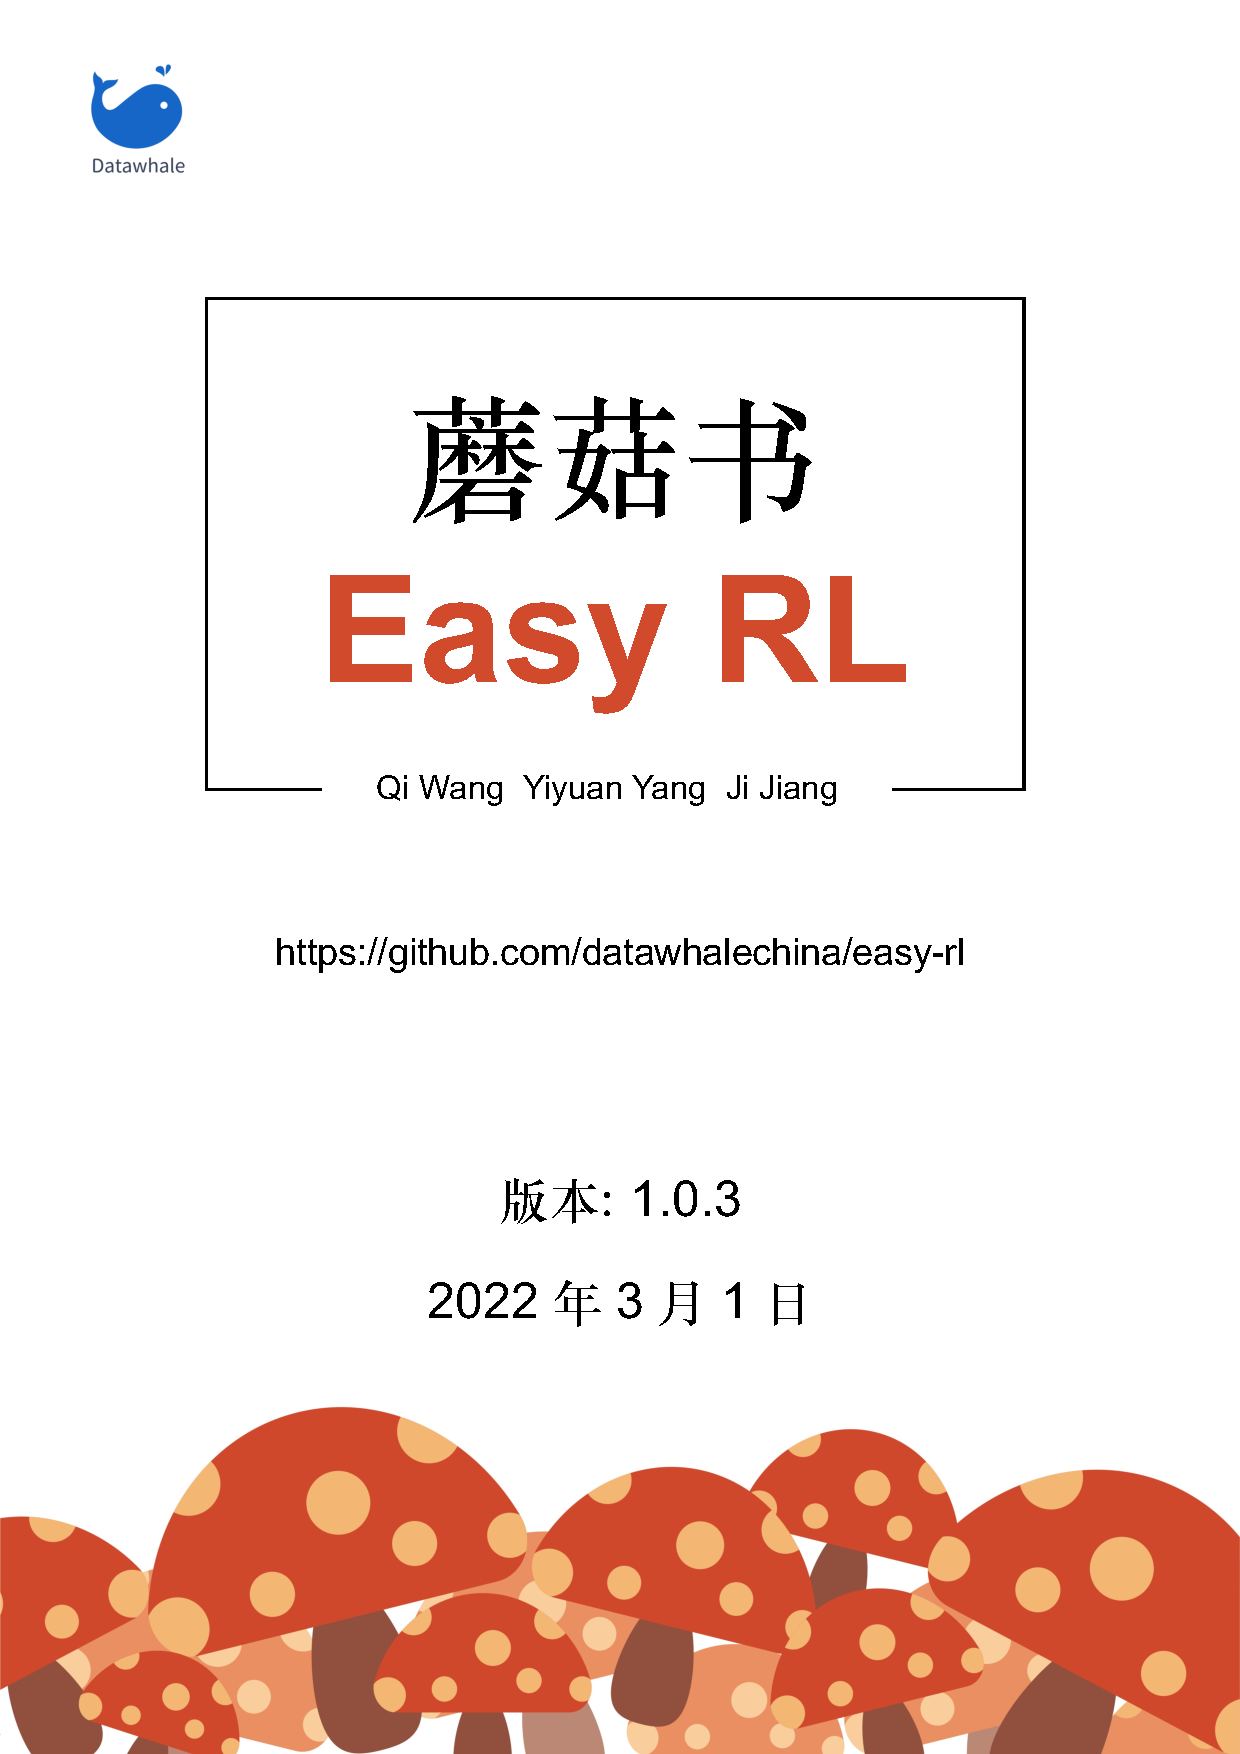
\includepdf[fitpaper=true]{res/cover.pdf}
    % \usepackage[a4paper, left=3.17cm, right=3.17cm, top=2.54cm, bottom=2.54cm]{geometry}
% \usepackage[T1]{fontenc}
% \usepackage{mathptmx}
% \usepackage{amsmath}
% \usepackage{amsfonts}
% \usepackage{chemformula}
% \usepackage{cite}
% \usepackage[colorlinks, linkcolor=black, anchorcolor=black, citecolor=black]{hyperref}
% \usepackage{graphicx}
% \setlength{\parskip}{0.5em}
% \title{Place Your Project Title at Here}
% \author{\textup{Sanlinc}}

\begin{titlepage}
	\newcommand{\HRule}{\rule{\linewidth}{0.5mm}}
	
\includegraphics[width=2cm]{res/logo_new.png}\\[1cm] 
	\center 
	\quad\\[1.5cm]
	% \textsl{\Large University of Chinese Academy of Sciences }\\[0.5cm] 
	
	\makeatletter
	\HRule \\[0.4cm]
	{ \huge \bfseries \@title}\\[0.4cm] 
	\HRule \\[1.5cm]
    % \Large \url{https://github.com/datawhalechina/easy-rl}\\[0.5cm] 
	\begin{minipage}{0.4\textwidth}
		\begin{flushleft} \large
			% \emph{Author:}\\
			% \@author 
		\end{flushleft}
	\end{minipage}
	~
	\begin{minipage}{0.4\textwidth}
		\begin{flushright} \large
			% \emph{Supervisor:} \\
			% \textup{Prof Yang}
		\end{flushright}
	\end{minipage}\\[3cm]
	\makeatother
	% {\large An Assignment submitted for the UCAS:}\\[0.5cm]
    \vfill  % 为了制造Whitespace 
	% {\large Datawhale强化学习小组~编著}\\[0.5cm]
    % {\Large Qi Wang~~~David Young~~~John Jim~编著}\\[0.5cm]
    % {\Large \href{https://github.com/qiwang067}{Qi Wang}~~~\href{https://github.com/yyysjz1997}{Yiyuan Yang}~~~\href{https://github.com/JohnJim0816}{Ji Jiang} ~编著}\\[0.5cm]
	{\Large 王琦~~~杨毅远~~~江季 ~编著}\\[0.5cm]
    {\Large  版本:1.0.2}\\[0.5cm]
	{\Large \today}\\[2cm] 
	
\end{titlepage}


    \thispagestyle{empty}
    \clearpage
    
    \section*{内容提要}
    强化学习作为机器学习及人工智能领域的一种重要方法,在游戏、自动驾驶、机器人路线规划等领域得到了广泛的应用。
    本书结合了李宏毅老师的《深度强化学习》、周博磊老师的《强化学习纲要》、李科浇老师的《百度强化学习》公开课的精华内容,在理论严谨的基础上深入浅出地介绍马尔可夫决策过程、蒙特卡洛方法、时序差分方法、Sarsa、Q学习等传统强化学习算法,以及策略梯度、近端策略优化、深度Q网络、深度确定性策略梯度等常见深度强化学习算法的基本概念和方法,并以大量生动有趣的例子帮助读者理解强化学习问题的建模过程以及核心算法的细节。此外,本书还提供较为全面的习题解答以及Python代码实现,可以让读者进行端到端、从理论到完全实践的全生态学习,充分掌握强化学习算法的原理并能进行实战。

    本书适合对强化学习感兴趣的读者阅读,也可以作为相关课程的配套教材。


    \clearpage
    \section*{前言}
    \renewcommand{\abstractname}{}
    % \begin{abstract}


    这是一本面向中文读者的强化学习教科书,为了使尽可能多的读者通过本书对强化学习有所了解,笔者试图尽可能少地使用数学知识,所涉及的公式都有详细的推导过程。本书适合相关专业的本科生和研究生,以及具有类似背景的对强化学习感兴趣的人士。

    全书共13章,大体上可分为2个部分:第1部分包括第1 \~{} 3章,介绍强化学习基础知识以及传统强化学习算法;第2部分包括第4 \~{} 13章,介绍深度强化学习算法以及常见问题的解决方法。第2部分各章相对独立,读者可根据自己的兴趣和时间情况选择阅读。
        
    书中大部分章配有习题和面试题,其可以帮助读者巩固知识。读者遇到某个不熟悉的概念时,还可以通过“关键词”部分来快速定位并掌握该概念。
        
    笔者以为,强化学习是一个理论与实践相结合的学科,读者不仅要理解其算法背后的一些数学原理,还要通过上机实践来实现算法。本书配有对应的 Python 代码实现,可以让读者通过动手实现各种经典的强化学习算法,充分掌握强化学习算法的原理。
        
    书中主要内容源于李宏毅老师的《深度强化学习》、周博磊老师的《强化学习纲要》以及李科浇老师的《百度强化学习》公开课。3位老师的强化学习公开课深入浅出、生动有趣,是强化学习的经典学习材料。感谢李宏毅、周博磊、李科浇3位老师的授权,使本书得以出版,能够造福更多对强化学习感兴趣的读者。
        
    本书由开源组织 Datawhale 的成员采用开源协作的方式完成,共历时一年有余,参与者包括3位编著者(笔者、杨毅远和江季)和两位 Datawhale 的小伙伴(谢文睿和马燕鹏)。在本书写作和出版过程中,人民邮电出版社的责任编辑郭媛给予了很多帮助,在此特向她致谢。
        
    强化学习发展迅速,笔者水平有限,书中难免有疏漏和表述不当的地方,还望各位读者批评指正。

\rightline{王琦~~~~~~~~~~~~~~~~~~}
\rightline{\today~~~~~~~~~~}

        % \subsection*{使用说明}
        % \begin{itemize}
        %     \item 
        %     第 4 章到第 11 章为\href{http://speech.ee.ntu.edu.tw/~tlkagk/courses_MLDS18.html}{李宏毅《深度强化学习》}的部分;
        %     \item 
        %     第 1 章和第 2 章根据\href{https://github.com/zhoubolei/introRL}{《强化学习纲要》}整理而来;
        %     \item 
        %     第 3 章和第 12 章根据\href{https://aistudio.baidu.com/aistudio/education/group/info/1335}{《百度强化学习》}整理而来。
        % \end{itemize}
        % \textbf{在线阅读地址:}\url{https://datawhalechina.github.io/easy-rl/}(内容实时更新)\\
        % \textbf{最新版PDF获取地址:}\url{https://github.com/datawhalechina/easy-rl/releases}
        % \subsection*{编委会}
        % \noindent
        % % \textbf{编委:}\href{https://github.com/qiwang067}{Qi Wang}、\href{https://github.com/yyysjz1997}{Yiyuan Yang}、\href{https://github.com/JohnJim0816}{Ji Jiang} 
        % \textbf{编委:}王琦、杨毅远、江季
        % % \textbf{编委:}jbb0523、juxiao、Majingmin、MrBigFan、shanry、Ye980226
        % \subsection*{致谢}
        % 特别感谢 \href{https://github.com/Sm1les}{Sm1les}、\href{https://github.com/LSGOMYP}{LSGOMYP} 对本项目的帮助与支持。
        % \noindent
        % \begin{center}
        % \vspace{1em}
        % 扫描下方二维码,然后回复关键词“\textbf{强化学习}”,即可加入“Easy-RL读者交流群”\\
        % \begin{figure}[hb]
        % \centering
        % 
\includegraphics[scale=0.2]{res/qrcode.jpeg}
        % \end{figure}
        % Datawhale\\一个专注于AI领域的开源组织\\
        % \vspace{2em}
        % \textbf{版权声明}\\本作品采用\href{http://creativecommons.org/licenses/by-nc-sa/4.0/}{\textbf{知识共享署名-非商业性使用-相同方式共享 4.0 国际许可协议}}进行许可。
        % \end{center}
    % \end{abstract}
    \thispagestyle{empty}
    \clearpage
    \setlength{\nomitemsep}{0.8cm}

\nomenclature[01]{$a$}{标量}
\nomenclature[02]{$\boldsymbol{a}$}{向量}
\nomenclature[03]{$\boldsymbol{A}$}{矩阵}
\nomenclature[04]{$\mathbb{R}$}{实数集}
\nomenclature[05]{$\underset{a}{\arg \max } f(a)$}{$f(a)$取最大值时 $a$ 的值}
\nomenclature[06]{$s$}{状态}
\nomenclature[07]{$a$}{动作}
\nomenclature[08]{$r$}{奖励}
\nomenclature[09]{$\pi$}{策略}
\nomenclature[10]{$\pi(s)$}{根据确定性策略 $\pi$ 在状态 $s$ 选取的动作}
\nomenclature[11]{$\pi(a|s)$}{根据随机性策略 $\pi$ 在状态 $s$ 选取的动作 $a$ 的概率}
\nomenclature[12]{$\gamma$}{折扣因子}
\nomenclature[13]{$\tau$}{轨迹}
\nomenclature[14]{$V_{\pi}(s)$}{状态 $s$ 在策略 $\pi$ 下的价值}
\nomenclature[15]{$Q_{\pi}(s,a)$}{状态 $s$ 在策略 $\pi$ 下采取动作 $a$ 的价值}
\nomenclature[16]{$G_{t}$}{时刻 $t$ 时的回报}
\nomenclature[17]{$\pi_{\theta}$}{参数$\theta$ 对应的策略}
\nomenclature[18]{$J({\theta})$}{策略$\pi_{\theta}$的性能度量}

\printnomenclature[4in]





    \tableofcontents % 生成目录
    % \thispagestyle{empty}
    \clearpage

    % \section{绪论}
\setcounter{page}{1}
\subsection{强化学习概述}

\kw{强化学习(reinforcement learning,RL)} 是广义机器学习的一个领域,注意这里广义机器学习泛指涵盖几乎所有人工智能方法的领域,包括狭义的机器学习(例如线性模型,支持向量机等)和深度学习等等。强化学习涉及智能体如何在环境中采取动作以便最大化累积奖励的概念。智能体在学习的过程中不会被预先告知应该采取何种动作,而是通过\kw{试错(trial-and-error)}去发现采取哪种动作会使得对应的奖励最大。举一个典型的例子,就好比学生在学校学一门课,经验事实告诉我们最终的目标是在期末考试拿到尽可能高的分数。学生在这个过程中充当智能体,采取的动作或策略可以是中规中矩的上课听讲并按时完成作业,也可以再花点力气预习内容并上课认真听讲按时完成作业,还可以是不上课每天尽情玩乐,而最终期末考试分数就是一个奖励,决定最终奖励高低的则取决于采取动作或者学习策略的最优程度,当然实际的问题往往要复杂得多。此外智能体采取的动作也往往会影响到环境的状态和\kw{即时奖励(immediate reward)},比如我们学习了一天的功课之后脑袋会感到充实会有成就感,而我们尽情玩乐了一天之后会获得短暂的快乐并伴随着一定的空虚感,或者说上课认真听讲的同学会发现老师的态度会比较友好,不遵守课堂纪律的同学会受到老师的批评等等都说明采取的动作会影响到环境的状态。而即时奖励则与\kw{长期奖励(long-term)}相对,其中期末考试的分数可以看做长期奖励,比如我们学习了一天会潜在地影响到最终的期末分数但是不能看到立竿见影的效果。我们能迅速看到的效果是学习了一章的内容然后去做对应章节的作业,作业的评分就相当于即时奖励,再比如我们玩了一天的游戏也能享受肾上腺素和多巴胺带来的生理性快乐,这也可以看作即时奖励。并且即便是玩了一天的游戏对于期末分数也就是长期奖励的影响也是微乎其微的,也许某位同学在学期第一天玩了一天的游戏之后痛定思痛并在接下来的每一天刻苦学习,那么他很大概率也是能获得比较高的最终奖励的。这就是强化学习除了试错之外的一个重要特性,即\kw{延时奖励(delayed reward)}。注意试错是相对于最终目标而言的,比如我们知道如果平时作业得高分就说明这段时间学习效果好,一直作业得高分下去期末分数必然也会很高,因此相对于期末分数这个最终目标来说平时作业的高分是一种即时奖励。如果我们玩了一天的游戏,虽然我们收获了快乐,获得了生理性的即时奖励,但这种生理性的即时奖励相对于最终目标往往是起到反作用的,而这种情况下我们的平时作业分会比较差,相当于得到了一个比较低甚至是负数的奖励(也就是惩罚)。我们通过这些即时奖励或惩罚来判断我们每一步的动作或策略是否错误,然后一步一步地直至达到最终的目标,这就是试错的涵义。

强化学习是一个强交互过程,擅长解决序列决策问题。严格来讲,强化学习隶属于动态系统理论的范畴,涉及马尔可夫决策问题(序列决策问题的数学描述)的最优化控制,这点在后面马尔可夫过程相关章节中会详细展开。在这个最优化控制过程中,智能体必须能够感知到环境的状态并采取合适的动作,对应的动作又会影响到环境的状态,而能够解决这一类问题的方法我们都统称为强化学习方法。

\subsection{强化学习与监督学习}

强化学习是三种基本机器学习范式之一,另外两种是监督学习与无监督学习。如\figref{fig:supervise_learning}所示,监督学习是从一堆打好标签或者标注的训练数据中来学习的,这些标签通常由经验丰富的专家来确定,表示在某种环境状态下智能体应当采取的动作,更确切地说,是表示某种环境状态对应的分类,然后推断一些在训练集中没有出现的状态。但是在交互问题中打标签是不切实际的,在一些未知的状态下,智能体必须学会从自身的经验中学习,这就是强化学习的独特之处。就好比我们吃西瓜,假设在我们对西瓜没有任何先验认知的情况下,即前面所说的未知的状态或领域,我们是不知道哪种西瓜更好吃的。这种情况下,我们只能通过尝试来确定哪种西瓜好吃,好比神农尝百草一样,我们是尝百瓜之后才能练就一身仅通过西瓜外观就能判断西瓜好不好吃的本领,这个本领的学习过程是需要强化学习的。在我们成为吃瓜老手也就是经验丰富的专家之后,我们会总结一些经验,比如瓜皮颜色较深的、瓜瓤很红的、瓜敲起来声音较清脆往往会比较好吃,把瓜皮、瓜瓤颜色、敲瓜声音作为输入特征,把好吃与不好吃作为输出分类,这就是监督学习所做的事情。

\begin{figure}[hbt]
    \centering
    \includegraphics[width=0.5\linewidth]{ch1/figs/supervise_learning.png}
    \caption{监督学习示例}
    \label{fig:supervise_learning}
\end{figure}

\subsection{强化学习与无监督学习}

无监督学习旨在发现数据样本的一些潜在特征然后将这些样本自动聚类,例如一个无监督学习在“吃瓜”的过程中也许发现了通过瓜皮、瓜瓤颜色、敲瓜声音这些特征能够将西瓜分成不同的几类,然后将它们划分开来。乍一看,无监督学习似乎跟强化学习很类似,因此有时候强化学习也被误解为一种无监督学习模型。但强化学习本质上其最终目标是最大化智能体在交互过程中获得的累积奖励而不是挖掘样本的潜在特征,尽管在智能体获得的经验中挖掘潜在特征会有所帮助,但是无监督学习同监督学习一样,本身并不具备处理交互问题的能力。


\subsection{强化学习的例子}

我们再举一些例子来帮助读者加深对强化学习的理解,并且读者们仔细想想也会发现生活中处处是强化学习。比如一个围棋下棋时,每次落子前都会在脑中演练接下来十几步可能出现的棋局,然后做出最佳的落子选择,然后当对手落完子之后会自我反馈对手的落子是否在计算之内,如果在计算之内那么又重复演练进行下一个落子,如果不在就可能学习到了新的经验以便提高自己的棋力。顺便提一句,其中演练的过程我们在强化学习中通常称之为规划(planning),不在计算之内然后学习新经验的情况称之为学习(learning),具体细节我们会在后面的章节中展开说明。再比如一个高级扫地机器人有时会决策是否到下一个房间继续打扫垃圾,还是返回到充电口处自行充电。这种决策主要基于它对自身现有电量的判断以及根据已有的经验(之前走过的房间和观测到充电口的位置等等)来分析如何以最快最方便的路径返回到充电口处充电,这就是强化学习会把探索过的状态等形成经验从而便于未来做出最优的决策。再比如我们开车从杭州到上海,通常会打开电子地图导航,到了一段高速导航会提示应当走哪条道保持多少速度,到了一个路口会提示左转右转,遇到一些新修的路面时,电子地图往往未来得及同步数据会给出错误的提示,此时就需要结合我们自身的经验来判断如何行驶了。这个例子说明我们在与环境互动的过程中会持续收到反馈,当出现一些未知的情形时,我们可以同样可以利用学习到的经验来决策,甚至是结合一些非机器学习的经验判断,比如我们知道红灯停绿灯行,此时我们可以不需要强化学习模型学出来这个策略,直接根据规则或其他的模型判断决策即可,这就是强化学习的灵活之处,并且常常在一些复杂的强化学习智能竞赛中运用到这项技巧(trick)。


\subsection{强化学习的历史}

在Sutton教授等人的书\upcite{rl_mit}中讨论了强化学习历史形成的三条线:1)通过试错学习;2)最优化控制问题;3)时序差分(Temporal Difference)方法。这三条时间线最后在1980年代汇聚一堂,开始形成我们今天所讨论的强化学习概念雏形。由于 Sutton 教授在他的书中已经讲述得比较清楚,加之这也不是本书的重点内容,因此这里会简要罗列一下这三条时间线中的一些重要节点,感兴趣的读者可以在茶余饭后查阅相关资料对强化学习历史进行深入的考究。

\subsubsection{试错学习}

前面讲到,试错学习作为强化学习的重要特征之一,是具有一段独立的历史故事的。试错学习最初由\upcite{Thorndike:1911}等人(1911)受到生物学启发定义,举个简单的例子,把蚯蚓放在包含一条分岔口的盒子里,蚯蚓只能向左或向右爬行,在左边放上食物,在右边放上释放弱电的设备,当蚯蚓往左爬的时候获取食物即奖励,往右爬的时候会被电击受到惩罚,每次受到奖励或惩罚之后把蚯蚓重新放回起始点并继续向左或向右爬行。一开始蚯蚓可能没有意识到左边会拿到奖励右边会受到惩罚这一点,每次都会随机往两边爬行,直到累积足够的次数或经验之后蚯蚓就学会了每次只往左边爬行了,这个过程就是试错的过程,在我们的生活中屡见不鲜。试错概念后面在1961年被 Minsky 等人\upcite{Minsky:1961:ire}引入到机器学习模拟(Machine Learning analogue)中并用于处理信用分配问题(Credit Assignment Problem),其中信用分配问题也是目前强化学习研究的问题分支之一。与此同时,试错的计算过程也被泛化到了模式识别问题中(https://dl.acm.org/doi/abs/10.1145/1455292.1455309),主要利用试错信息来帮助监督学习更新相关参数。

TODO https://towardsdatascience.com/reinforcement-learning-fda8ff535bb6#5554

\subsubsection{强化学习的应用}
讲一些现代应用,游戏、推荐系统、派单、组合优化、自动驾驶等等
\subsection{强化学习要素}
\subsubsection{智能体与环境}
\subsubsection{策略}
\subsubsection{奖励}
\subsection{学习与规划}
\subsection{探索与利用}
\subsection{实战:学会用 VS Code 开发强化学习算法}
\subsubsection{ VS Code 安装}
\subsubsection{ VS Code 搭建Python环境}
\subsection{关键词}
\subsection{习题}
\subsection{面试题}
\subsection{本章小结}
    % \include{ch2}
    % \section{表格型方法}
\subsection{蒙特卡洛方法}
\subsection{时序差分方法}
\subsection{ Q-learning 算法}
\subsection{ Sarsa 算法}
\subsection{ Dyna-Q 算法}
\subsubsection{有模型与免模型}
\subsection{实战:Q-learning 算法}
\subsection{实战:Sarsa 算法}
\subsection{实战:Dyna-Q 算法}
\subsection{关键词}
\subsection{习题}
\subsection{面试题}
\subsection{本章小结}
    % \include{ch4}
    % \section{ DQN 算法进阶}
\subsection{ Double DQN 算法}

\subsection{ Dueling DQN 算法}

\subsection{ PER DQN 算法}
\subsection{ HER DQN 算法}

\subsection{ Noisy DQN 算法}
\subsection{ QR DQN 算法}
\subsection{ Rainbow DQN 算法}


\subsection{实战:Double DQN 算法}

\subsection{实战:Dueling DQN 算法}

\subsection{实战:PER DQN 算法}

\subsection{实战:HER DQN 算法}
\subsection{实战:Noisy DQN 算法}
\subsection{实战:QR DQN 算法}
\subsection{实战:Rainbow DQN 算法}

\subsection{关键词}
\subsection{习题}
\subsection{面试题}
\subsection{本章小结}
    \section{马尔可夫决策过程}

\figref{fig:rl_pic} 介绍了强化学习中智能体与环境之间的交互过程,智能体观测到环境的状态后,它会采取动作,然后环境根据智能体采取的动作进入到下一个状态,并反馈出对应的奖励信号。举一个踢足球的例子,假设我们一开始什么也不会,但想要学习罚点球,也就是在点球点处将球踢进球门里去,每次练习开始我们观测到球和球门的位置,并尝试调整角度将球踢出去。踢出去之后球的位置会发生变化,根据球和球门的位置我们可以接收到反馈,比如球是进球门了还是踢飞了。接着我们将球重新放回点球点处继续练习,并根据上一次收到的反馈调整我们的射门动作,如此循环交互,直到学会将球踢进球门为止。在这个过程中,我们人就相当于是智能体,球和球门的位置就是人观测到的状态,将球踢出去就是一个动作,而球、球门和球场组成整个环境,每次采取动作后接收到的反馈可以数值化成一个奖励信号,进球门了就是正的奖励,踢飞了或者没踢进就是负的奖励,也就是惩罚。生活中的很多问题都可以用这样一段持续的交互过程来描述,而这个交互过程在数学上可以用马尔可夫决策过程(Markov decision process,MDP),而用于解决 MDP 问题的方法都可以被认为是强化学习方法,因此\kw{ MDP 是强化学习的基本问题模型之一}。换句话说,要想用强化学习算法解决某个实际问题,我们必须首先将这个问题描述或者建模成一个马尔可夫决策过程。顺便说一句,之所以说MDP 是强化学习的基本问题模型之一,这里之一的意思是在更多复杂的情况中比如多智能体环境我们需要把问题建模成一个 MDP 的衍生版本,比如 部分可观测马尔可夫决策过程(partially observable Markov decision processes,POMDP) 以及马尔可夫博弈等等,但广义上来说都属于马尔可夫决策过程,具体在后面讲述相关内容时再详细展开。


\begin{figure}[hbt]
  \centering
  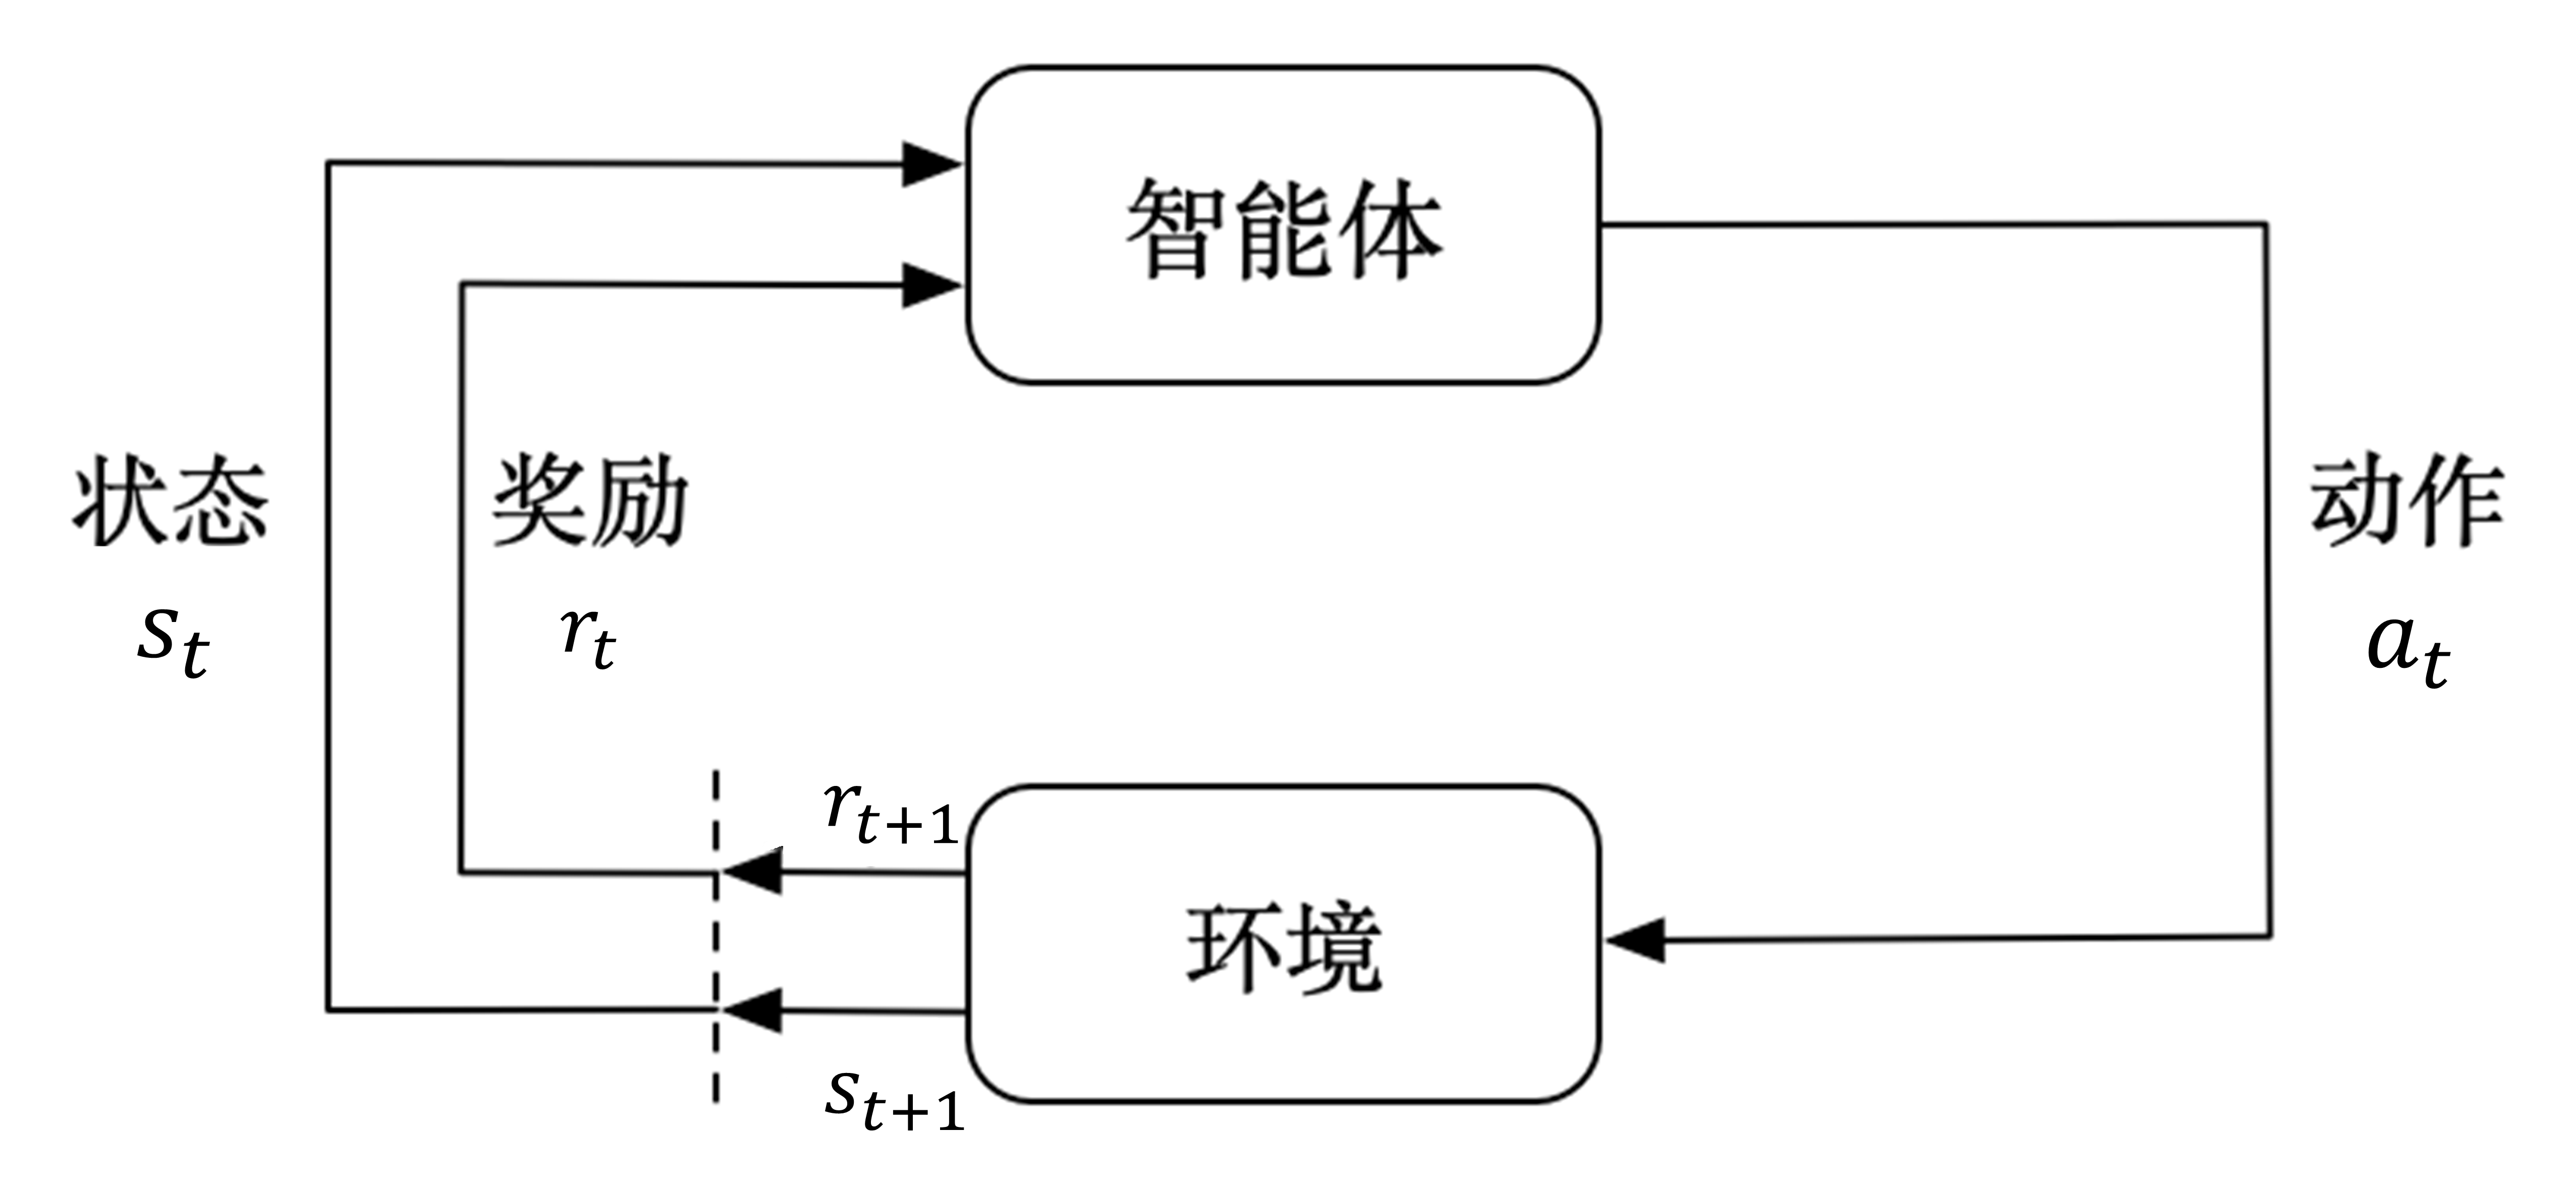
\includegraphics[width=0.5\linewidth]{ch2/figs/rl_pic.png}
  \caption{智能体与环境之间的交互}
  \label{fig:rl_pic}
\end{figure}


本章将介绍马尔可夫决策过程(Markov decision process,MDP)。在介绍马尔可夫决策过程之前,我们先介绍它的简化版本:马尔可夫过程(Markov process,MP)以及马尔可夫奖励过程(Markov reward process,MRP)。通过这两种过程的铺垫,我们可以更容易理解马尔可夫决策过程。
\subsection{马尔可夫过程}
\subsubsection{马尔可夫性质}
\kw{马尔可夫性质(Markov property)}是概率论中的一个概念,指的是当一个随机过程在给定当前状态及所有过去状态情况下,其未来状态的条件概率分布仅依赖于当前状态。换句话说,在给定当前状态下,它与过去状态(即该过程的历史路径)是条件独立的。

以离散随机过程为例,假设随机变量 $X_0,X_1,\cdots,X_T$构成一个随机过程。这些随机变量的所有可能取值的集合被称为状态空间(state space)。如果 $X_{t+1}$ 对于过去状态的条件概率分布仅是 $X_t$ 的一个函数,则
\begin{equation}
  \label{eq:}
  p\left(X_{t+1}=x_{t+1} \mid X_{0:t}=x_{0: t}\right)=p\left(X_{t+1}=x_{t+1} \mid X_{t}=x_{t}\right)
\end{equation}
其中,$X_{0:t}$ 表示变量集合 $X_{0}, X_{1}, \cdots, X_{t}$,$x_{0: t}$ 为在状态空间中的状态序列 $x_{0}, x_{1}, \cdots, x_{t}$。

马尔可夫性质是所有马尔可夫过程的基础。这种性质看似深奥,其实在我们日常生活中也司空见惯,比如一天内,我晚餐的食量由午餐的时间和摄入直接决定,而不由早餐的时间和摄入间接决定(因为早餐摄入的食物在晚餐前就已经消化掉了),这样一来一日三餐的摄入就可以简单看作一个马尔可夫过程。

\subsubsection{马尔可夫链}
% 如果一个状态转移是符合马尔可夫的,也就是满足条件:
马尔可夫过程是一组具有马尔可夫性质的随机变量序列 $s_1,\cdots,s_t$,其中下一个时刻的状态$s_{t+1}$只取决于当前状态 $s_t$。我们设状态的历史为 $h_{t}=\left\{s_{1}, s_{2}, s_{3}, \ldots, s_{t}\right\}$($h_t$ 包含了之前的所有状态),则马尔可夫过程满足条件:
\begin{equation}
  \label{eq:}
  p\left(s_{t+1} \mid s_{t}\right) =p\left(s_{t+1} \mid h_{t}\right)
\end{equation}
从当前 $s_t$ 转移到 $s_{t+1}$,它是直接就等于它之前所有的状态转移到 $s_{t+1}$。

离散时间的马尔可夫过程也称为\kw{马尔可夫链(Markov chain)}。马尔可夫链是最简单的马尔可夫过程,其状态是有限的。例如,\figref{fig:mp_example} 里面有4个状态,这4个状态在 $s_1,s_2,s_3,s_4$ 之间互相转移。比如从 $s_1$ 开始,$s_1$ 有 0.1 的概率继续存留在 $s_1$ 状态,有 0.2 的概率转移到 $s_2$,有 0.7 的概率转移到 $s_4$ 。如果 $s_4$ 是我们的当前状态,它有 0.3 的概率转移到 $s_2$,有 0.2 的概率转移到 $s_3$,有 0.5 的概率留在当前状态。

\begin{figure}[htb]
  \centering
  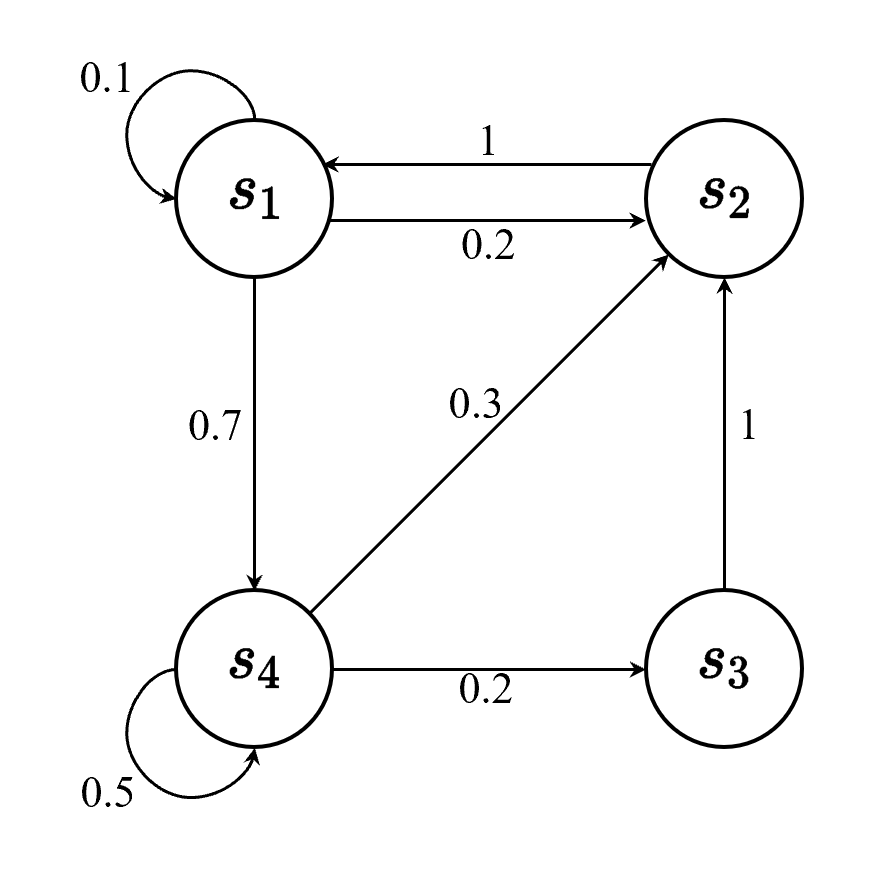
\includegraphics[width=0.3\linewidth]{ch2/figs/m_chain_example.png}
  \caption{马尔可夫链示例}
  \label{fig:mp_example}
\end{figure}

我们可以用\kw{状态转移矩阵(state transition matrix)}$\boldsymbol{P}$ 来描述状态转移 $p\left(s_{t+1}=s^{\prime} \mid s_{t}=s\right)$:
\begin{equation}
  \boldsymbol{P}=\left(\begin{array}{cccc}
    p\left(s_{1} \mid s_{1}\right) & p\left(s_{2} \mid s_{1}\right) & \ldots & p\left(s_{N} \mid s_{1}\right) \\
    p\left(s_{1} \mid s_{2}\right) & p\left(s_{2} \mid s_{2}\right) & \ldots & p\left(s_{N} \mid s_{2}\right) \\
    \vdots & \vdots & \ddots & \vdots \\
    p\left(s_{1} \mid s_{N}\right) & p\left(s_{2} \mid s_{N}\right) & \ldots & p\left(s_{N} \mid s_{N}\right)
    \end{array}\right)
  \label{eq:1}
\end{equation}
状态转移矩阵类似于条件概率(conditional probability),它表示当我们知道当前我们在状态 $s_t$ 时,到达下面所有状态的概率。所以它的每一行描述的是从一个节点到达所有其他节点的概率。

\subsection{马尔可夫奖励过程} 

\kw{马尔可夫奖励过程(Markov reward process, MRP)}是马尔可夫链加上奖励函数。在马尔可夫奖励过程中,状态转移矩阵和状态都与马尔可夫链一样,只是多了\kw{奖励函数(reward function)}。奖励函数 $R$ 是一个期望,表示当我们到达某一个状态的时候,可以获得多大的奖励。这里另外定义了折扣因子 $\gamma$ 。如果状态数是有限的,那么 $R$ 可以是一个向量。

\subsubsection{回报与价值函数}

这里我们进一步定义一些概念。\kw{范围(horizon)} 是指一个回合的长度(每个回合最大的时间步数),它是由有限个步数决定的。
\kw{回报(return)}可以定义为奖励的逐步叠加,假设时刻$t$后的奖励序列为$r_{t+1},r_{t+2},r_{t+3},\cdots$,则回报为
\begin{equation}
  G_{t}=r_{t+1}+\gamma r_{t+2}+\gamma^{2} r_{t+3}+\gamma^{3} r_{t+4}+\ldots+\gamma^{T-t-1} r_{T}
  \label{eq:}
\end{equation}
其中,$T$是最终时刻,$\gamma$ 是折扣因子,越往后得到的奖励,折扣越多。这说明我们更希望得到现有的奖励,对未来的奖励要打折扣。
当我们有了回报之后,就可以定义状态的价值了,就是\kw{状态价值函数(state-value function)}。对于马尔可夫奖励过程,状态价值函数被定义成回报的期望,即
\begin{equation}
  \begin{aligned}
    V^{t}(s) &=\mathbb{E}\left[G_{t} \mid s_{t}=s\right] \\
    &=\mathbb{E}\left[r_{t+1}+\gamma r_{t+2}+\gamma^{2} r_{t+3}+\ldots+\gamma^{T-t-1} r_{T} \mid s_{t}=s\right]
    \end{aligned}
  \label{eq:}
\end{equation}
其中,$G_t$ 是之前定义的\kw{折扣回报(discounted return)}。我们对$G_t$取了一个期望,期望就是从这个状态开始,我们可能获得多大的价值。所以期望也可以看成未来可能获得奖励的当前价值的表现,就是当我们进入某一个状态后,我们现在有多大的价值。

我们使用折扣因子的原因如下。第一,有些马尔可夫过程是带环的,它并不会终结,我们想避免无穷的奖励。第二,我们并不能建立完美的模拟环境的模型,我们对未来的评估不一定是准确的,我们不一定完全信任模型,因为这种不确定性,所以我们对未来的评估增加一个折扣。我们想把这个不确定性表示出来,希望尽可能快地得到奖励,而不是在未来某一个点得到奖励。
第三,如果奖励是有实际价值的,我们可能更希望立刻就得到奖励,而不是后面再得到奖励(现在的钱比以后的钱更有价值)。
最后,我们也更想得到即时奖励。有些时候可以把折扣因子设为 0($\gamma=0$),我们就只关注当前的奖励。
我们也可以把折扣因子设为 1($\gamma=1$),对未来的奖励并没有打折扣,未来获得的奖励与当前获得的奖励是一样的。
折扣因子可以作为强化学习智能体的一个超参数(hyperparameter)来进行调整,通过调整折扣因子,我们可以得到不同动作的智能体。

在马尔可夫奖励过程里面,我们如何计算价值呢?如\figref{fig:fig2.11} 所示,马尔可夫奖励过程依旧是状态转移,其奖励函数可以定义为:智能体进入第一个状态 $s_1$ 的时候会得到 5 的奖励,进入第七个状态 $s_7$ 的时候会得到 10 的奖励,进入其他状态都没有奖励。我们可以用向量来表示奖励函数,即

\begin{equation}
  \label{eq:}
  \boldsymbol{R}=[5,0,0,0,0,0,10]
\end{equation}

\begin{figure}[hbt]
  \centering
  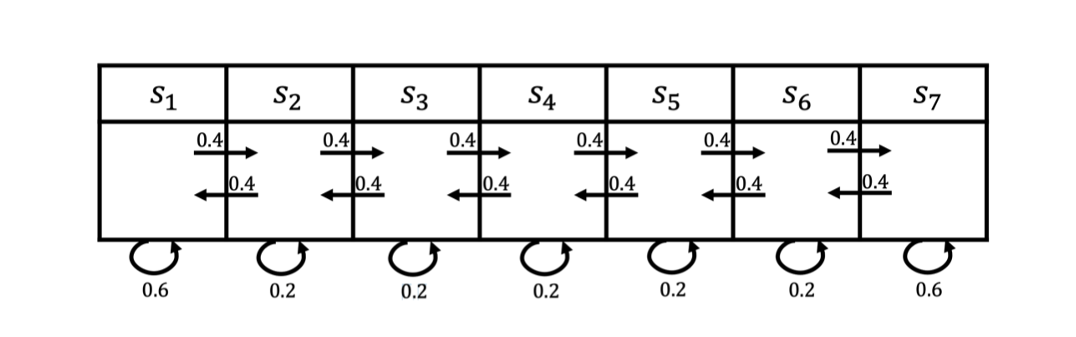
\includegraphics[width=0.7\linewidth]{ch2/figs/2.11.png}
  \caption{马尔可夫奖励过程的例子}
  \label{fig:fig2.11}
\end{figure}

我们对 4 步的回合($\gamma=0.5$)来采样回报 $G$。
% \begin{enumerate}[label=\protect\circled{\arabic*}]

  (1)$s_{4}, s_{5}, s_{6}, s_{7} \text{的回报}: 0+0.5\times 0+0.25 \times 0+ 0.125\times 10=1.25$

  (2)$s_{4}, s_{3}, s_{2}, s_{1} \text{的回报}: 0+0.5 \times 0+0.25\times 0+0.125 \times 5=0.625$

  (3)$s_{4}, s_{5}, s_{6}, s_{6} \text{的回报}: 0+0.5\times 0 +0.25 \times 0+0.125 \times 0=0$
% \end{enumerate}

我们现在可以计算每一个轨迹得到的奖励,比如我们对轨迹 $s_4,s_5,s_6,s_7$ 的奖励进行计算,这里折扣因子是 0.5。
在 $s_4$ 的时候,奖励为0。
下一个状态 $s_5$ 的时候,因为我们已经到了下一步,所以要把 $s_5$ 进行折扣,$s_5$ 的奖励也是0。
然后是 $s_6$,奖励也是0,折扣因子应该是0.25。
到达 $s_7$ 后,我们获得了一个奖励,但是因为状态 $s_7$ 的奖励是未来才获得的奖励,所以我们要对之进行3次折扣。
最终这个轨迹的回报就是 1.25。类似地,我们可以得到其他轨迹的回报。

这里就引出了一个问题,当我们有了一些轨迹的实际回报时,怎么计算它的价值函数呢?比如我们想知道 $s_4$ 的价值,即当我们进入 $s_4$ 后,它的价值到底如何?一个可行的做法就是我们可以生成很多轨迹,然后把轨迹都叠加起来。比如我们可以从 $s_4$ 开始,采样生成很多轨迹,把这些轨迹的回报都计算出来,然后将其取平均值作为我们进入 $s_4$ 的价值。这其实是一种计算价值函数的办法,也就是通过蒙特卡洛(Monte Carlo,MC)采样的方法计算 $s_4$ 的价值。

\subsubsection{马尔可夫奖励过程的例子} 

如\figref{fig:mrp_example} 所示,如果我们在马尔可夫链上加上奖励,那么到达每个状态,我们都会获得一个奖励。我们可以设置对应的奖励,比如智能体到达状态 $s_1$时,可以获得 5 的奖励;到达 $s_7$ 的时候,可以得到 10 的奖励;到达其他状态没有任何奖励。
因为这里的状态是有限的,所以我们可以用向量 $\boldsymbol{R}=[5,0,0,0,0,0,10]$ 来表示奖励函数,$\boldsymbol{R}$表示每个状态的奖励大小。

我们通过一个形象的例子来理解马尔可夫奖励过程。我们把一艘纸船放到河流之中,它就会随着水流而流动,它自身是没有动力的。所以我们可以把马尔可夫奖励过程看成一个随波逐流的例子,当我们从某一个点开始的时候,纸船就会随着事先定义好的状态转移进行流动,它到达每个状态后,我们都有可能获得一些奖励。

\begin{figure}[hbt]
  \centering
  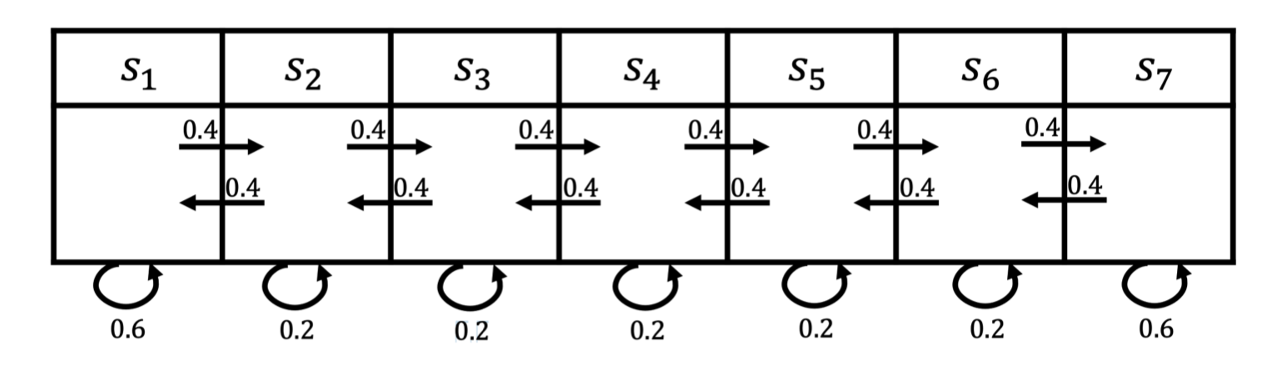
\includegraphics[width=0.5\linewidth]{ch2/figs/2.8}
  \caption{马尔可夫奖励过程的例子}
  \label{fig:mrp_example}
\end{figure}

\subsection{马尔可夫决策过程} 
相对于马尔可夫奖励过程,马尔可夫决策过程多了决策(决策是指动作),其他的定义与马尔可夫奖励过程的是类似的。此外,状态转移也多了一个条件,变成了$p\left(s_{t+1}=s^{\prime} \mid s_{t}=s,a_{t}=a\right)$。未来的状态不仅依赖于当前的状态,也依赖于在当前状态智能体采取的动作。马尔可夫决策过程满足条件:
\begin{equation}
  \label{eq:}
  p\left(s_{t+1} \mid s_{t}, a_{t}\right) =p\left(s_{t+1} \mid h_{t}, a_{t}\right)   
\end{equation}

对于奖励函数,它也多了一个当前的动作,变成了 $R\left(s_{t}=s, a_{t}=a\right)=\mathbb{E}\left[r_{t} \mid s_{t}=s, a_{t}=a\right]$。当前的状态以及采取的动作会决定智能体在当前可能得到的奖励多少。


\subsubsection{马尔可夫决策过程中的策略} 

策略定义了在某一个状态应该采取什么样的动作。知道当前状态后,我们可以把当前状态代入策略函数来得到一个概率,即 
\begin{equation}
  \pi(a \mid s)=p\left(a_{t}=a \mid s_{t}=s\right)
  \label{eq:}
\end{equation}
概率代表在所有可能的动作里面怎样采取行动,比如可能有 0.7 的概率往左走,有 0.3 的概率往右走,这是一个概率的表示。
另外策略也可能是确定的,它有可能直接输出一个值,或者直接告诉我们当前应该采取什么样的动作,而不是一个动作的概率。
假设概率函数是平稳的(stationary),不同时间点,我们采取的动作其实都是在对策略函数进行采样。

已知马尔可夫决策过程和策略 $\pi$,我们可以把马尔可夫决策过程转换成马尔可夫奖励过程。
在马尔可夫决策过程里面,状态转移函数 $P(s'|s,a)$ 基于它当前的状态以及它当前的动作。因为我们现在已知策略函数,也就是已知在每一个状态下,可能采取的动作的概率,所以我们就可以直接把动作进行加和,去掉 $a$,这样我们就可以得到对于马尔可夫奖励过程的转移,这里就没有动作,即
\begin{equation}
  P_{\pi}\left(s^{\prime} \mid s\right)=\sum_{a \in A} \pi(a \mid s) p\left(s^{\prime} \mid s, a\right)
  \label{eq:}
\end{equation}

对于奖励函数,我们也可以把动作去掉,这样就会得到类似于马尔可夫奖励过程的奖励函数,即
\begin{equation}
  r_{\pi}(s)=\sum_{a \in A} \pi(a \mid s) R(s, a)
  \label{eq:}
\end{equation}

\subsubsection{马尔可夫决策过程和马尔可夫过程/马尔可夫奖励过程的区别} 
马尔可夫决策过程里面的状态转移与马尔可夫奖励过程以及马尔可夫过程的状态转移的差异如\figref{fig:fig2.21} 所示。
马尔可夫过程/马尔可夫奖励过程的状态转移是直接决定的。比如当前状态是 $s$,那么直接通过转移概率决定下一个状态是什么。
但对于马尔可夫决策过程,它的中间多了一层动作 $a$ ,即智能体在当前状态的时候,首先要决定采取某一种动作,这样我们会到达某一个黑色的节点。到达这个黑色的节点后,因为有一定的不确定性,所以当智能体当前状态以及智能体当前采取的动作决定过后,智能体进入未来的状态其实也是一个概率分布。在当前状态与未来状态转移过程中多了一层决策性,这是马尔可夫决策过程与之前的马尔可夫过程/马尔可夫奖励过程很不同的一点。在马尔可夫决策过程中,动作是由智能体决定的,智能体会采取动作来决定未来的状态转移。

\begin{figure}[hbt]
  \centering
  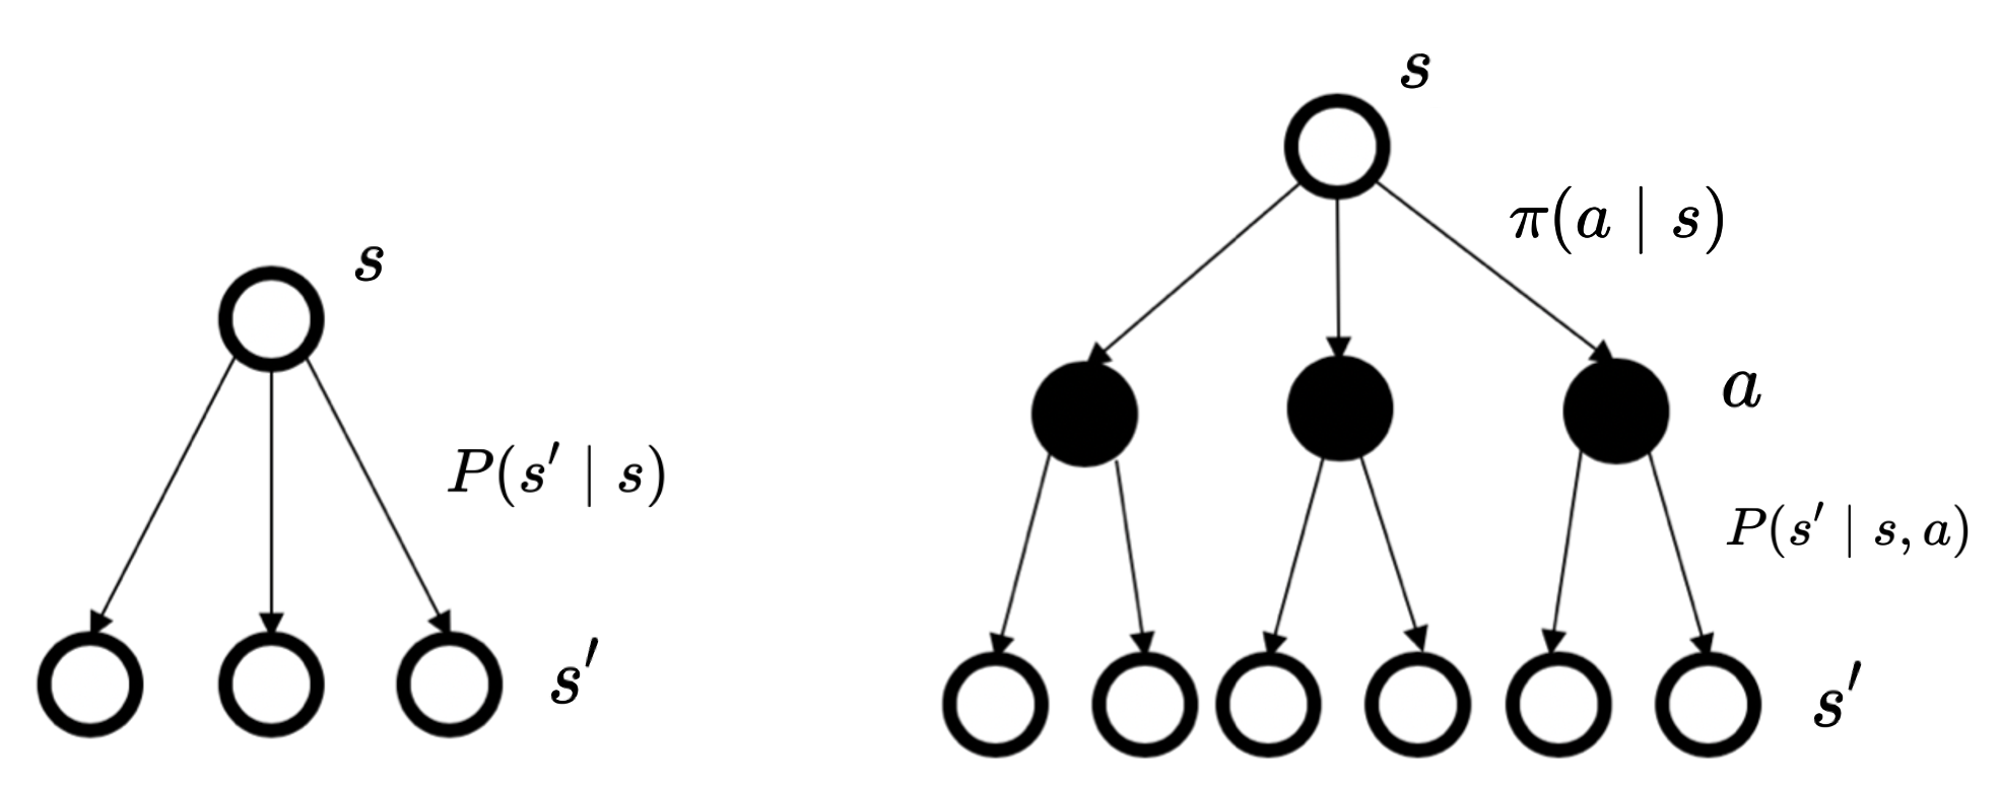
\includegraphics[width=0.6\linewidth]{ch2/figs/2.21.png}
  \caption{马尔可夫决策过程与马尔可夫过程/马尔可夫奖励过程的状态转移的对比}
  \label{fig:fig2.21}
\end{figure}

    % \section{ DQN 算法}

我们知道求解强化学习的一种思路就是优化状态价值函数 $V(s)$ 或动作价值函数 $Q(s,a)$,而传统强化学习算法是以表格的形式存储这些价值函数的,这导致最终优化的对象本身就具有一定的局限性。首先表格形式的价值函数是离散的,存储的状态之间比较独立,对于一些近似状态的拟合就难以体现出关联性。以学生上下课为例,对于学生这个智能体来讲,数学课和物理课这两种状态其实应该是近似的,因为对于考高分这个长期目标来说,数学课和物理课具有类似的价值(都涉及复杂的公式和逻辑),换句话说对应的状态-价值函数应当类似。但是如果用表格形式存储的话,在更新价值函数的过程中是体现不出来这些关联性的。其次表格能够存储的状态-动作对是有限的,这受限于计算机的内存空间,这样一来在实际的强化学习任务中往往涉及成千上万个状态-动作对,如果都用表格来存储的话,会增加很多的计算和内存成本。在这种情况下,最好的办法就是换一种价值函数的表示形式,而深度神经网络就能很好地解决这个问题。深度神经网络本质上就是一个复杂的非线性函数,比较契合价值函数本身的定义,此外使用深度神经网络也能顺便解析一些复杂的状态及其内在的关联性,例如解决图像输入的卷积神经网络等等,因此目前主流的强化学习算法都是以深度神经网络为基础的算法,我们称作深度强化学习算法(DRL,Deep Reinforcement Learning)。

\subsection{深度学习基础}

在本章中会详细讲解一种经典的 DRL 算法,即 DQN 算法,在介绍该算法之前我们先简单了解一些深度学习的基础。注意,这里只是简单做一个入门的铺垫,如果读者们后面想深入做强化学习算法研究或者相关应用时,还是有必要进一步了解更多的深度网络模型的,例如能够识别图像状态输入的卷积神经网络、解析时间序列状态输入的循环神经网络等等。
\subsubsection{线性模型}

首先介绍线性模型,线性模型是最简单的一类机器学习模型,可以将其视为单层的神经网络。在线性模型中最基础的两个模型就是线性回归和逻辑回归,通常分别用于解决回归和分类问题,尽管后者也可以用来解决回归问题。回归模型的输出是一个连续的值,而分类模型的输出是离散的值,用于表示分类。本质上来说回归模型和分类模型是一样的,分类模型可以将回归模型离散化,例如本节将要讲的逻辑回归就是在线性回归的基础上增加了一个 sigmoid 函数对其进行了离散化。顺便提一句,回归模型也可以将分类模型连续化,通常见于贝叶斯模型中,但这在强化学习中并不常用。

{\bfseries 线性回归。} 以Kaggle入门竞赛项目房价预测为例,一套房子有$m$个特征,例如建造年份、房子面积等等,把这$m$个特征用向量表示,如下:

\begin{equation}
    % \label{eq:softmax_act}$
    \boldsymbol{x}=\left[x_1, x_2, \cdots, x_m\right]
\end{equation}

我们可以用线性模型来拟合这$m$个特征和房价的关系,如下:

\begin{equation}
    % \label{eq:softmax_act}$
    f(\boldsymbol{x} ; \boldsymbol{w}, b) = w_1 x_1+w_2 x_2+\cdots+w_m x_m+b = \boldsymbol{w}^T \boldsymbol{x}+b
\end{equation}

其中$\boldsymbol{w}$和$b$是模型的参数,$f(\boldsymbol{x} ; \boldsymbol{w}, b)$是模型的输出,也就是我们要预测的房价。出于简化考虑,通常我们会用一个符号$\boldsymbol{\theta}$来表示$\boldsymbol{w}$和$b$,如下:

\begin{equation}
    % \label{eq:softmax_act}$
    f^{\theta}(\boldsymbol{x}) = \boldsymbol{\theta}^T \boldsymbol{x}
\end{equation}

我们的目的是求得一组最优的参数$\boldsymbol{\theta^{*}}$,使得该模型能够根据房屋的$m$个特征预测对应的房价。我们一般利用历史数据来近似求解最优参数,这个过程就叫做训练。注意这里是近似求解,因为几乎所有机器学习模型都无法找到一种方法能够获得绝对的最优解,甚至也不一定存在绝对最优解,有些方法甚至很容易陷入局部最小值的问题中。训练的方法,或者说求解模型参数的方法理论上来说有很多种,比如这里线性模型可以用最小二乘法来求解,另外有些模型可以用牛顿法来求解,而目前普遍流行的优化方法就是梯度下降。梯度下降方法泛化能力很强,能够基于梯度下降求解很多种模型,该方法的本质是一阶泰勒展开,顺便提一句,牛顿法则是二阶泰勒展开。

{\bfseries 逻辑回归。} 对于分类问题,其预测目标不再是连续的值,而可能是二元变量,要么等于0,要么等于1,即最简单的二分类问题。这种情况下,我们可以用逻辑回归来解决,注意虽然逻辑回归名字里带有回归,但通常用于解决二分类问题而非回归问题。逻辑回归的思路也比较简单,如\figref{fig:logistic_struction}所示,就是在线性模型的后面增加一个sigmoid函数,我们一般称之为激活函数。逻辑回归模型其实可以看做神经网络模型的一个神经元,具体后面再展开说明。

\begin{figure}[hbt]
    \centering
    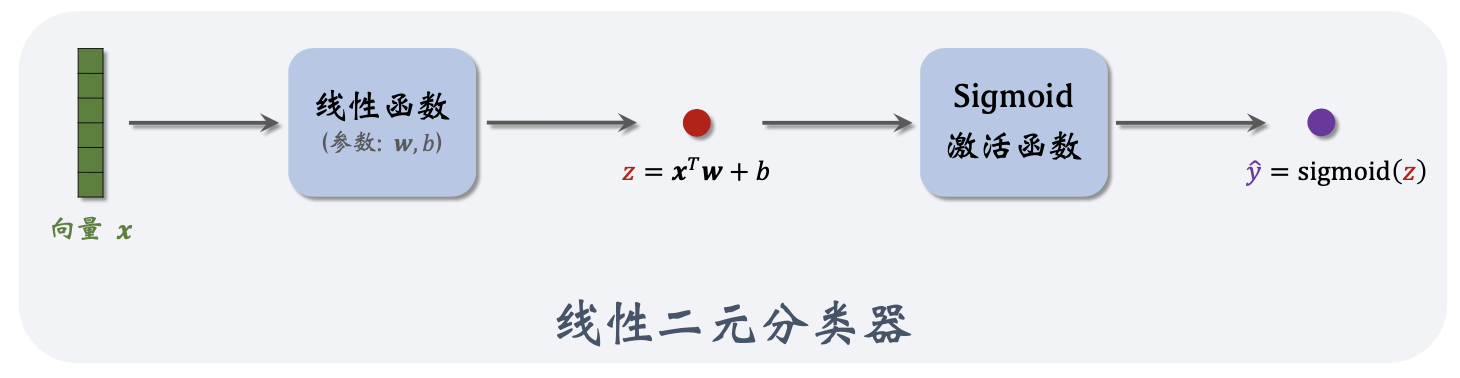
\includegraphics[width=0.5\linewidth]{ch4/figs/logistic_struction.png}
    \caption{逻辑回归,线性 Sigmoid 分类器的结构}
    \label{fig:logistic_struction}
\end{figure}

sigmoid 函数定义为:

\begin{equation}
    % \label{eq:softmax_act}$
    sigmoid(z) = \frac{1}{1+exp(-z)}
\end{equation}

如\figref{fig:sigmoid}所示,sigmoid 函数可以将输入的任意实数映射到$0-1$之间,对其输出的值进行判断,例如小于0.5我们认为预测的是类别0,反之是类别1,这样一来通过梯度下降来求解模型参数就可以用于实现二分类问题了。注意,虽然逻辑回归只是在线性回归模型基础上增加了一个激活函数,但两个模型是完全不同的,包括损失函数等等。线性回归的损失函数是均方差损失,而逻辑回归模型一般是交叉熵损失,这两种损失函数在深度学习和深度强化学习中都很常见,具体推导细节读者可自行翻阅相关资料。

\begin{figure}[hbt]
    \centering
    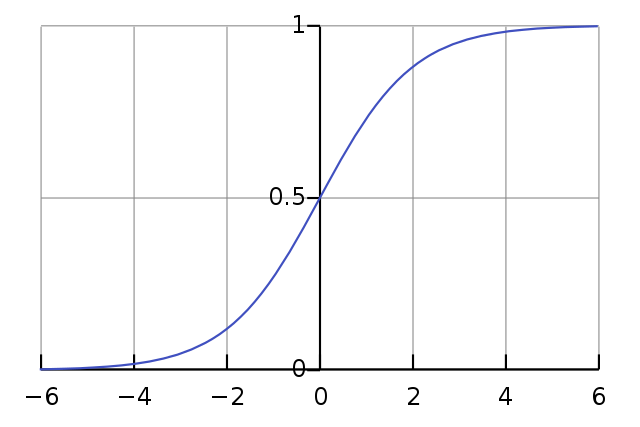
\includegraphics[width=0.5\linewidth]{ch4/figs/sigmoid.png}
    \caption{Sigmoid函数图像}
    \label{fig:sigmoid}
\end{figure}

\subsubsection{神经网络}

{\bfseries 全连接网络。} 全连接网络又称作多层感知机(multi-layer perceptron,MLP),是最基础的神经网络模型。它是基于生物神经网络的启发,将“线性函数+激活函数”这样的结构一层层堆叠(stack)组合成一个多层的网络模型,用于解决更复杂的问题。如\figref{fig:ann_vs_dnn}所示,线性函数可以看做生物神经网络的神经元,而激活函数就是神经元之间的突触结构。顺便说一句,生物神经网络是神奇且复杂的,人们也一直在尝试研究新的人工神经网络模型去模拟生物神经网络,例如脉冲神经网络,尽管目前这些模型还没有得到广泛地验证。

\begin{figure}[hbt]
    \centering
    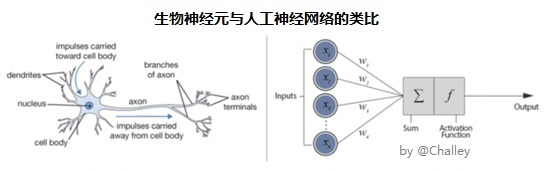
\includegraphics[width=0.5\linewidth]{ch4/figs/ann_vs_dnn.png}
    \caption{生物神经网络与人工神经网络的对比}
    \label{fig:ann_vs_dnn}
\end{figure}

记神经网络模型中上一层的输入向量为$\boldsymbol{x^{l-1}}\in \mathbb{R}^{d^{l-1}}$,其中第一层的输入也就是整个模型的输入可记为$\boldsymbol{x^0}$,每一个全连接层将上一层的输入映射到$\boldsymbol{x^{l}}\in \mathbb{R}^{d^{l}}$,也就是下一层的输入,具体定义为:

\begin{equation}
    \boldsymbol{x}^{l}=\sigma(\boldsymbol{z}), \quad \boldsymbol{z}=\boldsymbol{W} \boldsymbol{x^{l-1}}+\boldsymbol{b} = \boldsymbol{\theta} \boldsymbol{x^{l-1}}
\end{equation}

其中$\boldsymbol{W}\in \mathbb{R}^{d^{l-1} \times d^{l}}$是权重矩阵,$\boldsymbol{b}$为偏置矩阵,与线性模型类型,这两个参数我们通常看作一个参数$\boldsymbol{\theta}$。$\sigma(\cdot)$是激活函数,除了 Sigmoid 函数之外,还包括 Softmax 函数、ReLU 函数和 tanh 函数等等激活函数。其中最常用的是 ReLU 函数 和 tanh 函数,前者将神经元也就是线性函数的输出映射到$0-1$之间,后者则映射到$-1$到$1$之间。前面讲到,在强化学习中我们用神经网络来近似动作价值函数,动作价值函数的输入是状态,输出是各个动作对应的价值,在有些连续动作问题中比如汽车方向盘转动角度是$-90$度到$90$度之间,这种情况下使用 tanh 激活函数能够使得神经网络负值以便于更好地近似状态动作函数。顺便提一句,这里还有一种做法是我们可以把动作空间映射到正值的范围,例如$0$到$180$区间,这样一来对应的神经网络模型激活函数使用 ReLU 函数会更好些。

一个$l$层的神经网络模型可以表示为:
\begin{equation}
    \begin{split}
    第 1 层: \quad \boldsymbol{x}^{(1)}=\sigma_1\left(\boldsymbol{W}^{(1)} \boldsymbol{x}^{(0)}+\boldsymbol{b}^{(1)}\right),\\
    第 2 层: \quad \boldsymbol{x}^{(2)}=\sigma_2\left(\boldsymbol{W}^{(2)} \boldsymbol{x}^{(1)}+\boldsymbol{b}^{(2)}\right),\\
    \vdots \quad \vdots\\
    第 l 层: \quad \boldsymbol{x}^{(l)}=\sigma_l\left(\boldsymbol{W}^{(l)} \boldsymbol{x}^{(l-1)}+\boldsymbol{b}^{(l)}\right)\\
\end{split}
\end{equation}

求解神经网络模型参数的方法除了梯度下降之外,还涉及多层网络模型的正向传播和反向传播,具体细节在接下来的小节中展开。

{\bfseries 卷积神经网络。}

{\bfseries 循环神经网络。}


{\bfseries Transformer。}
\subsubsection{梯度下降}

TODO
\subsubsection{反向传播}
TODO
\subsection{ DQN 算法}

DQN 算法,英文全称 Deep Q-learning,顾名思义就是基于深度网络模型的 Q-learning 算法,主要由 DeepMind 公司于2013年和2015年分别提出的两篇论文来实现,即《Playing Atari with Deep Reinforcement Learning》和《Human-level Control through Deep Reinforcement Learning》。DQN 算法相对于 Q-learning 算法来说更新方法本质上是一样的,而 DQN 算法最重要的贡献之一就是本章节开头讲的,用神经网络替换表格的形式来近似动作价值函数$Q(\boldsymbol{s},\boldsymbol{a})$。

\begin{figure}[hbt]
    \centering
    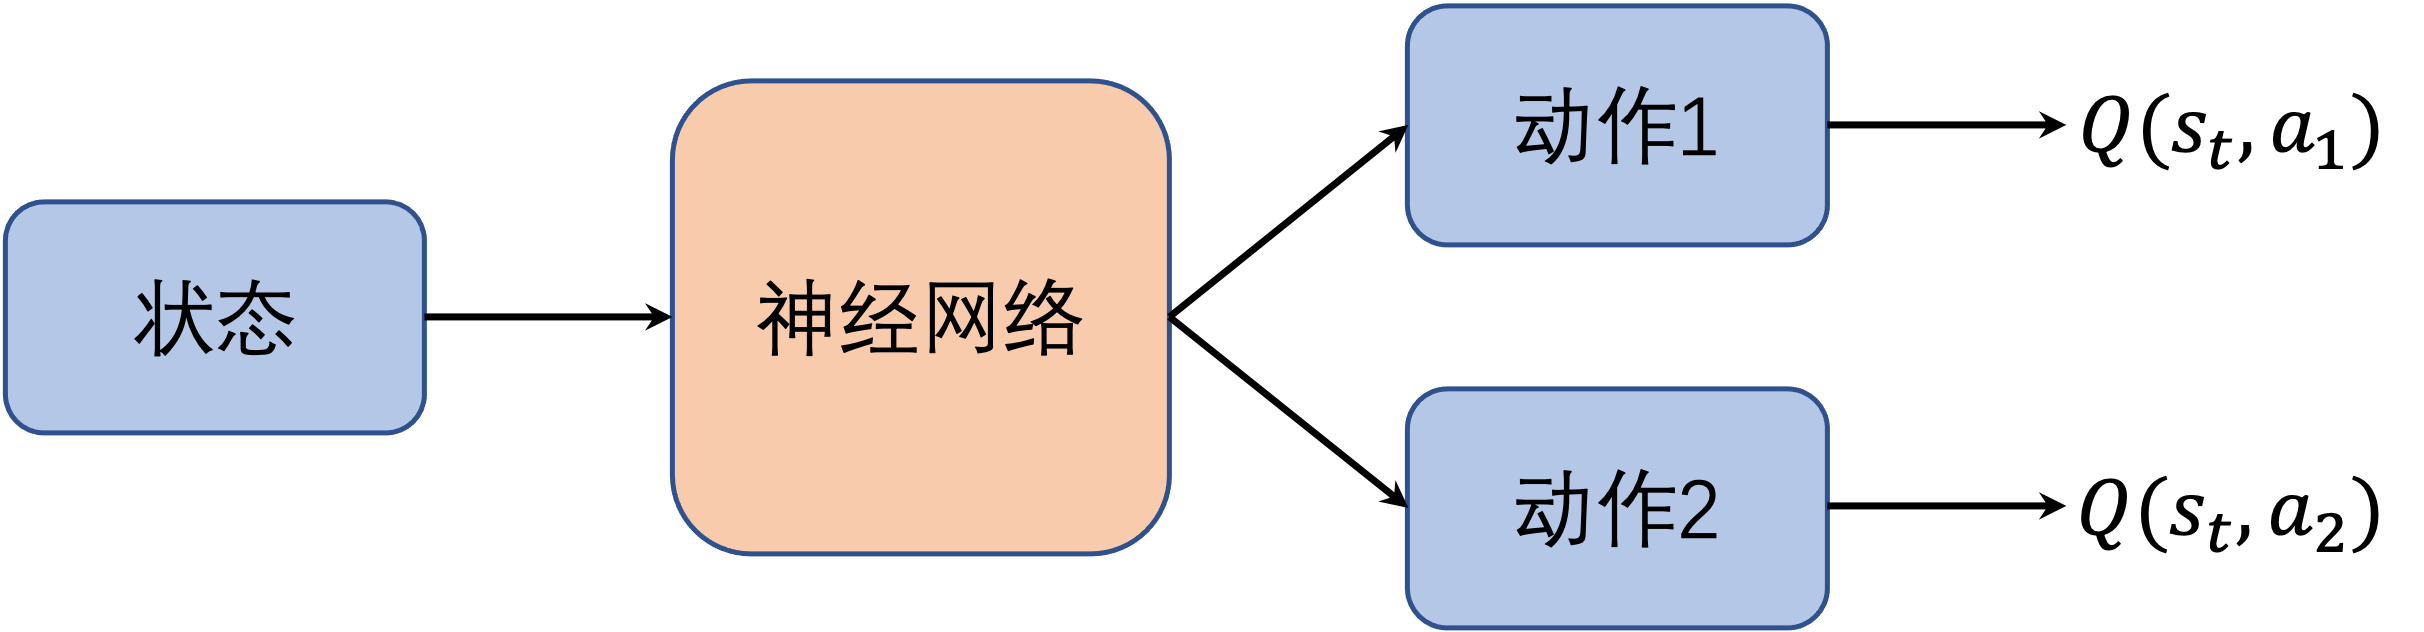
\includegraphics[width=0.5\linewidth]{ch4/figs/dqn_network.png}
    \caption{DQN 网络结构}
    \label{fig:dqn_network}
\end{figure}

如\figref{fig:dqn_network}所示,在 DQN 的网络模型中,我们将当前状态$s_t$作为输入,并输出动作空间中所有动作(假设这里只有两个动作,即1和2)对应的动作价值即$Q$值,我们记做$Q(s_t,\boldsymbol{a})$。对于其他状态,该网络模型同样可以输出所有动作对应的价值,这样一来神经网络近似的动作价值函数可以表示为$Q^{\theta}(\boldsymbol{s},\boldsymbol{a})$。其中$\theta$就是神经网络模型的参数,可以结合梯度下降的方法求解。

具体该怎么结合梯度下降来更新$Q$值呢?我们首先回顾一下 Q-learning 算法的更新公式如下:

\begin{equation}
    Q(s_t,a_t) \leftarrow Q(s_t,a_t)+\alpha[r_t+\gamma\max _{a}Q(s_{t+1},a)-Q(s_t,a_t)]
\end{equation}

我们注意到公式右边两项$r_t+\gamma\max _{a}Q(s_{t+1},a)$和$Q(s_t,a_t)$分别表示期望的$Q$值和实际的$Q$值,其中预测的$Q$值是用下一个状态对应$Q$值的最大值来近似的。换句话说,在更新$Q$值并达到收敛的过程中,期望的$Q$值也应该接近实际的$Q$值,即我们希望最小化$r_t+\gamma\max _{a}Q(s_{t+1},a)$和$Q(s_t,a_t)$之间的损失,其中$\alpha$是学习率,尽管优化参数的公式跟深度学习中梯度下降法优化参数的公式有一些区别(比如增加了$\gamma$和$r_t$等参数)。从这个角度上来看,强化学习跟深度学习的训练方式其实是一样的,不同的地方在于强化学习用于训练的样本(包括状态、动作和奖励等等)是与环境实时交互得到的,而深度学习则是事先准备好的训练集。当然训练方式类似并不代表强化学习和深度学习之间的区别就很小,本质上来说强化学习和深度学习解决的问题是完全不同的,前者用于解决序列决策问题,后者用于解决静态问题例如回归、分类、识别等等。在 Q-learning 中,我们是直接优化 Q 值的,而在 DQN 中使用神经网络来近似 Q 值,我们则需要优化网络模型对应的参数$\theta$,如下

\begin{equation}
    \begin{split}
    y_{i}= \begin{cases}r_{i} & \text {对于终止状态} s_{i} \\ r_{i}+\gamma \max _{a^{\prime}} Q\left(s_{i+1}, a^{\prime} ; \theta\right) & \text {对于非终止状态} s_{i}\end{cases}\\
    L(\theta)=\left(y_{i}-Q\left(s_{i}, a_{i} ; \theta\right)\right)^{2}\\
    \theta_i \leftarrow \theta_i - \alpha \nabla_{\theta_{i}} L_{i}\left(\theta_{i}\right)\\
\end{split}
\end{equation}

其中期望的Q值$y_{i}$增加了对终止状态和非终止状态的判断,这是因为当$s_t$为终止状态时,$Q(s_{t+1},a)$是不存在的($s_{t+1}$不存在),所以需要将其置0,在 Q-learning 中其实也需要有同样的操作,只是出于简化考虑没有列出。

\subsubsection{经验回放}

前面讲到,强化学习的训练方式是与环境实时交互得到样本然后进行训练的,在 Q-learning 中我们是每次交互一个样本,通常包含当前状态($state$)、当前动作($action$)、下一个状态($next\_state$)、是否为终止状态($done$),这样一个样本我们一般称之为一个状态转移(transition)。这种每次只交互一个样本并更新的方式会产生两个问题,首先是在强化学习问题中样本之间的关联性过强(从当前状态到下一个状态的过渡不可能是突变的,比如我们在吃饭时中间忽然加快速度张开血盆大口猛吃也不会导致我们的肚子一下子就鼓鼓的,会有一个相对缓慢的变化过程),会导致更新的过程不够稳定并且容易陷入局部最优解。本质上来说这其实就是随机梯度下降相对于单纯梯度下降的好处,只是在强化学习中体现得更为明显,因为强化学习前后两个样本的关联性往往比监督学习更紧密,从而导致训练的不稳定。另外一个问题是我们每次只看一个样本来更新,这在 DQN 算法中的劣势会更加明显,因为 DQN 算法是基于深度神经网络模型的。在深度学习的梯度下降中,我们知道如果在训练时每次遍历整个数据集并更新一次损失函数和梯度是会保证不错的收敛性的,但是计算开销会很大,这就是前面所说的批梯度下降方法(batch gradient descent)。但如果每次只看一个样本并更新梯度,尽管速度会提上去,但是会导致收敛性能不好,容易在最优点附近徘徊,于是有了一个折中的方法,即小批量梯度下降(mini-batch gradient descent)。鉴于这两个问题, DeepMind 公司 在论文中提出了一个经验回放的概念(replay buffer),这个经验回放的功能主要包括三个方面。首先是能够缓存一定量的状态转移即样本,此时 DQN 算法并不急着更新并累积一定的初始样本,就好比我们学习做饭炒菜一样,先把颠勺、抡刀、切菜、放调料等等都先零碎地试一遍。然后是每次更新的时候随机从经验回放中取出一个小批量的样本并更新策略,注意这里的随机和小批量以便保证我们存储动作价值函数的网络模型是小批量随机梯度下降的。最后要保证经验回放是具有一定的容量限制的,太小了会导致收集到的样本具有一定的局限性,太大了会失去经验本身的意义。这就好比我们在做自我规划一样,往往会根据自身经验制定一个三年或者五年计划,如果制定的计划周期太长比如制定一个二十年计划是没有任何意义的,因为二十年间的变数太多会导致制定的计划失去效用。类似的经验回放太大容易导致智能体在更新策略时可能会使用一些比较久远的样本,根据马尔可夫过程的性质,太过久远的样本对于当前状态的参考意义不大,就好比我们制定一个二十年当上小学校长的计划,等到十年过去后发现我们中间有太多的变数而身不由己,这样一来当初制定的二十年计划大概率就流产了。而小批量的样本更新就好比在三五年计划的基础上我们制定一个每周计划,每周行动并反思然后结合三五年计划或目标调整下一周的行动,这种方式往往是最高效的。到这里,我们又不得不感叹一句,生活中处处是强化学习!
\subsubsection{目标网络}

在 DQN 算法中还有一个重要的技巧,就是使用了一个每隔若干步才更新的目标网络,与之相对的,会有一个每步更新的网络,即每次从经验回放中采样到样本就更新网络参数,在本书中一般称之为策略网络。策略网络和目标网络结构都是相同的,都用于近似 Q 值,在实践中每隔若干步才把每步更新的策略网络参数复制给目标网络,这样做的好处是保证训练的稳定,避免 Q值 的估计发散。举一个典型的例子,这里的目标网络好比明朝的皇帝,而策略网络相当于皇帝手下的太监,每次皇帝在做一些行政决策时往往不急着下定论,会让太监们去收集一圈情报,然后集思广益再做决策。这样做的好处是显而易见的,比如皇帝要处决一个可能受冤的犯人时,如果一个太监收集到一个情报说这个犯人就是真凶的时候,如果皇帝是一个急性子可能就当初处决了,但如果这时候另外一个太监收集了一个更有力的证据证明刚才那个太监收集到的情报不可靠并能够证明该犯人无罪时,那么此时皇帝就已经犯下了一个无法挽回的过错。换句话说,如果当前有个小批量样本导致模型对 Q 值进行了较差的过估计,如果接下来从经验回放中提取到的样本正好连续几个都这样的,很有可能导致 Q 值的发散(它的青春小鸟一去不回来了)。再打个比方,我们玩 RPG 或者闯关类游戏,有些人为了破纪录经常存档(Save)和回档(Load),简称“SL”大法。只要我出了错,我不满意我就加载之前的存档,假设不允许加载呢,就像 DQN 算法一样训练过程中会退不了,这时候是不是搞两个档,一个档每帧都存一下,另外一个档打了不错的结果再存,也就是若干个间隔再存一下,到最后用间隔若干步数再存的档一般都比每帧都存的档好些呢。当然我们也可以再搞更多个档,也就是DQN增加多个目标网络,但是对于 DQN 算法来说没有多大必要,因为多几个网络效果不见得会好很多。


\subsubsection{探索策略}
\subsection{实战:DQN算法}


\subsection{关键词}
\subsection{习题}
\subsection{面试题}
\subsection{本章小结}
    % \section{策略梯度}
本章开始介绍基于策略梯度(policy based)的算法,与前面介绍的基于价值(value based)的算法(包括Q learning,SARSA以及DQN等等)不同,这类算法直接对策略本身进行近似优化。在这种情况下,我们可以将策略描述成一个带有参数$\theta$的连续函数,该函数将某个状态作为输入,输出的不再是某个确定性(deterministic)的离散动作,而是对应的动作概率分布,通常用$\pi_{\theta}(a|s)$表示,称作随机性(stochastic)策略。下面我们将从最基本的策略梯度算法展开。

\subsection{策略梯度算法}

尽管策略梯度算法是将策略参数化成一个连续的函数$\pi_{\theta}(a|s)$,但是与基于价值的算法本质上是一样的,最终的优化目标都是累积的价值期望$V^{*}(s)$。例如在前面章节的 Q learning 算法中,我们利用贝尔曼方程求解马尔科夫决策过程中的最佳决策序列,进而求出对应的最优动作价值函数$Q^{*}(s,a)$,不清楚的读者可以再回到前面的内容温习一下。

策略一般记作 $\pi$。假设我们使用深度学习来做强化学习,策略就是一个网络。网络里面有一些参数,我们用 $\theta$ 来代表 $\pi$ 的参数。
网络的输入是智能体看到的东西,如果让智能体玩视频游戏,智能体看到的东西就是游戏的画面。智能体看到的东西会影响我们训练的效果。例如,在玩游戏的时候, 也许我们觉得游戏的画面是前后相关的,所以应该让策略去看从游戏开始到当前这个时间点之间所有画面的总和。因此我们可能会觉得要用到循环神经网络(recurrent neural network,RNN)来处理它,不过这样会比较难处理。
我们可以用向量或矩阵来表示智能体的观测,并将观测输入策略网络,策略网络就会输出智能体要采取的动作。
\figref{fig:actor_policy} 就是具体的例子,策略是一个网络;输入是游戏的画面,它通常是由像素组成的;输出是我们可以执行的动作,有几个动作,输出层就有几个神经元。假设我们现在可以执行的动作有 3 个,输出层就有 3 个神经元,每个神经元对应一个可以采取的动作。输入一个东西后,网络会给每一个可以采取的动作一个分数。我们可以把这个分数当作概率,演员根据概率的分布来决定它要采取的动作,比如 0.7 的概率向左走、0.2 的概率向右走、0.1的概率开火等。概率分布不同,演员采取的动作就会不一样。

\begin{figure}[hbt]
    \centering
    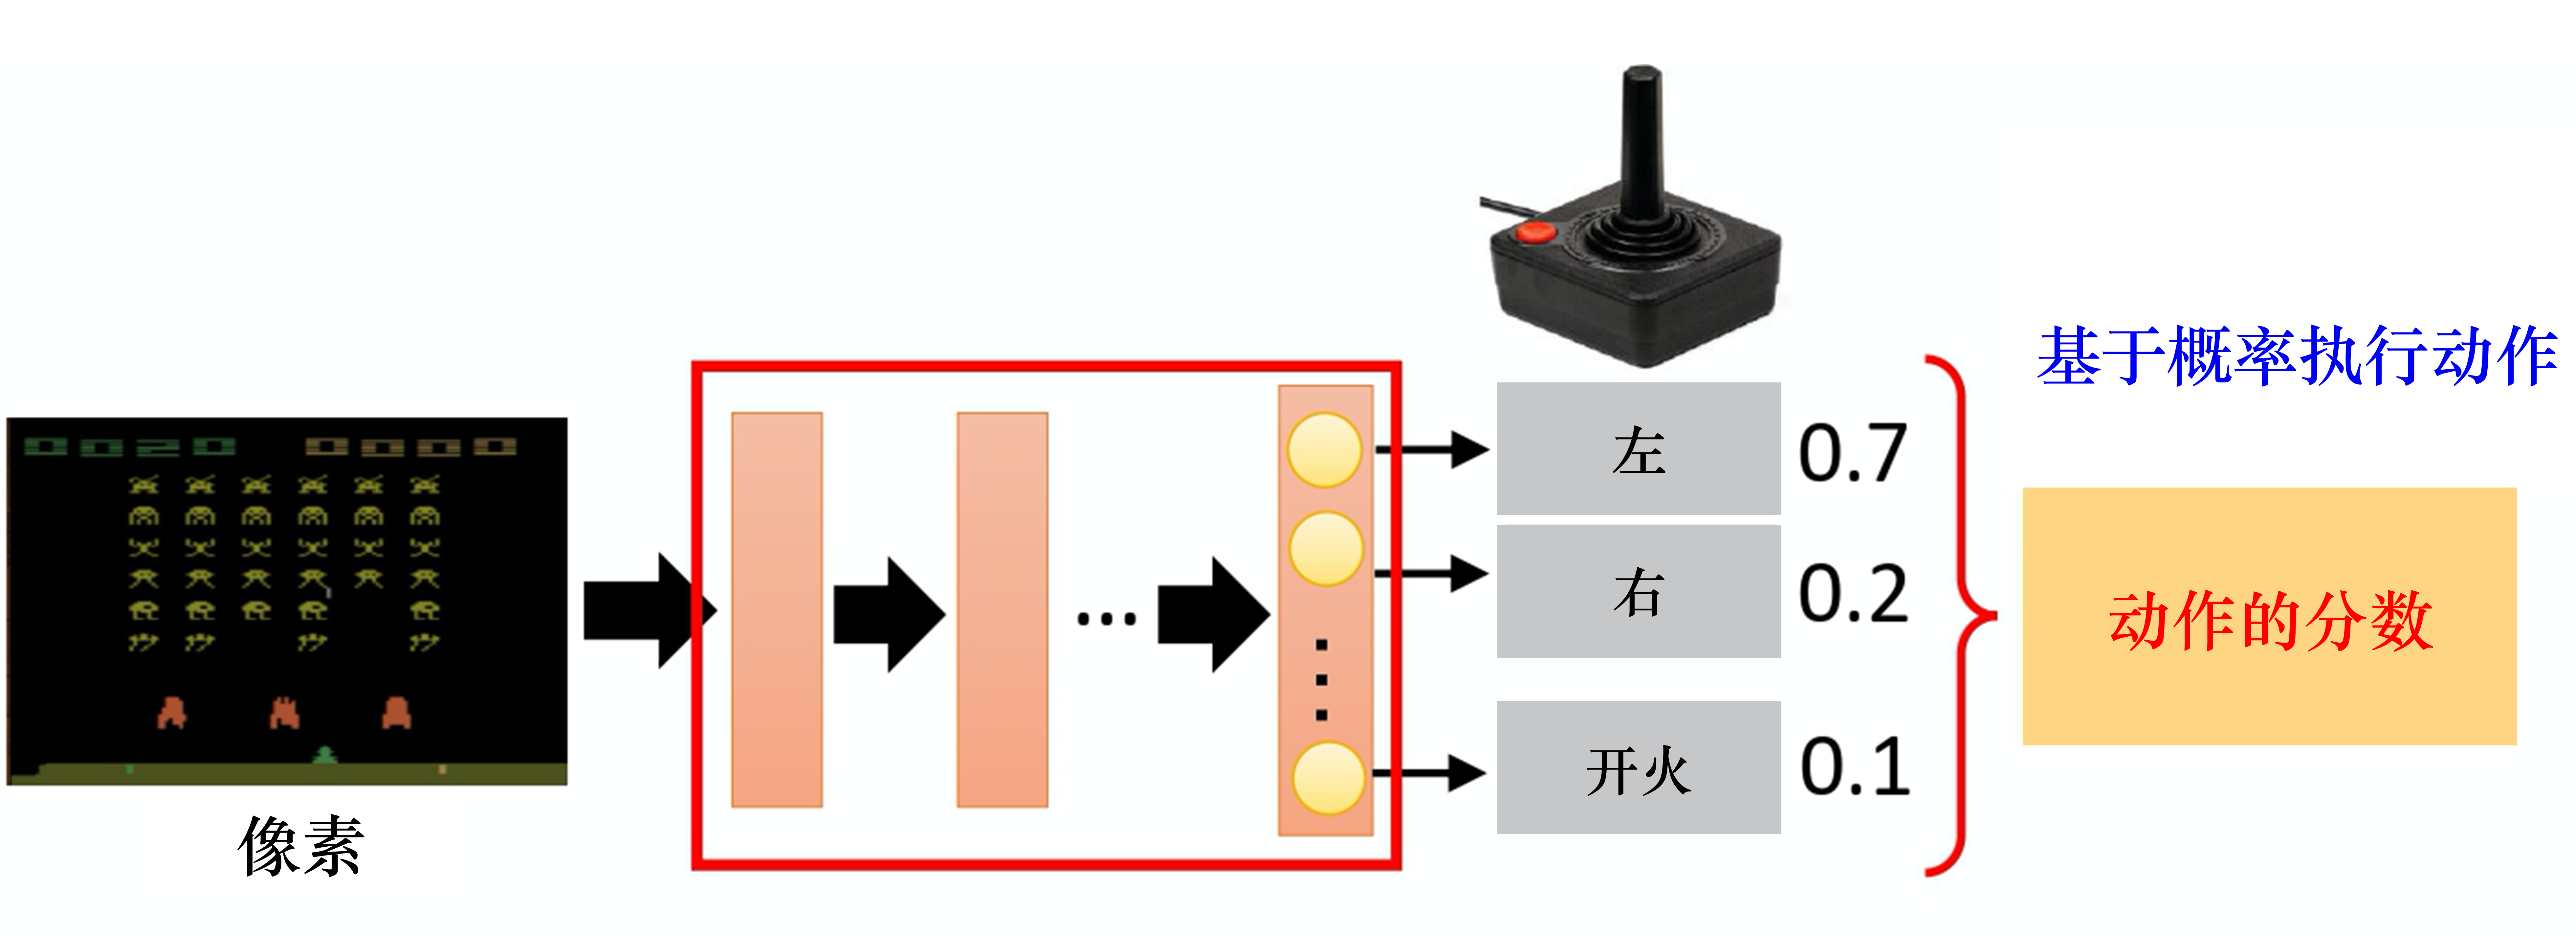
\includegraphics[width=0.5\linewidth]{ch6/figs/actor_policy.png}
    \caption{演员的策略}
    \label{fig:actor_policy}
\end{figure}

接下来我们用一个例子来说明演员与环境交互的过程。

如\figref{fig:example_play_game}所示,首先演员会看到一个视频游戏的初始画面,接下来它会根据内部的网络(内部的策略)来决定一个动作。假设演员现在决定的动作是向右,决定完动作以后,它就会得到一个奖励,奖励代表它采取这个动作以后得到的分数。

我们把游戏初始的画面记作 $s_0$, 把第一次执行的动作记作 $a_0$,把第一次执行动作以后得到的奖励记作 $r_1$。
这里不同的人有不同的记法,有人觉得应该从 $s_1$ 开始,并且执行 $a_1$ 得到的奖励应该记为 $r_1$,这两种记法都可以。只是一般来说,是智能体先做出动作,然后环境再输出奖励和新的状态,也就是说这个新的状态和奖励应该对应着同一时刻,也就是同一下标。我们通常喜欢从 0 时刻开始记录轨迹,此轨迹可以将交互过程清晰地体现出来。
演员决定一个动作以后,就会看到一个新的游戏画面$s_1$。把 $s_1$ 输入给演员,演员决定要开火,它可能打败了一只怪兽,就得到五分。这个过程反复地持续下去,直到在某一个时间点执行某一个动作,得到奖励之后,环境决定这个游戏结束。例如,如果在这个游戏里面,我们控制宇宙飞船去击杀怪兽,如果宇宙飞船被毁或是把所有的怪兽都清空,游戏就结束了。

\begin{figure}[hbt]
    \centering
    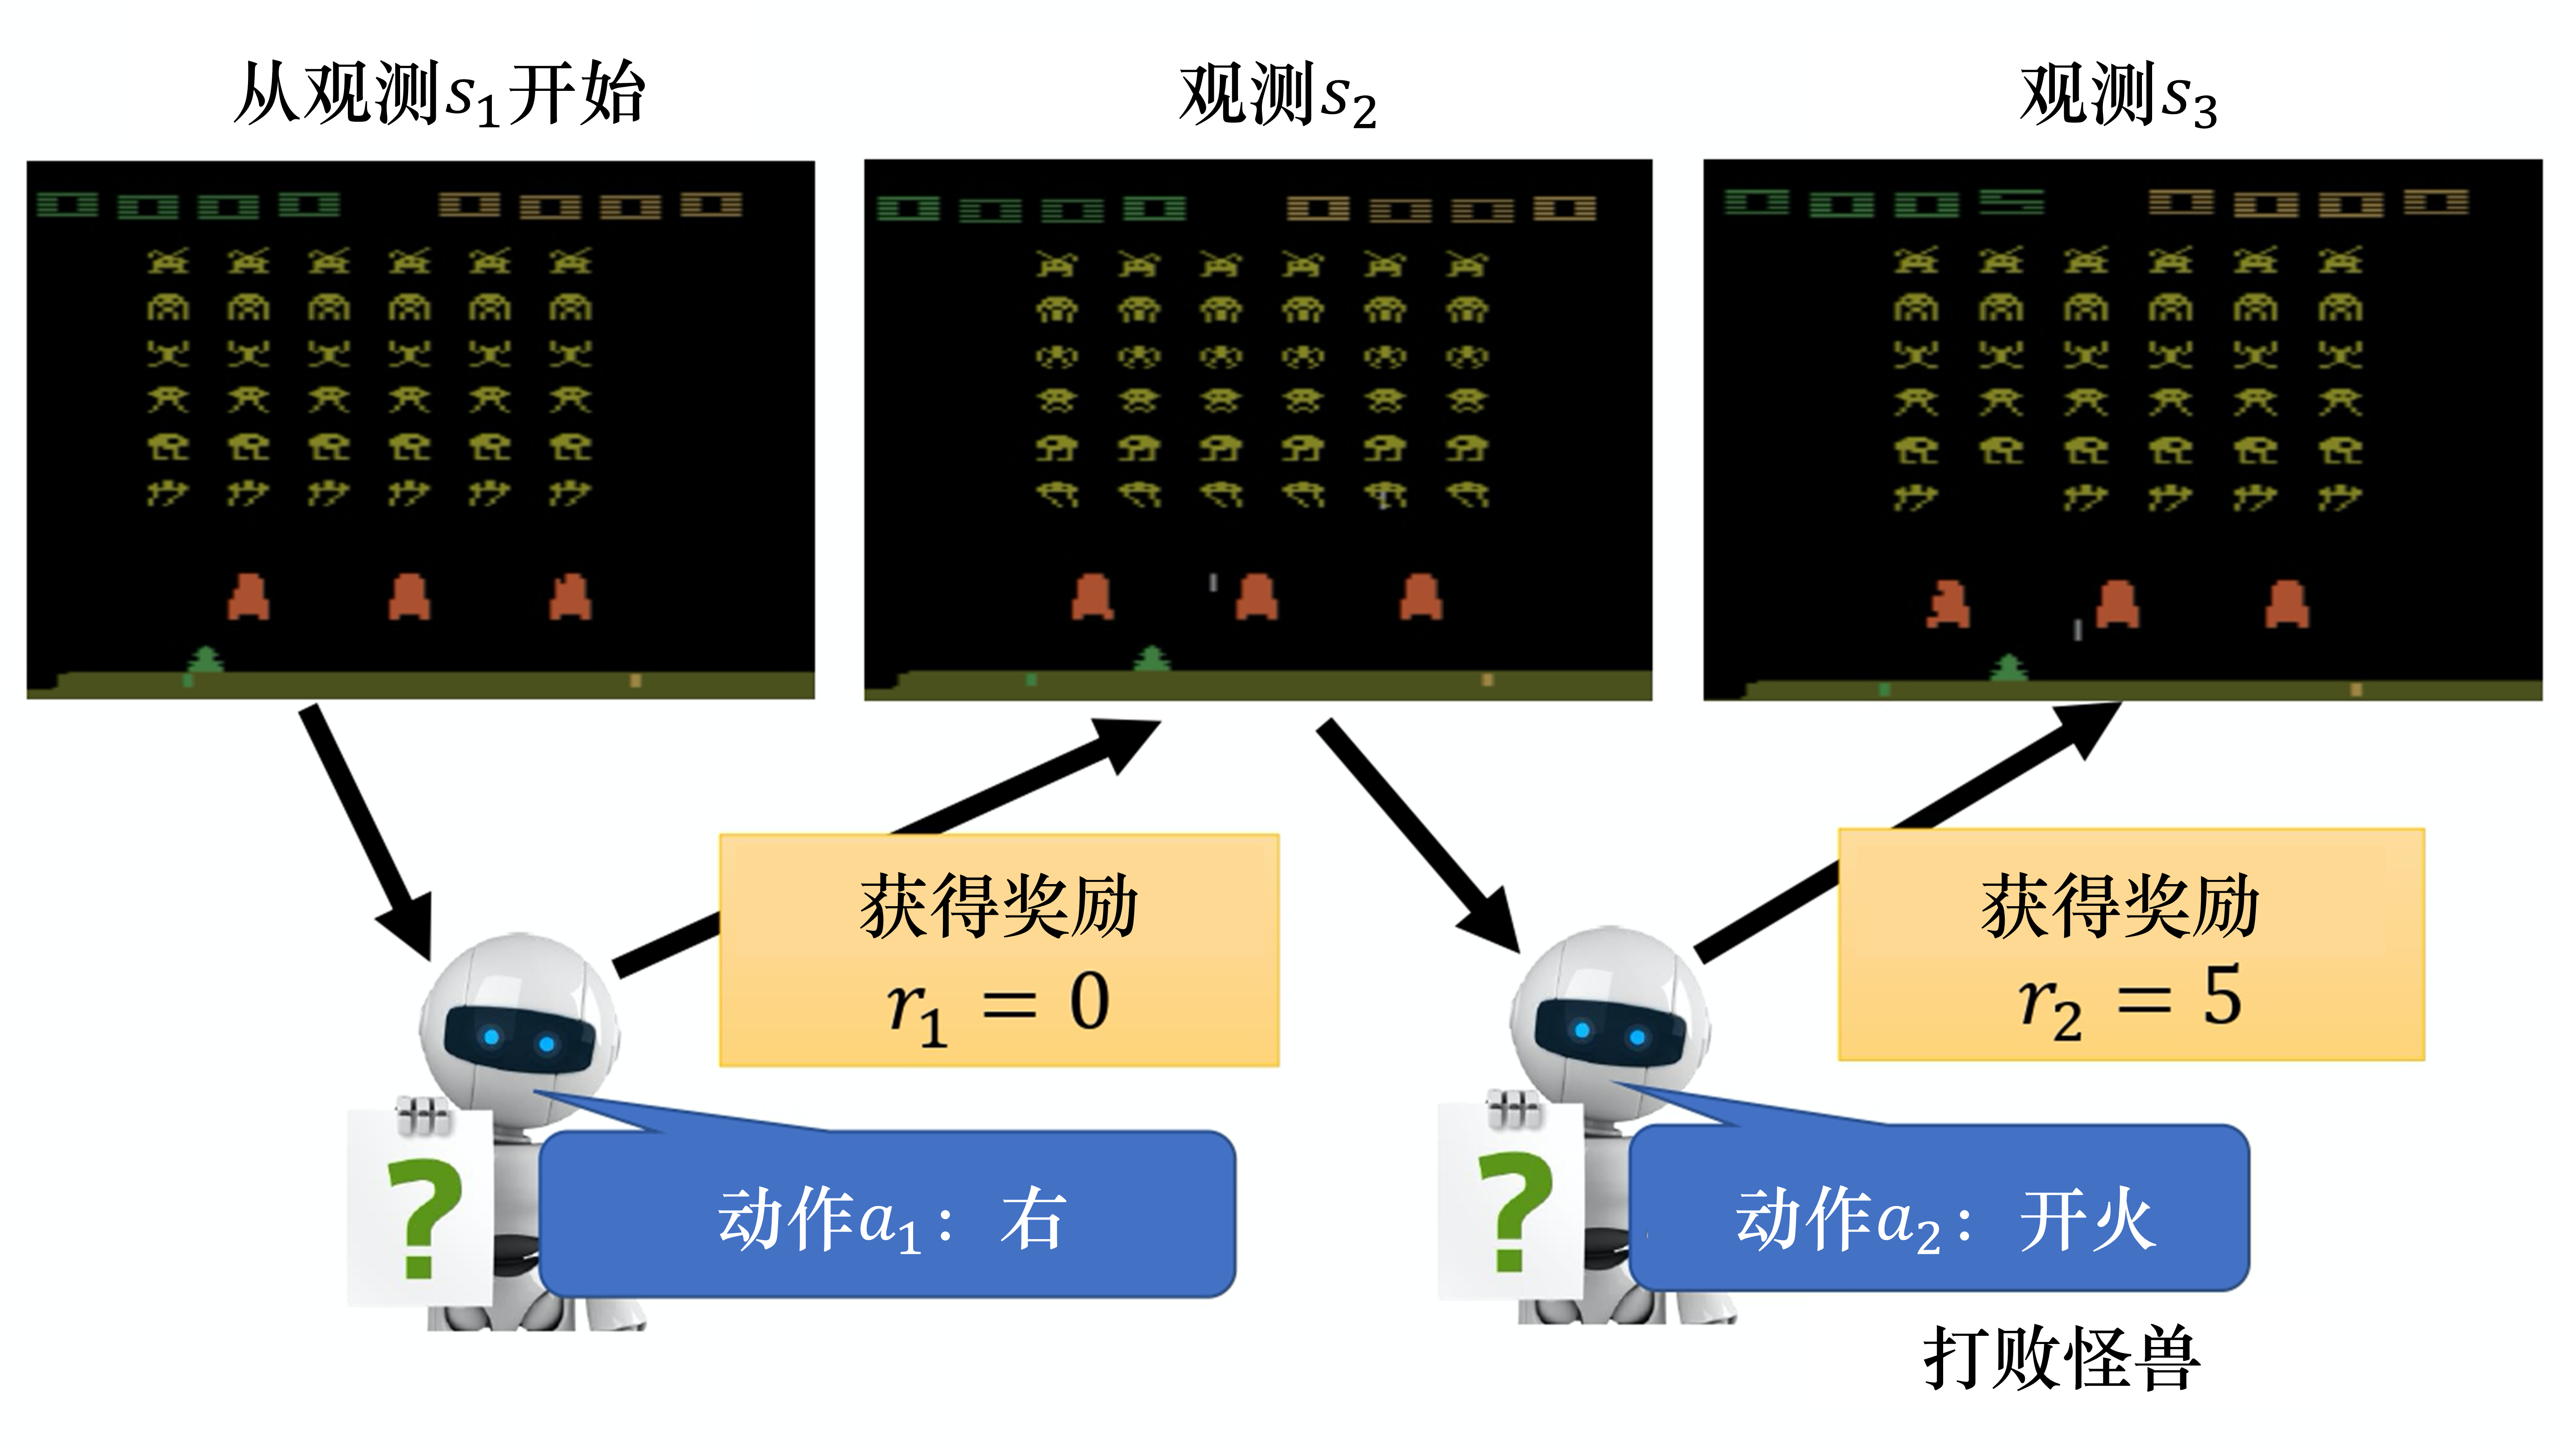
\includegraphics[width=0.5\linewidth]{ch6/figs/example_play_game.png}
    \caption{玩视频游戏的例子}
    \label{fig:example_play_game}
\end{figure}


那么在策略梯度算法中我们怎样去推导出最优策略下的价值期望呢?首先我们知道强化学习解决的问题基本上都可以被描述为马尔可夫决策过程,而马尔可夫决策过程同时也是成环境与智能体不断交互的过程,即环境与策略不断交互的过程,因为智能体是策略的载体。如\figref{fig:env_agent} 所示,环境首先“吐”出一个初始状态$s_0$,然后智能体观测到状态$s_0$,它会“吐”出相应的动作 $a_0$。紧接着环境接收到 $a_0$ 反馈出新的状态 $s_1$,然后智能体观测到新的状态继续采取新的动作......如此循环往复,直到满足环境的停止条件为止。

\begin{figure}[hbt]
    \centering
    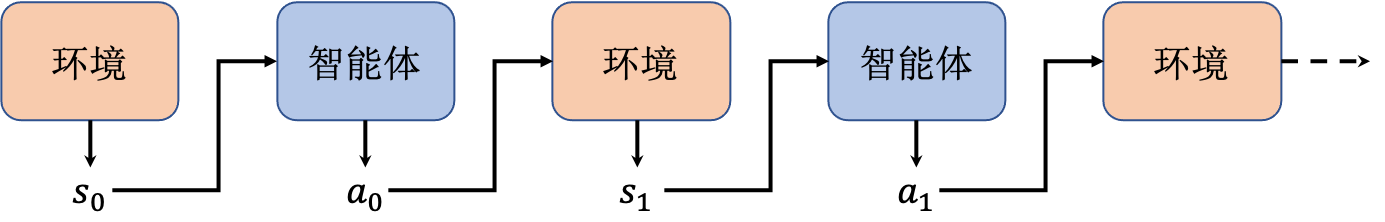
\includegraphics[width=0.5\linewidth]{ch6/figs/env_agent.png}
    \caption{智能体与环境}
    \label{fig:env_agent}
\end{figure}

在这样一个过程之后,我们把环境输出的所有状态 $s$ 与智能体输出的对应动作 $a$ 全部组合起来,就形成了一条轨迹(trajectory),即
\begin{equation}
    \label{eq:}
    \tau=\left\{s_{0}, a_{0}, s_{1}, a_{1}, \cdots, s_{t}, a_{t}\right\}
\end{equation}

这里环境也可以看作一个函数,我们设在给定状态$s_t$和动作$a_t$的情况下,它“吐”出状态$s_{t+1}$的概率为$p(s_{t+1} | s_{t}, a_{t})$,即是马尔可夫决策过程中的转移概率。此外我们假设环境以一个概率$p(s_{0})$“吐”出初始状态,在给定策略函数$\pi_{\theta}(a|s)$的情况下,我们就可以计算某个轨迹$\tau$发生的概率为
\begin{equation}
    \label{eq:station_dist}
    \begin{aligned}
        P_{\theta}(\tau)
        &=p(s_{0}) \pi_{\theta}(a_{0} | s_{0}) p(s_{1} | s_{0}, a_{0}) \pi_{\theta}(a_{1} | s_{1}) p(s_{2} | s_{1}, a_{1}) \cdots \\
        &=p(s_{0}) \prod_{t=0}^{T} \pi_{\theta}\left(a_{t} | s_{t}\right) p\left(s_{t+1} | s_{t}, a_{t}\right)
    \end{aligned}
\end{equation}

也就是说我们先计算环境输出初始状态 $s_0$ 的概率 $p(s_0)$,再计算智能体根据 $s_0$ 动作执行 $a_0$ 的概率,也就是策略函数$p_{\theta}\left(a_{0} | s_{0}\right)$。然后环境结合当前状态$s_0$根据动作$a_0$以一定的概率反馈出新的状态 $s_1$,也就是转移概率$p(s_{1} | s_{0}, a_{0})$。 
这样的转移概率通常情况下是一定存在的,也就是不为0,因为 $s_1$ 与 $s_0$ 一般说来是有关系的。举个例子,我们玩电脑游戏时,一般都是根据每一帧的游戏画面给出的信息来采取我们认为的最优动作以便于获得游戏的最终胜利。这种情况下,游戏画面可以看作状态,比如当前帧画面为$s_0$,下一帧画面就是 $s_1$ 。由于游戏画面是连续的,因此下一帧游戏画面$s_1$ 与上一帧游戏画面$s_0$ 通常是有联系的。如果显示器输出游戏画面的时候没有概率,极端情况下游戏的画面就会始终停留在某一帧下,此时我们只要找到一条路径就可以过关了,这样的游戏就没有意义。所以输出游戏画面时通常有一定概率,给定同样的前一个画面,我们采取同样的动作,下次产生的画面不一定是一样的。如此反复执行下去,我们就可以计算出一条轨迹 $\tau$ 出现的概率了。

前面讲到,无论是基于价值还是基于策略梯度的方法,我们的目标都是希望最终累积的价值期望最大,这个价值的定义或者说近似也是比较多样的,可以是简单的累积奖励之和,也可以是包含折扣因子$\gamma$的累积奖励之和,也就是通常我们所说的回报$G$(return)。如何近似这个价值期望也是研究者们近年来一直在不断地优化策略梯度算法的重点之一,这个在后面章节我们讲A2C和GAE等算法的时候会继续展开,现在我们姑且将这个价值近似为最为简单的累积奖励。

再简单回顾一下马尔可夫决策过程。我们知道强化学习中除了智能体和环境之外,还会涉及奖励。奖励一般是由环境反馈得到的,如\figref{fig:expected_reward} 所示,环境根据在某个状态以及在这一状态下智能体采取的某个动作来决定这个动作可以得到的分数,也就是奖励。例如,输入$s_0$、$a_0$,它会输出$r_1$;输入 $s_1$、$a_1$,会输出 $r_2$ 等等,如\eqref{eq:traj_reward}。

\begin{equation}
    \label{eq:traj_reward}
    \tau=\left\{s_{0}, a_{0}, s_{1},r_{1},a_{1},\cdots, s_{t-1}, r_{t-1}, a_{t-1},s_{t},r_{t}\right\}
\end{equation}

\begin{figure}[hbt]
    \centering
    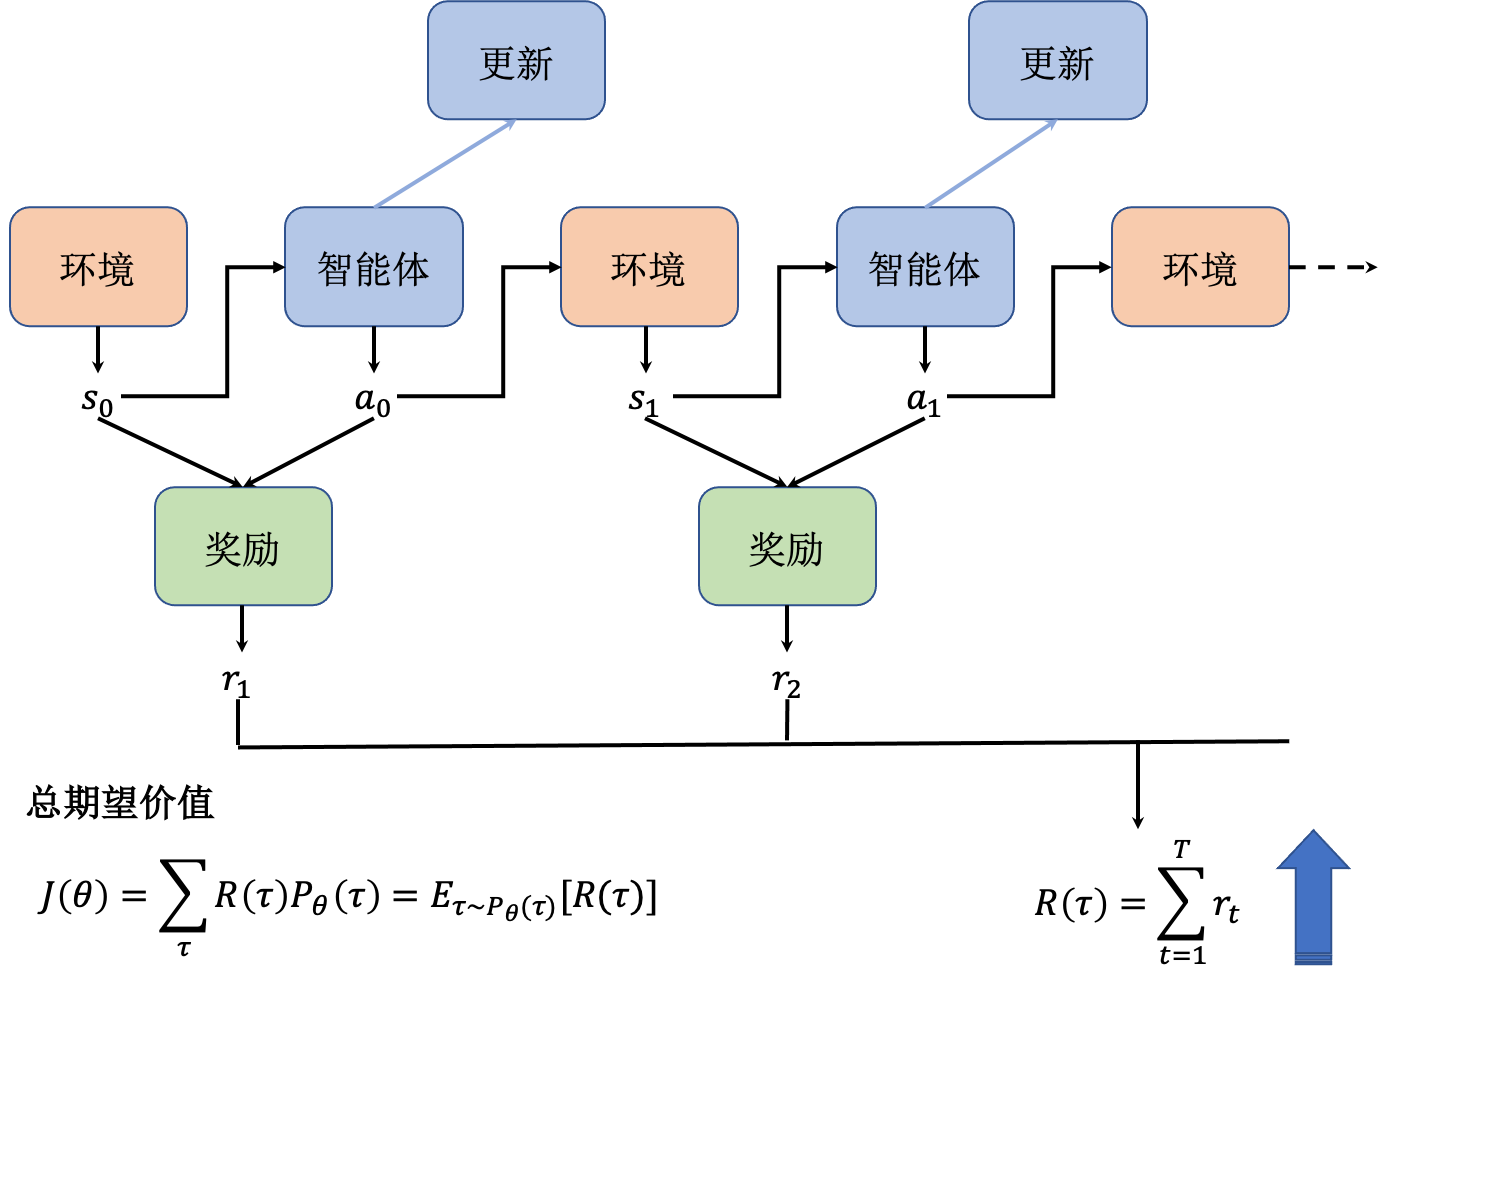
\includegraphics[width=0.5\linewidth]{ch6/figs/expected_reward.png}
    \caption{期望的奖励}
    \label{fig:expected_reward}
\end{figure}

奖励一般也可以近似成关于状态和动作的函数,即$r_{t+1}=r(s_t,a_t),t=0,1,\cdots$。对于一条轨迹$\tau$,我们可以计算其对应的累积奖励为$R(\tau)=\sum_{t=0}^T r\left(s_t, a_t\right)$。那么在给定的策略下,即参数$\theta$固定,对于不同的初始状态,会形成不同的轨迹$\tau_{1},\tau_{2},\cdots$,对应轨迹的出现概率前面已经推导出来为$P_{\theta}(\tau_{1}),P_{\theta}(\tau_{2}),\cdots$,累积奖励则为$R(\tau_{1}),R(\tau_{2}),\cdots$。回忆一下概率论中的全期望公式,是不是该策略的价值期望公式就可以通过每条轨迹的概率乘上对应的累积奖励再求和得到呢?答案是肯定的!如\eqref{eq:expect_policy},这就是我们所要找的目标函数。

\begin{equation}
    \label{eq:expect_policy}
    \begin{aligned}
    J(\pi_{\theta}) = P_{\theta}(\tau_{1})R(\tau_{1})+P_{\theta}(\tau_{2})R(\tau_{2})+\cdots \\
    &=\int_\tau P_{\theta}(\tau) R(\tau) \\ 
    &=E_{\tau \sim P_\theta(\tau)}[\sum_t r(s_t, a_t)] \\
    &=\underset{\tau \sim \pi_\theta}{E}[R(\tau)] 
    \end{aligned}
\end{equation}

有了目标函数,读者如果学过深度学习就会很自然地想到用梯度下降或者上升的方法来求解对应的最优参数$\theta^{*}$,这里需要用到梯度上升法,因为我们的目标是让总的累积价值期望$J(\pi_{\theta})$最大,而不是最小。当然我们也可以将目标函数取负号,即求解$-J(\pi_{\theta})$,然后再用梯度下降法去求解。梯度下降是更为普遍的做法,熟悉Tensorflow或者PyTorch等框架的读者应该比较清楚,这些框架默认的优化器设置就是梯度下降的,因此实际编程的时候如果我们的目标是最大化某个量,我们就会取这个量的相反数来优化。再比如用过scipy模块中的linprog函数来求解线性规划的读者也会知道,linprog函数默认的设置是求目标函数的最小值,而不是最大值,当我们的实际问题是求最大值时,我们也会进行取反的操作。

回归正题,梯度下降方法的关键还是在于求出$J(\pi_{\theta})=\int_\tau P_{\theta}(\tau) R(\tau)$的梯度,但是一眼看上去似乎不太好求。我们先不着急,首先我们是求关于参数$\theta$的梯度,可以看到$R(\tau)$跟$\theta$其实是没有关联的,因此在求解梯度的时候可以将这一项看作常数。那么接下来就是怎么求$P_{\theta}(\tau)$关于$\theta$的梯度了,我们需要用到一个对数微分的技巧,即$\log x$的导数是$1/x$。注意这里我们通常默认$\log$的底数是$e$,因此这里$\log x$也就是我们常见的$\ln x$,在大学数学之后的概念中我们通常是写作$\log x$,同学们请务必习惯。根据这个技巧,我们就可以推出\eqref{eq:log_trick}。
\begin{equation}
    \label{eq:log_trick}
    \nabla_\theta P_{\theta}(\tau)= P_{\theta}(\tau) \frac{\nabla_\theta P_{\theta}(\tau)}{P_{\theta}(\tau) }= P_{\theta}(\tau) \nabla_\theta \log P_{\theta}(\tau)
\end{equation}

现在的问题就从求$P_{\theta}(\tau)$的梯度变成了求$\log P_{\theta}(\tau)$的梯度了,即求$\nabla_\theta \log P_{\theta}(\tau)$。我们先求出$\log P_{\theta}(\tau)$,根据\eqref{eq:station_dist},$P_{\theta}(\tau)=p(s_{0}) \prod_{t=0}^{T} \pi_{\theta}\left(a_{t} | s_{t}\right) p\left(s_{t+1}  s_{t}, a_{t}\right)$,再根据对数公式$log (ab) = log a + log b$,即可求出:

\begin{equation}
    \label{eq:station_dist_log}
    \log P_{\theta}(\tau)= \log p(s_{0})  +  \sum_{t=0}^T(\log \pi_{\theta}(a_t \mid s_t)+\log p(s_{t+1} \mid s_t,a_t))
\end{equation}

我们惊奇地发现$\log P_{\theta}(\tau)$展开之后只有中间的项$\log \pi_{\theta}(a_t \mid s_t)$跟参数$\theta$有关,也就是说其他项关于$\theta$的梯度为0,如\eqref{eq:station_dist_log_grad}所示。
\begin{equation}
    \label{eq:station_dist_log_grad}
    \begin{aligned}
    \nabla_\theta \log P_{\theta}(\tau) &=\nabla_\theta \log \rho_0\left(s_0\right)+\sum_{t=0}^T\left(\nabla_\theta \log \pi_\theta\left(a_t \mid s_t\right)+\nabla_\theta \log p\left(s_{t+1} \mid s_t, a_t\right)\right) \\
    &=0+\sum_{t=0}^T\left(\nabla_\theta \log \pi_\theta\left(a_t \mid s_t\right)+0\right) \\
    &=\sum_{t=0}^T \nabla_\theta \log \pi_\theta\left(a_t \mid s_t\right)
    \end{aligned}
\end{equation}

现在我们就可以很方便地求出目标函数的梯度了,如\eqref{eq:pg_ob_grad}所示。

\begin{equation}
    \label{eq:pg_ob_grad}
    \begin{aligned}
    \nabla_\theta J\left(\pi_\theta\right) &=\nabla_\theta \underset{\tau \sim \pi_\theta}{\mathrm{E}}[R(\tau)] \\
    &=\nabla_\theta \int_\tau P_{\theta}(\tau) R(\tau) \\
    &=\int_\tau \nabla_\theta P_{\theta}(\tau) R(\tau) \\
    &=\int_\tau P_{\theta}(\tau) \nabla_\theta \log P_{\theta}(\tau) R(\tau) \\
    &=\underset{\tau \sim \pi_\theta}{\mathrm{E}}\left[\nabla_\theta \log P_{\theta}(\tau) R(\tau)\right]\\
    &= \underset{\tau \sim \pi_\theta}{\mathrm{E}}\left[\sum_{t=0}^T \nabla_\theta \log \pi_\theta\left(a_t \mid s_t\right) R(\tau)\right]
    \end{aligned}
\end{equation}

我们再简单解释一下\eqref{eq:pg_ob_grad}中的步骤,首先第一行就是目标函数的表达形式,到第二行就是全期望展开式,到第三行就是利用了积分的梯度性质,即梯度可以放到积分号的里面也就是被积函数中,第四行到最后就是对数微分技巧了。回过头来看下,我们为什么要用到对数微分技巧呢?这其实是一个常见的数学技巧:当我们看到公式中出现累乘的项时,我们通常都会取对数简化,因为根据对数公式的性质可以将累乘的项转换成累加的项,这样一来问题会更加便于处理。

我们可以直观地理解\eqref{eq:pg_ob_grad},即在采样到的数据里面,$(s_t,a_t)$ 可看作整个轨迹 $\tau$ 里面的某一个状态$-$动作对,假设我们在 $s_t$ 下执行 $a_t$时,最后发现 $\tau$ 的奖励是正的,我们就要增加在 $s_t$ 下执行 $a_t$ 的概率。反之,如果若 $\tau$ 的奖励是负的, 我们就要减少在 $s_t$ 下执行 $a_t$ 的概率,这其实就是梯度的思想。前面讲到我们将目标函数取反,就可以用梯度下降方法求取最优的参数$\theta$,即
\begin{equation}
    \label{eq:theta_update}
    \theta \leftarrow \theta - \alpha (-\nabla_\theta J\left(\pi_\theta\right))
\end{equation}
其中$\alpha$表示学习率,不明白\eqref{eq:theta_update}的读者就可以再去温习一下梯度下降法的原理,实际编程过程中我们还可以用 Adam、RMSProp 等方法来调整学习率,具体见后面的实战内容。

\subsection{REINFORCE算法}

在本小节中我们将介绍策略梯度中最简单也是最经典的一个算法\kw{REINFORCE},又称蒙特卡洛策略梯度算法(Monte Carlo Policy Gradient)。在介绍该算法之前,我们先回顾一下蒙特卡洛方法。

如\figref{fig:mc_td} 所示,蒙特卡洛方法可以理解为算法完成一个回合之后,再利用这个回合的数据去更新策略,也就是学习。因为我们已经获得了整个回合的数据,相应地也能够知道每一个步骤的奖励,我们可以很方便地计算每个步骤的未来总奖励,即回报 $G_t$。$G_t$ 是未来总奖励,代表从这个步骤开始,我们能获得的奖励之和。$G_1 $代表我们从第一步开始,往后能够获得的总奖励。$G_2$ 代表从第二步开始,往后能够获得的总奖励。

相比蒙特卡洛方法一个回合更新一次,时序差分方法是每个步骤更新一次,即每走一步,更新一次,时序差分方法的更新频率更高。时序差分方法使用Q函数来近似地表示未来总奖励 $G_t$。
\begin{figure}[hbt]
    \centering
    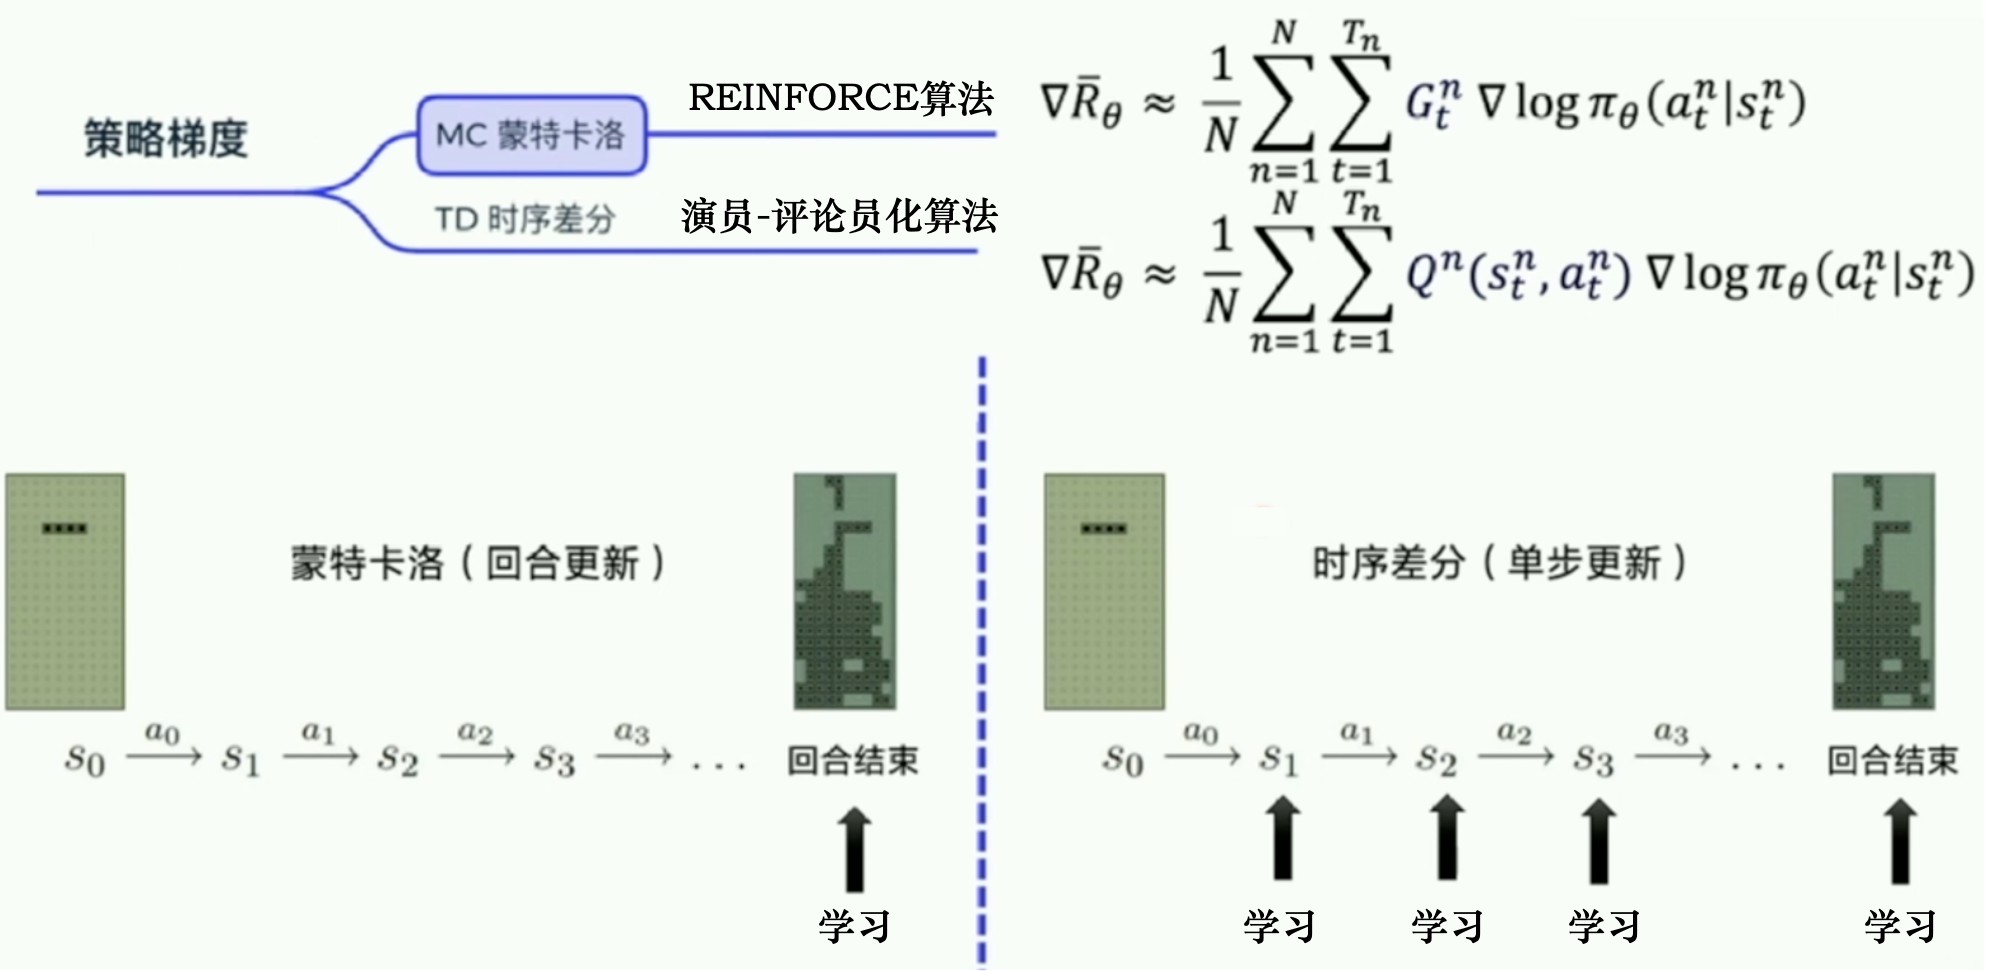
\includegraphics[width=0.5\linewidth]{ch6/figs/mc_td.png}
    \caption{蒙特卡洛方法与时序差分方法}
    \label{fig:mc_td}
\end{figure}

REINFORCE 算法正是利用蒙特卡洛算法来计算每回合生成的轨迹的价值,即$G_t$,然后乘上对应轨迹的概率从而计算总的价值期望,即\eqref{eq:reinforce_update}。

\begin{equation}
    \label{eq:reinforce_update}
    \nabla J_{\theta} \approx \frac{1}{N} \sum_{n=1}^{N} \sum_{t=1}^{T_{n}} G_{t}^{n} \nabla \log \pi_{\theta}\left(a_{t}^{n} \mid s_{t}^{n}\right)
\end{equation}

我们回顾一下前面策略梯度基础推导中以轨迹为对象的公式,即\eqref{eq:pg_ob_grad_2},如下:

\begin{equation}
    \begin{aligned}
    \nabla_\theta J\left(\pi_\theta\right) = \underset{\tau \sim \pi_\theta}{\mathrm{E}}\left[\sum_{t=0}^T \nabla_\theta \log \pi_\theta\left(a_t \mid s_t\right) R(\tau)\right]
    \end{aligned}
\end{equation}

其实这跟 REINFORCE 算法的目标函数梯度公式 (\eqref{eq:reinforce_update})几乎是等效的,换句话说,REINFORCE 算法本质上就是计算轨迹的概率和对应轨迹的累积价值然后得到总的价值期望,是一种比较纯的原始的策略梯度算法。前面我们讲到计算轨迹对应的奖励是十分繁琐的,因为我们不确定要计算多少步。但是 REINFORCE 算法这里与前面策略梯度基础推导公式不同的是,它使用了带有折扣因子$\gamma$的回报$G_t$来代替单纯的累积奖励$R(\tau)$去近似对应轨迹的累积奖励。在之前关于贝尔曼公式的推导中,我们其实已经领教过了这种带折扣因子的魅力。这种折扣因子可以让当前时刻和下一时刻的价值很好地联系起来,从而避免无限循环状态下的计算问题,即$V_t = r_{r+1}+\gamma V_{t+1}$,从而能够很方便地进行后面的推导。这里的回报$G_t$同理,如\eqref{eq:future_relation}。
\begin{equation}
    \label{eq:future_relation}
    \begin{aligned}
        G_{t} &=\sum_{k=t+1}^{T} \gamma^{k-t-1} r_{k} \\
        &=r_{t+1}+\gamma G_{t+1}
        \end{aligned}
\end{equation}

建立起了这样一种联系之后,在数学分析或编写代码上,我们是从后往前推,即从$G_T$一步一步地往前推到$G_1$。相比于原来每个轨迹都要从头开始计算对应的$R(\tau)$,已经在简化的道路上迈出了不小的一步了。

梯度公式弄清楚之后,我们就可以直接写出对应的伪代码了。如\figref{fig:REINFORCE} 所示,
REINFORCE 的伪代码主要看最后4行,先产生一个回合的数据,比如 
$$
(s_1,a_1,G_1),(s_2,a_2,G_2),\cdots,(s_T,a_T,G_T)
$$
然后针对每个动作计算梯度 $\nabla \ln \pi(a_t|s_t,\theta)$ 。在代码中,我们要获取神经网络的输出。神经网络会输出每个动作对应的概率值(比如0.2、0.5、0.3),然后我们还可以获取实际的动作$a_t$,并转成独热(one-hot)向量(比如[0,1,0])与 $\log ([0.2,0.5,0.3])$ 相乘就可以得到 $\ln \pi(a_t|s_t,\theta)$  。
\begin{figure}[hbt]
    \centering
    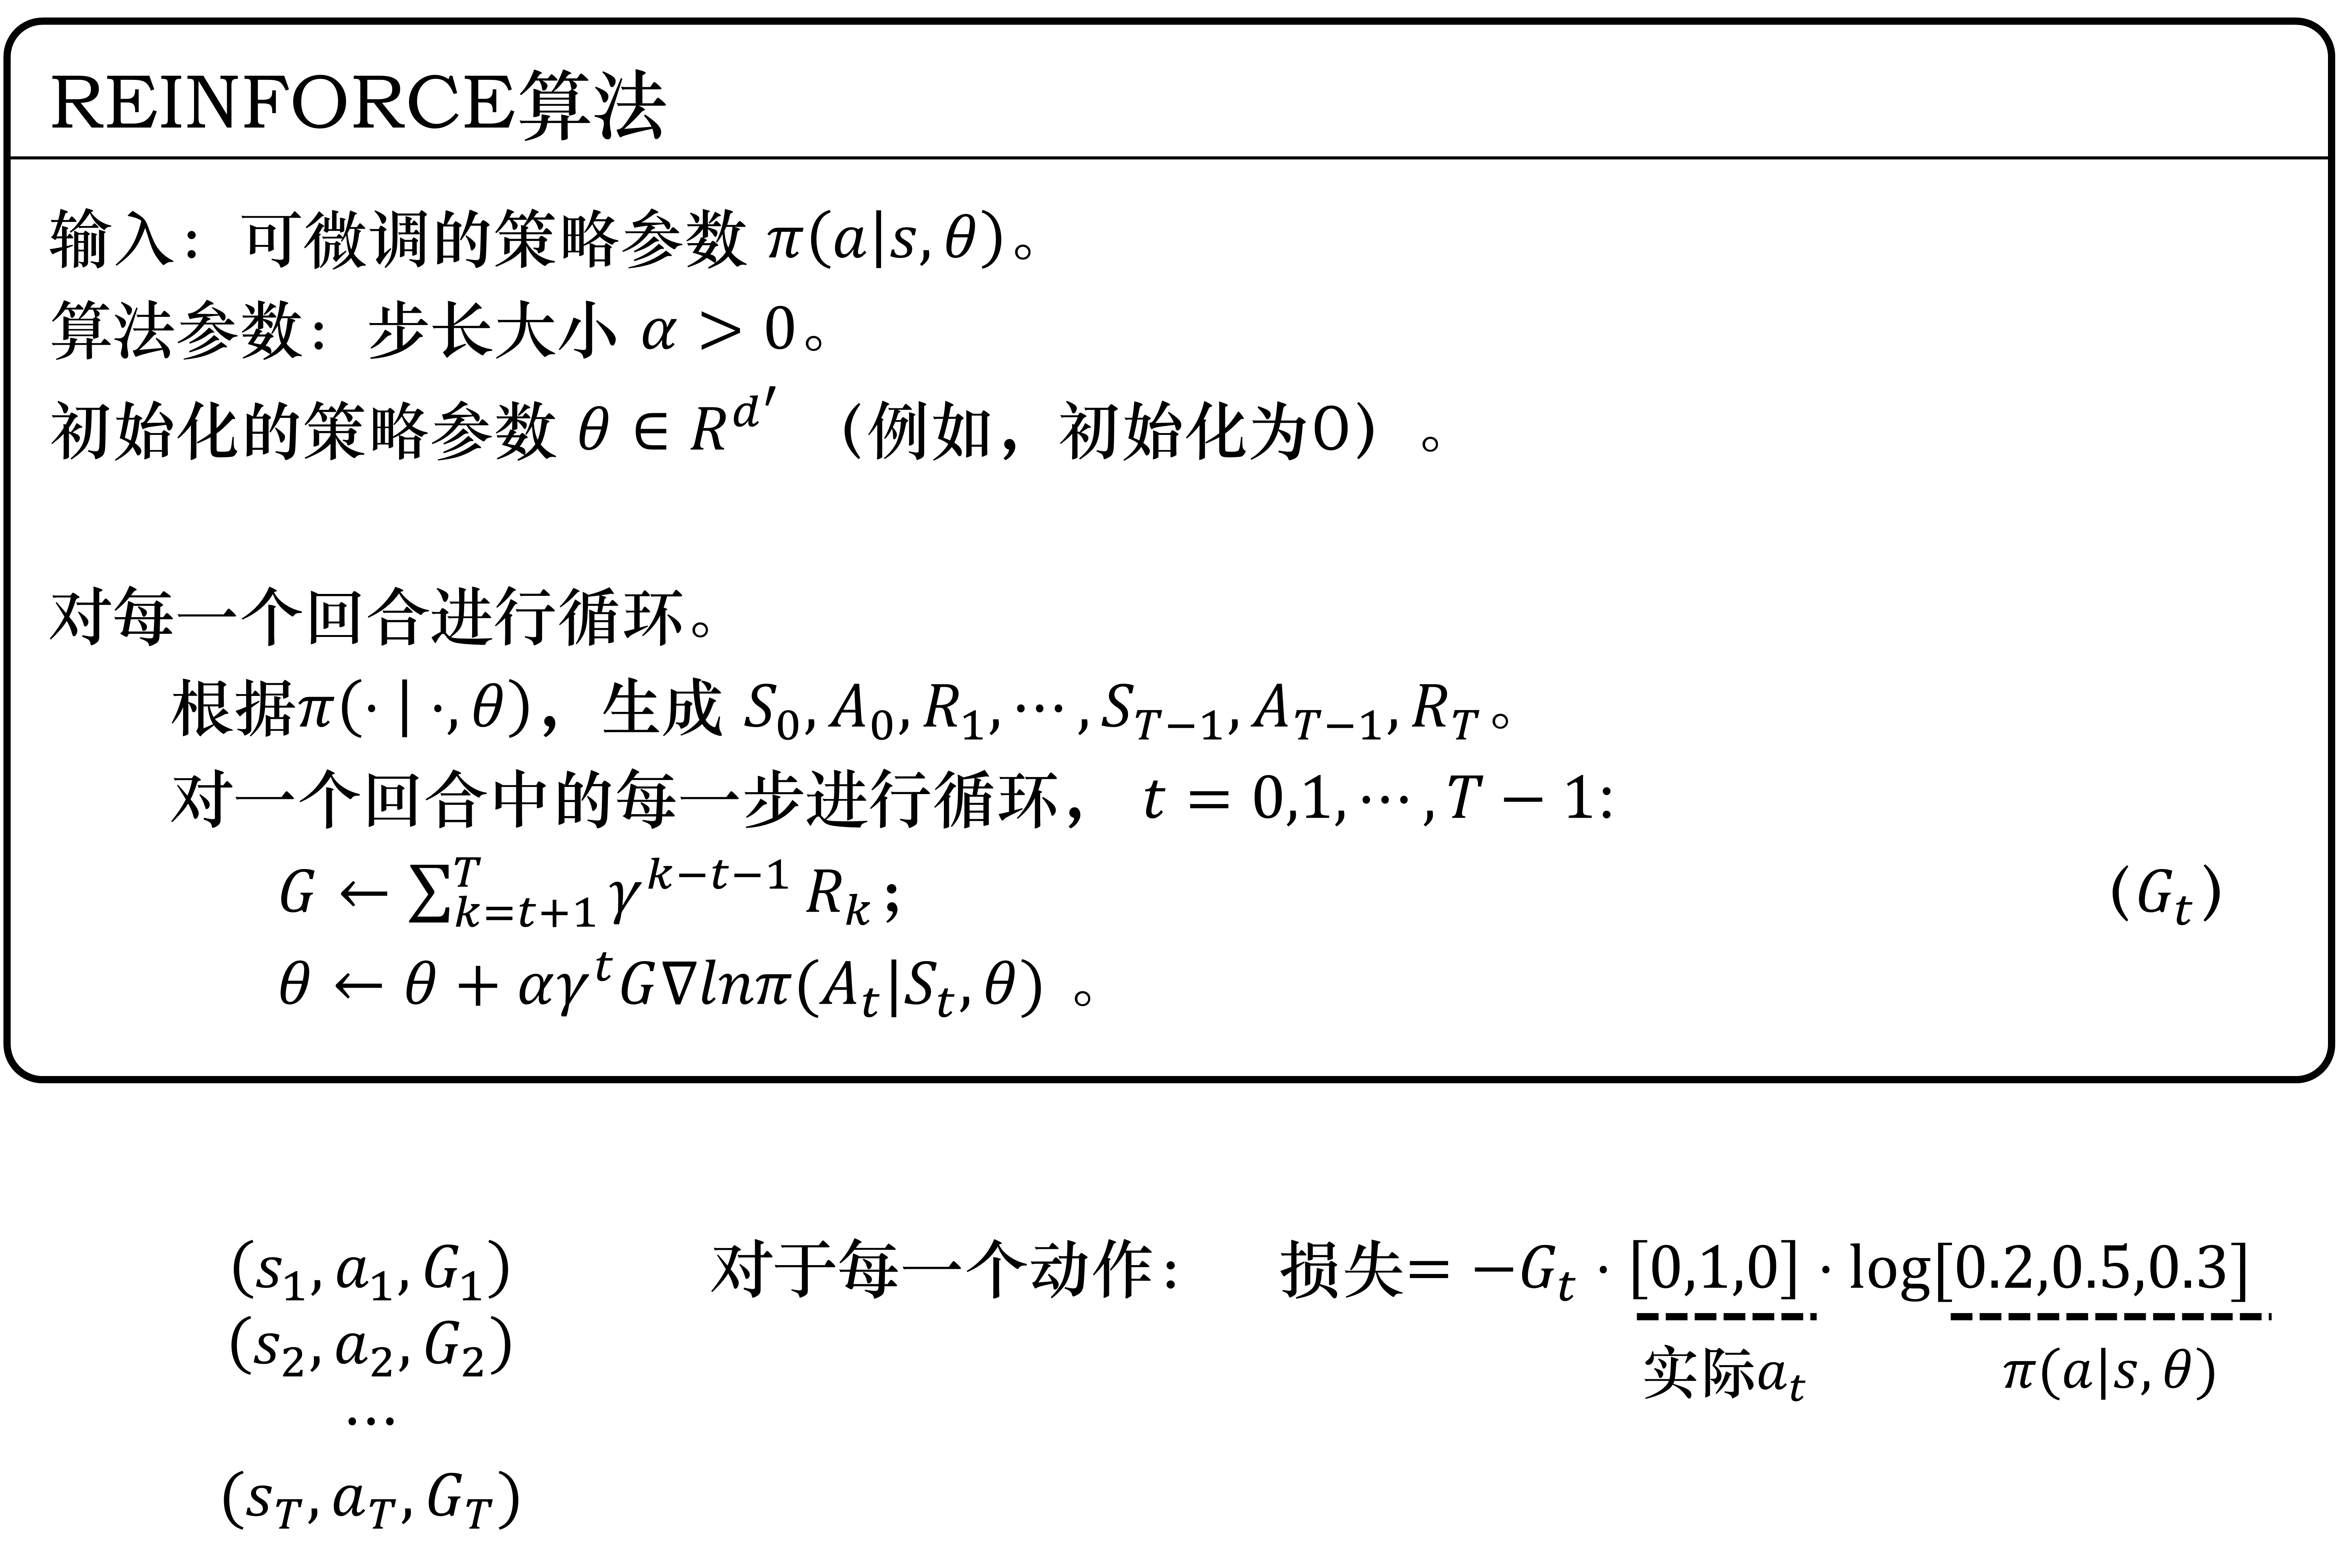
\includegraphics[width=0.5\linewidth]{ch6/figs/REINFORCE.png}
    \caption{REINFORCE算法}
    \label{fig:REINFORCE}
\end{figure}

\begin{tcolorbox}[colframe=blue!25,colback=blue!10]
独热编码(one-hot encoding)通常用于处理类别间不具有大小关系的特征。 例如血型,一共有4个取值(A型、B型、AB型、O型),独热编码会把血型变成一个4维稀疏向量,A型血表示为$[1,0,0,0]$,B型血表示为$[0,1,0,0]$,AB型血表示为$[0,0,1,0]$,O型血表示为$[0,0,0,1]$,\upcite{zhugesheng}。
\end{tcolorbox}

如\figref{fig:mnist_recognition} 所示,
手写数字识别是一个经典的多分类问题,输入是一张手写数字的图片,经过神经网络处理后,输出的是各个类别的概率。我们希望输出的概率分布尽可能地贴近真实值的概率分布。
因为真实值只有一个数字 9,所以如果我们用独热向量的形式给它编码,也可以把真实值理解为一个概率分布,9 的概率就是1,其他数字的概率就是 0。
神经网络的输出一开始可能会比较平均,通过不断地迭代、训练优化之后,我们会希望输出9 的概率可以远高于输出其他数字的概率。

\begin{figure}[hbt]
    \centering
    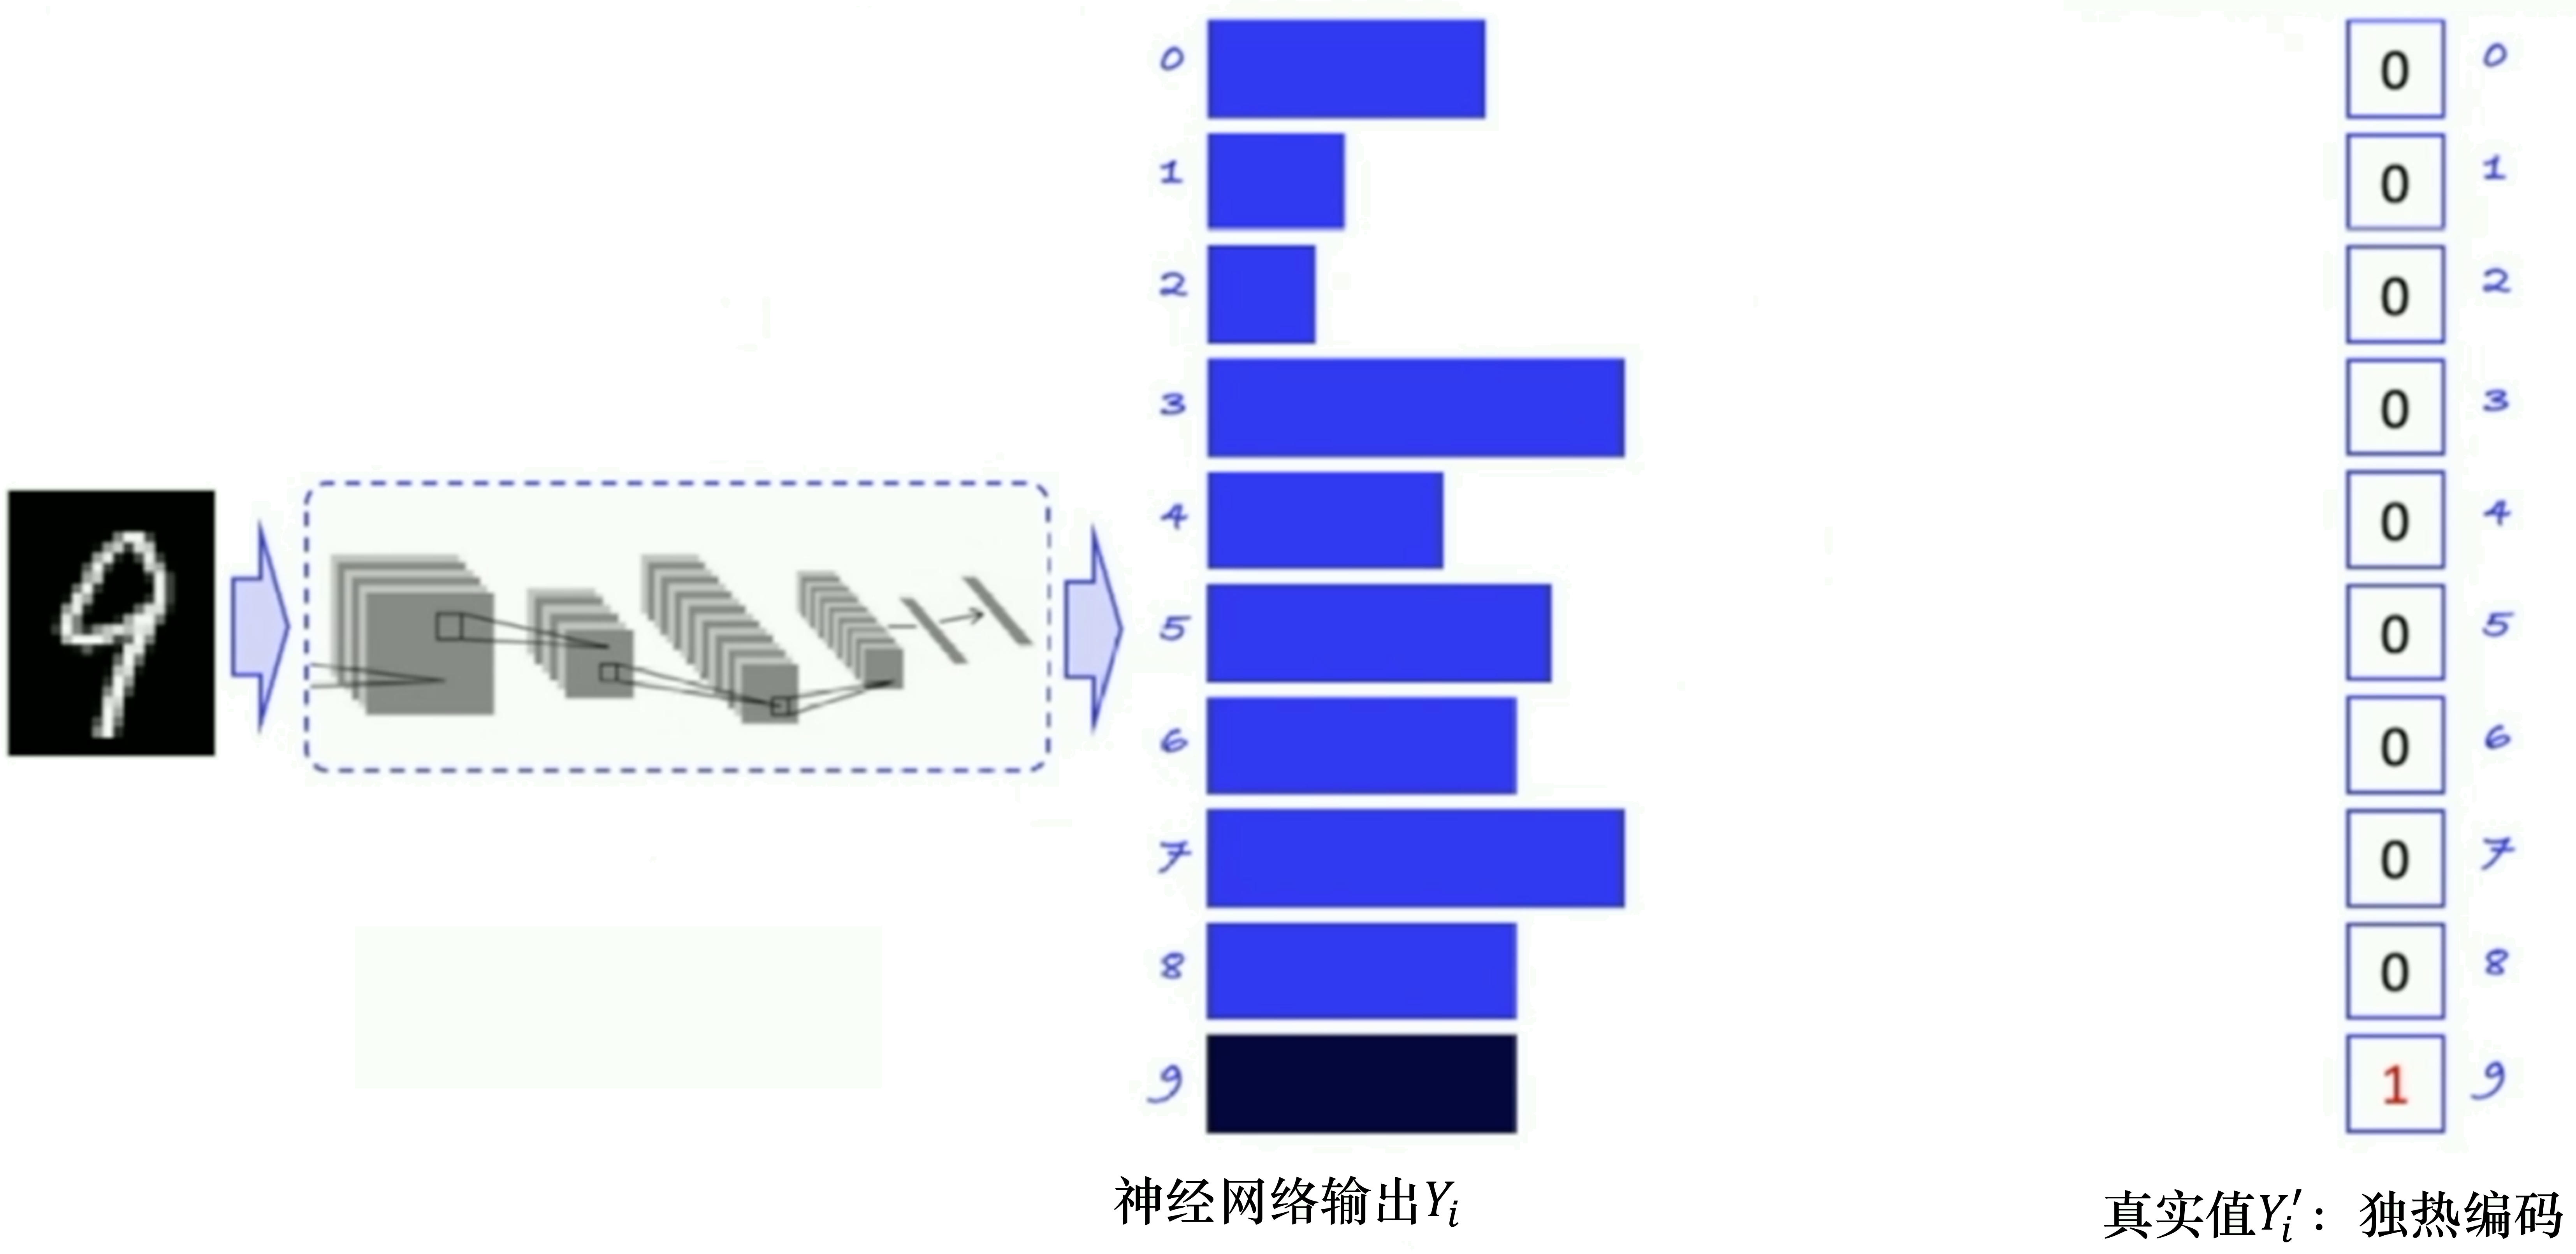
\includegraphics[width=0.5\linewidth]{ch6/figs/mnist_recognition.png}
    \caption{监督学习例子:手写数字识别}
    \label{fig:mnist_recognition}
\end{figure}

如\figref{fig:improve_nine_prob} 所示,我们所要做的就是提高输出 9 的概率,降低输出其他数字的概率,让神经网络输出的概率分布能够更贴近真实值的概率分布。我们可以用交叉熵来表示两个概率分布之间的差距。

\begin{figure}[hbt]
    \centering
    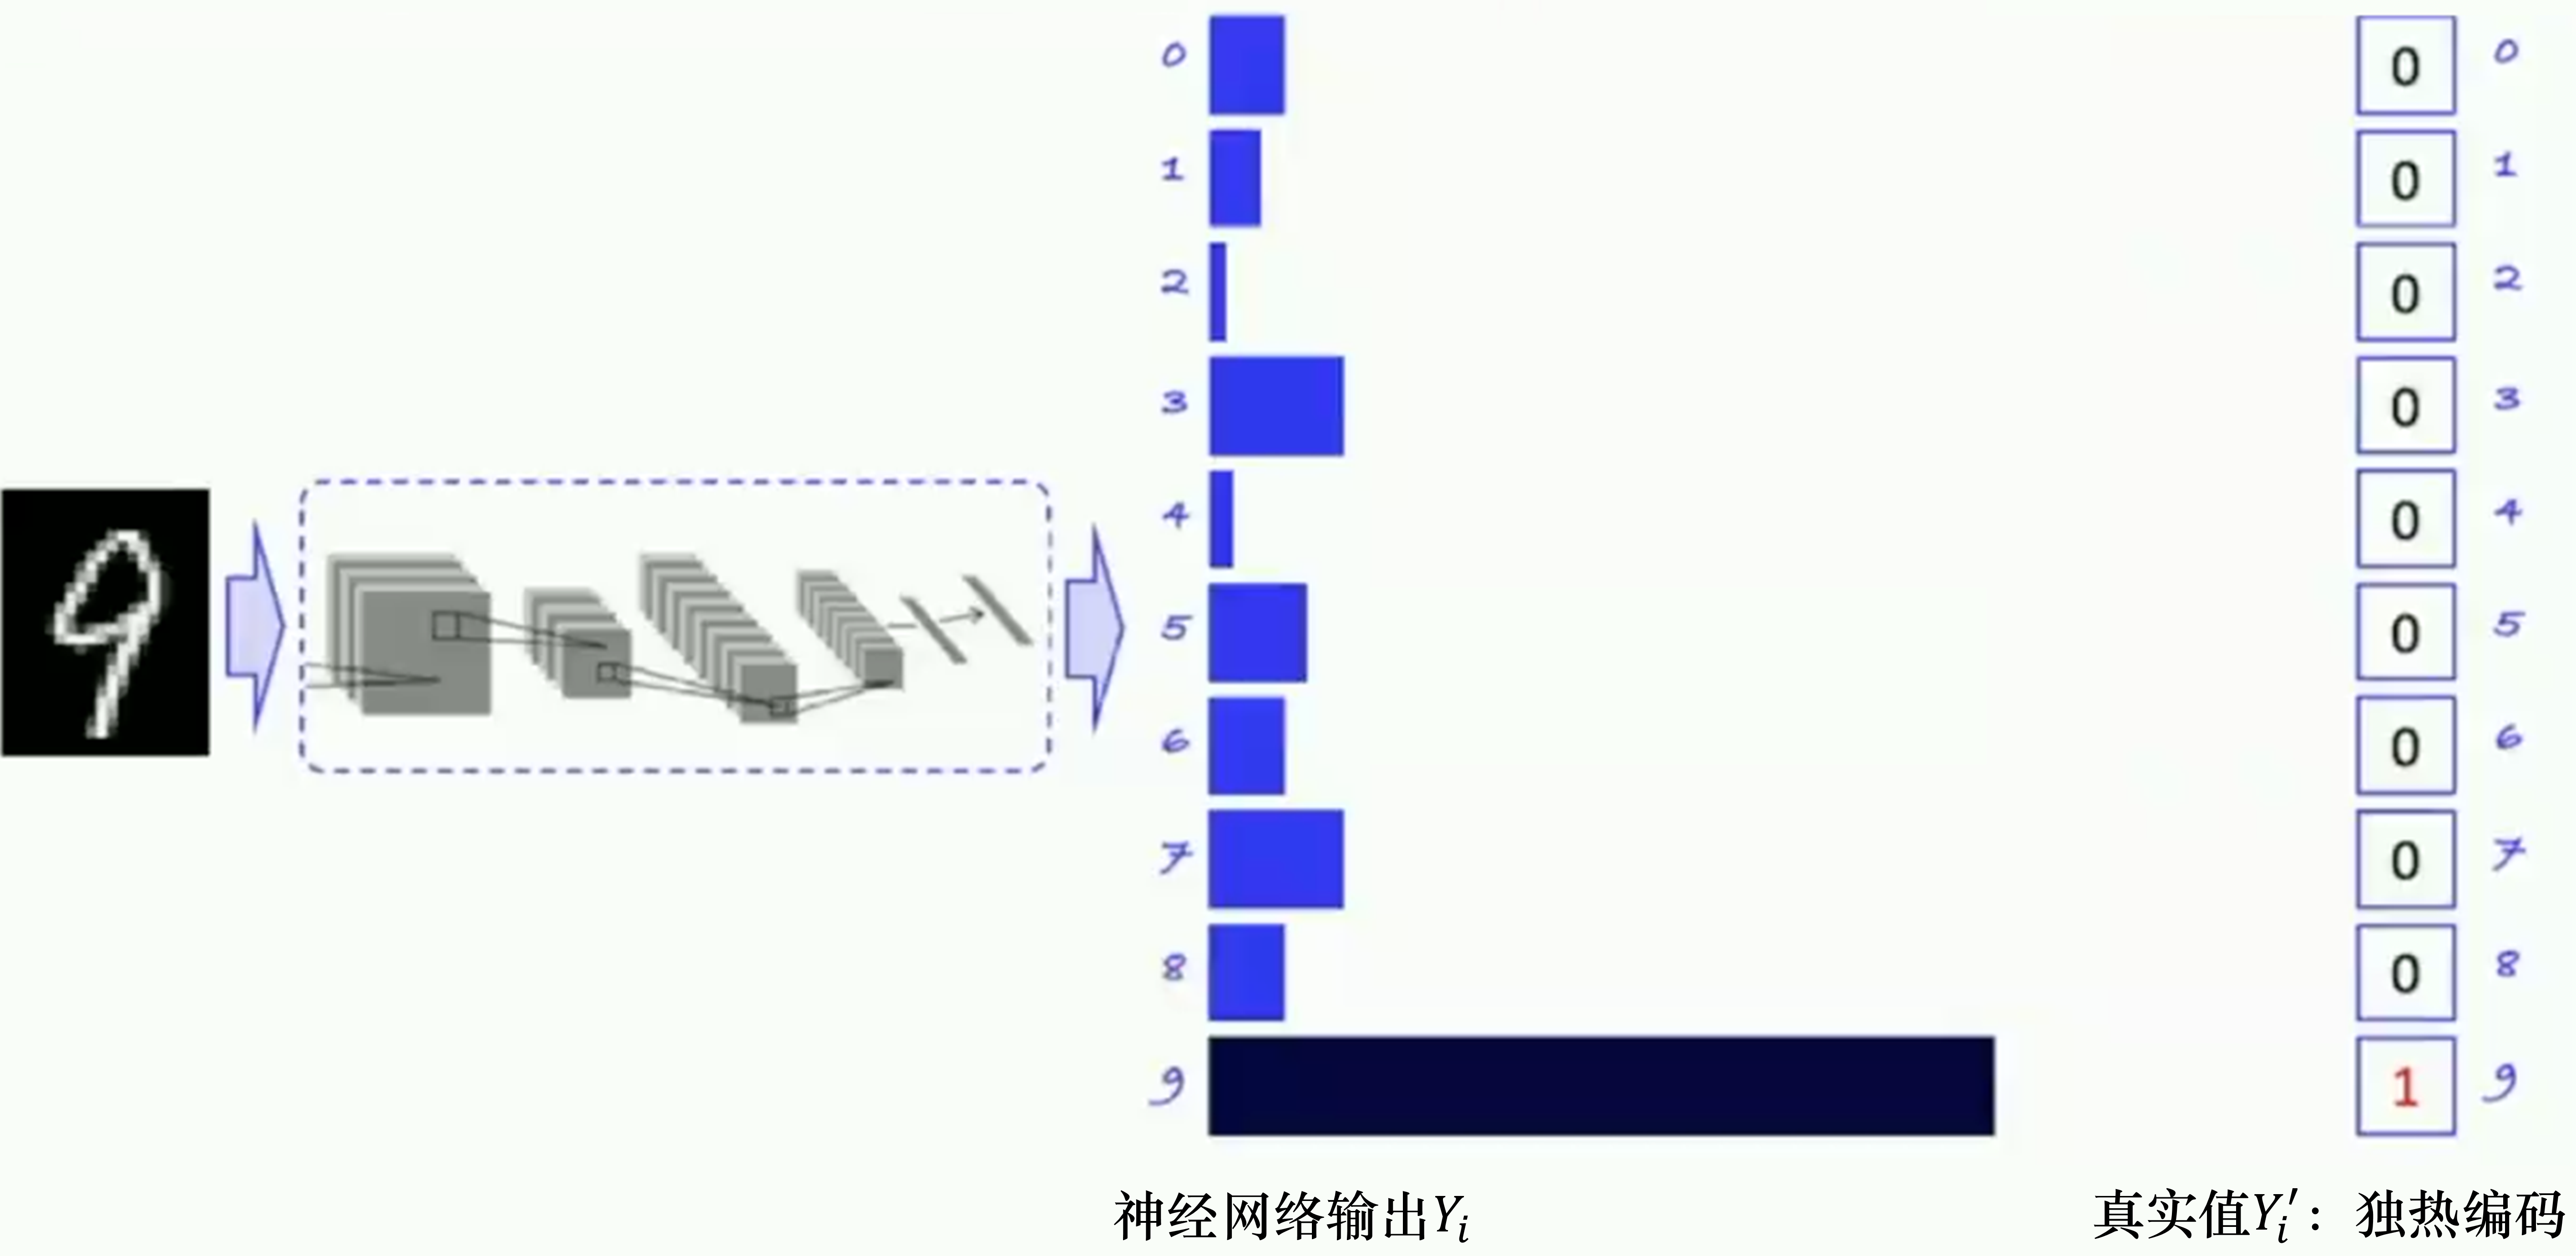
\includegraphics[width=0.5\linewidth]{ch6/figs/improve_nine_prob.png}
    \caption{提高数字9的概率}
    \label{fig:improve_nine_prob}
\end{figure}

我们看一下监督学习的优化流程,即怎么让输出逼近真实值。
如\figref{fig:opti_process} 所示,
监督学习的优化流程就是将图片作为输入传给神经网络,神经网络会判断图片中的数字属于哪一类数字,输出所有数字可能的概率,再计算交叉熵,即神经网络的输出 $Y_i$ 和真实的标签值 $Y_i'$ 之间的距离 $-\sum Y_{i}^{\prime} \cdot \log \left(Y_{i}\right)$。我们希望尽可能地缩小这两个概率分布之间的差距,计算出的交叉熵可以作为损失函数传给神经网络里面的优化器进行优化,以自动进行神经网络的参数更新。
\begin{figure}[hbt]
    \centering
    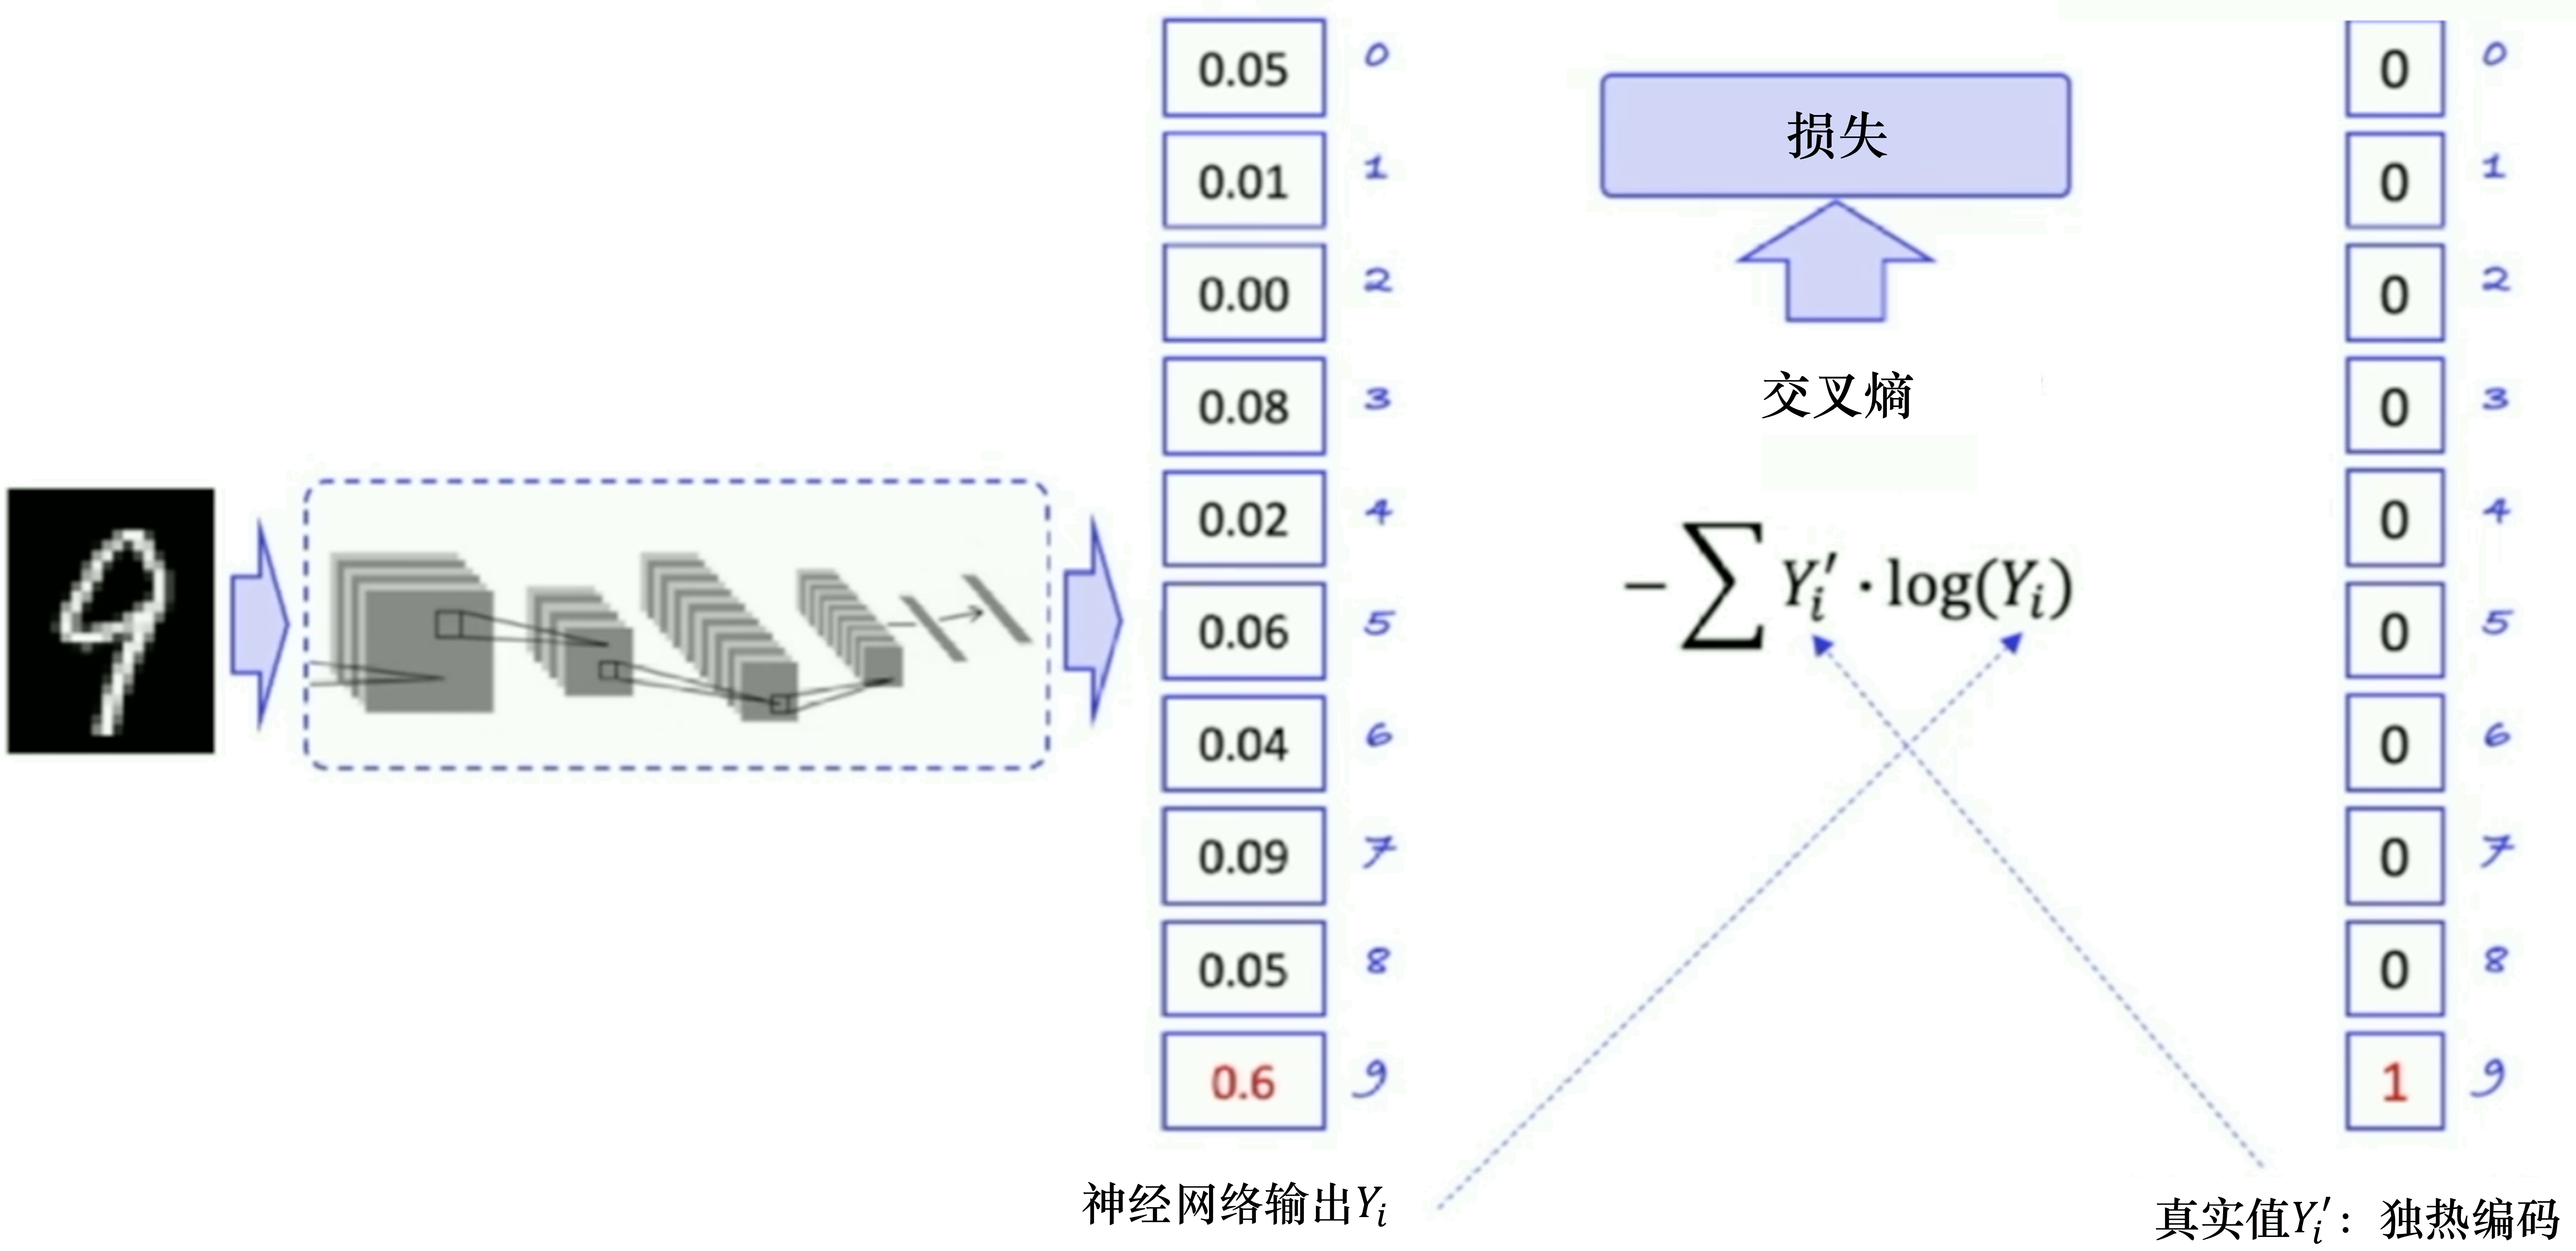
\includegraphics[width=0.5\linewidth]{ch6/figs/opti_process.png}
    \caption{优化流程}
    \label{fig:opti_process}
\end{figure}

类似地,如\figref{fig:pg_loss} 所示,策略梯度预测每一个状态下应该要输出的动作的概率,即输入状态 $s_t$,输出动作$a_t$的概率,比如 0.02、0.08、0.9。实际上输出给环境的动作是随机选择一个动作,比如我们选择向右这个动作,它的独热向量就是(0,0,1)。
我们把神经网络的输出和实际动作代入交叉熵的公式就可以求出输出动作的概率和实际动作的概率之间的差距。
但实际的动作 $a_t$ 只是我们输出的真实的动作,它不一定是正确的动作,它不能像手写数字识别一样作为一个正确的标签来指导神经网络朝着正确的方向更新,所以我们需要乘一个奖励回报 $G_t$。$G_t$相当于对真实动作的评价。
如果 $G_t$ 越大,未来总奖励越大,那就说明当前输出的真实的动作就越好,损失就越需要重视。
如果 $G_t$ 越小,那就说明动作 $a_t$ 不是很好,损失的权重就要小一点儿,优化力度也要小一点儿。
通过与手写数字识别的一个对比,我们就知道为什么策略梯度损失会构造成这样。
\begin{figure}[hbt]
    \centering
    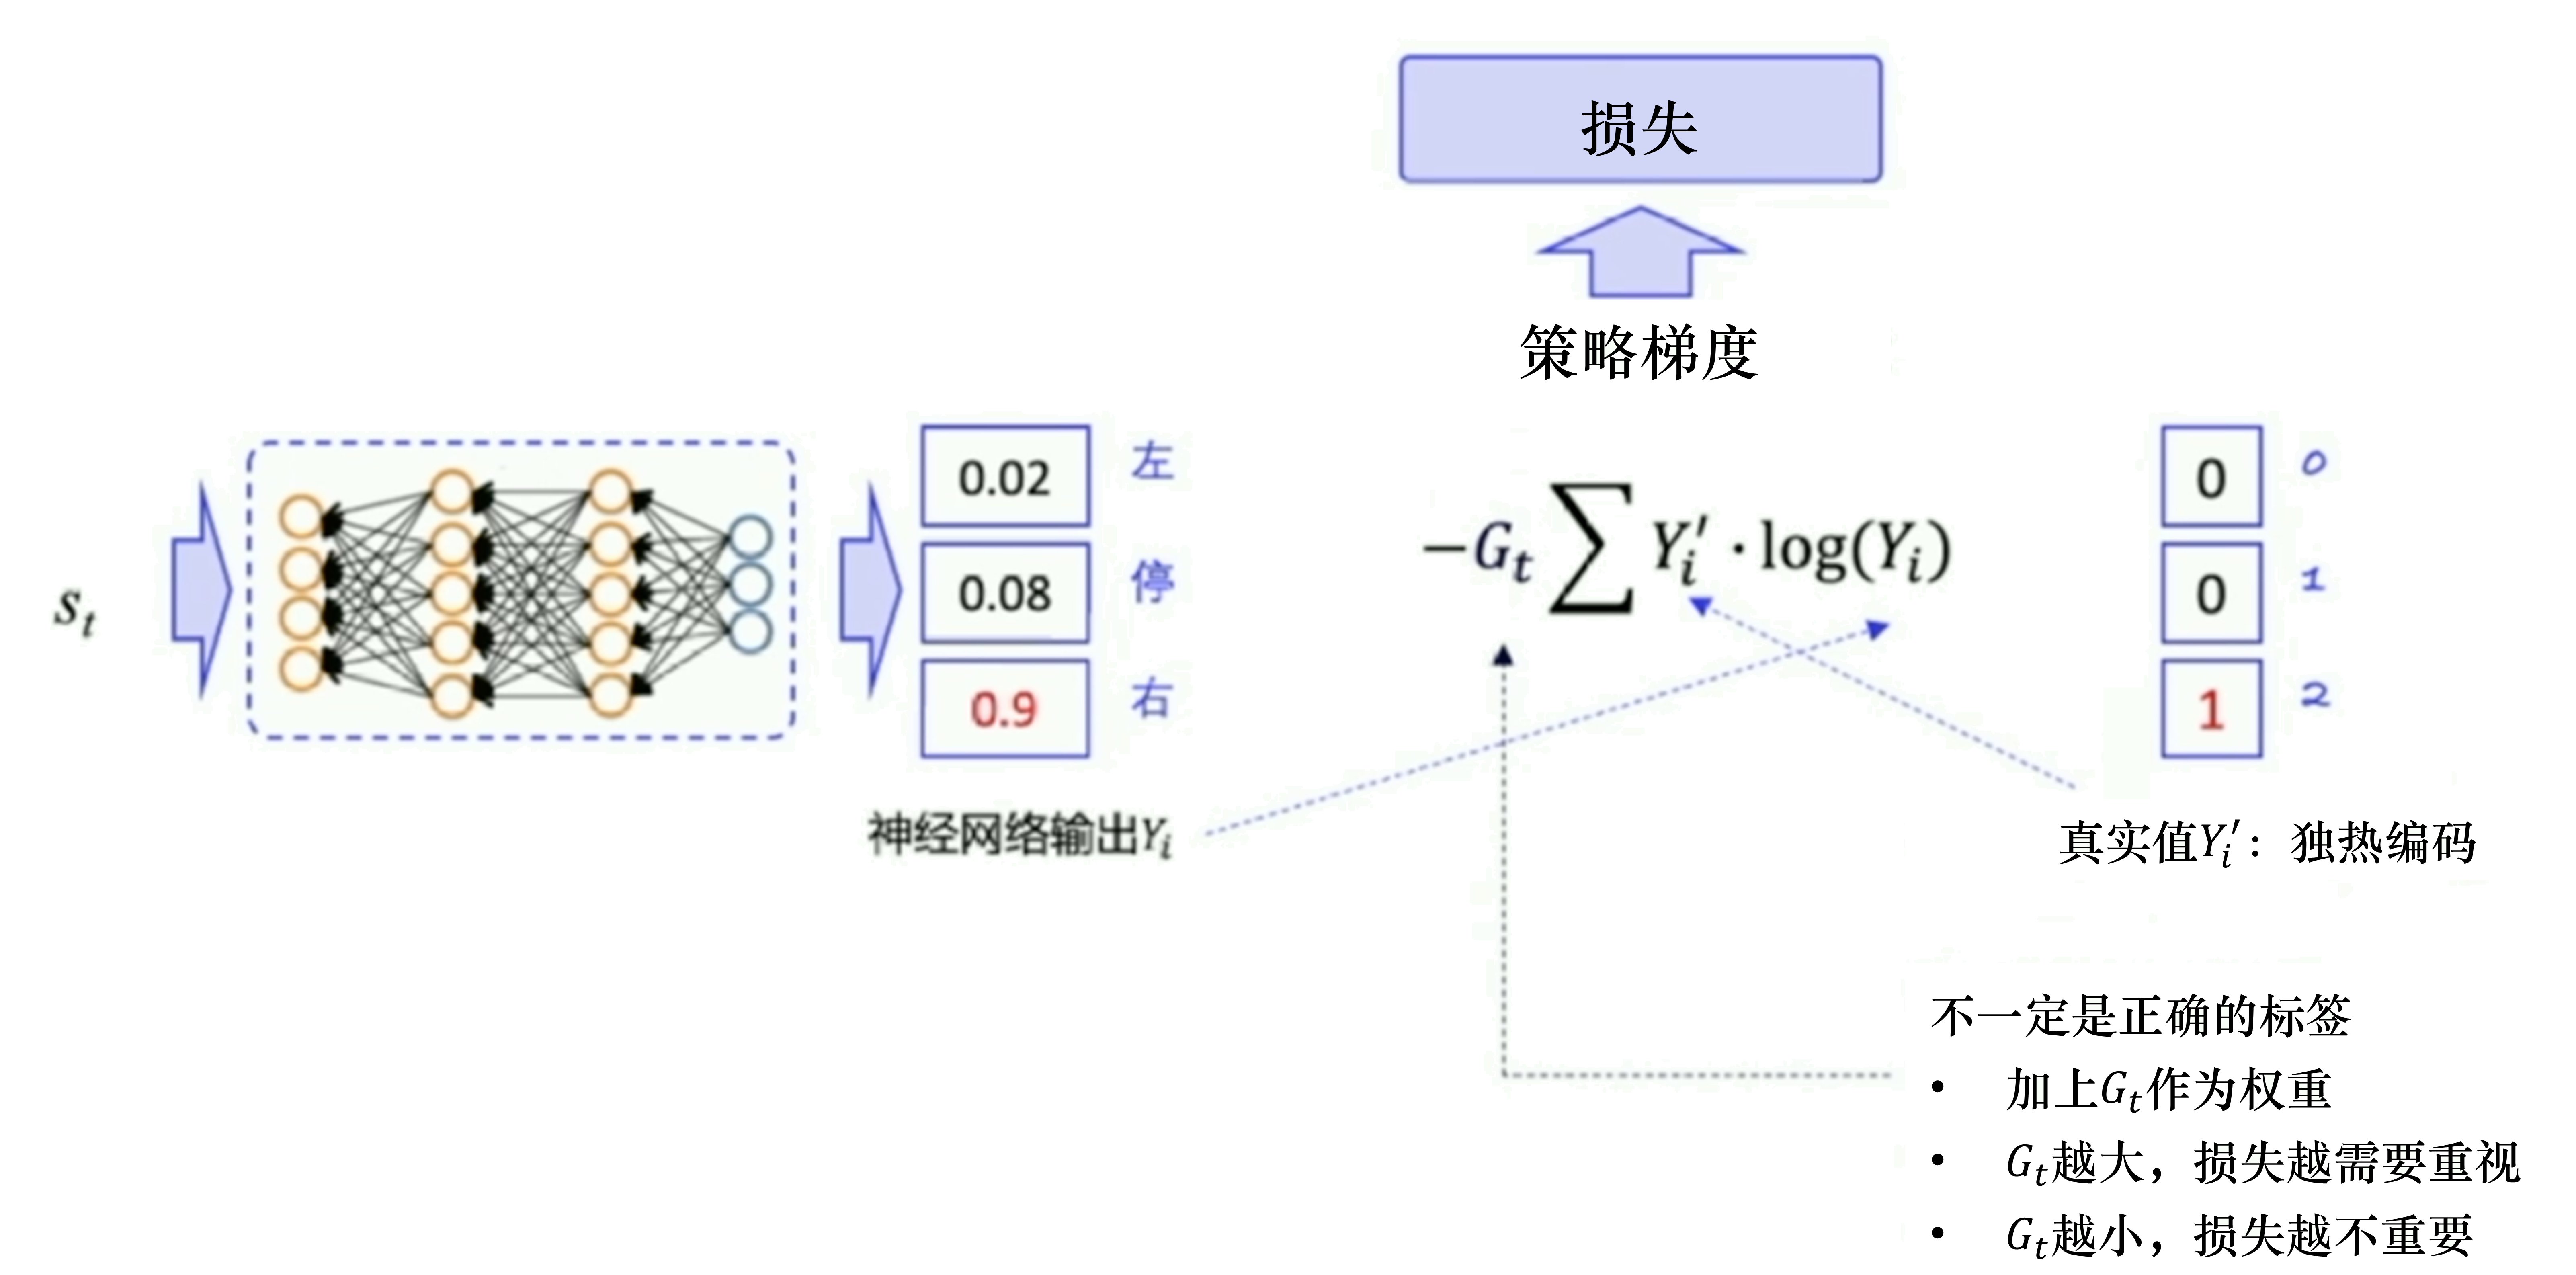
\includegraphics[width=0.5\linewidth]{ch6/figs/pg_loss.png}
    \caption{策略梯度损失}
    \label{fig:pg_loss}
\end{figure}

如\figref{fig:loss_compute} 所示,
实际上我们在计算策略梯度损失的时候,要先对实际执行的动作取独热向量,
% 拿到那个 $\ln \pi(a_t|s_t,\theta)$。我就拿实际执行的这个动作,
再获取神经网络预测的动作概率,将它们相乘,我们就可以得到 $\ln \pi(a_t|s_t,\theta)$,这就是我们要构造的损失。
因为我们可以获取整个回合的所有的轨迹,所以我们可以对这一条轨迹里面的每个动作都去计算一个损失。把所有的损失加起来,我们再将其“扔”给 Adam 的优化器去自动更新参数就好了。
\begin{figure}[hbt]
    \centering
    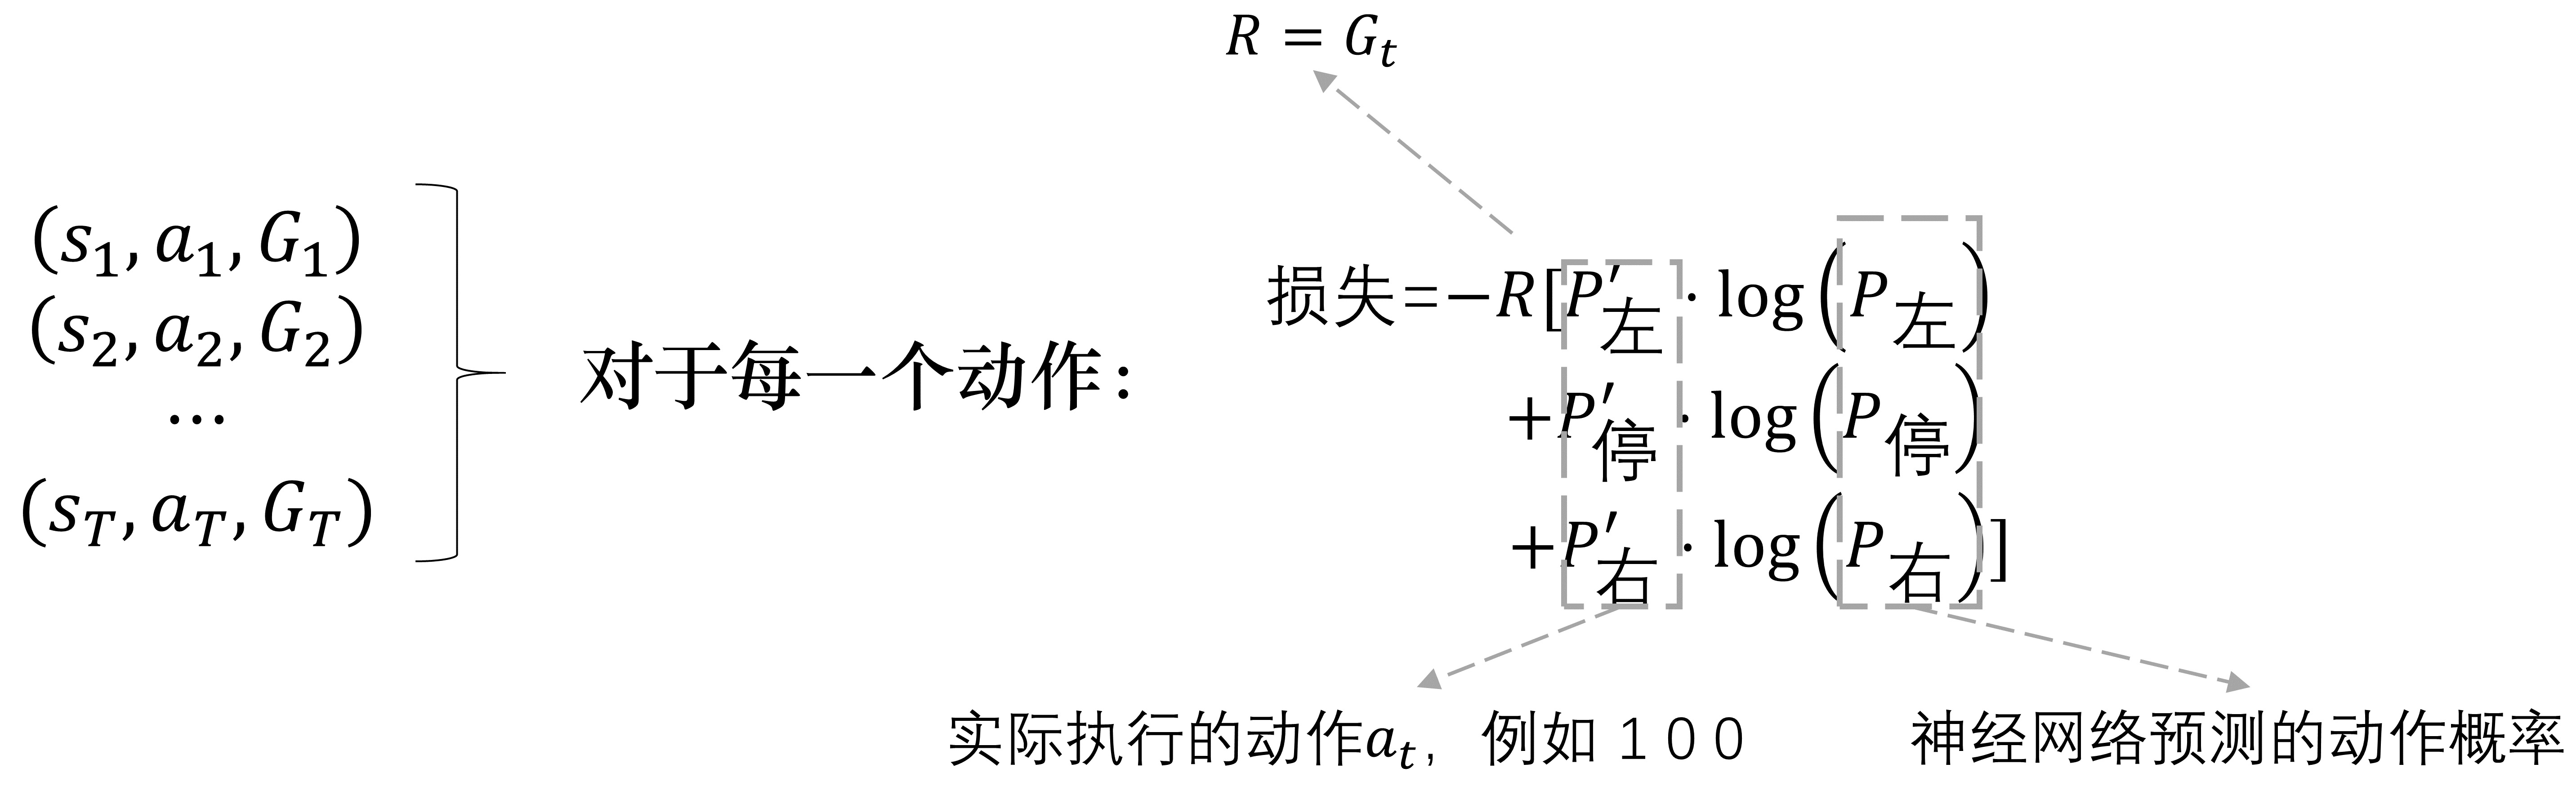
\includegraphics[width=0.5\linewidth]{ch6/figs/loss_compute.png}
    \caption{损失计算}
    \label{fig:loss_compute}
\end{figure}

\figref{fig:REINFORCE_process} 所示为 REINFORCE 算法示意图,首先我们需要一个策略模型来输出动作概率,输出动作概率后,
通过 \kw{sample()} 函数得到一个具体的动作,与环境交互后,我们可以得到整个回合的数据。得到回合数据之后,我们再去执行\kw{learn()} 函数,在 \kw{learn()} 函数里面,我们就可以用这些数据去构造损失函数,“扔”给优化器优化,更新我们的策略模型。
\begin{figure}[hbt]
    \centering
    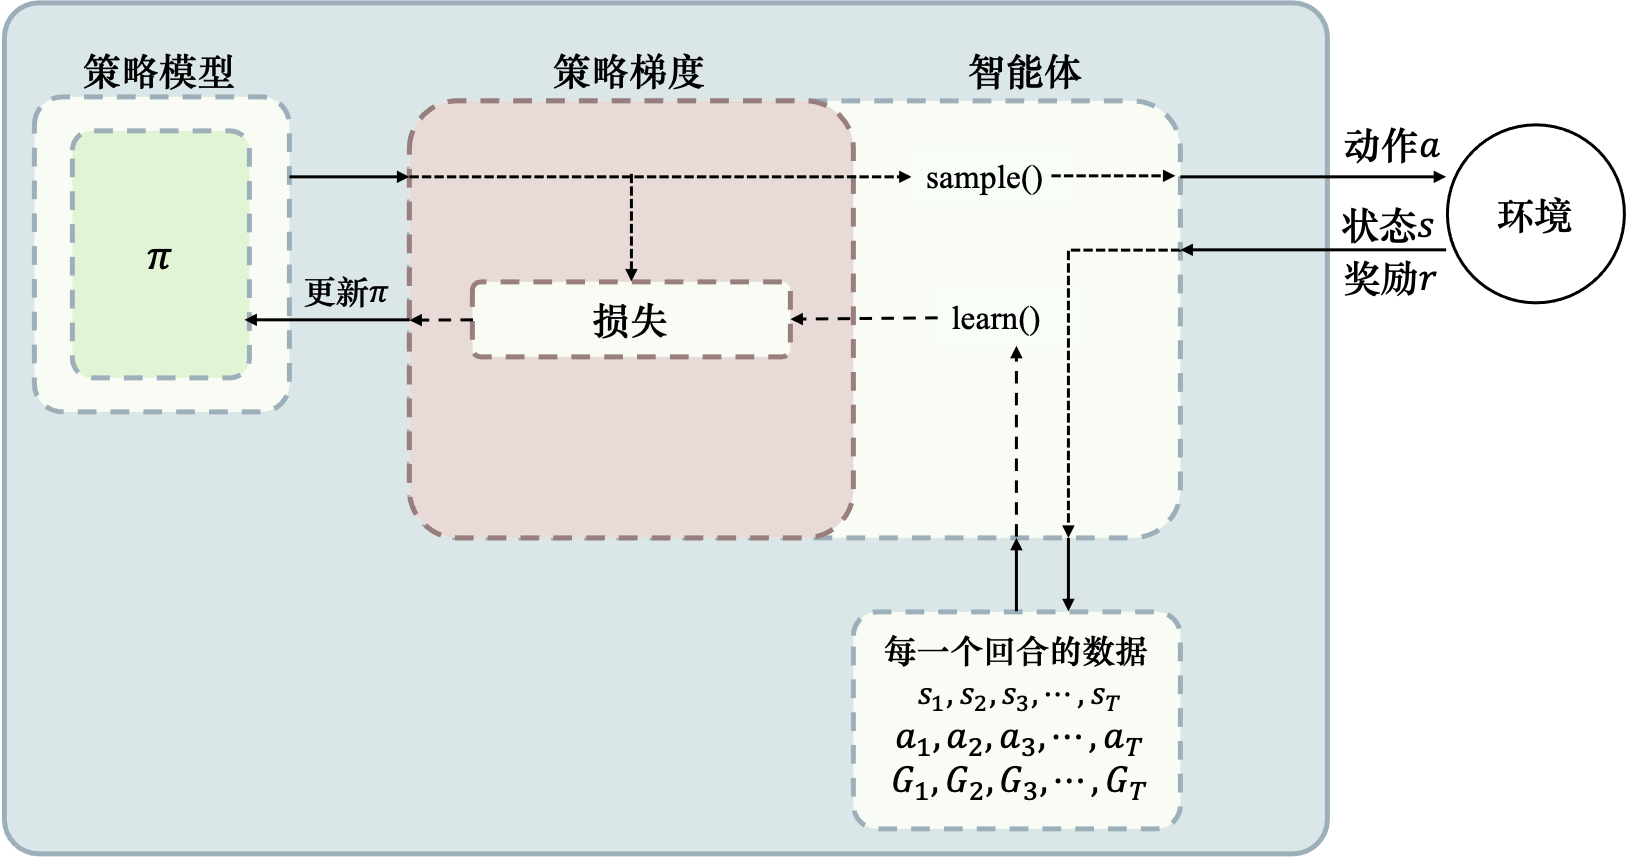
\includegraphics[width=0.5\linewidth]{ch6/figs/REINFORCE_process.png}
    \caption{REINFORCE算法示意}
    \label{fig:REINFORCE_process}
\end{figure}

\subsection{策略梯度的进阶推导}

在上一节中我们通过计算轨迹的概率并乘上对应的价值,然后将通过全期望公式将这些项累加起来就得到了关于策略的总价值期望,即我们要求得的目标函数,如\eqref{eq:expect_policy_2}所示。
\begin{equation}
    \label{eq:expect_policy_2}
    \begin{aligned}
    J(\pi_{\theta}) = P_{\theta}(\tau_{1})R(\tau_{1})+P_{\theta}(\tau_{2})R(\tau_{2})+\cdots \\
    &=\int_\tau P_{\theta}(\tau) R(\tau) \\ 
\end{aligned}
\end{equation}
然后通过对数微分等技巧求出对应的梯度,如\eqref{eq:pg_ob_grad_2}所示。
\begin{equation}
    \label{eq:pg_ob_grad_2}
    \begin{aligned}
    \nabla_\theta J\left(\pi_\theta\right) = \underset{\tau \sim \pi_\theta}{\mathrm{E}}\left[\sum_{t=0}^T \nabla_\theta \log \pi_\theta\left(a_t \mid s_t\right) R(\tau)\right]
    \end{aligned}
\end{equation}

那么问题来了,可以看到无论是目标函数还是对应的梯度都必须求出关于轨迹$\tau$的项,例如$R(\tau)$。乍一看这个包含轨迹的项似乎比较容易求,但实际上是很难的,就像我们某些玩家日常指挥别人打游戏时那样,嘴上说说容易,实际操作起来却发现处处是细节。为什么说处处是细节呢?注意看\eqref{eq:pg_ob_grad_2}中对于$\log \pi_\theta\left(a_t \mid s_t\right)$中的每一个状态-动作对$(s_t,a_t)$,我们都需要求出对应的累积奖励$R(\tau)$。我们当然可以先把每一条从初始状态$s_0$到当前状态$s_t$所经历的轨迹对应的每一步奖励存储起来然后求出最终的累积奖励$R(\tau)$,即便 REINFORCE 算法在计算轨迹对应的价值方面做了一定的优化,但一个状态$s_t$背后的累积价值和梯度是需要通过包含很多个历史状态的轨迹来计算的,光是这样想恐怕读者们眼泪都要止不住掉下来。其次我们观察\eqref{eq:expect_policy_2},我们是要将所有轨迹的概率和对应的累积奖励相乘然后累加得到最终的价值期望,也就是目标函数。那么这里所有的轨迹是哪些轨迹呢?怎么数出来的?可能有些读者会说我们可以先搜集一些轨迹来近似所有轨迹,那么到底要搜集多少条轨迹才能近似?当然你可以搜集成千上万条,但恐怕还没等你计算完这些轨迹的期望其他人可能都已经用 DQN 算法完美解决这个问题了。我们原本认为直接通过对策略的梯度进行优化会比以间接的方式先估计对应的价值然后选择动作收敛的速度要更快,如果计算轨迹期望都这么麻烦似乎失去了实现策略梯度算法的初衷。并且还有一个很重要的问题,如\figref{fig:traj_compute}所示(补一张类似于条条大路通罗马的可爱动漫图),实际过程中初始状态$s_0$到当前状态$s_t$的轨迹应该不止一条,我可能走一步就到了状态$s_t$,也可能走了很多步才到$s_t$,走一步和走很多步生成的轨迹对应的累积奖励多数情况下也是不一样的,这个时候我们是多个轨迹都算进去还是只考虑其中一条呢?

\begin{figure}[hbt]
    \centering
    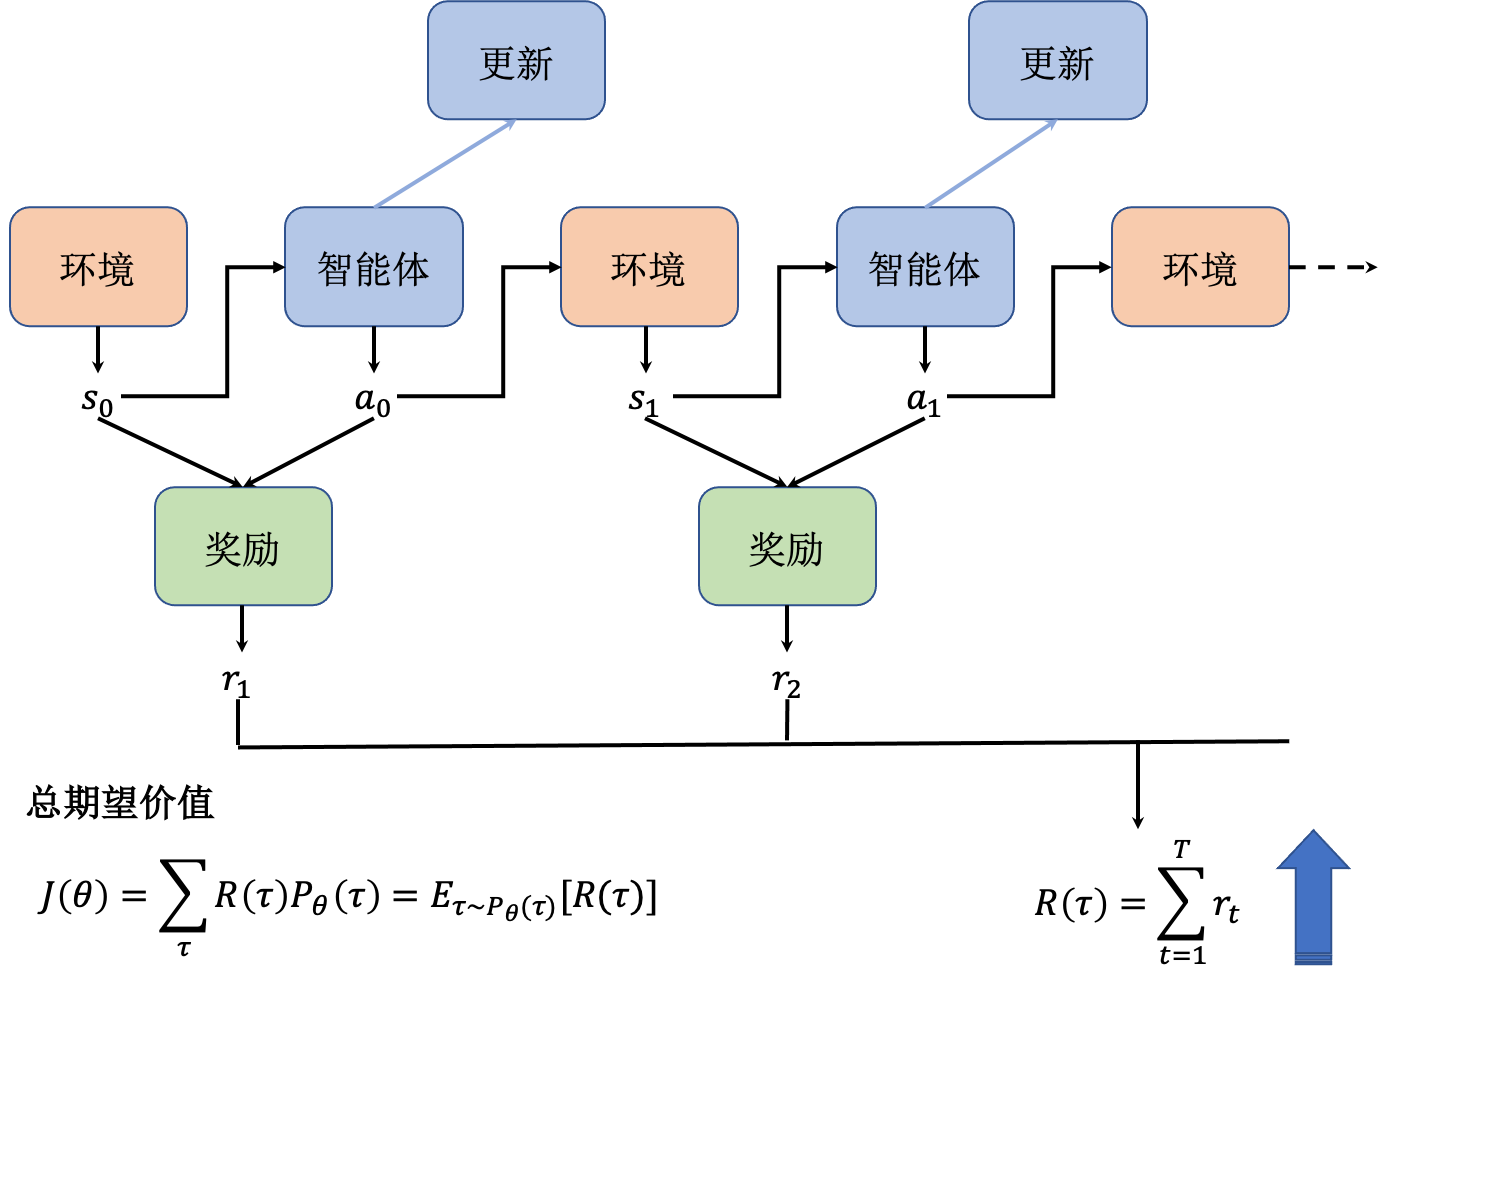
\includegraphics[width=0.5\linewidth]{ch6/figs/expected_reward.png}
    \caption{轨迹的计算}
    \label{fig:traj_compute}
\end{figure}

这样绕来绕去始终得不到一个准确的答案,这个时候可能就会有读者灵光乍现,我们在马尔科夫决策过程中计算的奖励不应该是“长期奖励”吗?那么这时候恭喜你没有被调皮的作者绕进去!实际上,在所有的马尔可夫过程中我们优化的目标都是“长期”的价值期望,不明白的读者可以再温习一下马尔可夫决策过程的定义以及前面Q learning算法相关的推导内容,相信你一定能够回顾起来所谓“长期”的意义。暂时给一个小的结论,我们这里选择的轨迹和对应的累积价值都应该是长期的轨迹和价值,如此才能保证我们的目标函数计算出来的也是长期的总价值。换句话说,对于每条轨迹,从初始状态$s_0$到当前状态$s_t$所经历的步数应该是无限的,即$t \rightarrow \infty$。这时候读者可能会奇怪,有限步数就已经够难算了,无限步数还能算出来吗?答案是可以的,而且更简便快捷,在数学中就是这样,“无限的”往往比“有限的”更容易计算出来,这里就涉及到一个重要的概念,即马尔可夫链的平稳分布,还请跟随笔者的思路到下一小节详细了解什么是马尔可夫链的平稳分布。

\subsubsection{平稳分布}

在本小节中我们将会详细了解什么是马尔可夫链的平稳分布,先不急着抛出一堆抽象的概念和公式,我们先来看一个经典的例子。这个例子是这样的,社会学家在他们的研究中通常会把人按照经济状况分成三类:上层,中层和下层,这三层就代表着三种状态,我们分别用 1,2,3 来表示。并且社会学家还发现决定一个人经济阶层的最重要因素就是其父母的收入阶层,即如果一个人的经济阶层为上层,那么他的孩子会有 0.5 的概率继续处于上层,也会有 0.4 的概率变成中层,更有 0.1 的概率降到下层,当然这些概率数值只是笔者拍脑袋想出来以便于后面的计算的,并没有一定的统计依据。这些概率其实就是我们所说的马尔可夫链中的转移概率,同样对于其他经济阶层的人他们的孩子也会有一定的概率变成上、中、下的任一经济阶层,如\figref{fig:markov_economy}所示。

\begin{figure}[hbt]
    \centering
    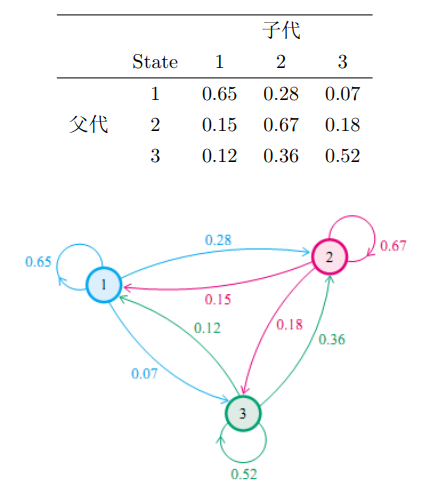
\includegraphics[width=0.5\linewidth]{ch6/figs/markov_economy.png}
    \caption{期望的奖励}
    \label{fig:markov_economy}
\end{figure}

这样我们就可以列出转移概率矩阵,如\eqref{eq:tran_prob_economy}所示。

\begin{equation}
    \label{eq:tran_prob_economy}
    P=\left[\begin{array}{lll}
    0.5 & 0.4 & 0.1 \\
    0.2 & 0.6 & 0.2 \\
    0.05 & 0.45 & 0.5
    \end{array}\right]
\end{equation}

我们假设有这么一批数量足够的人,称之为第 1 代人,他们的经济阶层比例为$\pi_0=[0.15,0.62,0.23]$,那么根据上面的转移概率矩阵我们就可以求出第二代的阶层比例。怎么求呢?首先求出第二代上层的比例,我们知道第一代人中有 0.15 的比例是上层,这 0.15 比例的人中子代为上层的概率是 0.5, 而第一代人中 0.62 比例的中层会有 0.2 的概率流入上层,0.23 比例的下层中其子代也会有 0.05 的概率流入上层,那么最后第二代上层的比例就为 $0.15 \times 0.5 + 0.62 \times 0.2 + 0.23 \times 0.05 = 0.2105 \approx 0.210$,依次类推,第二代中层的比例为$0.15 \times 0.4 + 0.62 \times 0.6 + 0.23 \times 0.45 \approx 0.536$,第二代下层的比例为$0.254$,这样我们就能得出第二代的阶层比例为$\pi_1=[0.210,0.536,0.254]$。这里细心的读者会发现不需要这么麻烦的计算过程,只要学过线性代数利用矩阵向量相乘就能得到,即$\pi_1 = \pi_0 P = [0.210,0.536,0.254]$。同理,第二代人的比例也可以求出,即 $\pi_2 = \pi_1 P = \pi_0 P^2$,依次类推,第n代人的比例为$\pi_n = \pi_0 P^n$。既然这本书同时也是教大家如何代码实战的,这里我们 Python 代码来求出前 10 代人的比例,如下。


\begin{lstlisting}[language=Python]
import numpy as np
pi_0 = np.array([[0.15,0.62,0.23]])
P = np.array([[0.5,0.4,0.1],[0.2,0.6,0.2],[0.05,0.45,0.5]])
for i in range(1,10+1):
    pi_0 = pi_0.dot(P)
    print(f"第{i}代人的比例为:")
    print(np.around(pi_0,3))
\end{lstlisting}

我们可以很快获得计算的结果,如下。

\begin{lstlisting}[language=Bash]
第1代人的比例为:
[[0.211 0.536 0.254]]
第2代人的比例为:
[[0.225 0.52  0.255]]
第3代人的比例为:
[[0.229 0.517 0.254]]
第4代人的比例为:
[[0.231 0.516 0.253]]
第5代人的比例为:
[[0.231 0.516 0.253]]
第6代人的比例为:
[[0.231 0.516 0.253]]
第7代人的比例为:
[[0.232 0.516 0.253]]
第8代人的比例为:
[[0.232 0.516 0.253]]
第9代人的比例为:
[[0.232 0.516 0.253]]
第10代人的比例为:
[[0.232 0.516 0.253]]
\end{lstlisting}

这里忽略程序算出来的小数取舍问题,比如第一代人我们手算的比例而$[0.210,0.536,0.254]$,而程序却是$[0.211,0.536,0.254]$,这是因为程序内置保留有效数字的规则问题,不影响整体结果。回归正题,从上面的结果中,我们发现从第5代开始经济阶层的比例开始神奇地固定了下来。换句话说,无论初始状态是什么,经过多次概率转移之后都会存在一个稳定的状态分布。其次我们只需要知道这个稳定的分布并乘以对应的价值,就可以计算所谓的长期收益了。

现在我们可以正式地总结一下马尔可夫链的平稳分布了,对于任意马尔可夫链,如果满足以下两个条件:

\begin{itemize}
    \item 非周期性:由于马尔可夫链需要收敛,那么就一定不能是周期性的,实际上我们处理的问题基本上都是非周期性的,这点不需要做过多的考虑。
    \item 状态连通性:即存在概率转移矩阵$P$,能够使得任意状态$s_0$经过有限次转移到达状态$s$,反之亦然。
\end{itemize}

这样我们就可以得出结论,即该马氏链一定存在一个平稳分布,我们用$d^{\pi}(s)$表示,可得到\eqref{eq:markov_station}:

\begin{equation}
    \label{eq:markov_station}
    d^\pi(s)=\lim _{t \rightarrow \infty} P\left(s_t=s \mid s_0, \pi_\theta\right)
\end{equation}

我们回顾前面小节中计算轨迹概率的公式$P_{\theta}(\tau)$,可以发现如果轨迹$\tau$的初始状态是$s_0$并且终止状态是$s$的话,轨迹概率公式$P_{\theta}(\tau)$跟平稳分布的$d^\pi(s)$是等效的,当然前提是该条轨迹必须“无限长”,即$t \rightarrow \infty$。但是平稳分布与轨迹概率公式相比,它的好处就是只涉及一个定量即初始状态$s_0$和一个变量$s$。对于每个状态$s$,我们用$V^{\pi}(s)$表示策略$\pi$下对应的价值,读者们现在可以往前回顾,为什么笔者说策略梯度算法跟基于价值函数的算法都是在计算累积状态的价值期望了,此时策略梯度算法目标函数就可以表示为\eqref{eq:pg_station_object}。

\begin{equation}
    \label{eq:pg_station_object}
    J(\theta)=\sum_{s \in \mathcal{S}} d^\pi(s) V^\pi(s)=\sum_{s \in \mathcal{S}} d^\pi(s) \sum_{a \in \mathcal{A}} \pi_\theta(a \mid s) Q^\pi(s, a)
\end{equation}

同样可以利用对数微分技巧求得对应的梯度,如\eqref{eq:pg_station_object_grad}。

\begin{equation}
    \label{eq:pg_station_object_grad}
    \begin{aligned}
    \nabla_\theta J(\theta) & \propto \sum_{s \in \mathcal{S}} d^\pi(s) \sum_{a \in \mathcal{A}} Q^\pi(s, a) \nabla_\theta \pi_\theta(a \mid s) \\
    &=\sum_{s \in \mathcal{S}} d^\pi(s) \sum_{a \in \mathcal{A}} \pi_\theta(a \mid s) Q^\pi(s, a) \frac{\nabla_\theta \pi_\theta(a \mid s)}{\pi_\theta(a \mid s)} \\
    &=\mathbb{E}_\pi\left[Q^\pi(s, a) \nabla_\theta \log \pi_\theta(a \mid s)\right]
    \end{aligned}
\end{equation}

可以发现该梯度跟前面小节求出的\eqref{eq:pg_ob_grad_2}的形式是类似的,只是变量从轨迹$\tau$换成了状态$s$,更便于实际问题的求解。在本书前面所讲的值迭代算法中,我们优化的目标是所有状态对应的$V(s)$,值迭代算法解决的问题是马尔可夫奖励过程。而强化学习的基本问题是马氏决策过程,因此在 Q learning 或 DQN 算法中,我们优化的是所有状态对应的 Q 值$Q^\pi(s, a)$,其中$Q^\pi(s, a)=\sum_{a \in \mathcal{A}} \pi(a \mid s) Q^\pi(s, a)$,优化所有的 Q 值之后再使用$\varepsilon - greedy$之类的策略选择动作。而在策略梯度算法中,我们是同时优化策略部分$\nabla_\theta \log \pi_\theta(a \mid s)$和价值部分$Q^\pi(s, a)$的,其中策略部分我们一般叫做 Actor ,价值部分叫做 Critic 。到这里就已经不是简单的纯策略梯度算法了,而是同时结合了基于价值和策略梯度的算法,我们一般把这类算法称之为 Actor-Critic 算法。这里 Actor 或者说策略梯度算法相比于基于价值的算法,其最大的好处就是同时可以适用于离散动作和连续动作空间的环境,而仅仅基于价值的算法比如 DQN 等算法只能适用于离散动作空间的问题。此外基于价值的算法只能通过众多动作价值中选择出一个最大价值对应的动作,是确定性的,而策略梯度算法中的 Actor 可以用一些随机分布比如高斯分布来表示,即能够使用随机策略。而有些实际问题的最优策略恰恰是随机策略,这种情况下基于价值的算法也无法解决。而这里的 Critic 使用了 DQN 算法中的 Q 值来表示,但是也会有更好的表示方法,这点我们将在后续讲解 A2C 和 GAE 等算法的章节中详细展开。我们将在下一小节中先简要介绍一下 Actor 的常用设计方式。

\subsubsection{策略函数的设计}

这一小节中我们将简要讲述 Actor 的常用设计方式,也就是策略函数$\pi_\theta(a \mid s)$。 对于离散动作空间的问题,最常用的策略函数就是 softmax 函数,softmax 函数在深度学习中通常作为最后一层网络用于多分类,而在强化学习中则使用描述状态和行为的特征函数$\phi(s,a)$和参数$\theta$的线性组合来权衡一个动作发生的概率,如\eqref{eq:softmax_act}:


\begin{equation}
    \label{eq:softmax_act}
    \pi_\theta(s, a)=\frac{e^{\phi(s, a)^T} \theta}{\sum_b e^{\phi(s, b)^T}}
\end{equation}

对应的梯度也可方便求得,如\eqref{eq:softmax_act_grad}。

\begin{equation}
    \label{eq:softmax_act_grad}
    \nabla_\theta \log \pi_\theta(s \mid a)=\phi(s, a)-\mathbb{E}_{\pi_\theta}[\phi(s, .)]
\end{equation}

而对于连续动作空间,通常策略对应的动作可以从高斯分布${\mathbb{N}}\left(\phi(s)^{\mathbb{T}} \theta, \sigma^2\right)$,对应的梯度也可求得:
\begin{equation}
    \nabla_\theta \log \pi_\theta(s, a)==\frac{\left(a-\phi(s)^T \theta\right) \phi(s)}{\sigma^2}
\end{equation}

\subsection{关键词}

策略(policy):在每一个演员中会有对应的策略,这个策略决定了演员的后续动作。具体来说,策略就是对于外界的输入,输出演员现在应该要执行的动作。一般地,我们将策略写成 $\pi$ 。

回报(return):一个回合(episode)或者试验(trial)得到的所有奖励的总和,也被人们称为总奖励(total reward)。一般地,我们用 $R$ 来表示它。

轨迹(trajectory):一个试验中我们将环境输出的状态 $s$ 与演员输出的动作 $a$ 全部组合起来形成的集合称为轨迹,即 $\tau=\left\{s_{1}, a_{1}, s_{2}, a_{2}, \cdots, s_{t}, a_{t}\right\}$ 。

奖励函数(reward function):用于反映在某一个状态采取某一个动作可以得到的奖励分数,这是一个函数。即给定一个状态-动作对 ($s_1$,$a_1$) ,奖励函数可以输出 $r_1$ 。给定 ($s_2$,$a_2$),它可以输出 $r_2$。 把所有的 $r$ 都加起来,我们就得到了 $R(\tau)$ ,它代表某一个轨迹 $\tau$ 的奖励。

期望奖励(expected reward):$\bar{R}_{\theta}=\sum_{\tau} R(\tau) p_{\theta}(\tau)=E_{\tau \sim p_{\theta}(\tau)}[R(\tau)]$。

REINFORCE:基于策略梯度的强化学习的经典算法,其采用回合更新的模式。


\subsection{习题}

\kw{4-1} 如果我们想让机器人自己玩视频游戏,那么强化学习中的3个组成部分(演员、环境、奖励函数)具体分别代表什么?

\kw{4-2} 在一个过程中,一个具体的轨迹{$s_1 , a_1 , s_2 , a_2$}出现的概率取决于什么?

\kw{4-3} 当我们最大化期望奖励时,应该使用什么方法?

\kw{4-4} 我们应该如何理解策略梯度的公式呢?

\kw{4-5} 我们可以使用哪些方法来进行梯度提升的计算?

\kw{4-6} 进行基于策略梯度的优化的技巧有哪些?

\kw{4-7} 对于策略梯度的两种方法,蒙特卡洛强化学习和时序差分强化学习两种方法有什么联系和区别?

\kw{4-8} 请详细描述REINFORCE算法的计算过程。


\subsection{面试题}

\kw{4-1} 友善的面试官:同学来吧,给我手动推导一下策略梯度公式的计算过程。

\kw{4-2} 友善的面试官:可以说一下你所了解的基于策略梯度优化的技巧吗?
\subsection{本章小结}

在推导策略梯度算法目标函数的梯度过程中,我们用到了一个很常用的对数微分技巧,请大家务必熟练掌握。在基础推导的部分中我们最后推导出了以轨迹为基础的策略梯度公式,尽管 REINFORCE 算法在此基础上做了一定的优化,但是结合公式和实际的算法实践可以看出 REINFORCE 算法不仅计算繁琐,而且收敛困难。最后我们介绍策略梯度公式的进阶推导,将复杂的轨迹计算转变成了简单的状态计算,并且引出了基于价值和策略梯度结合的一类算法,即 Actor - Critic 算法,关于此类算法将会在后续章节中详细展开。

\bibliographystyle{gbt7714-numerical}
\bibliography{ref.bib}

% \section*{参考文献}
% \begin{itemize}
%     \item \href{https://github.com/zhoubolei/introRL}{Intro to Reinforcement Learning (强化学习纲要)}
%     \item \href{https://nndl.github.io/}{神经网络与深度学习}
%     \item \href{https://book.douban.com/subject/35043939/}{百面深度学习}
% \end{itemize}




    % \section{深度Q网络进阶技巧}

\subsection{双深度Q网络} 
本章我们介绍训练深度Q网络的一些技巧。第一个技巧是\kw{双深度Q网络(double DQN,DDQN)}。为什么要有DDQN呢?因为在实现上,Q 值往往是被高估的。
如\figref{fig:q_overestimate} 所示,这里有 4 个不同的小游戏,横轴代表迭代轮次,红色锯齿状的一直在变的线表示Q函数对不同的状态估计的平均 Q 值,有很多不同的状态,每个状态我们都进行采样,算出它们的 Q 值,然后进行平均。
这条红色锯齿状的线在训练的过程中会改变,但它是不断上升的。因为Q函数是取决于策略的,在学习的过程中策略越来越强,我们得到的 Q 值会越来越大。在同一个状态, 我们得到奖励的期望会越来越大,所以一般而言,Q值都是上升的,但这是深度Q网络预估出来的值。
接下来我们就用策略去玩游戏,玩很多次,比如100万次,然后计算在某一个状态下,我们得到的 Q 值是多少。我们会得到在某一个状态采取某一个动作的累积奖励是多少。预估出来的值远比真实值大,且大很多,在每一个游戏中都是这样。所以DDQN的方法可以让预估值与真实值比较接近。
\begin{figure}[htb]
    \centering
    \includegraphics[width=0.9\linewidth]{res/ch7/7.1}
    \caption{被高估的Q值\upcite{double_dqn_paper}}
    \label{fig:q_overestimate}
\end{figure}

\figref{fig:q_overestimate} 中蓝色的锯齿状的线是 DDQN 的Q网络所估测出来的 Q 值,蓝色的无锯齿状的线是真正的 Q 值,它们是比较接近的。
我们不用管用网络估测的值,它比较没有参考价值。
我们用DDQN得出的真正的Q值在\figref{fig:q_overestimate} 的3 种情况下都是比原来的深度Q网络高的,代表DDQN学习出来的策略比较强,所以实际上得到的奖励是比较大的。虽然一般的 深度Q网络 的 Q网络高估了自己会得到的奖励,但实际上它得到的奖励是比较低的。

Q: 为什么 Q 值总是被高估了?

A:因为实际在训练的时候,如\eqref{eq:q_estimate} 所示,我们要让左式与右式(目标)越接近越好。但目标的值很容易被设得太高,因为在计算目标的时候,我们实际上在做的,是看哪一个 $a$ 可以得到最大的 Q 值,就把它加上去变成目标。

\begin{equation}
    \label{eq:q_estimate}
    Q\left(s_{t}, a_{t}\right) \longleftrightarrow r_{t}+\max _{a} Q\left(s_{t+1}, a\right)
\end{equation}


例如,假设我们现在有 4 个动作,本来它们得到的Q值都是差不多的,它们得到的奖励也是差不多的。但是在估计的时候,网络是有误差的。
如\figref{fig:double_dqn_1} (a)所示,假设是第一个动作被高估了,绿色代表是被高估的量,智能体就会选这个动作,就会选这个高估的 Q 值来加上 $r_t$ 来当作目标。
如\figref{fig:double_dqn_1} (b)所示,
如果第四个动作被高估了,智能体就会选第四个动作来加上 $r_t$ 当作目标。所以智能体总是会选那个 Q 值被高估的动作,总是会选奖励被高估的动作的Q值当作最大的结果去加上 $r_t$ 当作目标,所以目标值总是太大。

\begin{figure}[htb]
    \centering
    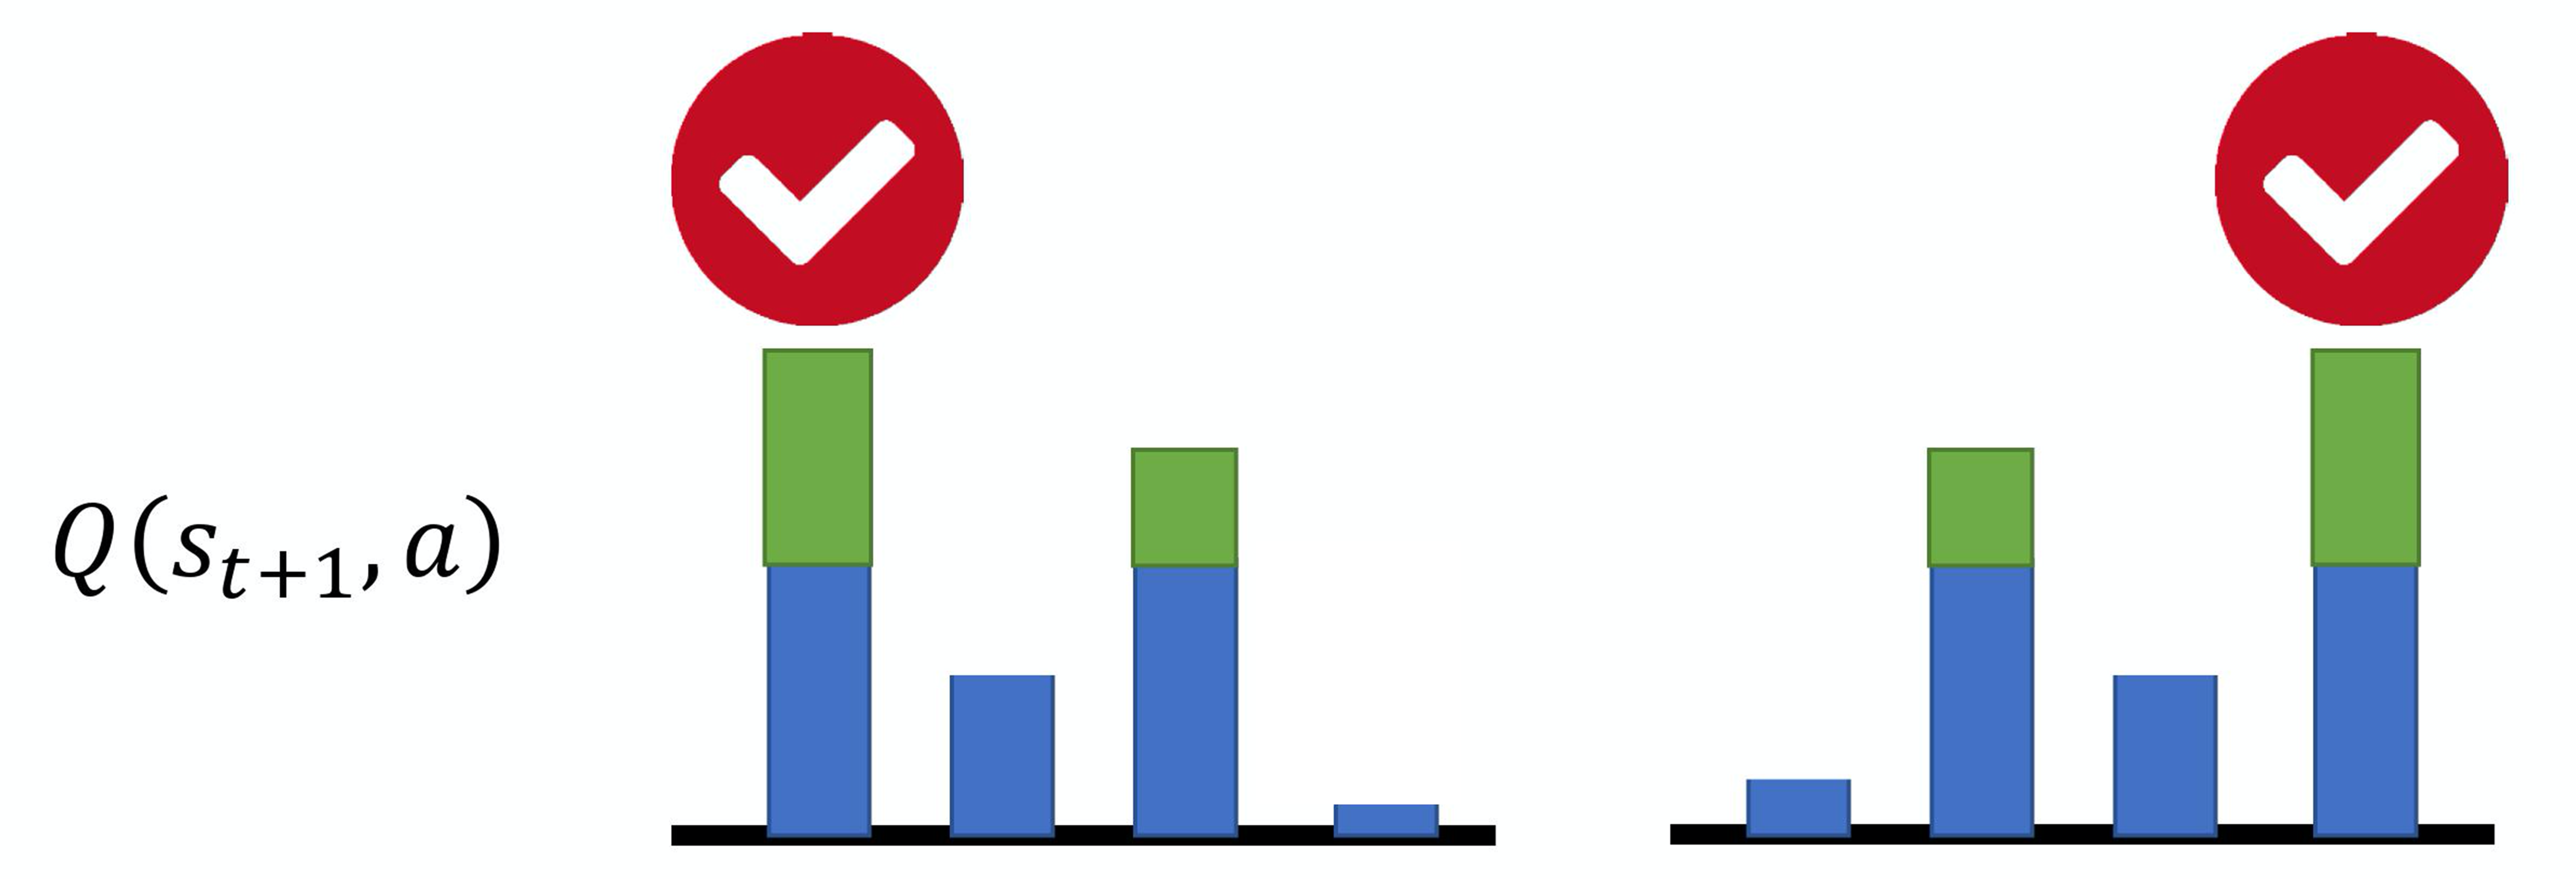
\includegraphics[width=0.5\linewidth]{res/ch7/7.2}
    \caption{Q值被高估的问题}
    \label{fig:double_dqn_1}
\end{figure}

% \begin{figure}[htb]
%     \centering
%     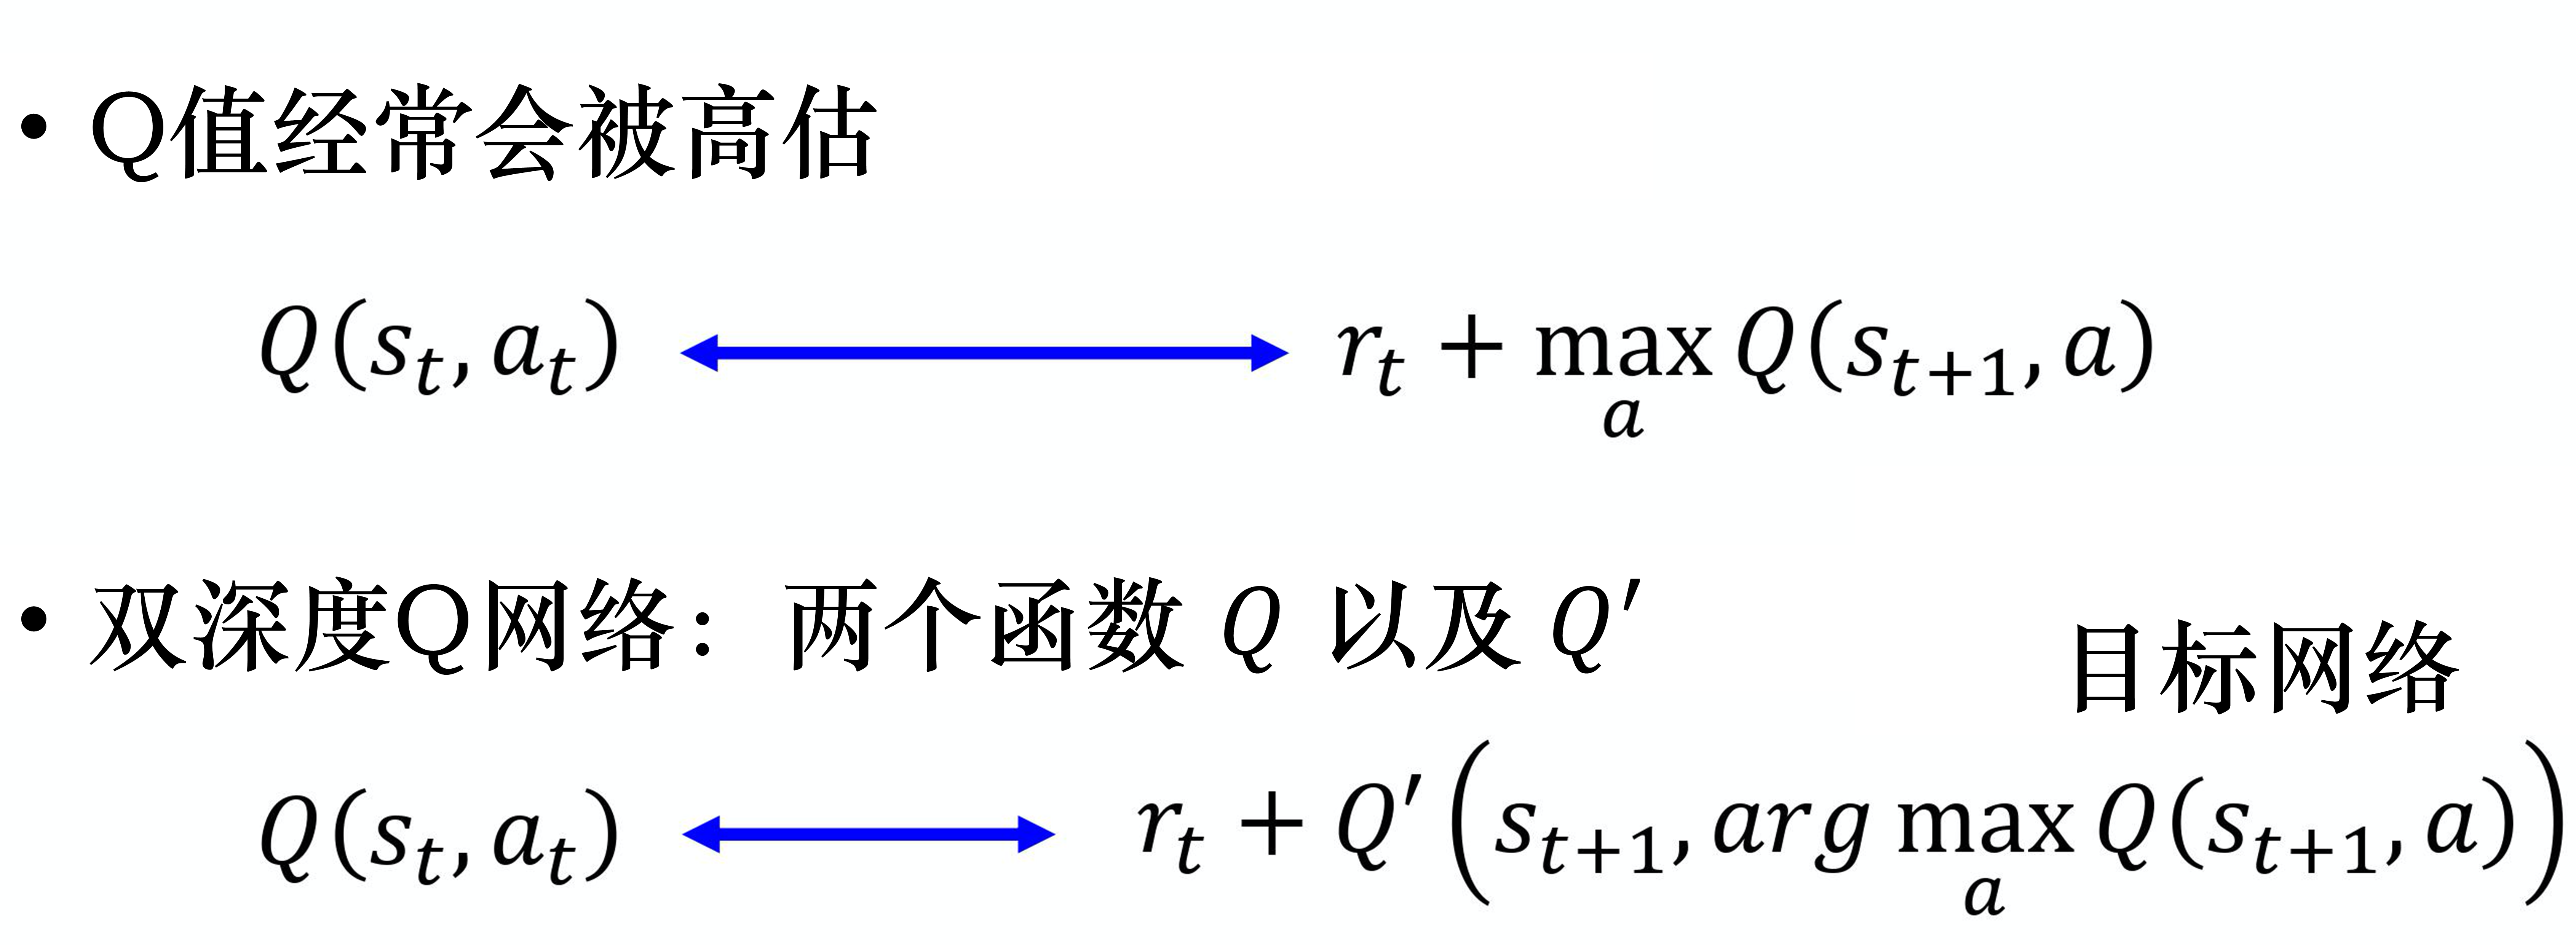
\includegraphics[width=0.5\linewidth]{res/ch7/7.3}
%     \caption{}
%     \label{fig:dobule_dqn_2}
% \end{figure}

Q: 怎么解决目标值总是太大的问题呢?

A: 在DDQN里面,选动作的Q函数与计算值的Q函数不是同一个。在原来的 深度Q网络 里面,我们穷举所有的 $a$,把每一个 $a$ 都代入Q函数,看哪一个 $a$ 可以得到的 Q 值最高,就把那个 Q 值加上 $r_t$。但是在 DDQN 里面有两个 Q网络,
    第一个 Q网络 Q 决定哪一个动作的 Q 值最大(我们把所有的 $a$ 代入 Q 函数中,看看哪一个 $a$ 的Q 值最大)。
    我们决定动作以后,Q 值是用 $Q'$ 算出来的。

如\eqref{eq:dobule_dqn_2} 所示,假设我们有两个Q函数------$Q$ 和 $Q'$,如果 $Q$ 高估了它选出来的动作 $a$,只要 $Q'$ 没有高估动作 $a$ 的值,算出来的就还是正常的值。
假设 $Q'$ 高估了某一个动作的值,也是没问题的,因为只要 $Q$ 不选这个动作就可以,这就是DDQN神奇的地方。

\begin{equation}
    \label{eq:dobule_dqn_2}
    Q\left(s_{t}, a_{t}\right) \longleftrightarrow r_{t}+Q^{\prime}\left(s_{t+1}, \arg \max _{a} Q\left(s_{t+1}, a\right)\right)
\end{equation}

我们动手实现的时候,有两个Q网络:会更新的Q网络和目标Q网络。所以在DDQN里面,我们会用会更新参数的Q网络去选动作,用目标Q网络(固定住的网络)计算值。

DDQN相较于原来的深度Q网络的更改是最少的,它几乎没有增加任何的运算量,也不需要新的网络,因为原来就有两个网络。我们只需要做一件事:本来是用目标网络 $Q'$ 来找使 Q 值最大的 $a$,现在改成用另外一个会更新的Q网络来找使 Q 值最大的 $a$。
如果只选一个技巧,我们一般都会选DDQN,因为其很容易实现。

\subsection{竞争深度Q网络} 
第二个技巧是\kw{竞争深度Q网络(dueling DQN)},相较于原来的 深度Q网络,它唯一的差别是改变了网络的架构。Q网络输入状态,输出的是每一个动作的 Q 值。
如\figref{fig:dueling_dqn_1} 所示,原来的深度Q网络直接输出 Q 值,竞争深度Q网络不直接输出 Q 值,而是分成两条路径运算。第一条路径会输出一个标量 $V(\boldsymbol{s})$,因为它与输入 $\boldsymbol{s}$ 是有关系的,所以称为 $V(\boldsymbol{s})$。
第二条路径会输出一个向量 $\boldsymbol{A}(\boldsymbol{s},\boldsymbol{a})$,它的每一个动作都有一个值。
我们再把 $V(\boldsymbol{s})$ 和 $\boldsymbol{A}(\boldsymbol{s},\boldsymbol{a})$ 加起来就可以得到 Q 值 $\boldsymbol{Q}(\boldsymbol{s},\boldsymbol{a})$。

\begin{figure}[htb]
    \centering
    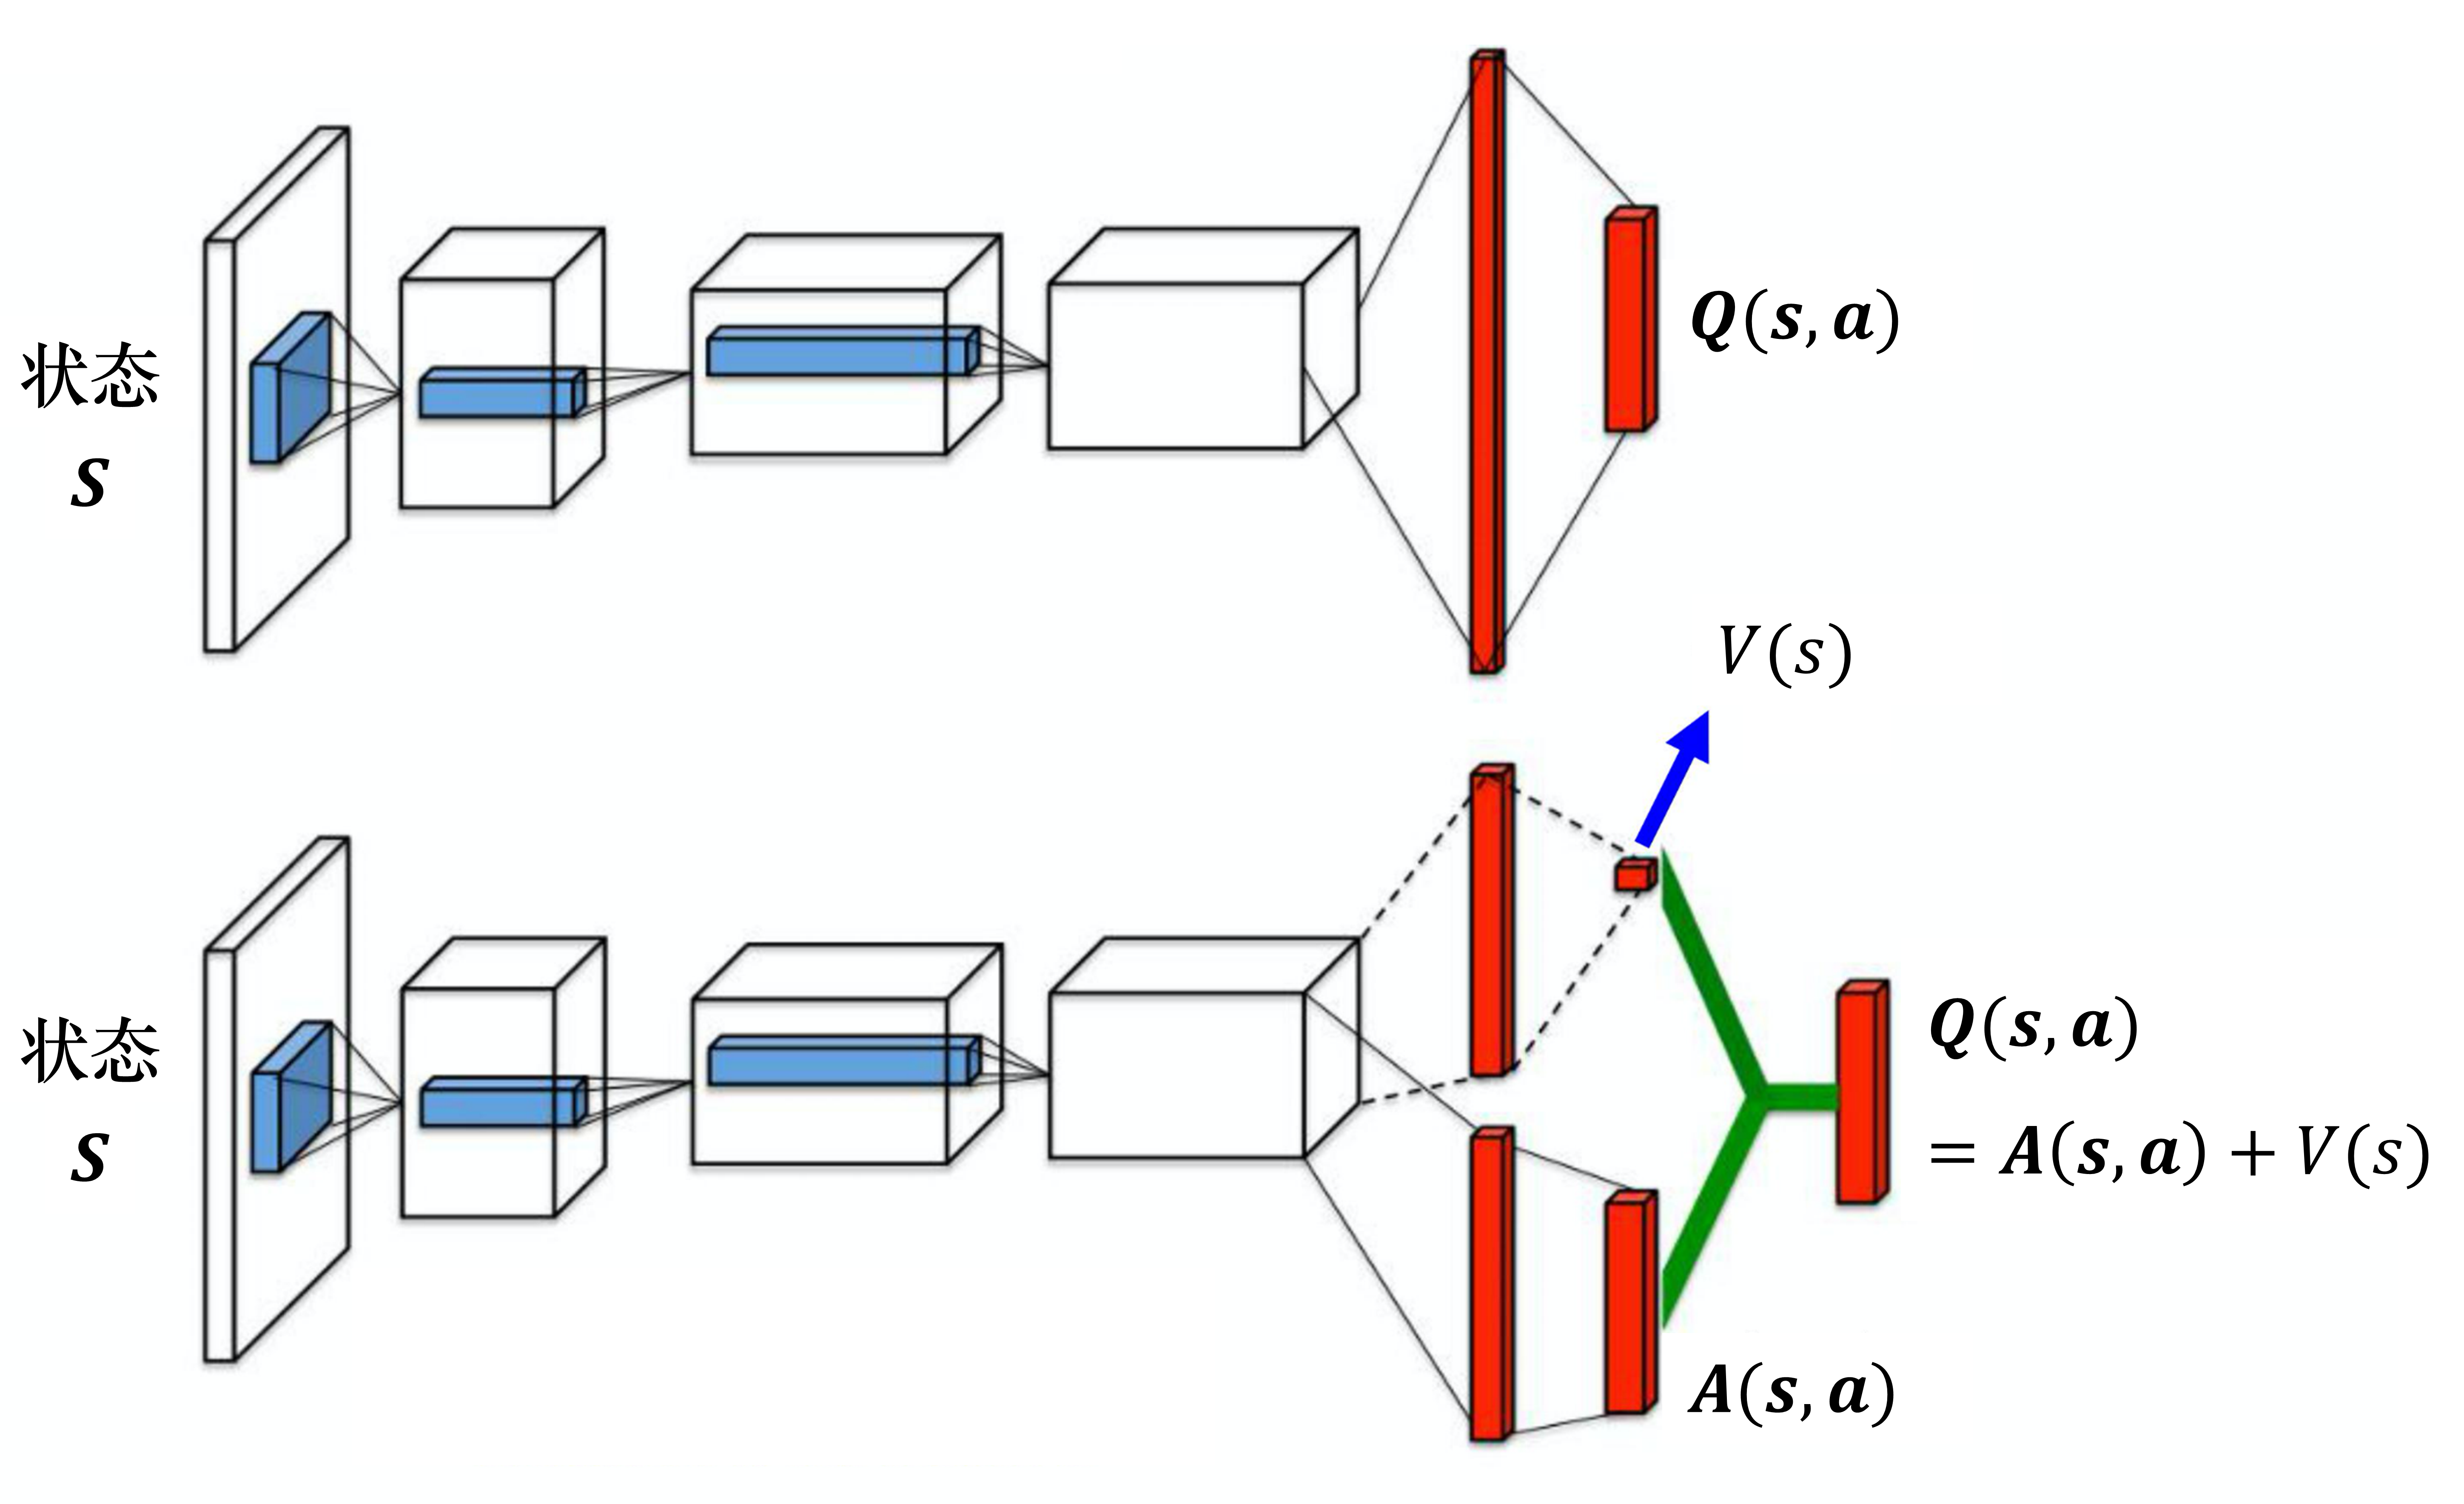
\includegraphics[width=0.5\linewidth]{res/ch7/7.4}
    \caption{竞争深度Q网络的网络结构\upcite{dueling_dqn_paper}}
    \label{fig:dueling_dqn_1}
\end{figure}

我们假设状态是离散的(实际上状态不是离散的),为了说明方便,我们假设就只有 4 个不同的状态,只有 3 个不同的动作,所以 $\boldsymbol{Q}(\boldsymbol{s},\boldsymbol{a})$  可以看成一个表格,如\figref{fig:dueling_dqn_2} 所示。

我们知道
$$
\boldsymbol{Q}(\boldsymbol{s},\boldsymbol{a}) = V(\boldsymbol{s}) + \boldsymbol{A}(\boldsymbol{s},\boldsymbol{a})
$$
其中,
$V(\boldsymbol{s})$ 对不同的状态,都有一个值。 
$\boldsymbol{A}(\boldsymbol{s},\boldsymbol{a})$ 对不同的状态、不同的动作都有一个值。
我们把 $V(\boldsymbol{s})$ 的每一列的值加到$\boldsymbol{A}(\boldsymbol{s},\boldsymbol{a})$的每一列就可以得到 Q 值,以第一列为例,有 2+1、2+($-$1)、2+0,可以得到 3、1、2,以此类推。

如\figref{fig:dueling_dqn_2} 所示,假设我们在训练网络的时候,目标是希望Q表格中第一行第二列的值变成 4,第二行第二列的值变成 0。但是我们实际上能修改的并不是 Q 值,能修改的是 $V(\boldsymbol{s})$ 与$\boldsymbol{A}(\boldsymbol{s},\boldsymbol{a})$的值。根据网络的参数,$V(\boldsymbol{s})$ 与$\boldsymbol{A}(\boldsymbol{s},\boldsymbol{a})$的值输出以后,就直接把它们加起来,所以其实不是修改 Q 值。
在学习网络的时候,假设我们希望 Q 表格中的 3 增加 1 变成 4、$-$1 增加 1 变成 0。最后我们在训练网络的时候,我们可能就不用修改 $\boldsymbol{A}(\boldsymbol{s},\boldsymbol{a})$的值,就修改 $V(\boldsymbol{s})$ 的值,把 $V(\boldsymbol{s})$ 的值从 0 变成 1。从 0 变成 1 有什么好处呢?本来只想修改两个值,但 Q表格中的第三个值也被修改了:$-$2 变成了 $-$1。
所以有可能我们在某一个状态下,只采样到这两个动作,没采样到第三个动作,但也可以更改第三个动作的 Q 值。这样的好处就是我们不需要把所有的状态-动作对都采样,可以用比较高效的方式去估计 Q 值。因为有时候我们更新的时候,不一定是更新Q表格,而是只更新了 $V(\boldsymbol{s})$,但更新 $V(\boldsymbol{s})$ 的时候,只要修改 $V(\boldsymbol{s})$的值,Q表格的值也会被修改。竞争深度Q网络是一个使用数据比较有效率的方法。

\begin{figure}[htb]
    \centering
    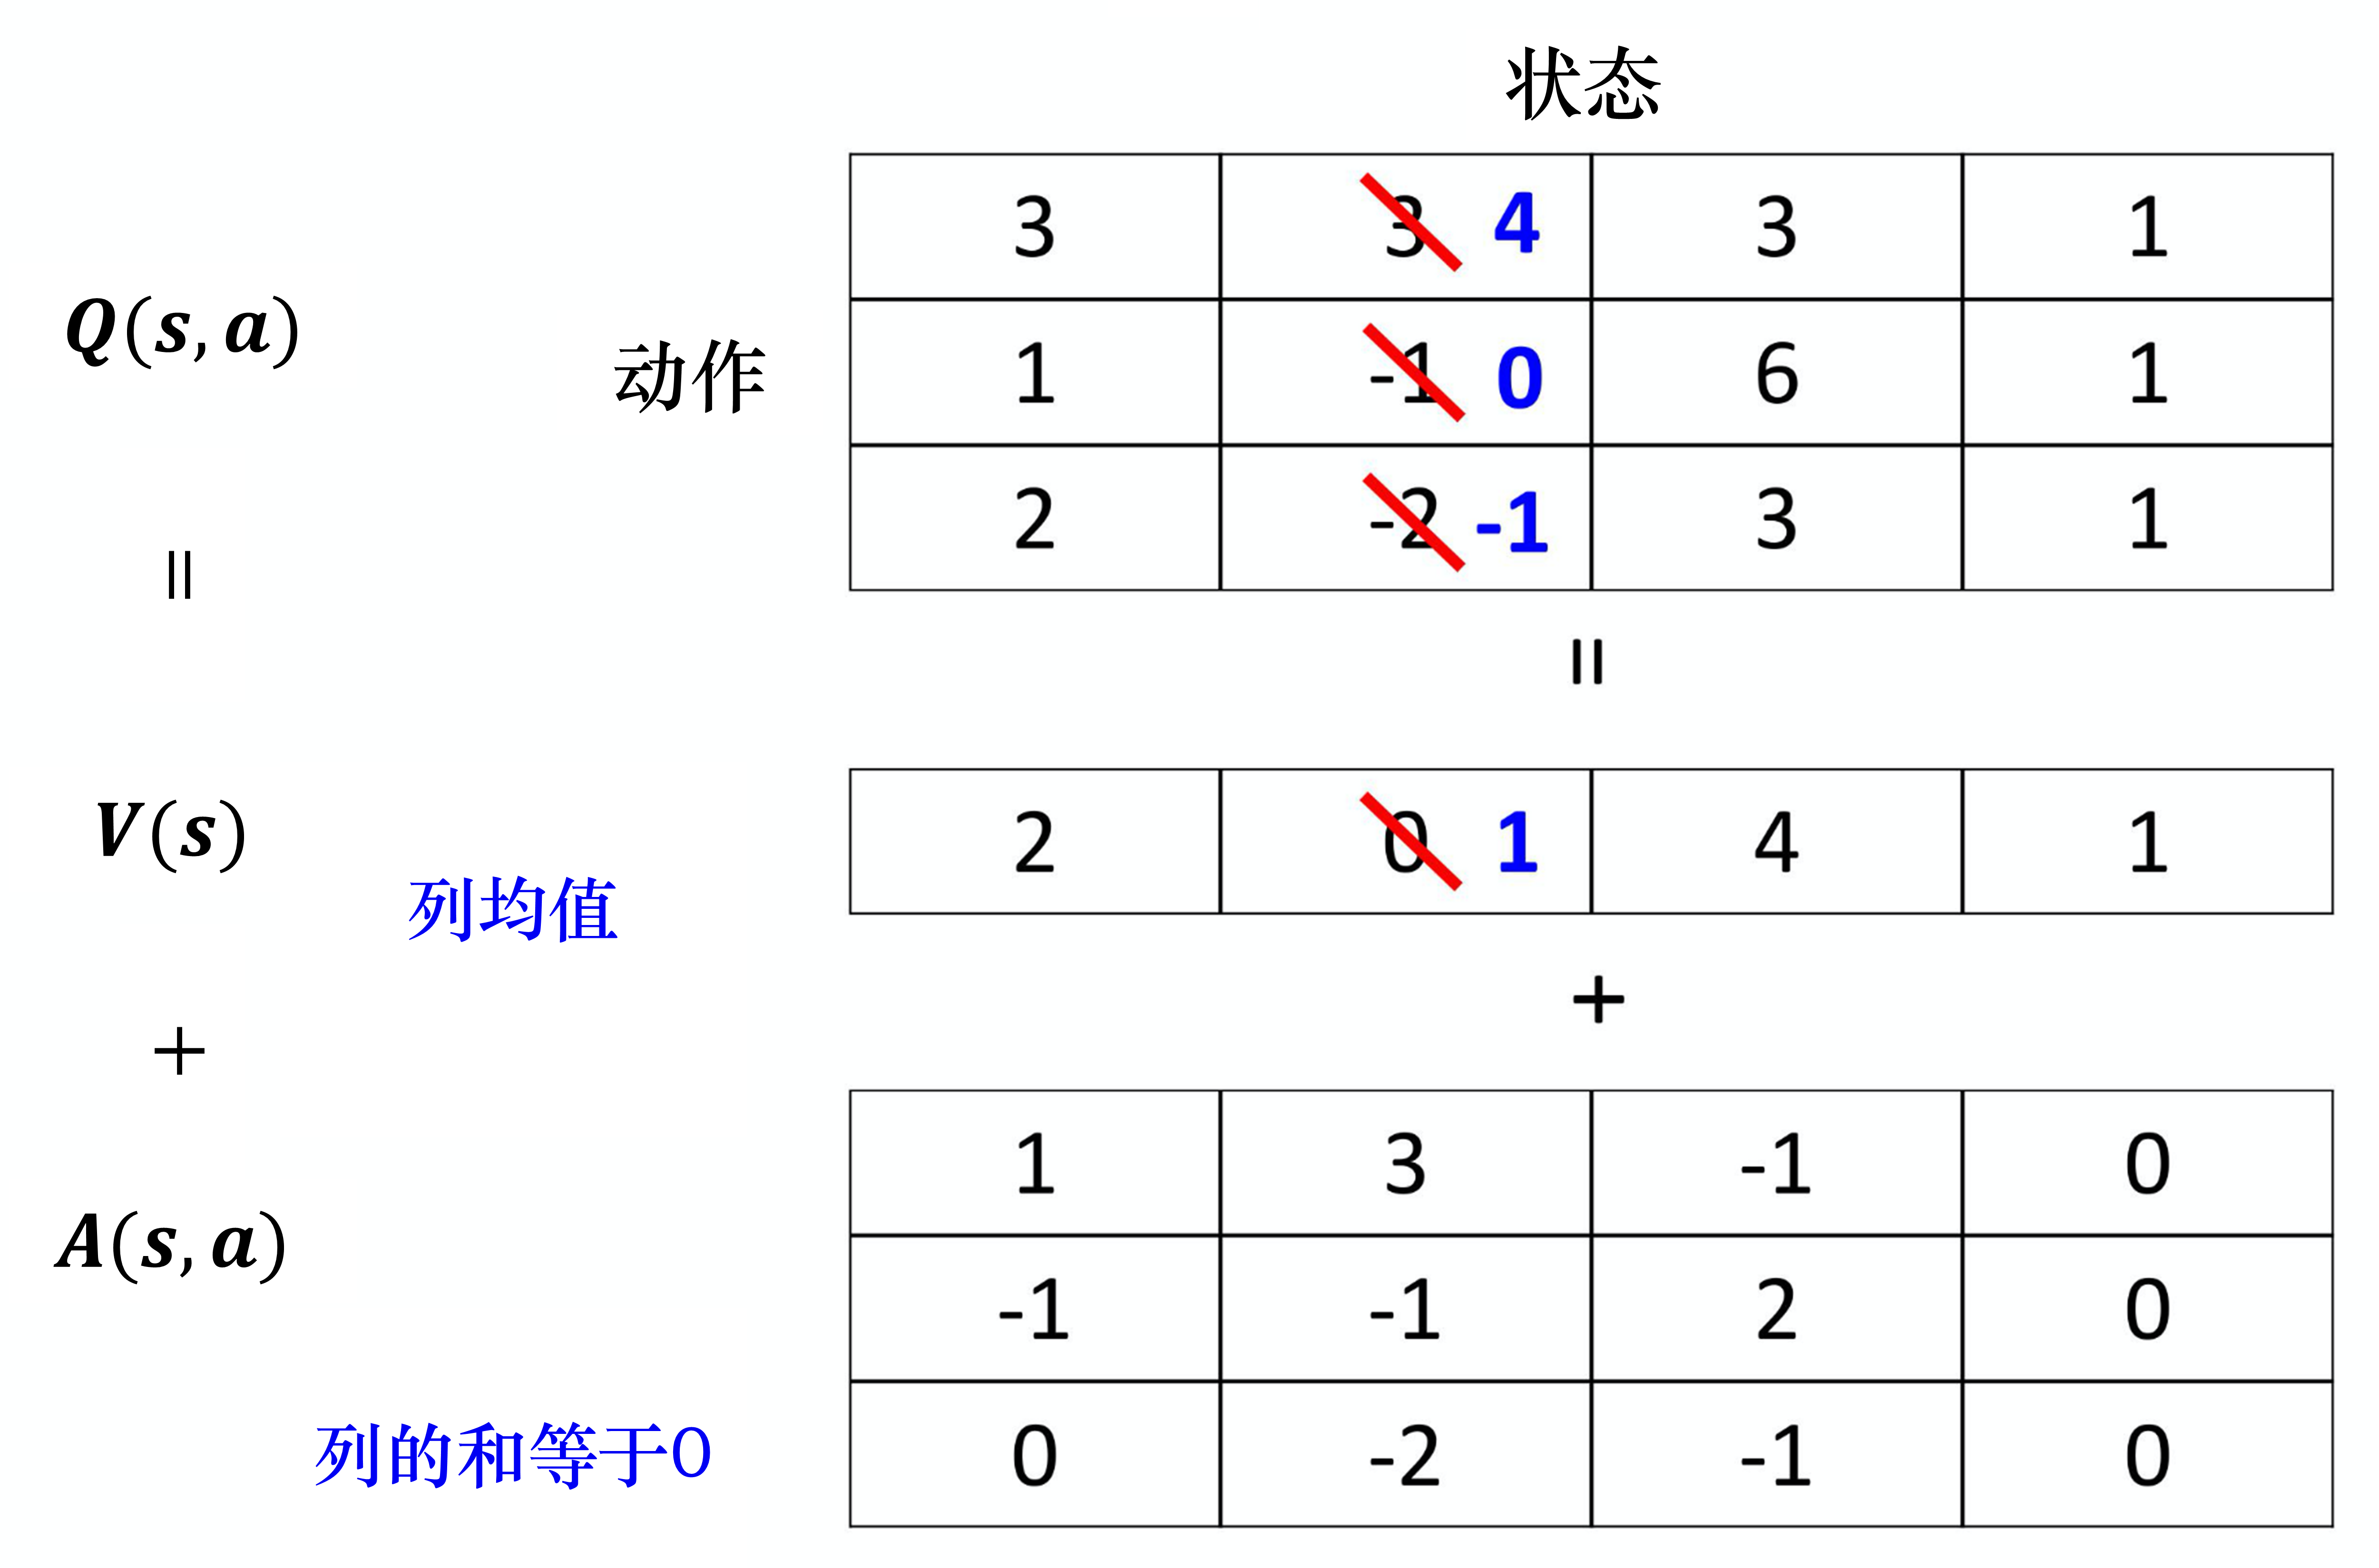
\includegraphics[width=0.5\linewidth]{res/ch7/7.5}
    \caption{竞争深度Q网络训练}
    \label{fig:dueling_dqn_2}
\end{figure}

可能会有人认为使用竞争深度Q网络会有一个问题,竞争深度Q网络最后学习的结果可能是这样的:智能体就学到 $V(\boldsymbol{s})$ 等于 0, $\boldsymbol{A}(\boldsymbol{s},\boldsymbol{a})$ 等于 Q,使用任何竞争深度Q网络就没有任何好处,就和原来的深度Q网络一样。
% 接下来有人就会问说会不会最后学习出来的结果是说,
为了避免这个问题出现,实际上我们要给 $\boldsymbol{A}(\boldsymbol{s},\boldsymbol{a})$ 一些约束,让 $\boldsymbol{A}(\boldsymbol{s},\boldsymbol{a})$的更新比较麻烦,让网络倾向于使用$V(\boldsymbol{s})$来解决问题。

例如,我们有不同的约束,一个最直觉的约束是必须要让 $\boldsymbol{A}(\boldsymbol{s},\boldsymbol{a})$ 的每一列的和都是 0,所以看我这边举的例子,列的和都是 0。如果这边列的和都是 0,我们就可以把$V(\boldsymbol{s})$的值想成是上面 Q 的每一列的平均值。这个平均值,加上$\boldsymbol{A}(\boldsymbol{s},\boldsymbol{a})$的值才会变成是 Q 的值。所以假设在更新参数的时候,要让整个列一起被更新,
更新  $\boldsymbol{A}(\boldsymbol{s},\boldsymbol{a})$ 的某一列比较麻烦,所以我们就不会想要更新 $\boldsymbol{A}(\boldsymbol{s},\boldsymbol{a})$ 的某一列。因为 $\boldsymbol{A}(\boldsymbol{s},\boldsymbol{a})$ 的每一列的和都要是 0,所以我们无法让$\boldsymbol{A}(\boldsymbol{s},\boldsymbol{a})$的某列的值都加1,这是做不到的,因为它的约束就是和永远都是 0,所以不可以都加1,这时候就会强迫网络去更新$V(\boldsymbol{s})$的值,让我们可以用比较有效率的方法去使用数据。

实现时,我们要给这个$\boldsymbol{A}(\boldsymbol{s},\boldsymbol{a})$一个约束。例如,如\figref{fig:dueling_dqn_3} 所示,假设有 3 个动作,输出的向量是 $[7,3,2]^{\mathrm{T}}$,我们在把 $\boldsymbol{A}(\boldsymbol{s},\boldsymbol{a})$与 $V(\boldsymbol{s})$ 加起来之前,先进行归一化(normalization)。
% 就类似层归一化(layer normalization)一样。
归一化的过程如下:

(1)计算均值(7+3+2)/3=4;

(2)向量$[7,3,2]^{\mathrm{T}}$的每个元素的值都减去均值4,于是归一化的向量为 $[3,-1,2]^{\mathrm{T}}$。

接着我们将向量$[3,-1,2]^{\mathrm{T}}$中的每个元素的值加上 1,就可以得到最后的 Q 值。这个归一化的步骤就是网络的其中一部分,在训练的时候,我们也使用反向传播,只是归一化是没有参数的,它只是一个操作,可以把它放到网络里面,与网络的其他部分共同训练,这样$\boldsymbol{A}(\boldsymbol{s},\boldsymbol{a})$就会有比较大的约束,网络就会给它一些好处,让它倾向于去更新$V(\boldsymbol{s})$的值,这就是竞争深度Q网络。
\begin{figure}[htb]
    \centering
    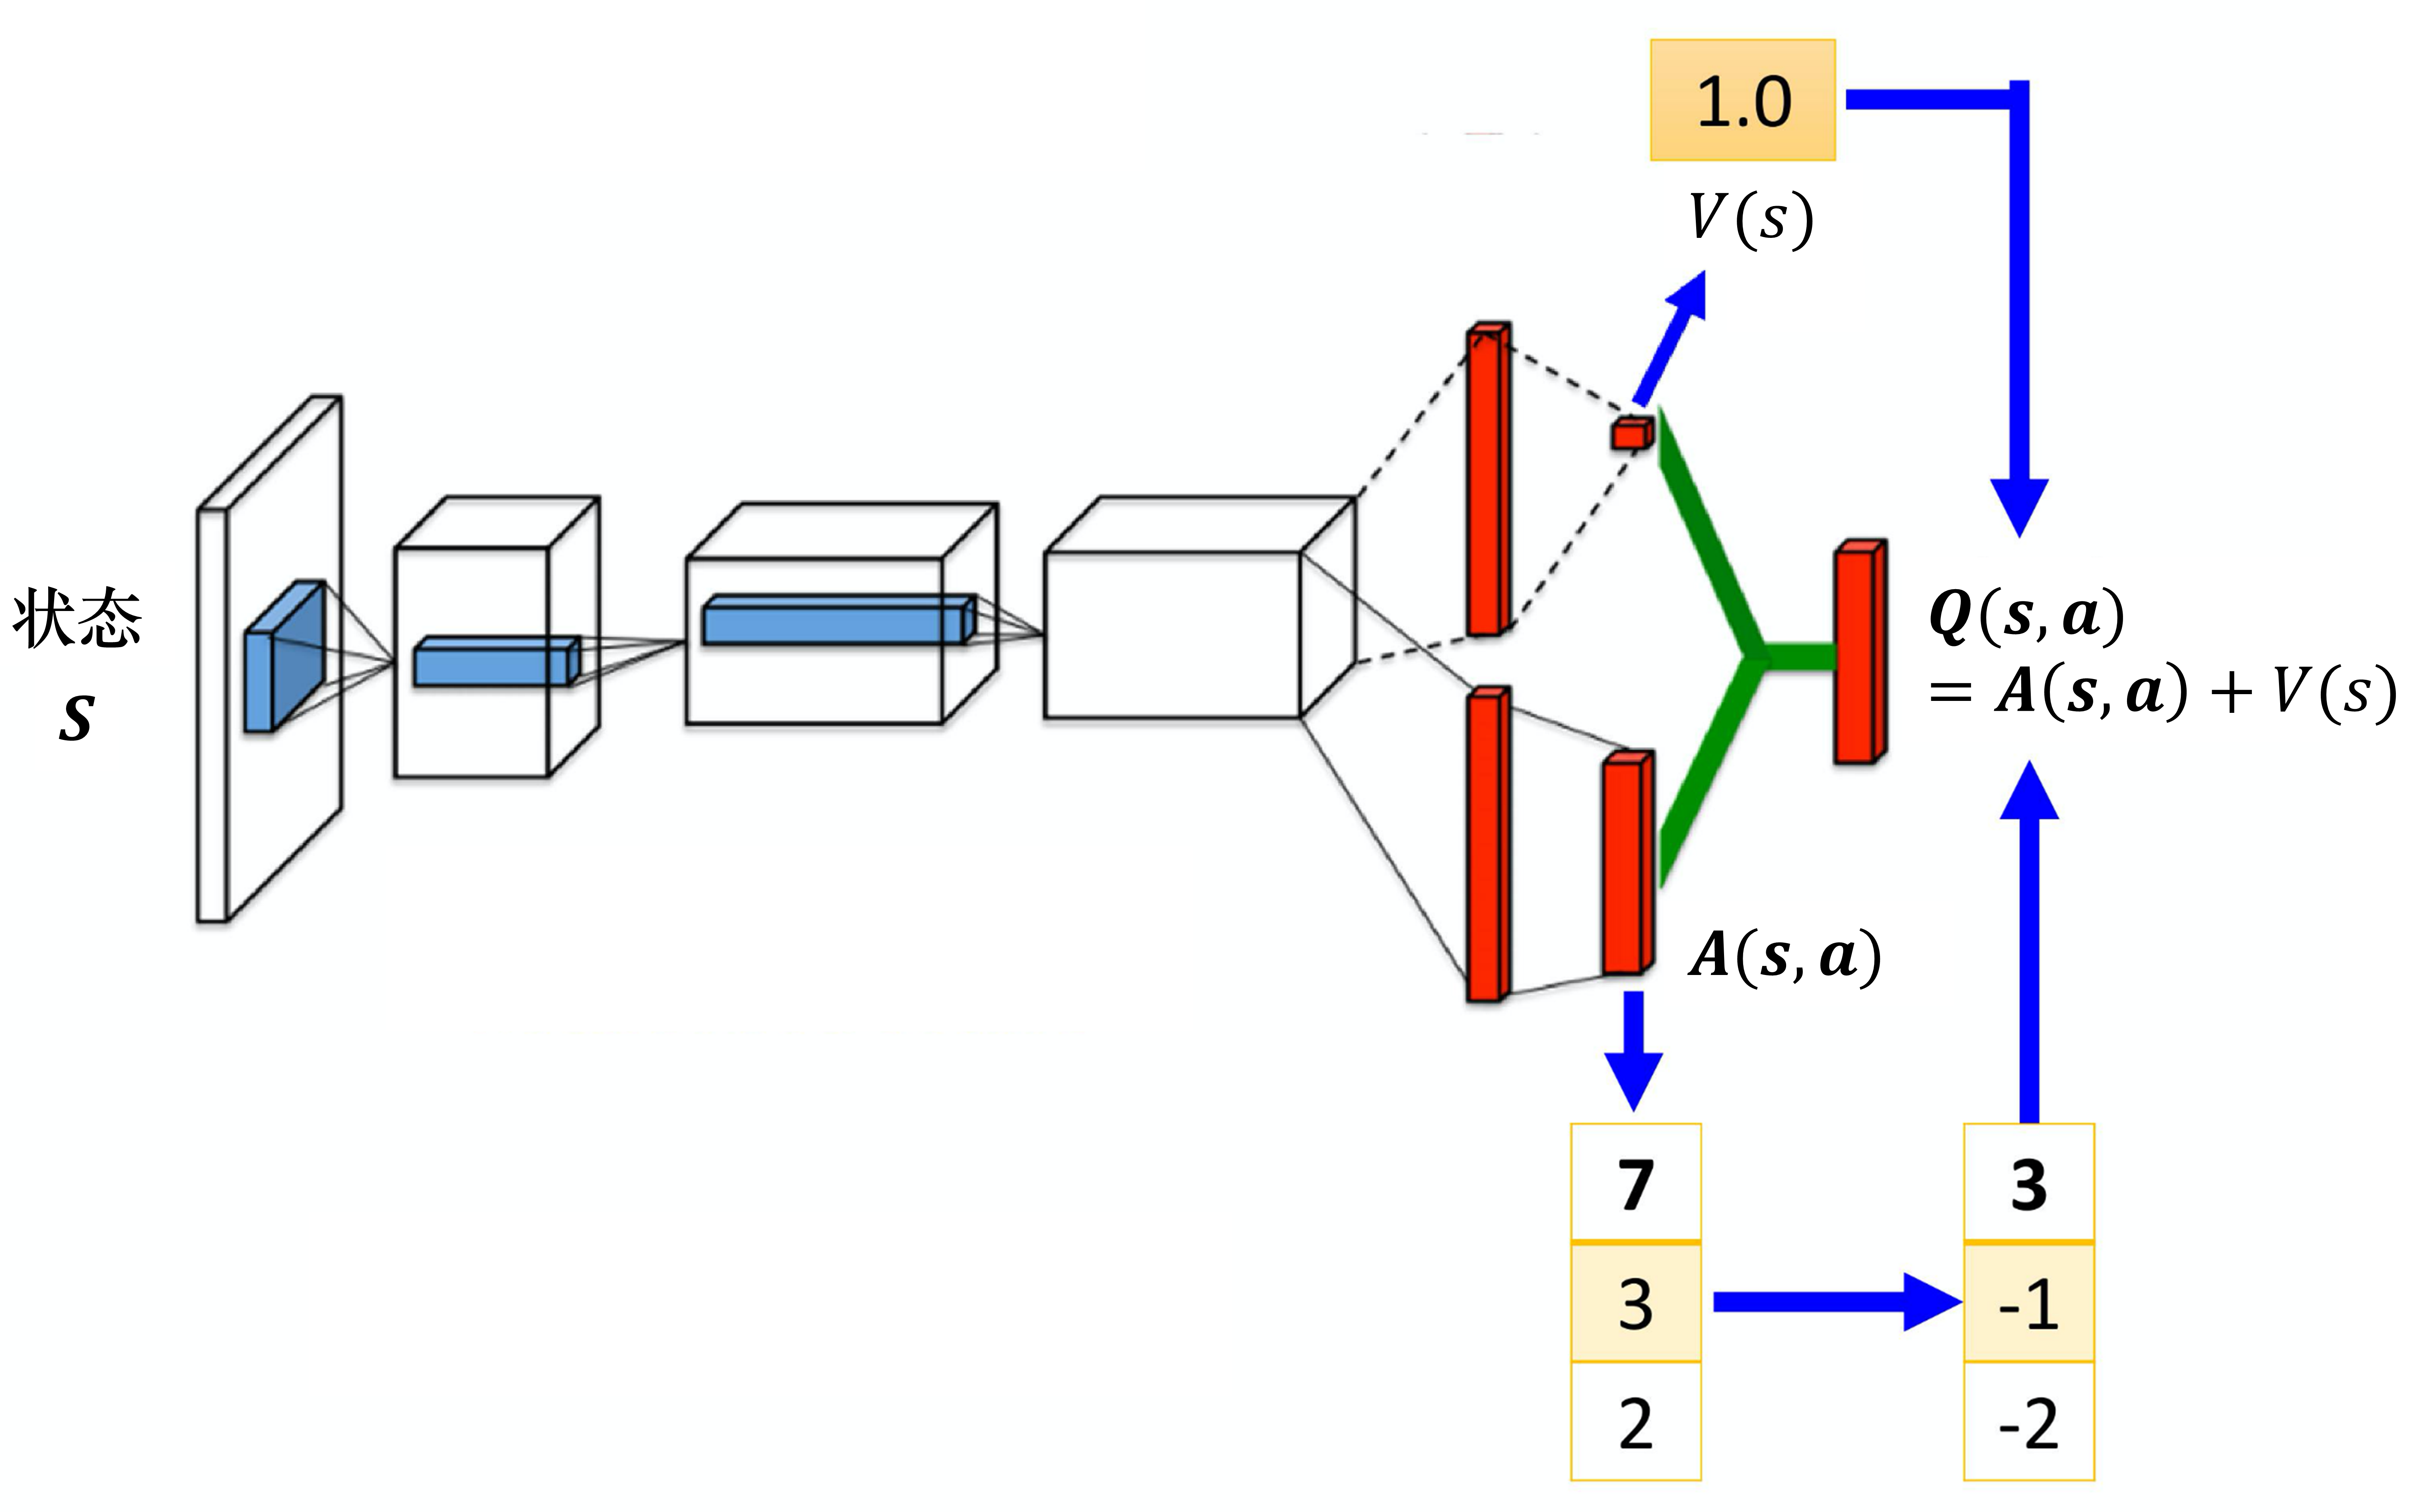
\includegraphics[width=0.5\linewidth]{res/ch7/7.6}
    \caption{竞争深度Q网络约束\upcite{dueling_dqn_paper}}
    \label{fig:dueling_dqn_3}
\end{figure}

\subsection{优先级经验回放} 

第三个技巧称为\kw{优先级经验回放(prioritized experience replay,PER)}。
如\figref{fig:PER} 所示,我们原来在采样数据训练 Q 网络的时候,会均匀地从回放缓冲区里面采样数据。这样不一定是最好的, 因为也许有一些数据比较重要。假设有一些数据,我们之前采样过,发现这些数据的时序差分误差特别大(时序差分误差就是网络的输出与目标之间的差距),这代表我们在训练网络的时候,这些数据是比较不好训练的。既然比较不好训练,就应该给它们比较大的概率被采样到,即给它\kw{优先权(priority)}。这样在训练的时候才会多考虑那些不好训练的数据。实际上在做 PER 的时候,我们不仅会更改采样的过程,还会因为更改了采样的过程,而更改更新参数的方法。所以PER不仅改变了采样数据的分布,还改变了训练过程。

\begin{figure}[htb]
    \centering
    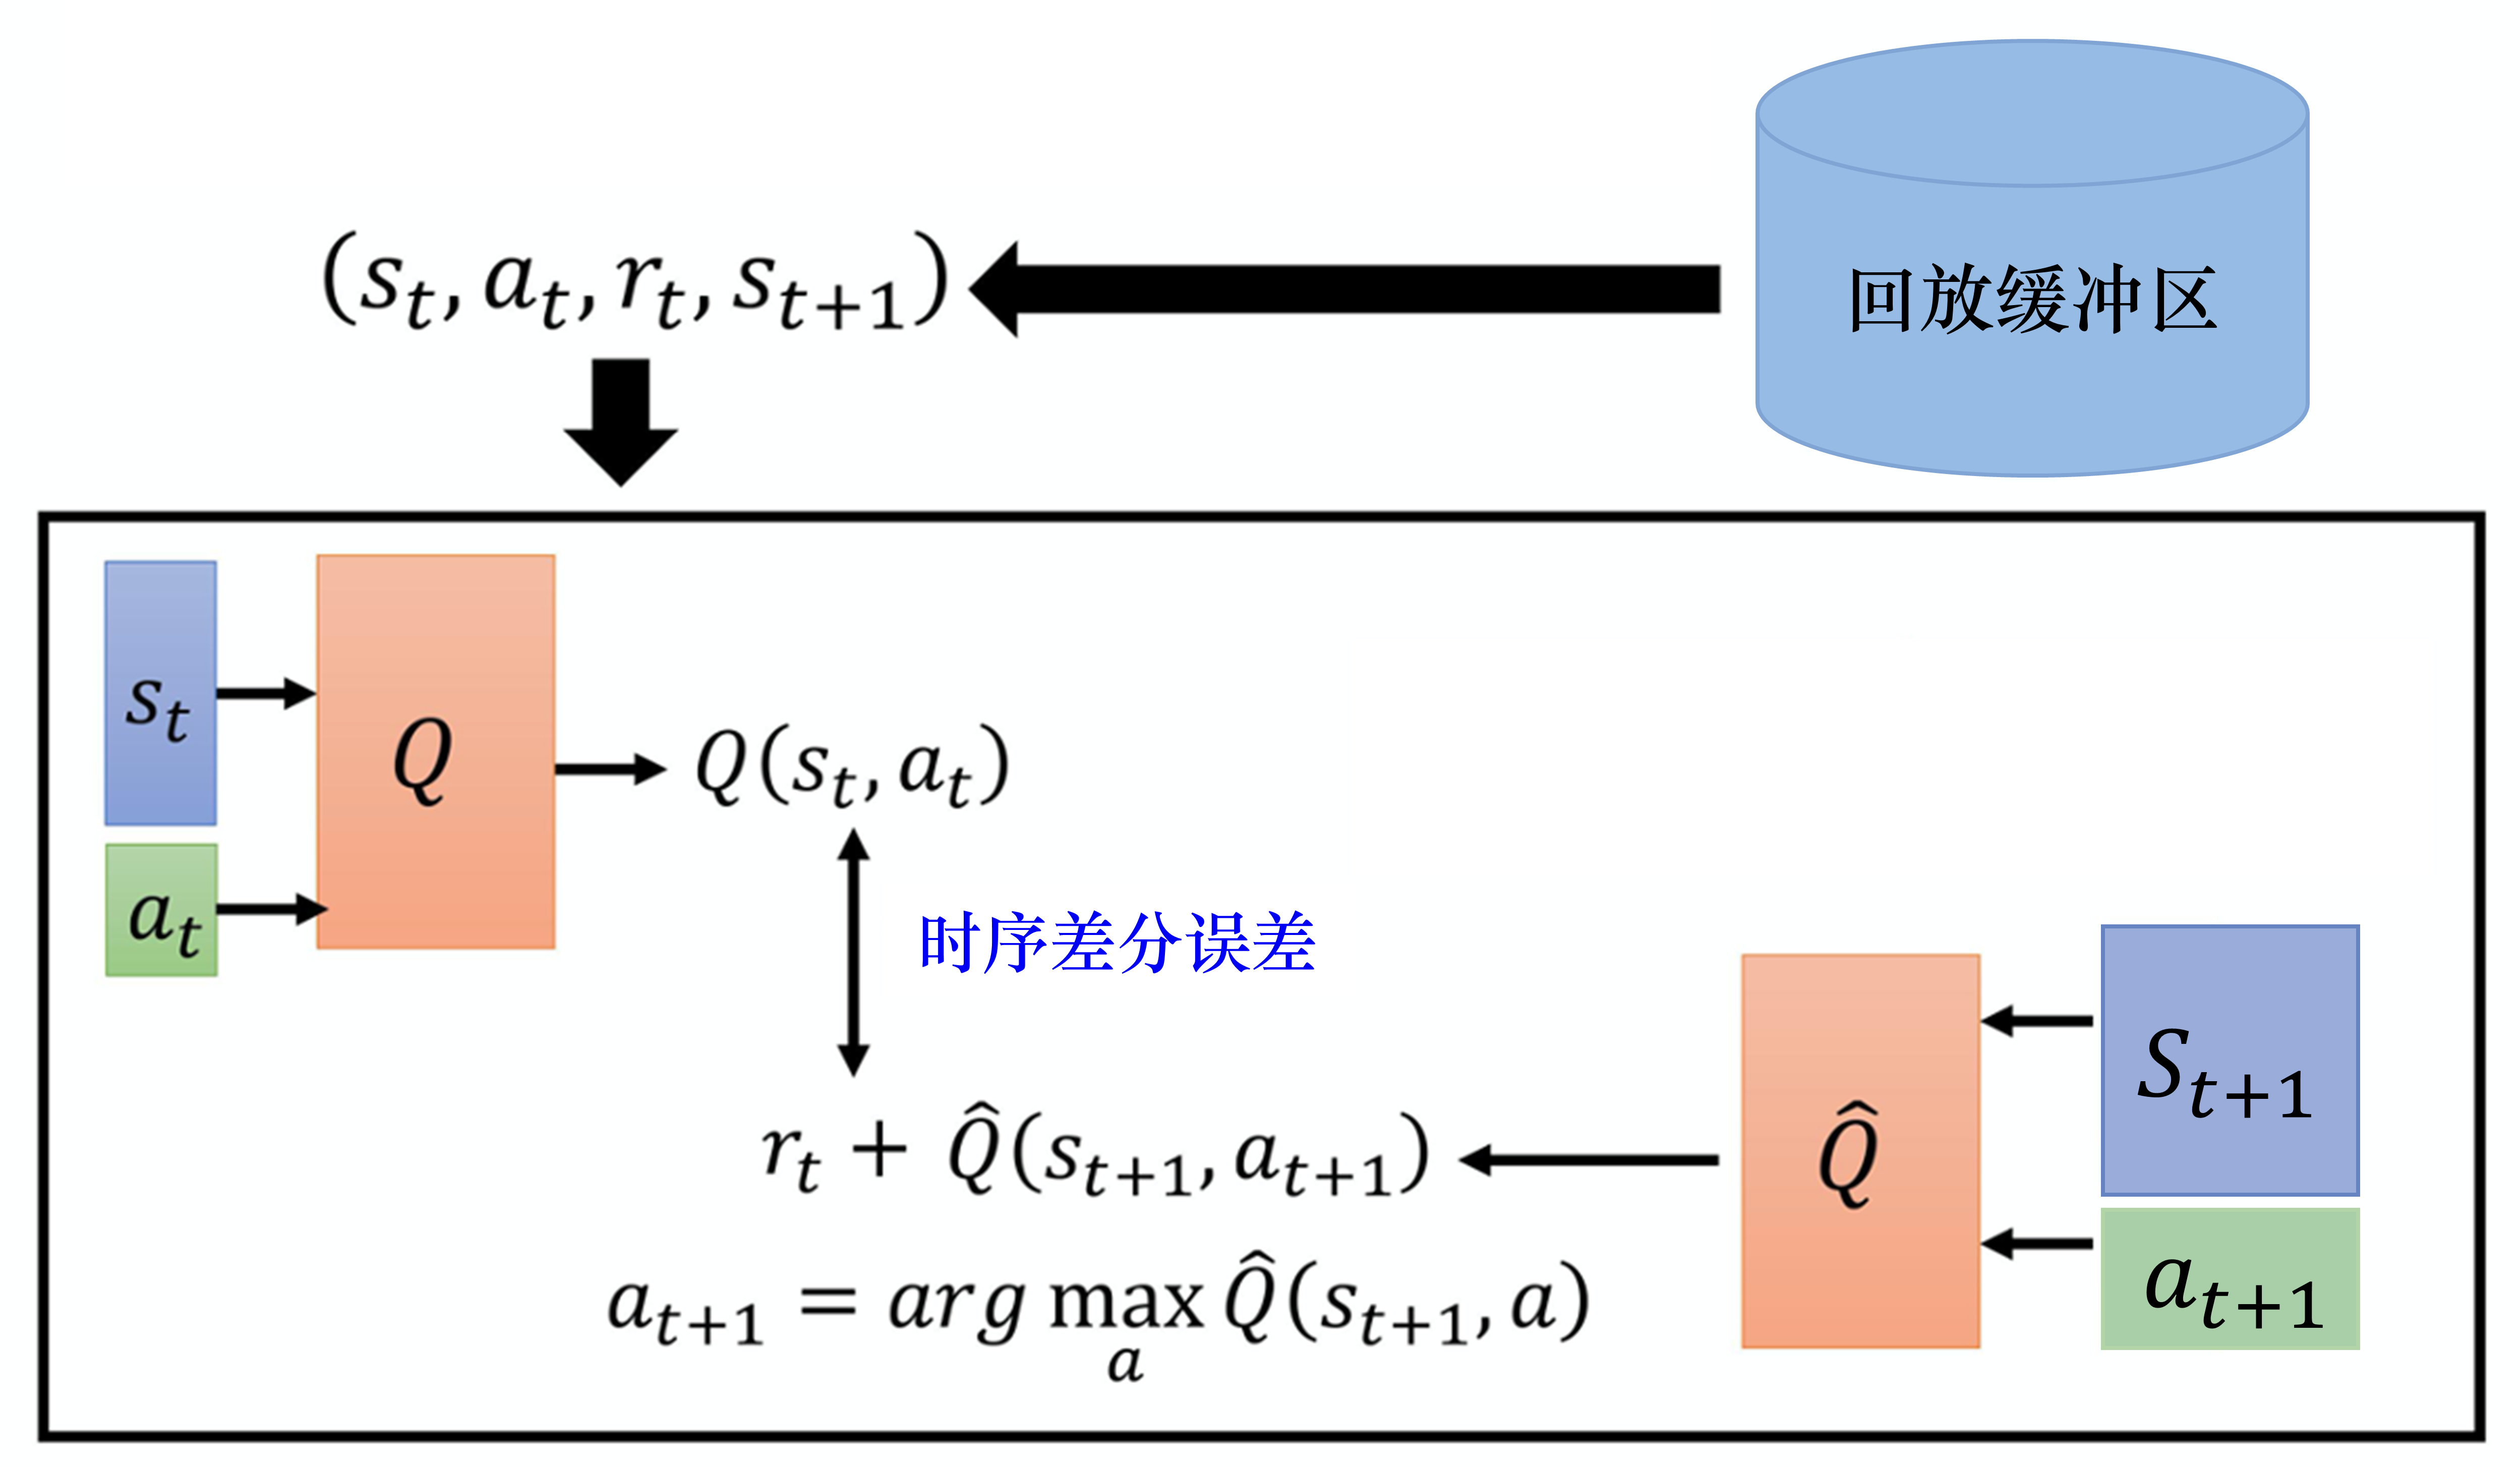
\includegraphics[width=0.5\linewidth]{res/ch7/7.7}
    \caption{优先级经验回放}
    \label{fig:PER}
\end{figure}

\subsection{在蒙特卡洛方法和时序差分方法中取得平衡} 
蒙特卡洛方法与时序差分方法各有优劣,因此我们可以在蒙特卡洛方法和时序差分方法中取得平衡,这个方法也被称为多步方法。我们的做法如\figref{fig:balance_MC_TD} 所示,在时序差分方法里面,在某一个状态 $s_t$ 采取某一个动作$a_t$ 得到奖励 $r_t$,接下来进入状态 $s_{t+1}$。但是我们可以不只保存一个步骤的数据,可保存 $N$ 个步骤的数据。

我们记录在 $s_t$ 采取 $a_t$,得到 $r_t$时,会进入的 $s_{t+1}$。一直记录到第 $N$ 个步骤以后,在 $s_{t+N}$采取 $a_{t+N}$,得到 $r_{t+N}$,进入 $s_{t+N+1}$ 的这些经验,把它们保存下来。实际上在做更新的时候,在做Q网络学习的时候,我们要让 $Q(s_t,a_t)$ 与目标值越接近越好。$\hat{Q}$ 所计算的不是 $s_{t+1}$的,而是 $s_{t+N+1}$的奖励。我们会把 $N$ 个步骤以后的状态$s_{t+N+1}$ 输入到 $\hat{Q}$ 中去计算 $N$ 个步骤以后会得到的奖励。如果要算目标值,要再加上多步(multi-step)的奖励 $\sum_{t^{\prime}=t}^{t+N} r_{t^{\prime}}$ ,多步的奖励是从时间 $t$ 一直到 $t+N$ 的 $N+1$ 个奖励的和。我们希望 $Q(s_t,a_t)$ 和目标值越接近越好。

多步方法就是蒙特卡洛方法与时序差分方法的结合,因此它不仅有蒙特卡洛方法的好处与坏处,还有时序差分方法的好处与坏处。我们先看看多步方法的好处,之前只采样了某一个步骤,所以得到的数据是真实的,接下来都是 Q 值估测出来的。现在采样比较多的步骤,采样 $N$ 个步骤才估测值,所以估测的部分所造成的影响就会比较小。
当然多步方法的坏处就与蒙特卡洛方法的坏处一样,因为 $r$ 有比较多项,所以我们把 $N$ 项的 $r$ 加起来,方差就会比较大。但是我们可以调整 $N$ 的值,在方差与不精确的 Q 值之间取得一个平衡。$N$ 就是一个超参数,我们可以对其进行调整。

\begin{figure}[htb]
    \centering
    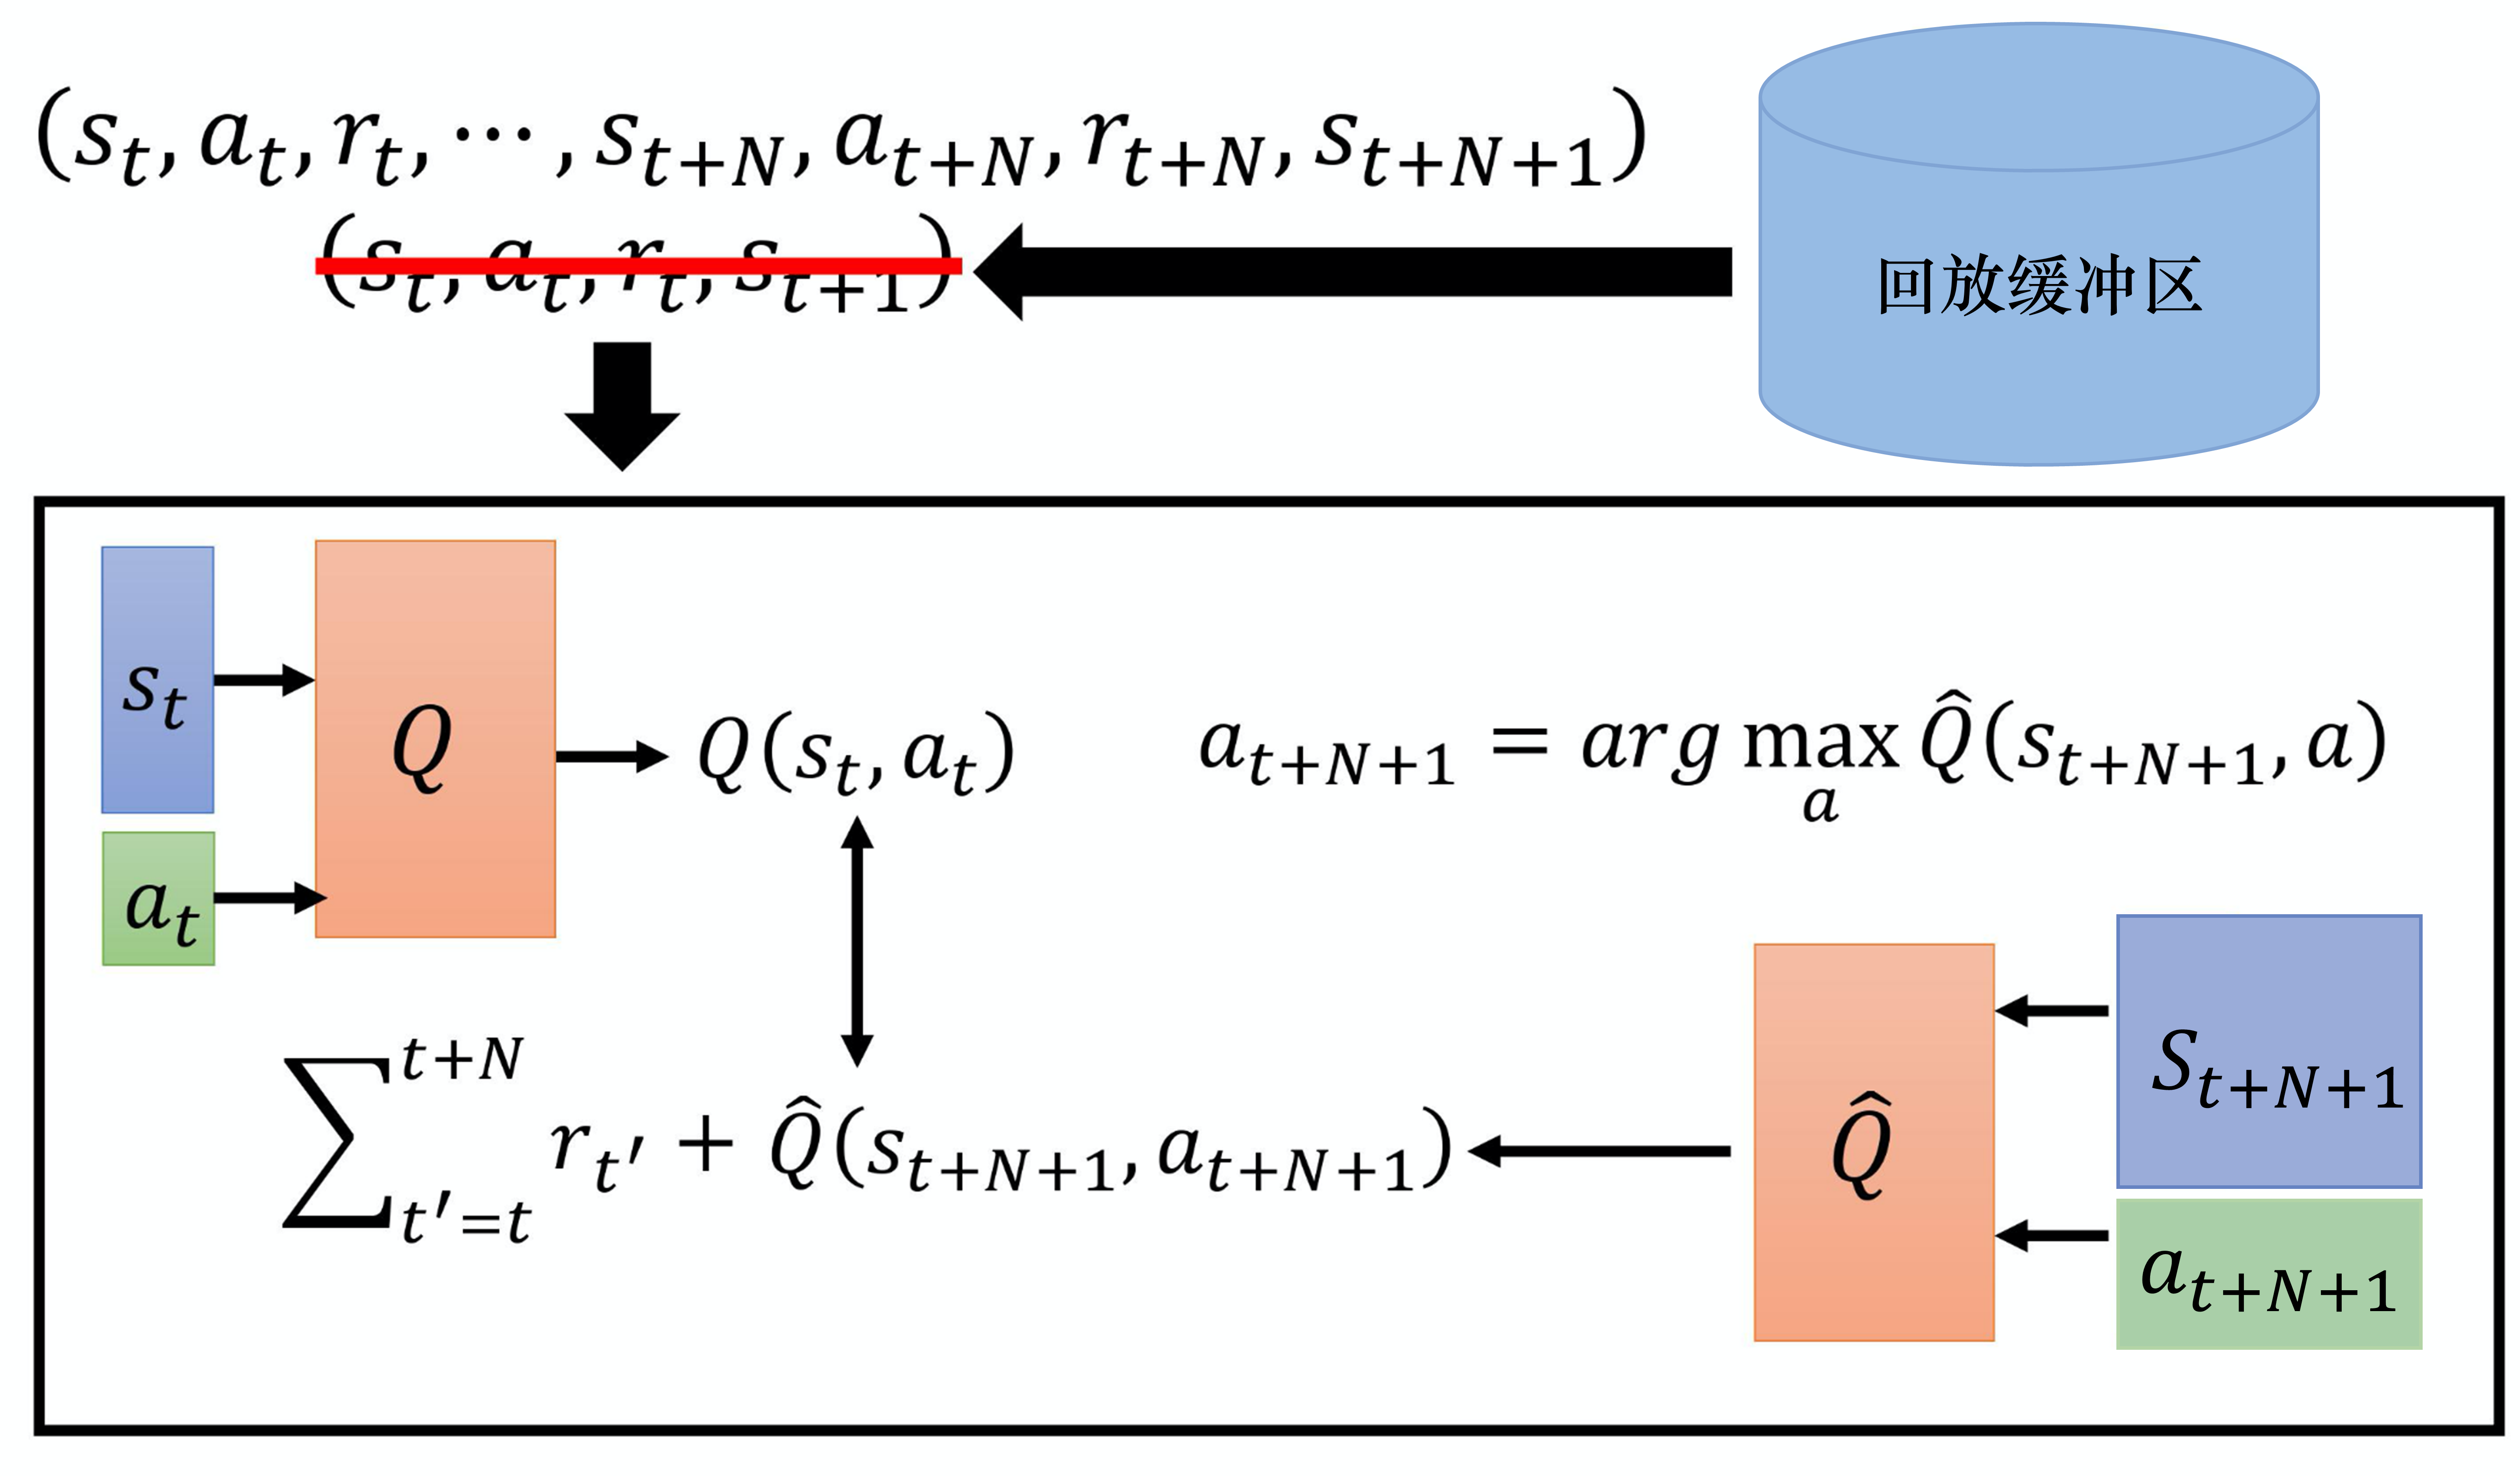
\includegraphics[width=0.5\linewidth]{res/ch7/7.8}
    \caption{在蒙特卡洛方法和时序差分方法中取得平衡}
    \label{fig:balance_MC_TD}
\end{figure}

\subsection{噪声网络} 
% \begin{figure}[htb]
%     \centering
%     \includegraphics[width=0.5\linewidth]{res/ch7/7.9}
%     \caption{}
%     \label{fig:}
% \end{figure}

我们还可以改进探索。$\varepsilon$-贪心这样的探索就是在动作的空间上加噪声,但是有一个更好的方法称为\kw{噪声网络(noisy net)},它是在参数的空间上加噪声。
噪声网络是指,每一次在一个回合开始的时候,在智能体要与环境交互的时候,智能体使用Q函数来采取动作,Q函数里面就是一个网络,我们在网络的每一个参数上加上一个高斯噪声(Gaussian noise),就把原来的Q函数变成 $\tilde{Q}$ 。因为我们已经用 $\hat{Q}$ 来表示目标网络,所以我们用 $\tilde{Q}$  来表示\kw{噪声Q函数(noisy Q-function)}。我们把每一个参数都加上一个高斯噪声,就得到一个新的网络 $\tilde{Q}$。使用噪声网络执行的动作为
\begin{equation}
    \label{eq:}
    a=\underset{a}{\arg \max} \tilde{Q}(s, a)
\end{equation}

这里要注意,在每个回合开始的时候,与环境交互之前,我们就采样噪声。接下来我们用固定的噪声网络玩游戏,直到游戏结束,才重新采样新的噪声,噪声在一个回合中是不能被改变的。
OpenAI 与 DeepMind 在同时间提出了几乎一模一样的噪声网络方法,并且对应的两篇论文都发表在 ICLR 2018 会议中。不一样的地方是,他们用不同的方法加噪声。OpenAI 的方法比较简单,直接加一个高斯噪声,也就是把每一个参数、每一个权重(weight)都加一个高斯噪声。DeepMind 的方法比较复杂,该方法中的噪声是由一组参数控制的,网络可以自己决定噪声要加多大。但是两种方法的概念都是一样的,总之,我们就是对Q函数里面的网络加上一些噪声,把它变得有点儿不一样,即与原来的Q函数不一样,然后与环境交互。两篇论文里面都强调,参数虽然会被加上噪声,但在同一个回合里面参数是固定的。我们在换回合、玩另一场新的游戏的时候,才会重新采样噪声。在同一场游戏里面就是同一个噪声Q网络在玩该场游戏,这非常重要。因为这导致了噪声网络与原来的$\varepsilon$-贪心或其他在动作上做采样的方法的本质上的差异。

% \begin{figure}[htb]
%     \centering
%     \includegraphics[width=0.5\linewidth]{res/ch7/7.10}
%     \caption{}
%     \label{fig:}
% \end{figure}

有什么本质上的差异呢?在原来采样的方法中,比如$\varepsilon$-贪心中,就算给定同样的状态,智能体采取的动作也不一定是一样的。因为智能体通过采样来决定动作,给定同一个状态,智能体根据Q函数的网络来输出一个动作,或者采样到随机来输出一个动作。所以给定相同的状态,如果是用$\varepsilon$-贪心的方法,智能体可能会执行不同的动作。
但实际上策略并不是这样的,一个真实世界的策略,给定同样的状态,它应该有同样的回应。而不是给定同样的状态,它有时候执行Q函数,有时候又是随机的,这是一个不正常的动作,是在真实的情况下不会出现的动作。
但是如果我们是在Q函数的网络的参数上加噪声, 就不会出现这种情况。
因为如果在Q函数的网络的参数上加噪声,在整个交互的过程中,在同一个回合里面,它的网络的参数总是固定的,所以看到相同或类似的状态,就会采取相同的动作,这是比较正常的。这被称为\kw{依赖状态的探索(state-dependent exploration)},我们虽然会做探索这件事,但是探索是与状态有关系的,看到同样的状态,就会采取同样的探索的方式,而噪声(noisy)的动作只是随机乱试。但如果我们是在参数下加噪声,在同一个回合里面,参数是固定的,我们就是系统地尝试。比如,我们每次在某一个状态,都向左试试看。在下一次在玩同样游戏的时候,看到同样的状态,我再向右试试看,是系统地在探索环境。

\subsection{分布式Q函数} 
还有一个技巧称为\kw{分布式Q函数(distributional Q-function)}。分布式Q函数是比较合理的,但是它难以实现。Q函数是累积奖励的期望值,所以我们算出来的 Q 值其实是一个期望值。
如\figref{fig:fig7.11} 所示,
因为环境是有随机性的,所以在某一个状态采取某一个动作的时候,我们把所有的奖励在游戏结束的时候进行统计,得到的是一个分布。也许在奖励得到 0 的概率很高,得到 $-$10 的概率比较低,得到 +10 的概率也比较低,但是它是一个分布。(我们对这个分布计算它的平均值才是这个 Q 值,算出来是累积奖励的期望。所以累积奖励是一个分布,对它取期望,对它取平均值,得到 Q 值)。
但不同的分布可以有同样的平均值。也许真正的分布是\figref{fig:fig7.11} 所示右边的分布,它的平均值与左边的分布的平均值其实是一样的,但它们背后所代表的分布其实是不一样的。假设我们只用 Q 值的期望来代表整个奖励,可能会丢失一些信息,无法对奖励的分布进行建模。

\begin{figure}[htb]
    \centering
    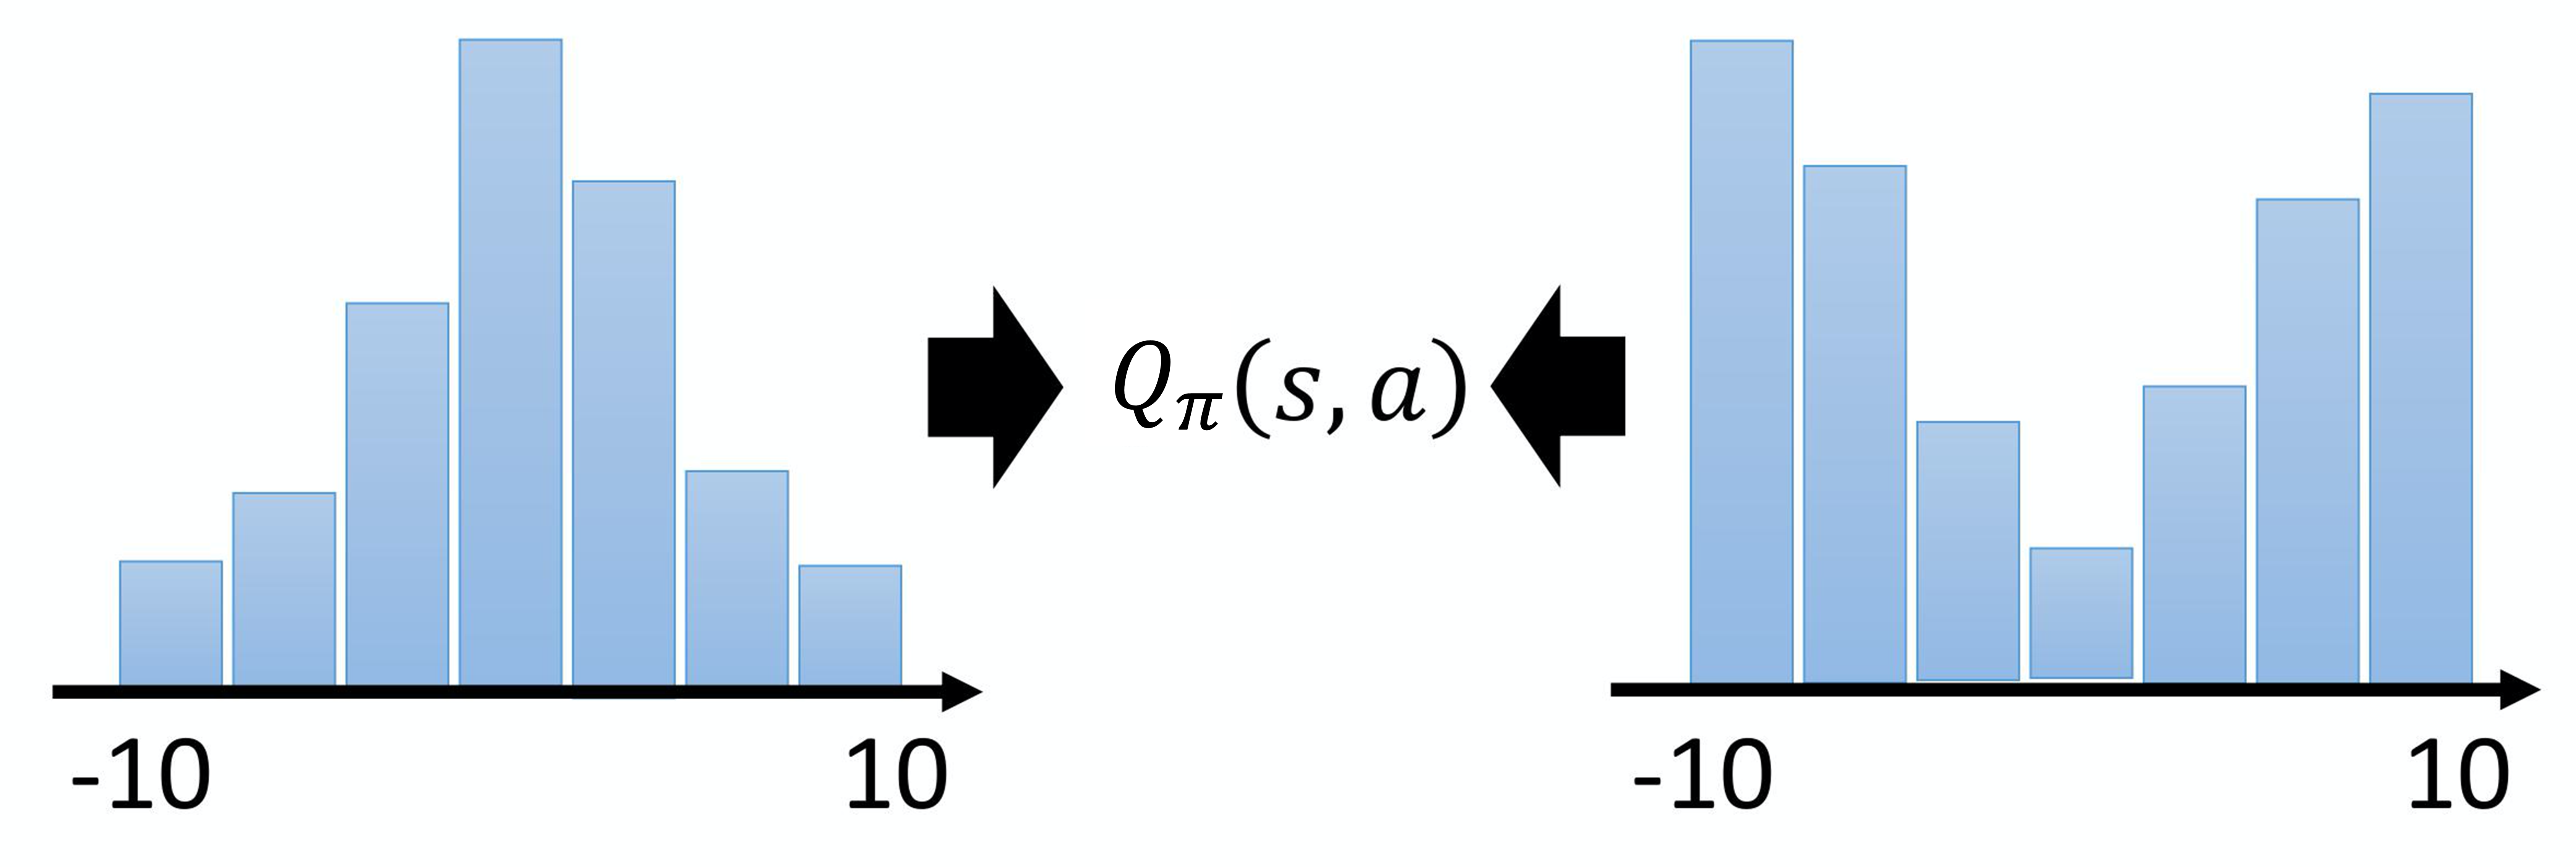
\includegraphics[width=0.5\linewidth]{res/ch7/7.11}
    \caption{奖励分布}
    \label{fig:fig7.11}
\end{figure}

分布式Q函数是对分布(distribution)建模,怎么做呢?
如\figref{fig:7.12a} 所示,
在原来的Q函数里面,假设我们只能采取 $a_1$、$a_2$、$a_3$ 这3 个动作,我们输入一个状态,输出 3 个值。这3 个值分别代表 3 个动作的 Q 值,但是这些 Q 值是一个分布的期望值。所以分布式Q函数就是直接输出分布。
实际上的做法如\figref{fig:7.12b} 所示,
假设分布的值就分布在某一个范围里面,比如 $-$10 \~{} 10,把 $-$10 \~{} 10 拆成一个一个的长条。例如,每一个动作的奖励空间拆成 5 个长条。假设奖励空间可以拆成 5 个长条,Q函数的输出就是要预测我们在某一个状态采取某一个动作得到的奖励,其落在某一个长条里面的概率。
所以绿色长条概率的和应该是 1,其高度代表在某一个状态采取某一个动作的时候,它落在某一个长条内的概率。绿色的代表动作 $a_1$,红色的代表动作 $a_2$,蓝色的代表动作 $a_3$。所以我们就可以用Q函数去估计 $a_1$ 的分布、$a_2$ 的分布、$a_3$ 的分布。实际上在做测试的时候,我们选平均值最大的动作执行。

\begin{figure}[htb]
    \centering
    \subfloat[一个拥有3个输出的网络]{
        \label{fig:7.12a}
        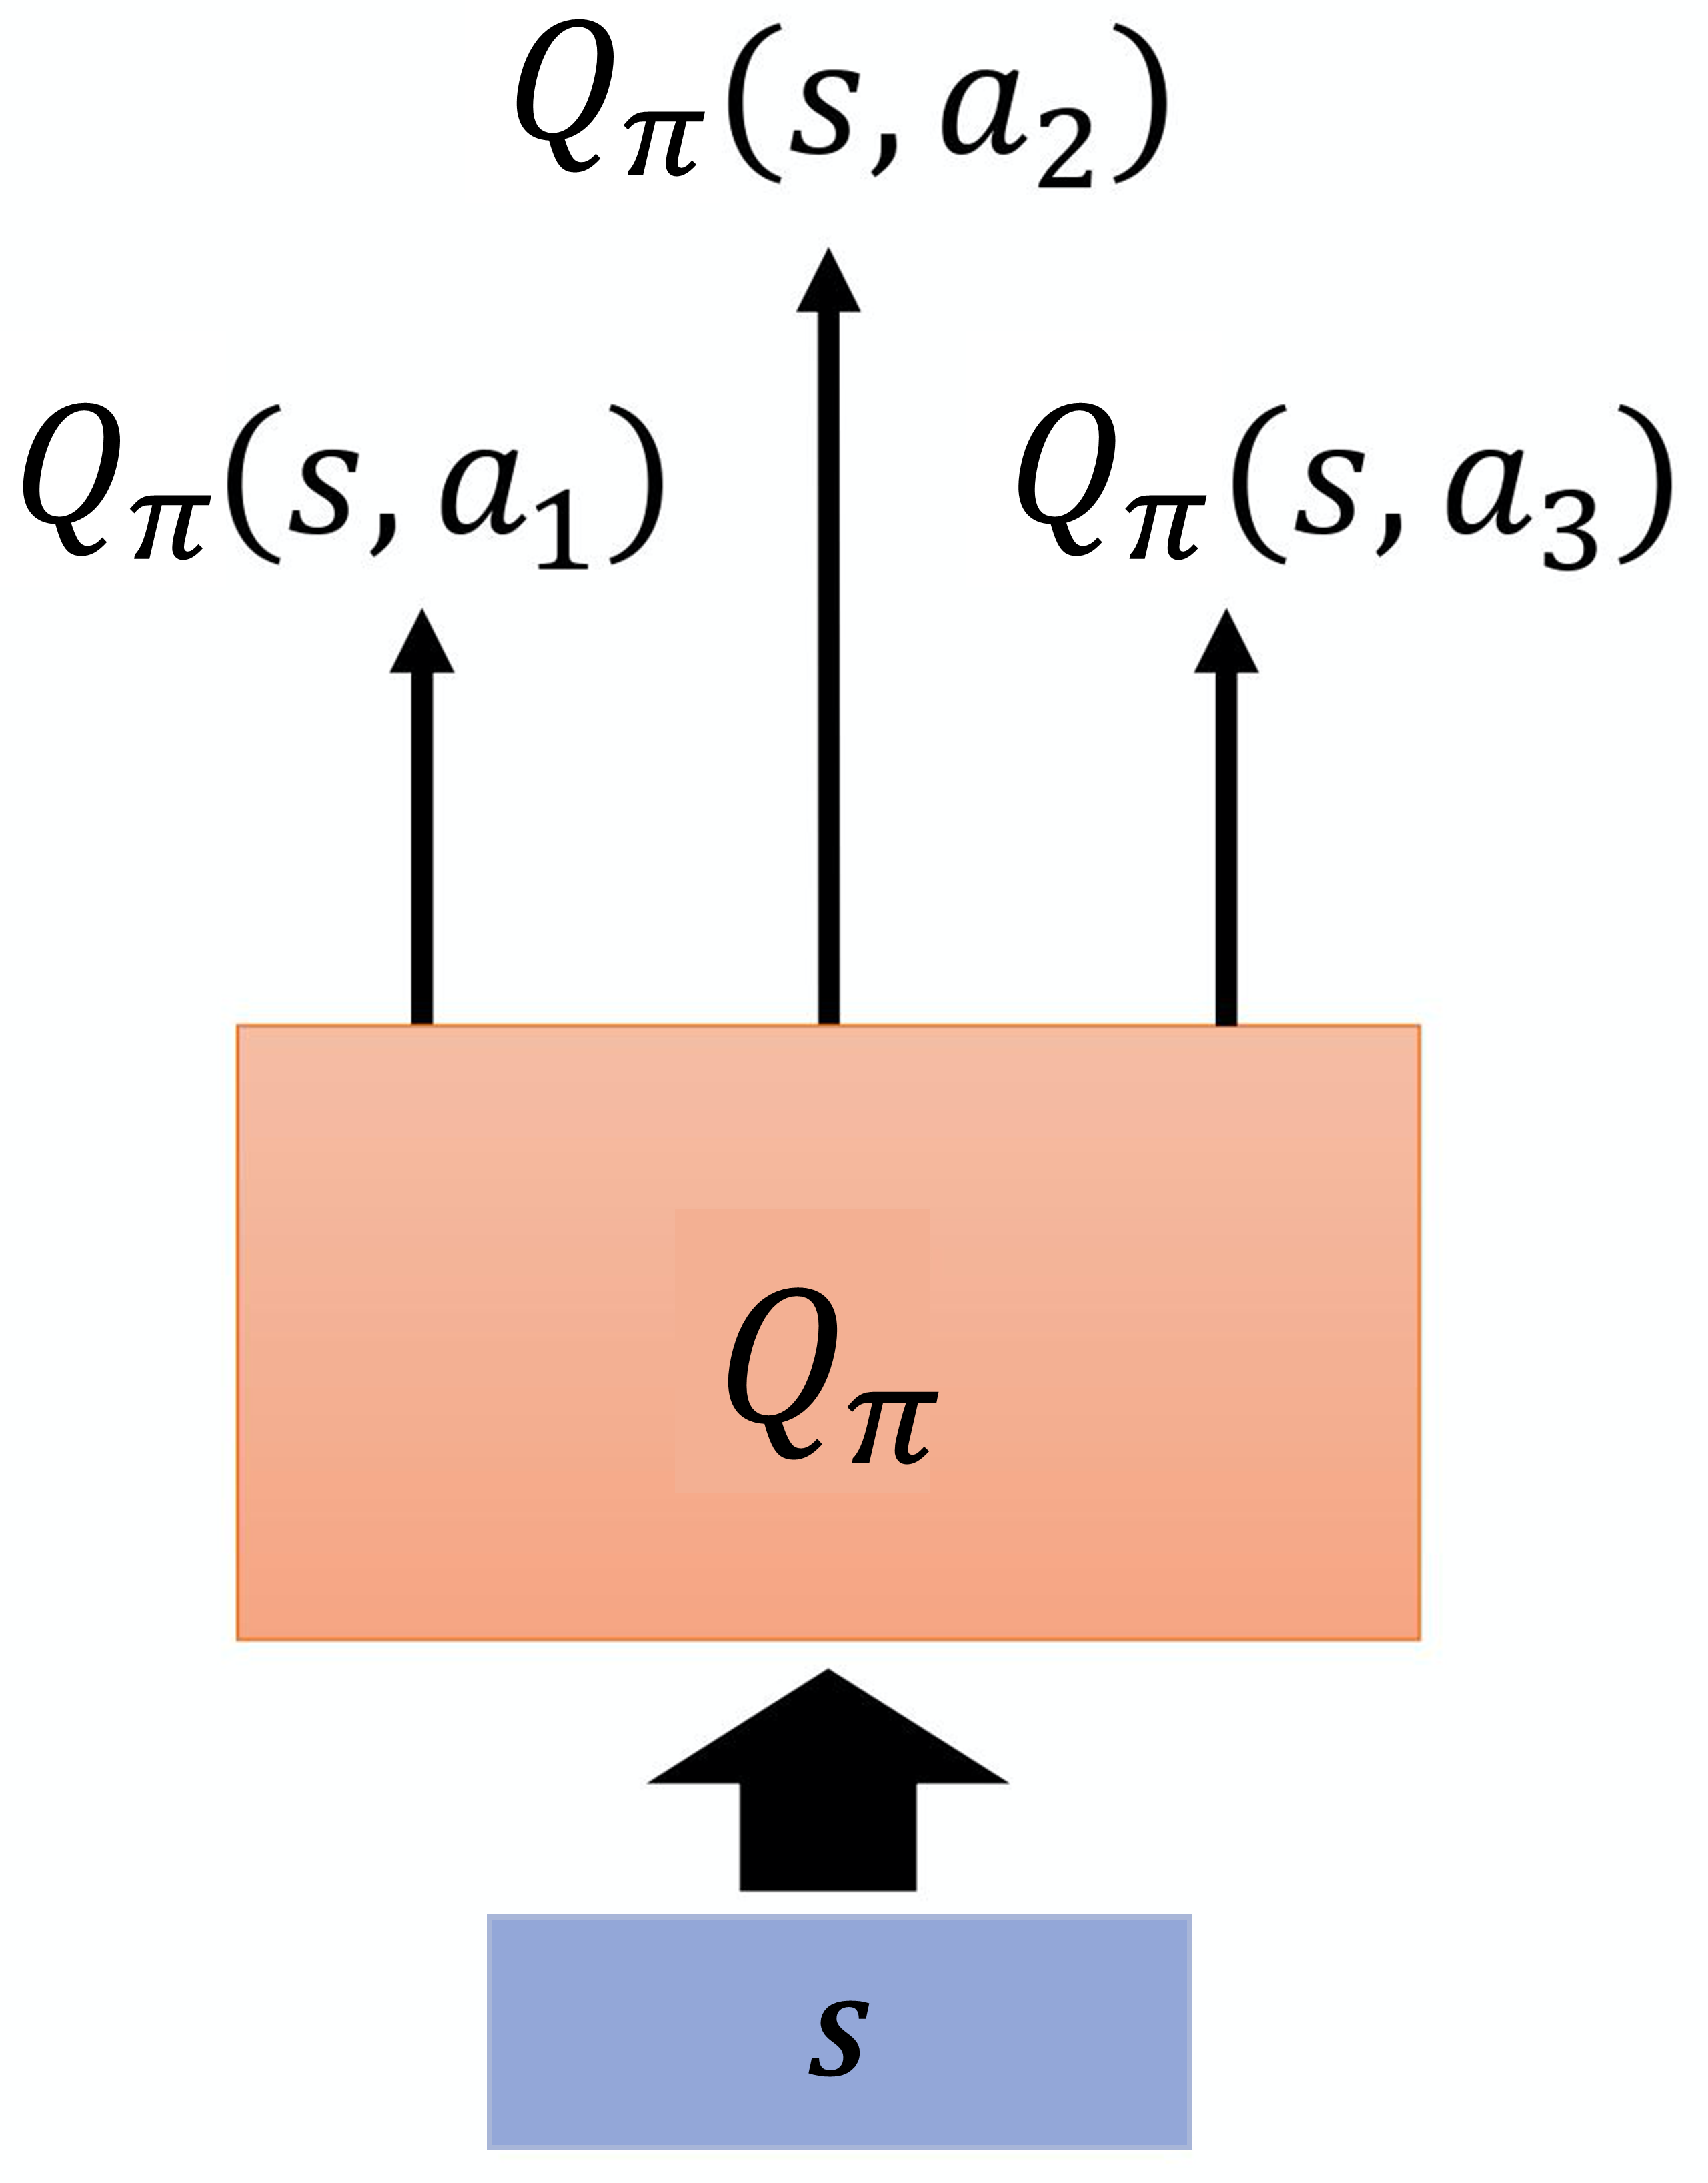
\includegraphics[width=0.3\linewidth]{res/ch7/7.12a}
    }
    \subfloat[一个拥有15个输出的网络(每一个动作对应5个长条)]{
        \label{fig:7.12b}
        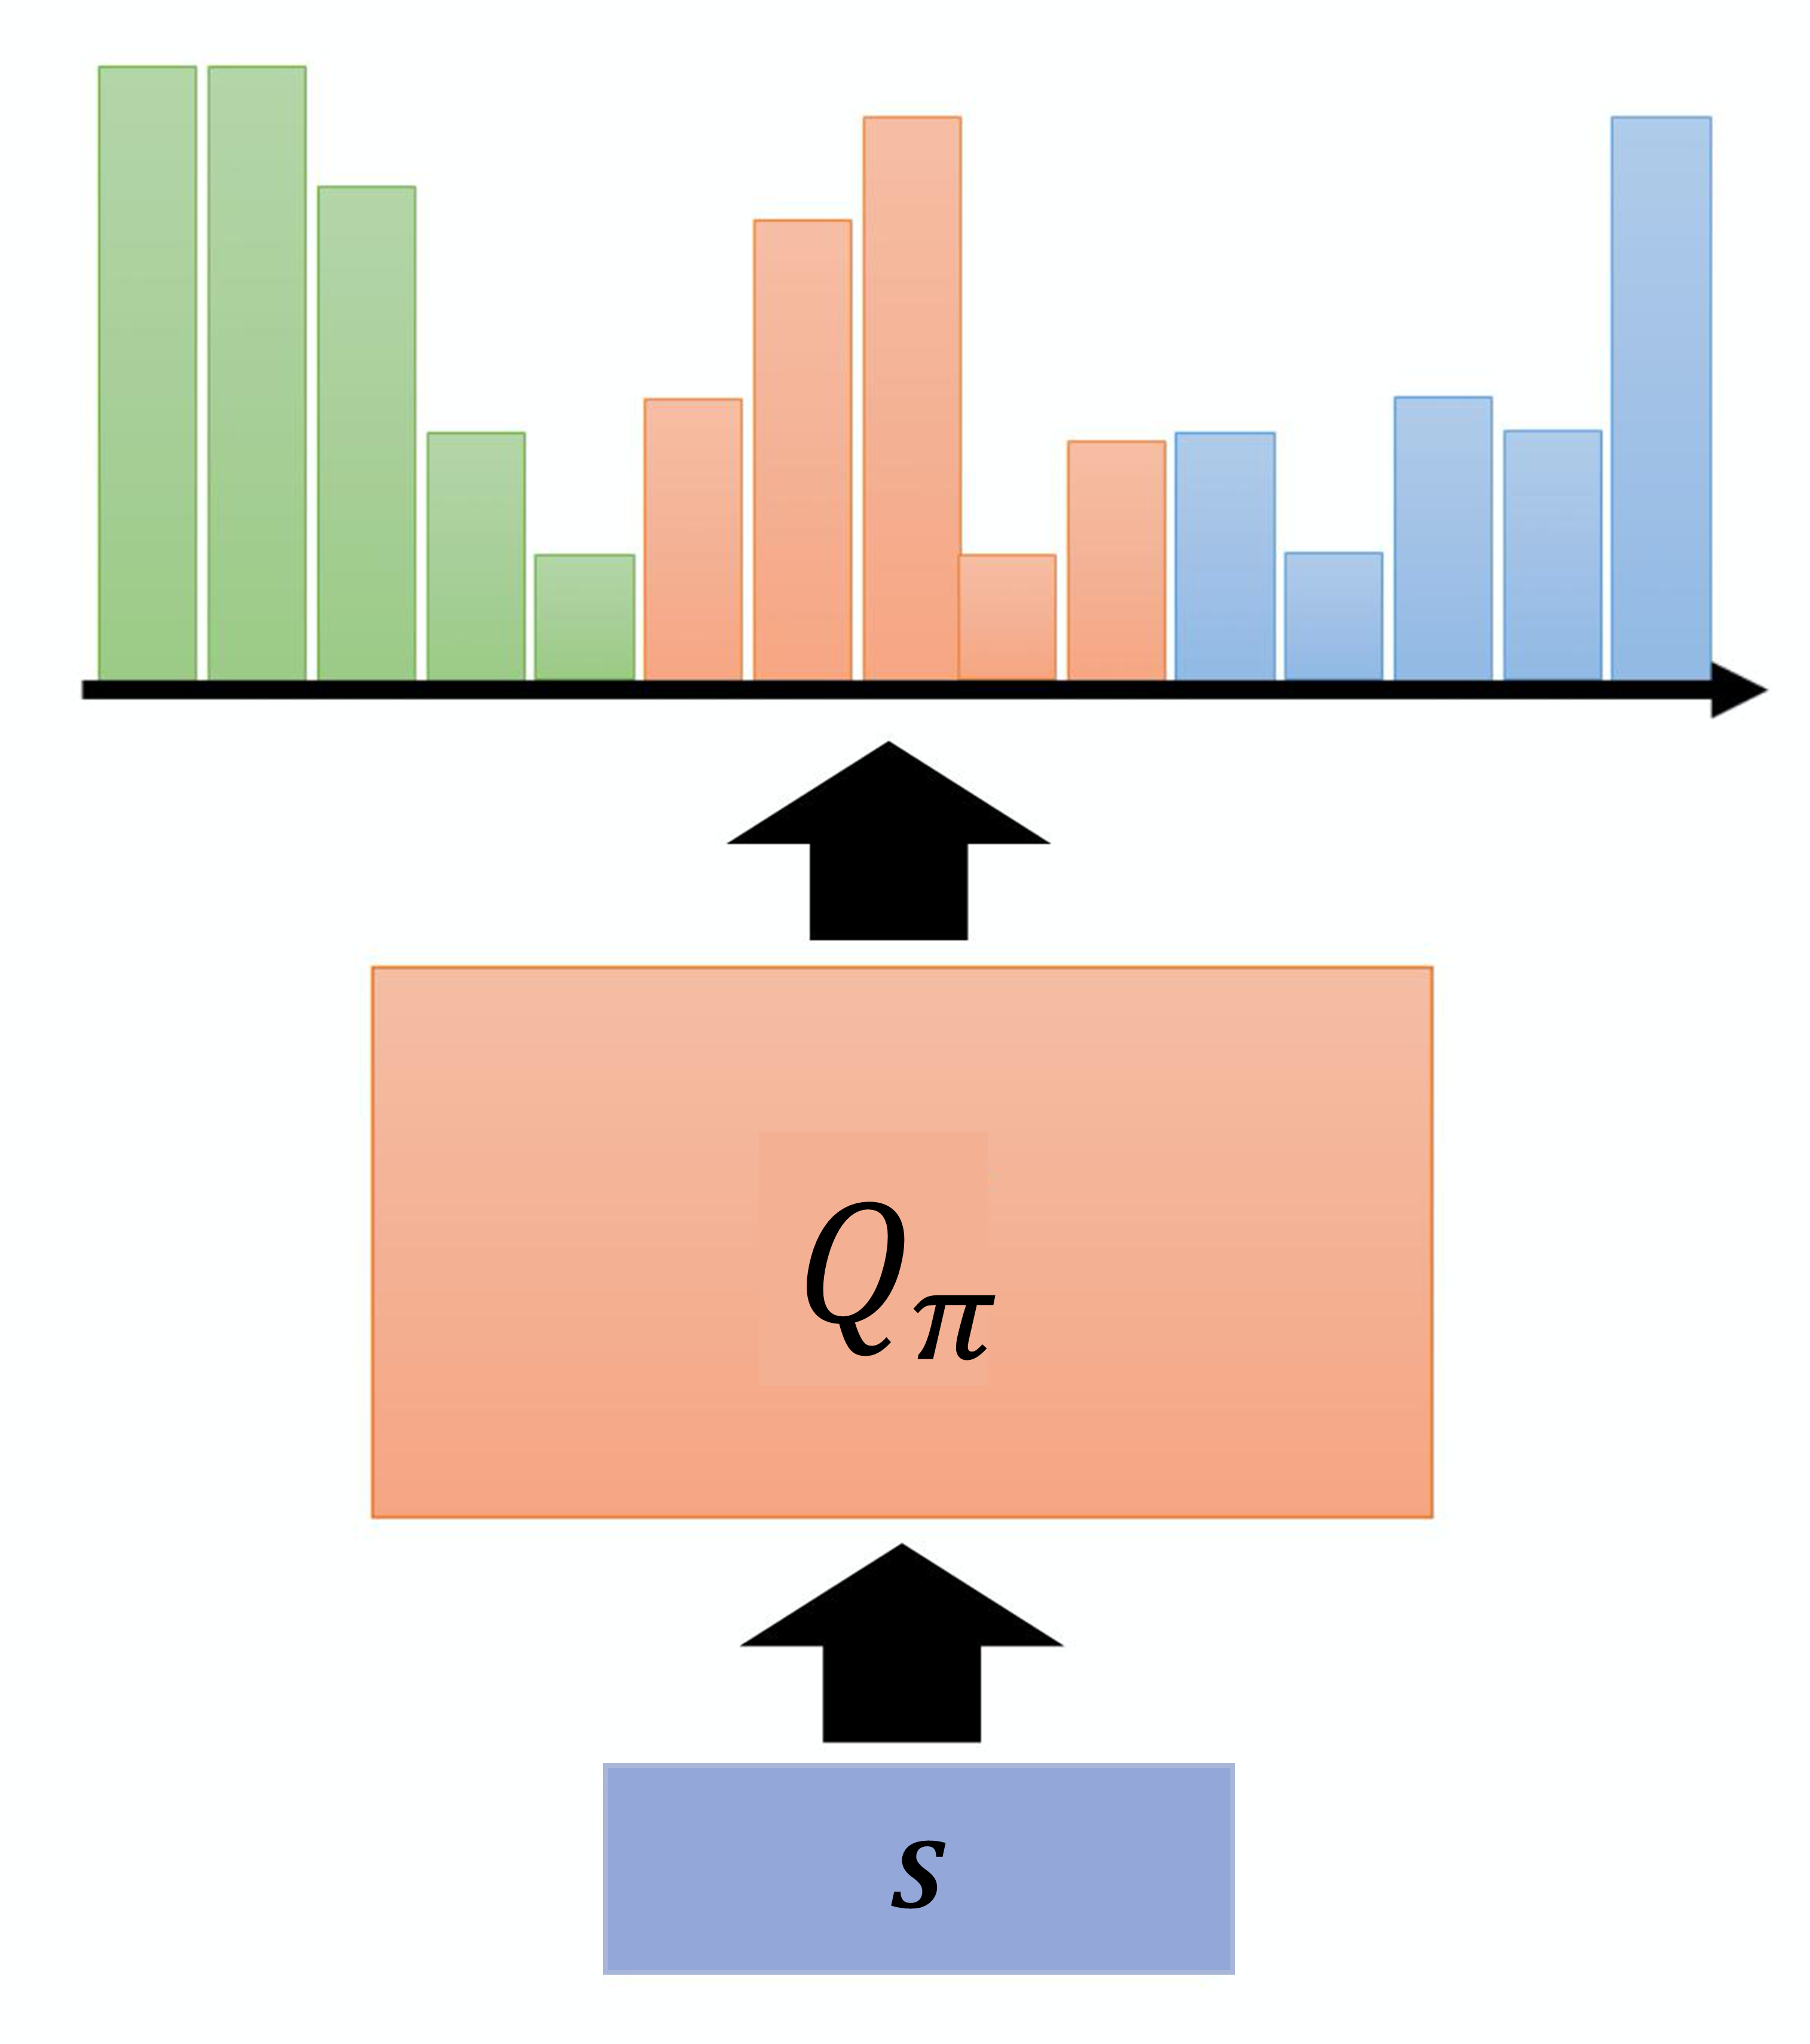
\includegraphics[width=0.3\linewidth]{res/ch7/7.12b}
    }
    \caption{分布式Q函数}
    \label{fig:distributional_q_2}
\end{figure}

除了选平均值最大的动作以外,我们还可以对分布建模。例如,我们可以考虑动作的分布,如果分布方差很大,这代表采取这个动作虽然平均而言很不错,但也许风险很高,我们可以训练一个网络来规避风险。在两个动作平均值都差不多的情况下,也许可以选一个风险比较小的动作来执行,这就是分布式Q函数的好处。

\subsection{彩虹} 

最后一个技巧称为\kw{彩虹(rainbow)},
如\figref{fig:rainbow} 所示,假设每个方法有一种自己的颜色(如果每一个单一颜色的线代表只用某一个方法),把所有的颜色组合起来,就变成“彩虹”,我们把原来的深度Q网络也算作一种方法,故有 7 种颜色。
横轴代表训练过程的帧数,纵轴代表玩十几个雅达利小游戏的平均分数的和,但它取的是分数的中位数。为什么是取中位数而不是直接取平均呢?
因为不同小游戏的分数差距很大,如果取平均,某几个游戏可能会控制结果,因此我们取中位数。
如果我们使用的是一般的深度Q网络(灰色的线),深度Q网络的性能不是很好。噪声深度Q网络(noisy DQN)比DQN的性能好很多。紫色的线代表 DDQN,DDQN 还挺有效的。优先级经验回放的双深度Q网络(prioritized DDQN)、竞争双深度Q网络(dueling DDQN)和分布式深度Q网络(distributional DQN)性能也挺高的。
\kw{异步优势演员-评论员(asynchronous advantage actor-critic,A3C)}是演员-评论员的方法,A3C算法又被译作异步优势动作评价算法,我们会在第九章详细介绍异步优势演员-评论员算法。
单纯的异步优势演员-评论员算法看起来是比深度Q网络强的。\figref{fig:rainbow} 中没有多步方法,这是因为异步优势演员-评论员算法本身内部就有多步方法,所以实现异步优势演员-评论员算法就等同于实现多步方法,我们可以把 异步优势演员-评论员算法的结果看成多步方法的结果。这些方法本身之间是没有冲突的,我们把全部方法都用上就变成了七彩的方法,即彩虹方法,彩虹方法的性能很好。

\begin{figure}[htb]
    \centering
    \includegraphics[width=0.4\linewidth]{res/ch7/7.13}
    \caption{彩虹方法\upcite{rainbow_paper}}
    \label{fig:rainbow}
\end{figure}

我们把所有的方法加在一起,模型的表现会提高很多,但会不会有些方法其实是没有用的呢?我们可以去掉其中一种方法来判断这个方法是否有用。如\figref{fig:rainbow_2} 所示,虚线就是彩虹方法去掉某一种方法以后的结果,黄色的虚线去掉多步方法后“掉”很多。彩虹是彩色的实线,去掉多步方法会“掉下来”,去掉优先级经验回放后会“掉下来”,去掉分布也会“掉下来”。
这边有一个有趣的地方,在开始的时候,分布训练的方法与其他方法速度差不多。但是我们去掉分布训练方法的时候,训练不会变慢,但是性能(performance)最后会收敛在比较差的地方。我们去掉噪声网络后性能也差一点儿,去掉竞争深度 Q 网络后性能也差一点儿,去掉双深度 Q 网络却没什么差别。所以我们把全部方法组合在一起的时候,去掉双深度 Q 网络是影响比较小的。当我们使用分布式深度Q网络的时候,本质上就不会高估奖励。我们是为了避免高估奖励才加了DDQN。如果我们使用了分布式深度Q网络,就可能不会有高估的结果,多数的情况是低估奖励的,所以变成DDQN没有用。

为什么分布式深度Q网络不会高估奖励奖励,反而会低估奖励呢?因为分布式深度Q网络输出的是一个分布的范围,输出的范围不可能是无限的,我们一定会设一个限制, 比如最大输出范围就是从 $-$10 \~{} 10。假设得到的奖励超过 10,比如 100 怎么办?我们就当作没看到这件事,所以奖励很极端的值、很大的值是会被丢弃的,用分布式深度Q网络的时候,我们不会高估奖励,反而会低估奖励。

\begin{figure}[htb]
    \centering
    \includegraphics[width=0.4\linewidth]{res/ch7/7.14}
    \caption{彩虹:去掉其中一种方法\upcite{rainbow_paper}}
    \label{fig:rainbow_2}
\end{figure}

\subsection{使用深度 Q 网络解决推车杆问题}

在学习本节之前,可以先回顾一下之前的项目实战,即使用Q学习解决悬崖寻路问题。本节将具体实现深度 Q 网络算法来解决推车杆问题,对应的模拟环境为 OpenAI Gym 中的 CartPole-v0 ,我们同样先对该环境做一个简要说明。

\subsubsection{CartPole-v0 简介} 

CartPole-v0是一个经典的入门环境,如\figref{fig:cliffwalking} 所示,它通过向左(动作 = 0)或向右(动作 = 1)推动推车来实现推车杆的平衡。每次实施一个动作后,如果杆能够继续保持平衡,就会得到一个 $+1$ 的奖励,否则杆将无法保持平衡而导致游戏结束。理论上最优算法情况下,推车杆是能够一直保证平衡的,但是如果每回合无限制地进行下去,会影响到算法的训练,所以环境一般设置每回合的最大步数为200。另外 Gym 官方也推出了另外一版的推车杆环境,名为CartPole-v1,相比 v0 版本,v1每回合最大步数为500,其他基本不变,可以说是 v0 的难度升级版。

\begin{figure}[htb]
    \centering
    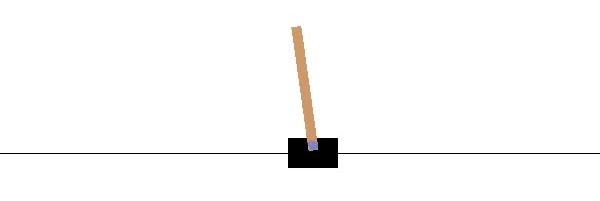
\includegraphics[width=0.6\linewidth]{res/ch7/assets/poster.jpg}
    \caption{CartPole-v0 环境}
    \label{fig:cliffwalking}
\end{figure}

我们来看看这个环境的一些参数,执行以下代码:

\begin{lstlisting}[style=Python]
    import gym
    env = gym.make('CartPole-v0')  # 建立环境
    env.seed(1) # 随机种子
    n_states = env.observation_space.shape[0] # 状态数
    n_actions = env.action_space.n # 动作数
    print(f"状态数:{n_states},动作数:{n_actions}")
\end{lstlisting}

可以得到结果:

\begin{lstlisting}[language=sh,basicstyle=\zihao{-5}\ttfamily] 
    状态数:4,动作数:2
\end{lstlisting}

该环境的状态数是4个,分别为车的位置、车的速度、杆的角度以及杆顶部的速度;动作数为2个,并且是离散的向左或者向右。

我们也可以直接重置或者初始化环境看看初始状态,代码如下:

\begin{lstlisting}[style=Python]
    state = env.reset() # 初始化环境
    print(f"初始状态:{state}")
\end{lstlisting}

结果为:

\begin{lstlisting}[language=sh,basicstyle=\zihao{-5}\ttfamily] 
    初始状态:[0.03073904  0.00145001 -0.03088818 -0.03131252]
\end{lstlisting}

\subsubsection{深度Q网络基本接口} 

介绍完环境之后,我们沿用接口的概念,通过分析伪代码来实现深度 Q 网络的基本训练模式。其实所有的强化学习算法都遵循同一个训练思路,执行动作,环境反馈,然后智能体更新,只是不同算法需要的一些要素不同,我们需要分析出这些要素,比如建立什么网络需要什么模块,以进一步完善算法。

我们现在常用的 深度Q网络 伪代码如\figref{fig:dqn} 所示。

\begin{figure}[htb]
    \centering
    
\includegraphics[width=0.75\linewidth]{res/ch7/assets/dqn.png}
    \caption{深度 Q 网络算法伪代码}
    \label{fig:dqn}
\end{figure}

用代码实现如下:

\begin{lstlisting}[style=Python]
    rewards = [] # 记录奖励
    ma_rewards = []  # 记录滑动平均奖励
    for i_ep in range(cfg.train_eps):
        state = env.reset() # 初始化环境
        done = False
        ep_reward = 0
        while True:
            action = agent.choose_action(state)
            next_state, reward, done, _ = env.step(action)
            ep_reward += reward
            agent.memory.push(state, action, reward, next_state, done)
            state = next_state
            agent.update()
            if done:
                break
        if (i_ep+1) % cfg.target_update == 0:
            agent.target_net.load_state_dict(agent.policy_net.state_dict())
        if (i_ep+1)%10 == 0:
            print('回合:{}/{}, 奖励:{}'.format(i_ep+1, cfg.train_eps, ep_reward))
        rewards.append(ep_reward)
        if ma_rewards:
            ma_rewards.append(0.9*ma_rewards[-1]+0.1*ep_reward)
        else:
            ma_rewards.append(ep_reward)
\end{lstlisting}

可以看到, 深度 Q 网络的训练模式其实和大多强化学习算法是一样的思路,但与传统的 Q 学习算法相比, 深度 Q 网络使用神经网络来代替之前的Q表格从而存储更多的信息,且由于使用了神经网络,因此我们一般需要利用随机梯度下降来优化 Q 值的预测。此外深度 Q 网络多了回放缓冲区,并且使用两个网络,即目标网络和当前网络。

\subsubsection{回放缓冲区} 

从伪代码中可以看出,回放缓冲区的功能有两个:一个是将每一步采集的经验(包括状态、动作、奖励、下一时刻的状态)存储到缓冲区中,并且缓冲区具有一定的容量(capacity);另一个是在更新策略的时候需要随机采样小批量的经验进行优化。因此我们可以定义一个 ReplayBuffer 类,包括 push() 和 sample() 两个函数,用于存储和采样。

\begin{lstlisting}[style=Python]
    import random
    class ReplayBuffer:
        def __init__(self, capacity):
            self.capacity = capacity # 回放缓冲区的容量
            self.buffer = [] # 缓冲区
            self.position = 0 
        
        def push(self, state, action, reward, next_state, done):
            ''' 缓冲区是一个队列,容量超出时删除开始存入的经验
            '''
            if len(self.buffer) < self.capacity:
                self.buffer.append(None)
            self.buffer[self.position] = (state, action, reward, next_state, done)
            self.position = (self.position + 1) % self.capacity 
        
        def sample(self, batch_size):
            batch = random.sample(self.buffer, batch_size) # 随机采小批量经验
            state, action, reward, next_state, done =  zip(*batch) # 解压成状态、动作等
            return state, action, reward, next_state, done
        def __len__(self):
            ''' 返回当前存储的量
            '''
            return len(self.buffer)
\end{lstlisting}

\subsubsection{ Q 网络} 

在深度 Q 网络中我们使用神经网络替代原有的Q表格,从而能够存储更多的Q值,实现更为高级的策略以便用于复杂的环境。这里我们用的是一个三层的感知机或者称之为连接网络:

\begin{lstlisting}[style=Python]
    class MLP(nn.Module):
        def __init__(self, input_dim,output_dim,hidden_dim=128):
            """ 初始化Q网络,为全连接神经网络
                input_dim: 输入的特征数即环境的状态数
                output_dim: 输出的动作维度
            """
            super(MLP, self).__init__()
            self.fc1 = nn.Linear(input_dim, hidden_dim) # 输入层
            self.fc2 = nn.Linear(hidden_dim,hidden_dim) # 隐藏层
            self.fc3 = nn.Linear(hidden_dim, output_dim) # 输出层
            
        def forward(self, x):
            # 各层对应的激活函数
            x = F.relu(self.fc1(x)) 
            x = F.relu(self.fc2(x))
            return self.fc3(x)
\end{lstlisting}

学过深度学习的读者应该对全连接神经网络十分熟悉。在强化学习中,网络的输入一般是状态,输出则是一个动作,假如总共有两个动作,那么这里的动作维度就是2,可能的输出就是0或1,一般我们用 ReLU 作为激活函数。根据实际需要也可以改变神经网络的模型结构等等,比如若我们使用图像作为输入,则可以使用卷积神经网络(convolutional neural network,CNN)。

\subsubsection{深度Q网络算法}

与前面的项目实战一样,深度 Q 算法一般也包括选择动作和更新策略两个函数,首先我们看选择动作:

\begin{lstlisting}[style=Python]
    def choose_action(self, state):
        '''选择动作
        '''
        self.frame_idx += 1
        if random.random() > self.epsilon(self.frame_idx):
            with torch.no_grad():
                state = torch.tensor([state], device=self.device, dtype=torch.float32)
                q_values = self.policy_net(state)
                action = q_values.max(1)[1].item() # 选择Q值最大的动作
        else:
            action = random.randrange(self.action_dim)
\end{lstlisting}

可以看到跟深度 Q 网络算法与 Q 学习算法其实是一样的,都是用的$\varepsilon$-贪心策略,只是深度 Q 网络算法我们需要通过 PyTorch 或者 TensorFlow 工具来处理相应的数据。

而深度 Q 网络算法更新策略的步骤稍微复杂一点儿,主要包括三个部分:随机采样、计算期望 Q 值和梯度下降,如下:

\begin{lstlisting}[style=Python]
    def update(self):
        if len(self.memory) < self.batch_size: # 当memory中不满足一个批量时,不更新策略
            return
        # 从回放缓冲区中随机采样一个批量的经验
        state_batch, action_batch, reward_batch, next_state_batch, done_batch = self.memory.sample(
            self.batch_size)
        # 转为张量
        state_batch = torch.tensor(state_batch, device=self.device, dtype=torch.float)
        action_batch = torch.tensor(action_batch, device=self.device).unsqueeze(1)  
        reward_batch = torch.tensor(reward_batch, device=self.device, dtype=torch.float)  
        next_state_batch = torch.tensor(next_state_batch, device=self.device, dtype=torch.float)
        done_batch = torch.tensor(np.float32(done_batch), device=self.device)
        
        q_values = self.policy_net(state_batch).gather(dim=1, index=action_batch) # 计算当前状态(s_t,a)对应的Q(s_t,a)
        next_q_values = self.target_net(next_state_batch).max(1)[0].detach() # 计算下一时刻的状态(s_t_,a)对应的Q值
        # 计算期望的Q值,对于终止状态,此时done_batch[0]=1, 对应的expected_q_values等于reward
        expected_q_values = reward_batch + self.gamma * next_q_values * (1-done_batch)
        loss = nn.MSELoss()(q_values, expected_q_values.unsqueeze(1))  # 计算均方根损失
        # 优化更新模型
        self.optimizer.zero_grad()  
        loss.backward()
        for param in self.policy_net.parameters():  # clip防止梯度爆炸
            param.grad.data.clamp_(-1, 1)
        self.optimizer.step() 
\end{lstlisting}

\subsubsection{结果分析}

实现代码之后,我们先来看看深度 Q 网络算法的训练效果,如\figref{fig:train_rewards_curve_cn-1689150.png} 所示。

\begin{figure}[htb]
    \centering
    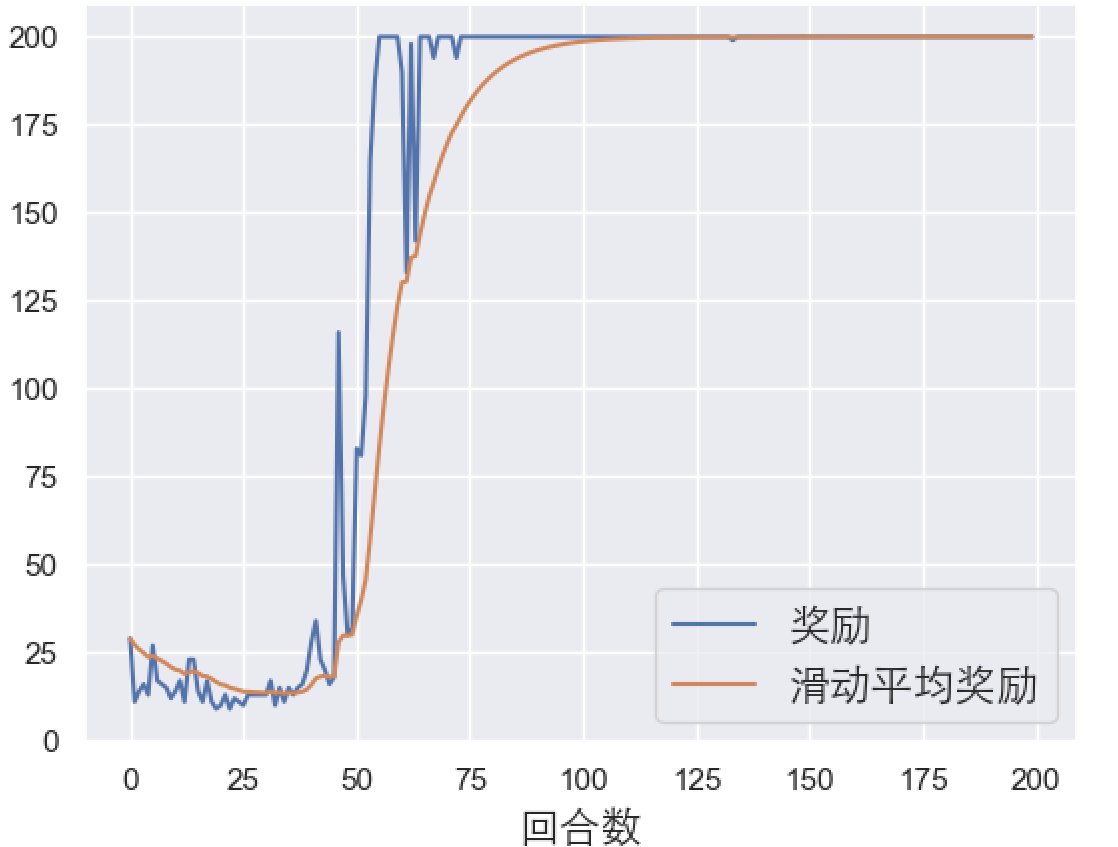
\includegraphics[width=0.6\linewidth]{res/ch7/assets/train_rewards_curve_cn-1689150.png}
    \caption{CartPole-v0 环境下深度 Q 网络算法的训练曲线}
    \label{fig:train_rewards_curve_cn-1689150.png}
\end{figure}

从\figref{fig:train_rewards_curve_cn-1689150.png} 中可以看出,算法其实已经在 60 回合左右达到收敛,最后一直维持在最佳奖励 200 左右,可能会有轻微的波动,这是因为我们在收敛的情况下依然保持了一定的探索率,即 epsilon\_end=0.01 。现在我们可以载入模型看看测试的效果,如\figref{fig:eval_rewards_curve_cn-1689282.png} 所示。

\begin{figure}[htb]
    \centering
    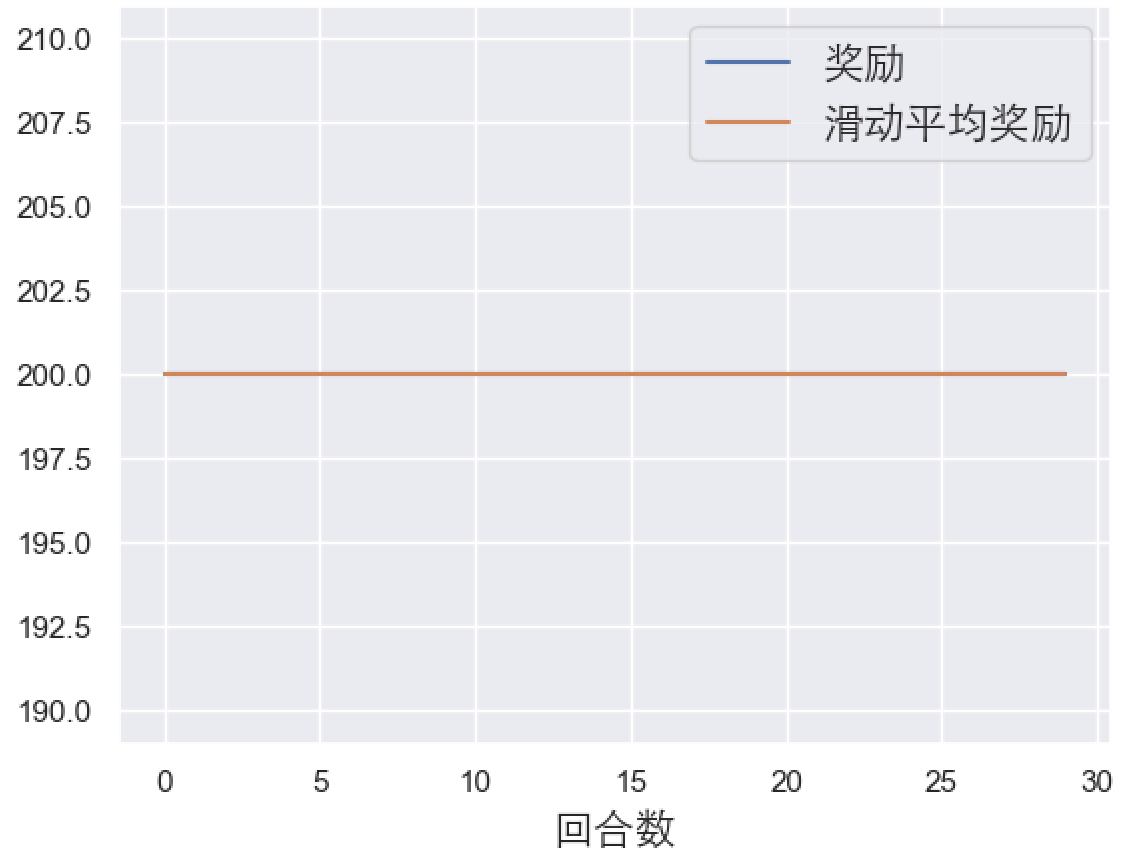
\includegraphics[width=0.6\linewidth]{res/ch7/assets/eval_rewards_curve_cn-1689282.png}
    \caption{CartPole-v0 环境下深度 Q 网络算法的测试曲线}
    \label{fig:eval_rewards_curve_cn-1689282.png}
\end{figure}

我们测试了 30 个回合,每个回合奖励都保持在 200 左右,说明我们的模型学习得不错!

\subsection{关键词}

双深度Q网络(double DQN):在双深度Q网络中存在两个Q网络,第一个Q网络决定哪一个动作的Q值最大,从而决定对应的动作。另一方面,Q值是用 $Q'$ 计算得到的,这样就可以避免过度估计的问题。具体地,假设我们有两个Q函数并且第一个Q函数高估了它现在执行的动作 $a$ 的值,这没关系,只要第二个Q函数 $Q'$ 没有高估动作 $a$ 的值,那么计算得到的就还是正常的值。

竞争深度Q网络(dueling DQN):将原来的深度Q网络的计算过程分为两步。第一步计算一个与输入有关的标量 $\mathrm{V(s)}$;第二步计算一个向量 $\mathrm{A(s,a)}$ 对应每一个动作。最后的网络将两步的结果相加,得到我们最终需要的Q值。用一个公式表示就是 $\mathrm{Q(s,a)=V(s)+A(s,a)}$ 。另外,竞争深度Q网络,使用状态价值函数与动作价值函数来评估Q值。

优先级经验回放(prioritized experience replay,PER):这个方法是为了解决我们在第6章中提出的经验回放方法的不足而提出的。我们在使用经验回放时,均匀地取出回放缓冲区(reply buffer)中的采样数据,这里并没有考虑数据间的权重大小。但是我们应该将那些训练效果不好的数据对应的权重加大,即其应该有更大的概率被采样到。综上,优先级经验回放不仅改变了被采样数据的分布,还改变了训练过程。

噪声网络(noisy net):其在每一个回合开始的时候,即智能体要和环境交互的时候,在原来的Q函数的每一个参数上加上一个高斯噪声(Gaussian noise),把原来的Q函数变成 $\tilde{Q}$ ,即噪声Q函数。同样,我们把每一个网络的权重等参数都加上一个高斯噪声,就得到一个新的网络 $\tilde{Q}$ 。我们会使用这个新的网络与环境交互直到结束。

分布式Q函数(distributional Q-function):对深度Q网络进行模型分布,将最终网络的输出的每一类别的动作再进行分布操作。

彩虹(rainbow):将第6、7章7个技巧综合起来的方法,7个技巧分别是——深度Q网络、双深度Q网络、优先级经验回放的双深度Q网络、竞争深度Q网络、异步优势演员-评论员算法(A3C)、分布式Q函数、噪声网络,进而考察每一个技巧的贡献度或者与环境的交互是否是正反馈的。


\subsection{习题}

\kw{7-1} 为什么传统的深度Q网络的效果并不好?可以参考其公式 $Q(s_t ,a_t)=r_t+\max_{a}Q(s_{t+1},a)$ 来描述。

\kw{7-2} 在传统的深度Q网络中,我们应该怎么解决目标值太大的问题呢?

\kw{7-3} 请问双深度Q网络中所谓的 $Q$ 与 $Q'$ 两个网络的功能是什么?

\kw{7-4} 如何理解竞争深度Q网络的模型变化带来的好处?

\kw{7-5} 使用蒙特卡洛和时序差分平衡方法的优劣分别有哪些?


\subsection{面试题}

\kw{7-1} 友善的面试官:深度Q网络都有哪些变种?引入状态奖励的是哪种?

\kw{7-2} 友善的面试官:请简述双深度Q网络原理。

\kw{7-3} 友善的面试官:请问竞争深度Q网络模型有什么优势呢?

\bibliographystyle{gbt7714-numerical}
\bibliography{ref.bib}




    % 
\section{ DDPG 算法}
\subsection{ DPG 算法}
\subsection{ DDPG 算法}
\subsection{实战:DDPG算法}

简单引出最大熵强化学习

\subsection{关键词}
\subsection{习题}
\subsection{面试题}
\subsection{本章小结}
    % \section{演员-评论员算法}
在REINFORCE算法中,每次需要根据一个策略采集一条完整的轨迹,并计算这条轨迹上的回报。这种采样方式的方差比较大,学习效率也比较低。我们可以借鉴时序差分学习的思想,使用动态规划方法来提高采样效率,即从状态 $s$ 开始的总回报可以通过当前动作的即时奖励 $r(s,a,s')$ 和下一个状态 $s'$ 的值函数来近似估计。

\kw{演员-评论员算法}是一种结合\kw{策略梯度}和\kw{时序差分学习}的强化学习方法,其中,
演员是指策略函数 $\pi_{\theta}(a|s)$,即学习一个策略以得到尽可能高的回报。
评论员是指价值函数 $V_{\pi}(s)$,对当前策略的值函数进行估计,即评估演员的好坏。
借助于价值函数,演员-评论员算法可以进行单步参数更新,不需要等到回合结束才进行更新。
在演员-评论员算法里面,最知名的算法就是异步优势演员-评论员算法。
如果我们去掉异步,则为\kw{优势演员-评论员(advantage actor-critic,A2C)算法}。A2C算法又被译作优势演员-评论员算法。
如果我们加了异步,变成异步优势演员-评论员算法。

\subsection{策略梯度回顾} 
我们复习一下策略梯度,在更新策略参数 $\theta$ 的时候,我们可以通过
\begin{equation}
  \label{eq:policy_gradient}
  \nabla \bar{R}_{\theta} \approx \frac{1}{N} \sum_{n=1}^{N} \sum_{t=1}^{T_{n}}\left(\sum_{t^{\prime}=t}^{T_{n}} \gamma^{t^{\prime}-t} r_{t^{\prime}}^{n}-b\right) \nabla \log p_{\theta}\left(a_{t}^{n} \mid s_{t}^{n}\right)
\end{equation}
来计算梯度。
\eqref{eq:policy_gradient} 表示我们首先通过智能体与环境的交互,可以计算出在某一个状态 $s$ 采取某一个动作 $a$ 的概率  $p_{\theta}(a_t|s_t)$。接下来,我们计算在某一个状态 $s$ 采取某一个动作 $a$ 之后直到游戏结束的累积奖励。$\sum_{t^{\prime}=t}^{T_{n}} \gamma^{t^{\prime}-t} r_{t^{\prime}}^{n}$ 表示我们把从时间 $t$ 到时间 $T$ 的奖励相加,并且在前面乘一个折扣因子,通常将折扣因子设置为 0.9 或 0.99等数值,与此同时也会减去一个基线值 $b$,减去值 $b$ 的目的是希望括号里面这一项是有正有负的。如果括号里面这一项是正的,我们就要增大在这个状态采取这个动作的概率;如果括号里面是负的,我们就要减小在这个状态采取这个动作的概率。

我们使用 $G$ 表示累积奖励,$G$ 是非常不稳定的。因为交互的过程本身具有随机性,所以在某一个状态 $s$ 采取某一个动作 $a$ 时计算得到的累积奖励,每次结果都是不同的,因此 $G$ 是一个随机变量。对于同样的状态 $s$ 和同样的动作 $a$,$G$ 可能有一个固定的分布。但由于我们采取采样的方式,因此我们在某一个状态 $s$ 采取某一个动作 $a$ 一直到游戏结束,统计一共得到了多少的奖励,我们就把它当作 $G$。

如\figref{fig:fig9.1} 所示,如果我们把 $G$ 想成一个随机变量,实际上是在对 $G$ 做采样,用这些采样的结果去更新参数。但实际上在某一个状态 $s$ 采取某一个动作 $a$,接下来会发生什么事,其本身是有随机性的。虽然说有一个固定的分布,但其方差可能会非常大。智能体在同一个状态采取同一个动作时,最后得到的结果可能会是很不一样的。
当然,假设我们在每次更新参数之前,都可以采样足够多次,那当然就没有以上的问题了。但我们每次做策略梯度,每次更新参数之前都要做一些采样时,采样的次数是不可能太多的,我们只能够做非常少量的采样。如果我们正好采样到差的结果,比如采样到 $G = 100$、采样到 $G = -10$,显然结果会是很差的。

\begin{figure}[hbt]
  \centering
  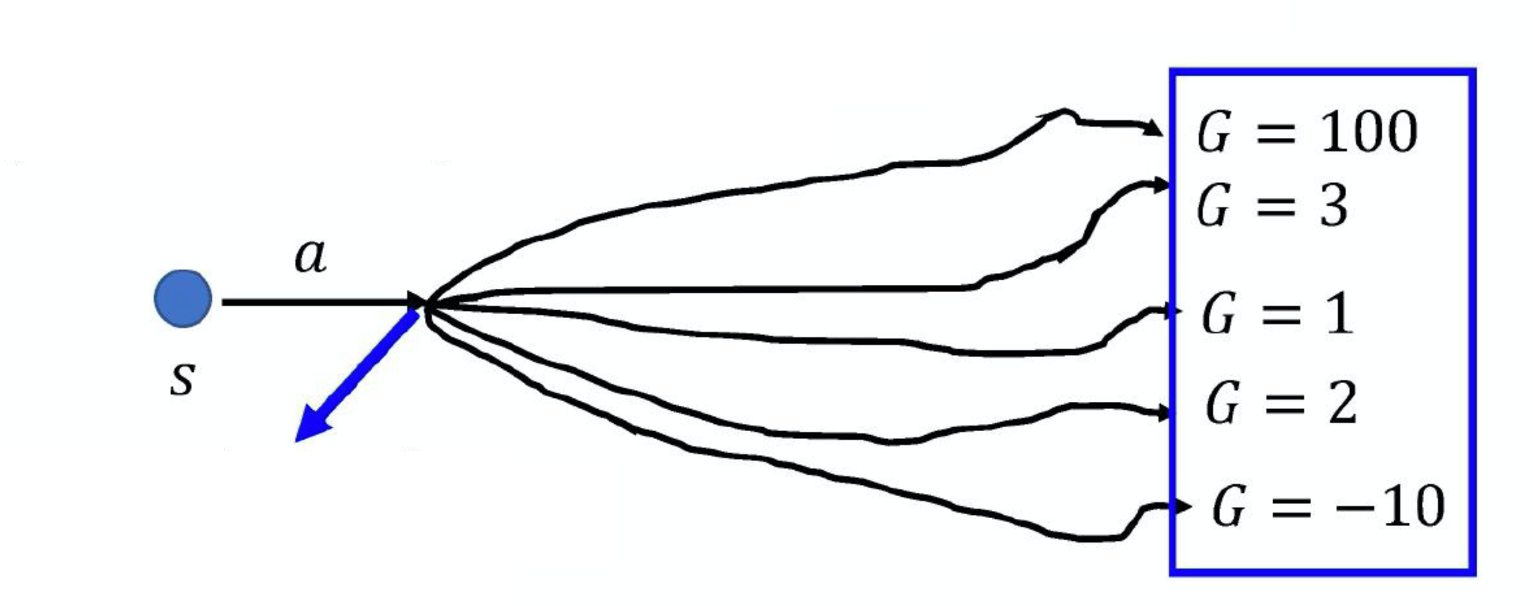
\includegraphics[width=0.4\linewidth]{res/ch9/9.1}
  \caption{策略梯度回顾}
  \label{fig:fig9.1}
\end{figure}

\subsection{深度Q网络回顾}

Q:我们能不能让整个训练过程变得稳定,能不能直接估测随机变量 $G$ 的期望值?

A:我们直接用一个网络去估测在状态 $s$ 采取动作 $a$ 时 $G$ 的期望值。如果这样是可行的,那么在随后的训练中我们就用期望值代替采样的值,这样就会让训练变得更加稳定。

Q:怎么使用期望值代替采样的值呢?

A:这里就需要引入基于价值的(value-based)的方法。基于价值的方法就是 深度Q网络 。深度Q网络 有两种函数,有两种评论员。
如\figref{fig:fig9.2} 所示,
  第一种评论员是 $V_{\pi}(s)$。即假设演员的策略是 $\pi$,使用 $\pi$ 与环境交互,当智能体看到状态 $s$ 时,接下来累积奖励的期望值是多少。
  第二种评论员是 $Q_{\pi}(s,a)$。$Q_{\pi}(s,a)$ 把 $s$ 与 $a$ 当作输入,它表示在状态 $s$ 采取动作 $a$,接下来用策略 $\pi$ 与环境交互,累积奖励的期望值是多少。
  $V_{\pi}$ 接收输入 $s$,输出一个标量。
  $Q_{\pi}$ 接收输入 $s$,它会给每一个 $a$ 都分配一个 Q值。
%   我们可以用时序差分或蒙特卡洛来估计。两者的区别是,用时序差分比较稳定,用 蒙特卡洛 比较精确。


\begin{figure}[hbt]
  \centering
  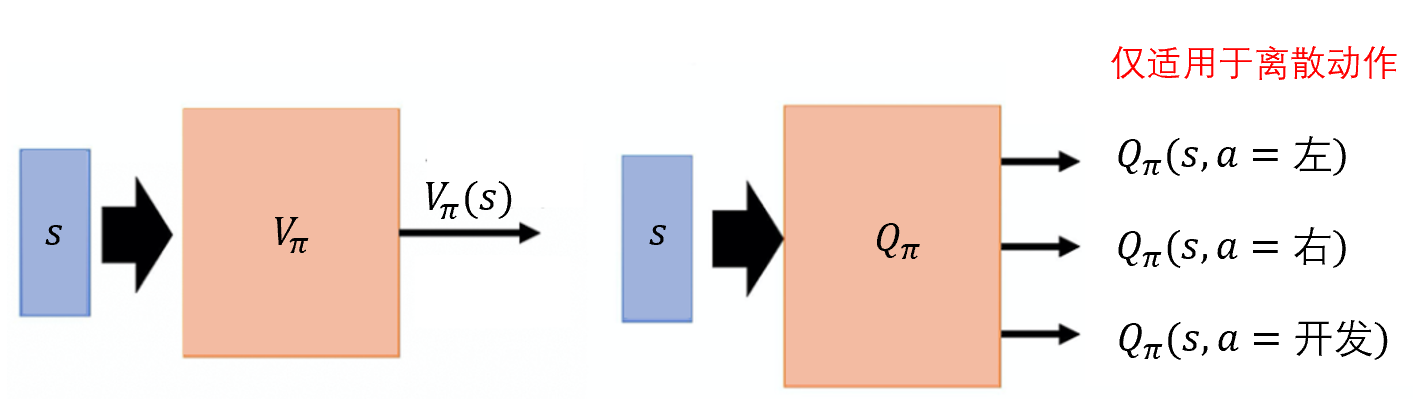
\includegraphics[width=0.7\linewidth]{res/ch9/9.2}
  \caption{深度Q网络}
  \label{fig:fig9.2}
\end{figure}

\subsection{优势演员-评论员算法}
如\figref{fig:fig9.3} 所示,
随机变量 $G$ 的期望值正好就是 Q 值,即
\begin{equation}
  \label{eq:}
  \mathbb{E}\left[G_{t}^{n}\right]=Q_{\pi_{\theta}} \left(s_{t}^{n}, a_{t}^{n}\right)
\end{equation}
此也为 Q 函数的定义。Q函数的定义就是在某一个状态 $s$,采取某一个动作 $a$,假设策略是 $\pi$ 的情况下所能得到的累积奖励的期望值,即 $G$ 的期望值。累积奖励的期望值就是 $G$ 的期望值。
所以假设用 $\mathbb{E}\left[G_{t}^{n}\right]$ 来代表 $\sum_{t^{\prime}=t}^{T_{n}} \gamma^{t^{\prime}-t} r_{t^{\prime}}^{n}$ 这一项,把Q函数套在这里就结束了,我们就可以把演员与评论员这两个方法结合起来。

有不同的方法表示基线,一个常见的方法是用价值函数 $V_{\pi_{\theta}}\left(s_{t}^{n}\right)$ 来表示基线。价值函数的定义为,假设策略是 $\pi$,其在某个状态 $s$ 一直与环境交互直到游戏结束,期望奖励有多大。 $V_{\pi_{\theta}}\left(s_{t}^{n}\right)$ 没有涉及动作,$Q_{\pi_{\theta}}\left(s_{t}^{n}, a_{t}^{n}\right)$ 涉及动作。
$V_{\pi_{\theta}}\left(s_{t}^{n}\right)$ 是 $Q_{\pi_{\theta}}\left(s_{t}^{n}, a_{t}^{n}\right)$ 的期望值, $Q_{\pi_{\theta}}\left(s_{t}^{n}, a_{t}^{n}\right)-V_{\pi_{\theta}}\left(s_{t}^{n}\right)$ 会有正有负,所以 $\sum_{t^{\prime}=t}^{T_{n}} \gamma^{t^{\prime}-t} r_{t^{\prime}}^{n}-b$ 这一项就会有正有负。
所以我们就把策略梯度里面 $\sum_{t^{\prime}=t}^{T_{n}} \gamma^{t^{\prime}-t} r_{t^{\prime}}^{n}-b$ 这一项换成了优势函数$A^{\theta}\left(s^{n}_{t}, a^{n}_{t}\right)$,即 $Q_{\pi_{\theta}}\left(s_{t}^{n}, a_{t}^{n}\right)-V_{\pi_{\theta}}\left(s_{t}^{n}\right)$。因此该算法称为优势演员-评论员算法。
\begin{figure}[hbt]
  \centering
  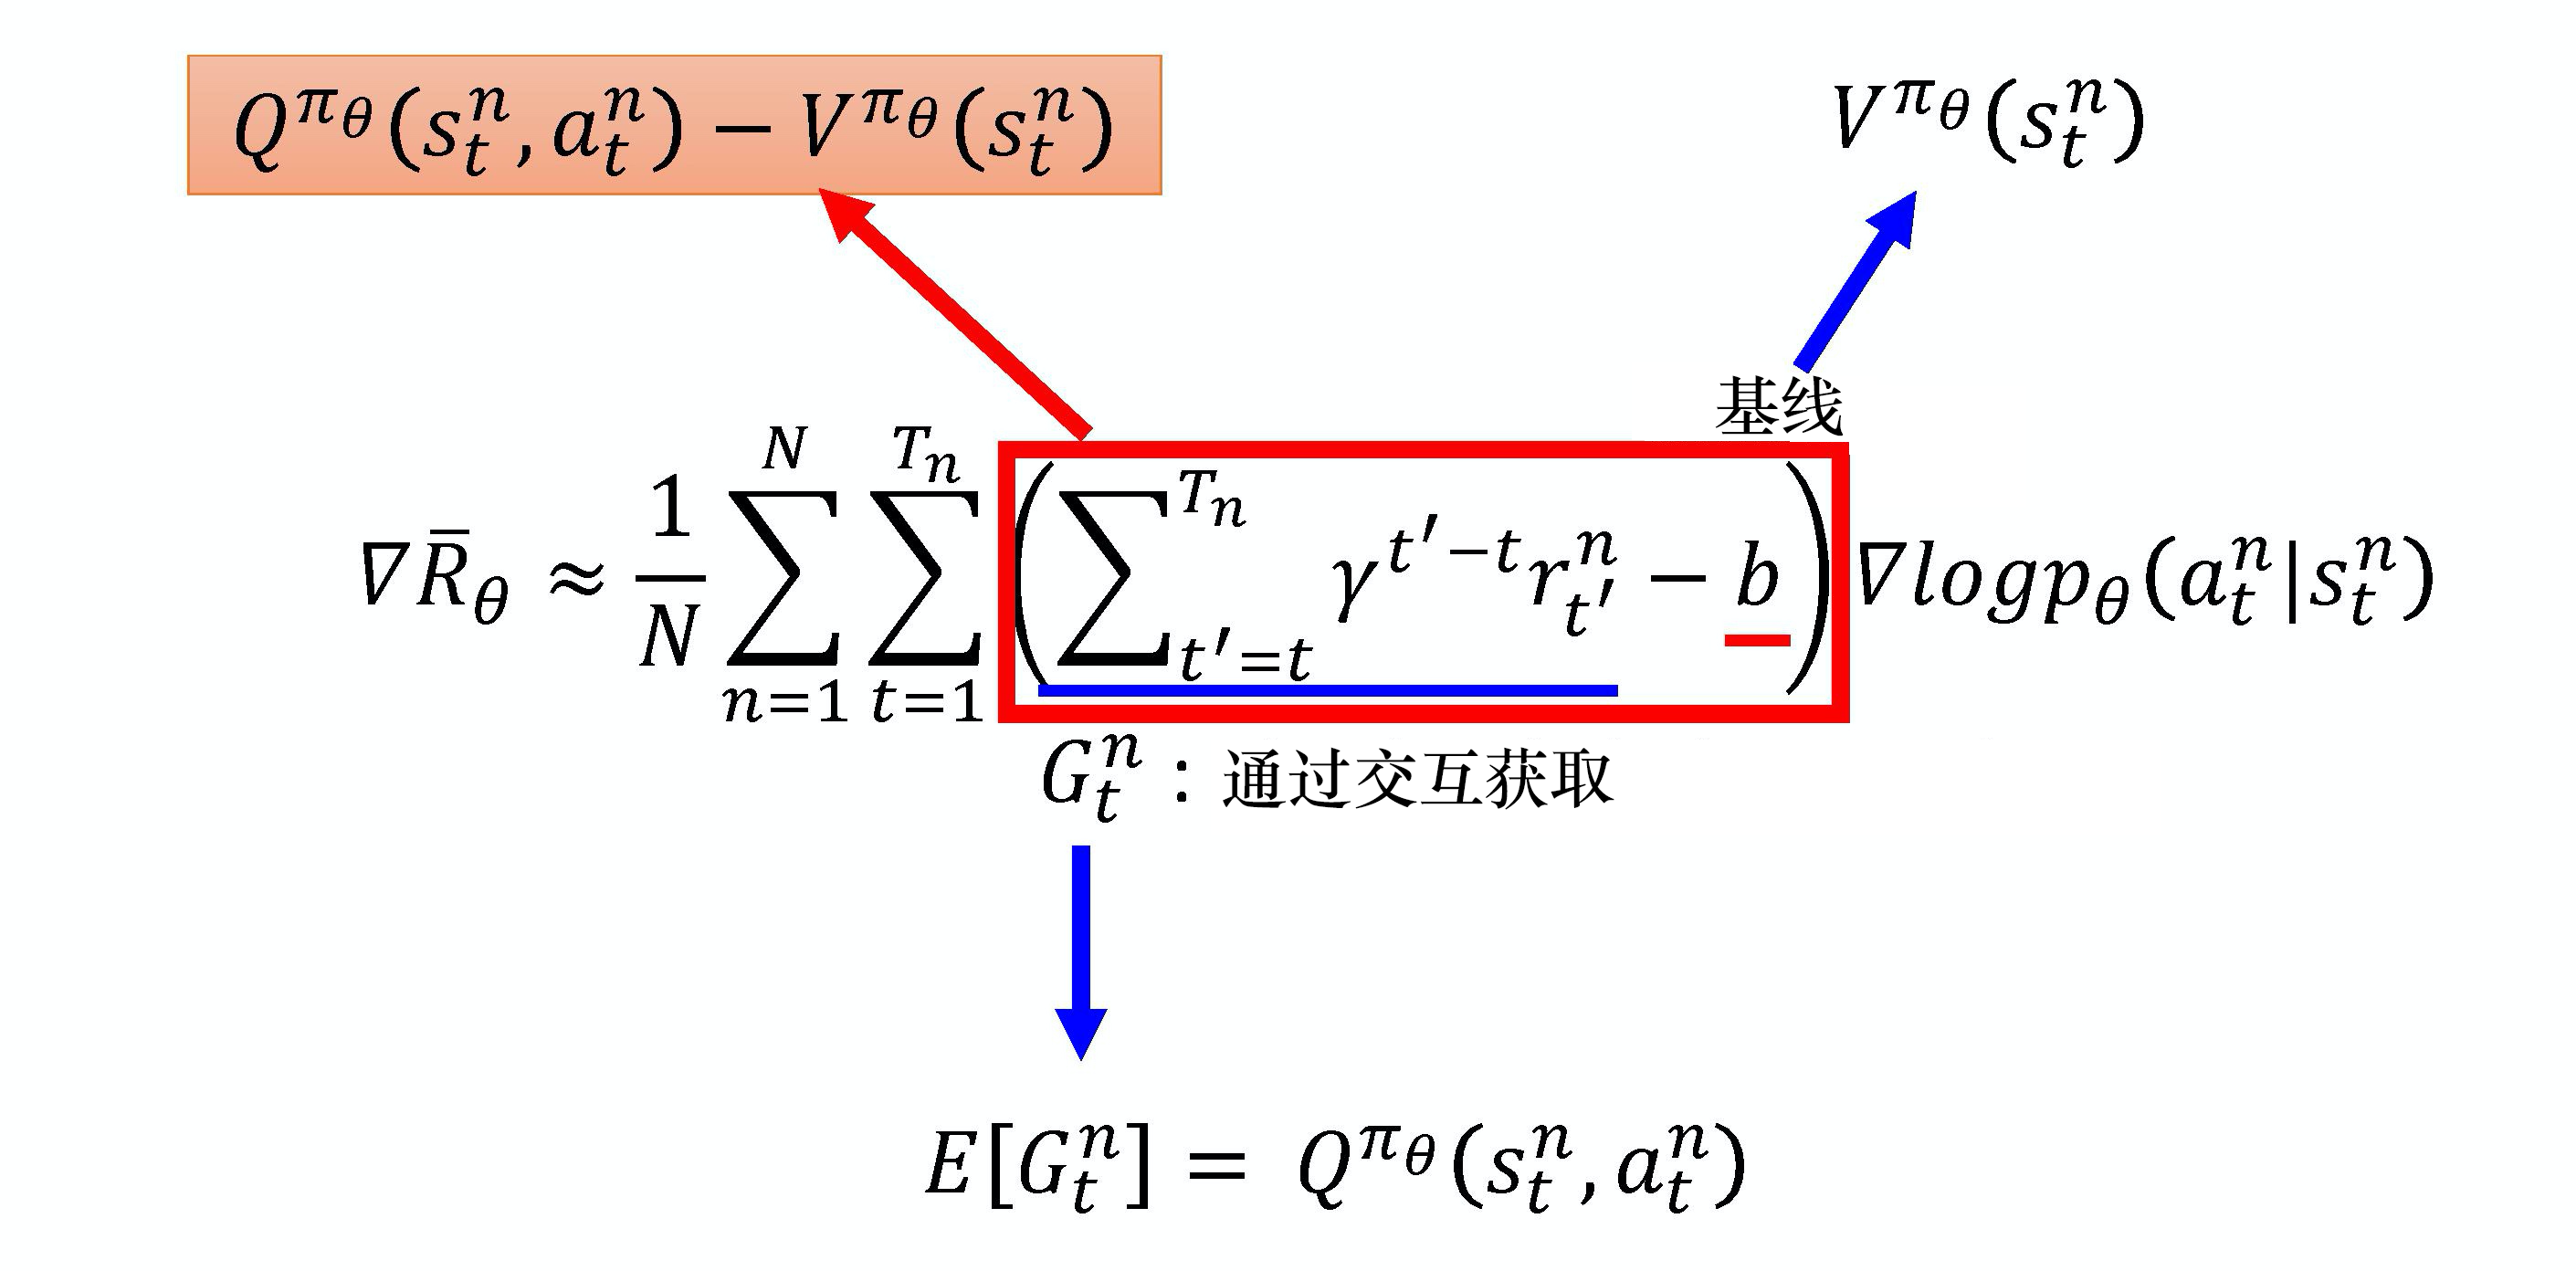
\includegraphics[width=0.5\linewidth]{res/ch9/9.3}
  \caption{优势演员-评论员算法}
  \label{fig:fig9.3}
\end{figure}

如果我们这么实现,有一个缺点,即我们需要估计两个网络------Q网络和 V网络,估计不准的风险就变成原来的两倍。所以我们何不只估计一个网络呢?
事实上,在演员-评论员算法中,我们可以只估计网络 V,并利用 $V$ 的值来表示 $Q$ 的值,$Q_{\pi}\left(s_{t}^{n}, a_{t}^{n}\right)$ 可以写成 $ r_{t}^{n}+V_{\pi}\left(s_{t+1}^{n}\right)$ 的期望值,即
\begin{equation}
  \label{eq:}
  Q_{\pi}\left(s_{t}^{n}, a_{t}^{n}\right)=\mathbb{E}\left[r_{t}^{n}+V_{\pi}\left(s_{t+1}^{n}\right)\right]
\end{equation}

在状态 $s$ 采取动作 $a$,我们会得到奖励 $r$,进入状态 $s_{t+1}$。但是我们会得到什么样的奖励 $r$,进入什么样的状态 $s_{t+1}$,这件事本身是有随机性的。所以要把$r_{t}^{n}+V_{\pi}\left(s_{t+1}^{n}\right)$取期望值才会等于Q函数的值。但我们现在把取期望值去掉,即
\begin{equation}
  \label{eq:}
  Q_{\pi}\left(s_{t}^{n}, a_{t}^{n}\right)=r_{t}^{n}+V_{\pi}\left(s_{t+1}^{n}\right)
\end{equation}

我们就可以把Q函数的值用 $r_t^n + V_{\pi}\left(s_{t+1}^{n}\right)$ 取代,可得
\begin{equation}
  \label{eq:}
  r_{t}^{n}+V_{\pi}\left(s_{t+1}^{n}\right)-V_{\pi}\left(s_{t}^{n}\right)
\end{equation}

把取期望值去掉的好处就是我们不需要估计 $Q$ 了,只需要估计 $V$。但与此同时我们会引入一个随机的参数 $r$。$r$ 是有随机性的,它是一个随机变量,但是 $r$ 相较于累积奖励 $G$ 是一个较小的值,因为它是某一个步骤得到的奖励,而 $G$ 是所有未来会得到的奖励的总和,$G$ 的方差比较大。$r$ 虽然也有一些方差,但它的方差比 $G$ 的要小。所以把原来方差比较大的 $G$ 换成方差比较小的 $r$ 也是合理的。

Q:为什么我们可以直接把取期望值去掉?

A:原始的异步优势演员-评论员算法的论文尝试了各种方法,最后发现这个方法最好。当然有人可能会有疑问,说不定估计 $Q$ 和 $V$ 也可以估计得很好,但实际做实验的时候,最后结果就是这个方法最好,所以后来大家都使用了这个方法。

优势演员-评论员算法的流程如\figref{fig:fig9.5} 所示,我们有一个 $\pi$,有个初始的演员与环境交互,先收集资料。在策略梯度方法里收集资料以后,就来更新策略。但是在演员-评论员算法里面,我们不是直接使用那些资料来更新策略。我们先用这些资料去估计价值函数,可以用 时序差分方法 或 蒙特卡洛方法 来估计价值函数。接下来,我们再基于价值函数,使用\eqref{eq:update_pi} 更新 $\pi$。
\begin{equation}
  \label{eq:update_pi}
  \nabla \bar{R}_{\theta} \approx \frac{1}{N} \sum_{n=1}^{N} \sum_{t=1}^{T_{n}}\left(r_{t}^{n}+V_{\pi}\left(s_{t+1}^{n}\right)-V_{\pi}\left(s_{t}^{n}\right)\right) \nabla \log p_{\theta}\left(a_{t}^{n} \mid s_{t}^{n}\right)
\end{equation}
有了新的 $\pi$ 以后,再与环境交互,收集新的资料,去估计价值函数。再用新的价值函数更新策略,更新演员。
整个优势演员-评论员算法就是这么运作的。

\begin{figure}[h]
  \centering
  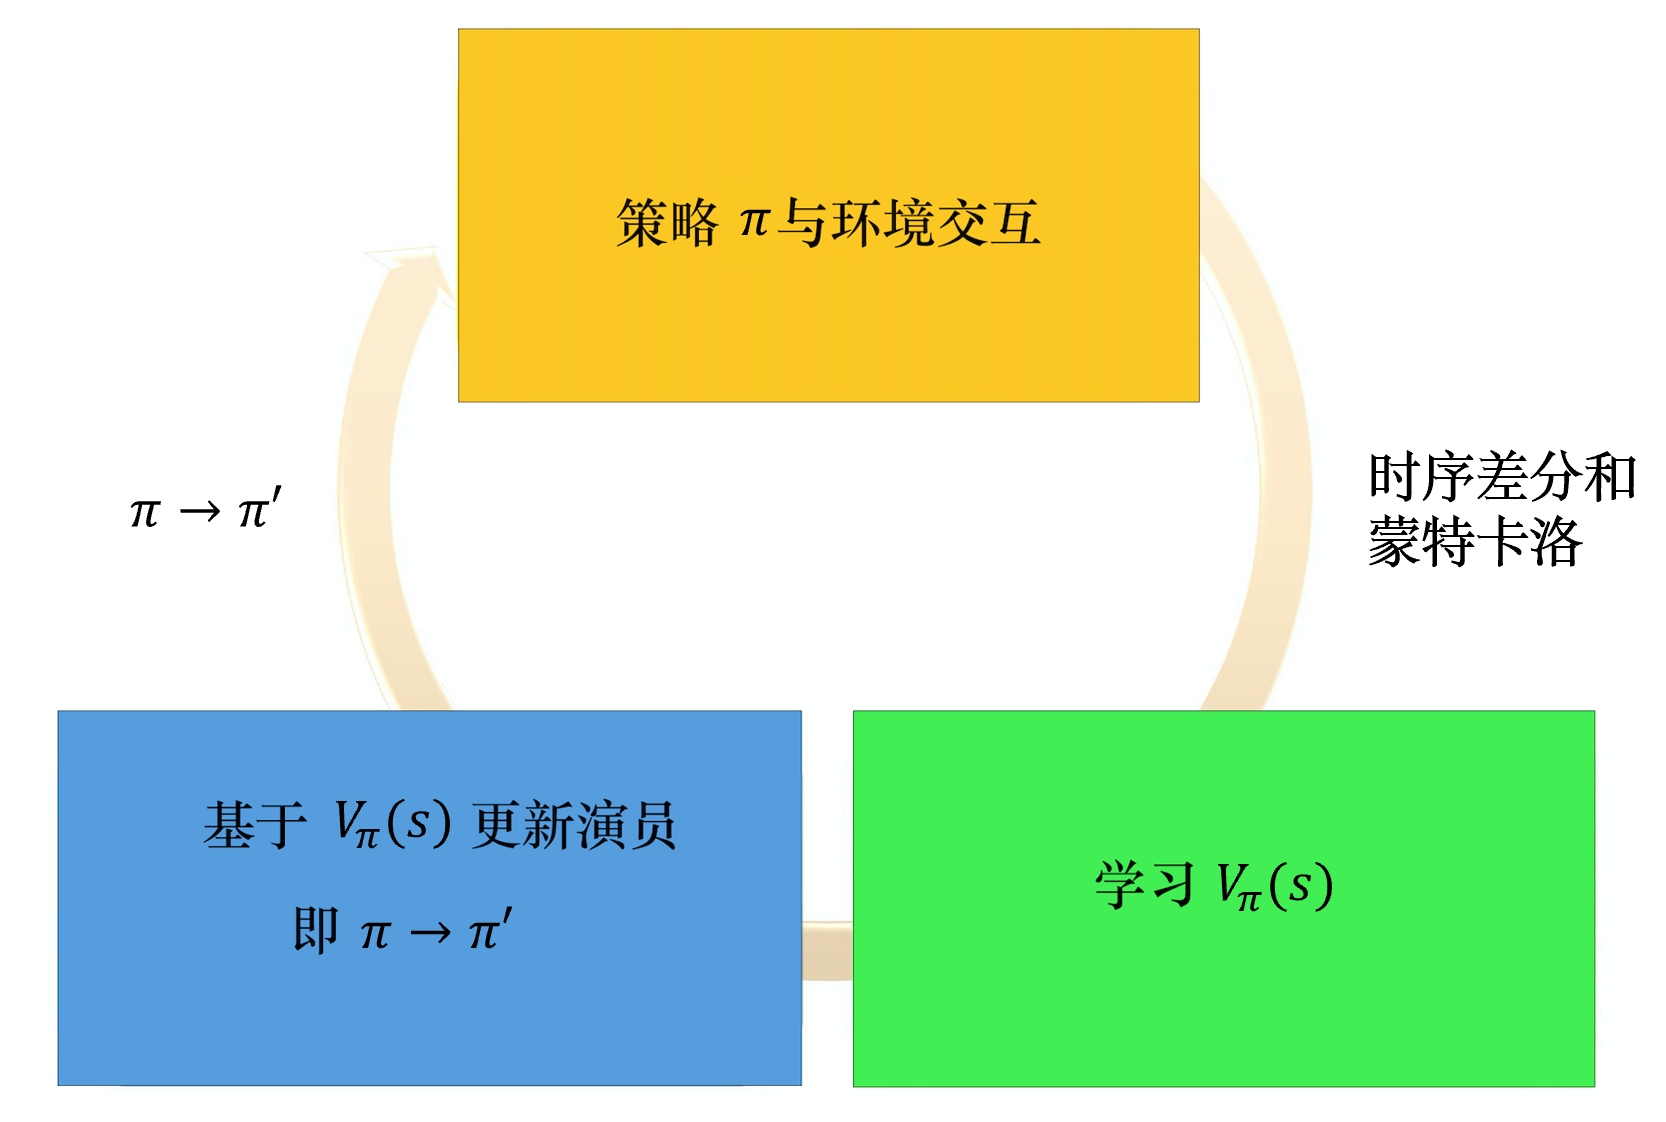
\includegraphics[width=0.4\linewidth]{res/ch9/9.5}
  \caption{优势评论员-评论员算法流程}
  \label{fig:fig9.5}
\end{figure}

实现优势演员-评论员算法的时候,有两个一定会用到的技巧。
第一个技巧是,我们需要估计两个网络:$V$ 网络和策略的网络(也就是演员)。
  评论员网络 $V_\pi(s)$ 接收一个状态,输出一个标量。
  演员的策略 $\pi(s)$ 接收一个状态,
  如果动作是离散的,输出就是一个动作的分布,
  如果动作是连续的,输出就是一个连续的向量。

\figref{fig:fig9.6} 所示为离散动作的例子,连续动作的情况也是一样的。输入一个状态,网络决定现在要采取哪一个动作。演员网络和评论员网络的输入都是 $s$,所以它们前面几个层(layer)是可以共享的。
\begin{figure}[h]
  \centering
  \includegraphics[width=0.5\linewidth]{res/ch9/9.6}
  \caption{离散动作的例子}
  \label{fig:fig9.6}
\end{figure}

尤其当我们在玩雅达利游戏时,输入都是图像。输入的图像非常复杂,通常我们在前期都会用一些卷积神经网络来处理它们,把图像抽象成高级(high level)的信息。把像素级别的信息抽象成高级信息的特征提取器,对于演员与评论员来说是可以共用的。所以通常我们会让演员与评论员共享前面几层,并且共用同一组参数,这一组参数大部分都是卷积神经网络的参数。
先把输入的像素变成比较高级的信息,再让演员决定要采取什么样的动作,让评论员即价值函数计算期望奖励。

第二个技巧是我们需要探索的机制。在演员-评论员算法中,有一个常见的探索的方法是对 $\pi$ 输出的分布设置一个约束。这个约束用于使分布的熵(entropy)不要太小,也就是希望不同的动作被采用的概率平均一些。这样在测试的时候,智能体才会多尝试各种不同的动作,才会把环境探索得比较好,从而得到比较好的结果。

\subsection{异步优势演员-评论员算法} 
强化学习有一个问题,就是它很慢,怎么提高训练的速度呢?例如,如\figref{fig:fig9.7} 所示,在动漫《火影忍者》中,有一次鸣人想要在一周之内打败晓,所以要加快修行的速度,鸣人的老师就教他一个方法:用影分身进行同样的修行。两个一起修行,经验值累积的速度就会变成两倍,所以鸣人就使用了 1000 个影分身来进行修行。这就是异步优势演员-评论员算法的体现。
\begin{figure}[hbt]
    \centering
    \includegraphics[width=0.5\linewidth]{res/ch9/9.7}
    \caption{影分身例子}
    \label{fig:fig9.7}
\end{figure}

异步优势演员-评论员算法同时使用很多个进程(worker),每一个进程就像一个影分身,最后这些影分身会把所有的经验值集合在一起。如果我们没有很多 CPU,不好实现异步优势演员-评论员算法,但可以实现优势演员-评论员算法。

异步优势演员-评论员算法的运作流程,如\figref{fig:fig9.8} 所示,
  异步优势演员-评论员算法一开始有一个全局网络(global network)。全局网络包含策略网络和价值网络,这两个网络是绑定(tie)在一起的,它们的前几个层会被绑在一起。
  假设全局网络的参数是 $\theta_1$,我们使用多个进程,每个进程用一张 CPU 去跑。比如我们有 8 个进程,则至少 8 张 CPU。每一个进程在工作前都会把全局网络的参数复制过来。
  接下来演员就与环境交互,每一个演员与环境交互的时候,都要收集到比较多样的数据。例如,如果是走迷宫,可能每一个演员起始的位置都会不一样,这样它们才能够收集到比较多样的数据。
  每一个演员与环境交互完之后,我们就会计算出梯度。计算出梯度以后,要用梯度去更新参数。我们就计算一下梯度,用梯度去更新全局网络的参数。就是这个进程算出梯度以后,就把梯度传回给中央的控制中心,中央的控制中心就会用这个梯度去更新原来的参数。
  
  注意,A3C使用了平行探索的方法,

  所有的演员都是平行跑的,每一个演员各做各的,不管彼此。所以每个演员都是去要了一个参数以后,做完就把参数传回去。当第一个进程做完想要把参数传回去的时候,本来它要的参数是 $\theta_1$,等它要把梯度传回去的时候,可能别人已经把原来的参数覆盖掉,变成 $\theta_2$了。但是没有关系,它一样会把这个梯度就覆盖过去。


\begin{figure}[hbt]
  \centering
  \includegraphics[width=0.4\linewidth]{res/ch9/9.8}
  \caption{异步优势演员-评论员算法的运作流程}
  \label{fig:fig9.8}
\end{figure}

\subsection{路径衍生策略梯度} 

接下来我们来了解\kw{路径衍生策略梯度(pathwise derivative policy gradient)}方法。这个方法可以看成 深度Q网络 解连续动作的一种特别的方法,也可以看成一种特别的演员-评论员的方法。
用动漫《棋魂》来比喻,阿光就是一个演员,佐为就是一个评论员。阿光落某一子以后,如果佐为是一般的演员-评论员算法的评论员,他会告诉阿光这时候不应该下小马步飞。佐为会告诉我们,我们现在采取的这一步算出来的值到底是好还是不好,但这样就结束了,他只告诉我们好还是不好。因为一般的演员-评论员算法的评论员就是输入状态或输入状态-动作对,给演员一个值,所以对演员来说,它只知道它做的这个动作到底是好还是不好。

但在路径衍生策略梯度里面,评论员会直接告诉演员采取什么样的动作才是好的。所以佐为不只是告诉阿光,这个时候不要下小马步飞,同时还告诉阿光这个时候应该要下大马步飞,这就是路径衍生策略梯度中的评论员所做的。评论员会直接告诉演员做什么样的动作才可以得到比较大的值。

% \begin{figure}[hbt]
%   \centering
%   \includegraphics[width=0.7\linewidth]{res/ch9/9.9}
%   \caption{路径衍生策略梯度}
%   \label{fig:fig9.9}
% \end{figure}

从 深度Q网络 的观点来看,深度Q网络 的一个问题是在使用 深度Q网络 时,考虑连续向量会比较麻烦,没有通用的解决方法(general solution),那我们应该怎么解这个优化问题呢?
我们用一个演员来解决这个优化的问题。本来在深度Q网络 里面,如果是一个连续的动作,我们要解决这个优化问题。但是现在这个优化问题由演员来解决,假设演员就是一个解决者(solver),这个解决者的工作就是对于给定的状态 $s$,解出来哪一个动作可以得到最大的 Q 值,这是从另外一个观点来看路径衍生策略梯度。
在 生成对抗网络 中也有类似的说法。我们学习一个判别器(discriminator)并用于评估时,是非常困难的,因为我们要解决的 arg max 的问题非常的困难,所以用生成器(generator)来生成。
所以概念是一样的,Q 就是那个判别器。根据这个判别器决定动作非常困难,怎么办?另外学习一个网络来解决这个优化问题,这个网络就是演员。
所以两个不同的观点是同一件事。从两个不同的观点来看,
一个观点是:我们可以对原来的深度Q网络 加以改进,学习一个演员来决定动作以解决 arg max 不好解的问题。
另外一个观点是:原来的演员-评论员算法的问题是评论员并没有给演员足够的信息,评论员只告诉演员好或不好的,没有告诉演员什么样是好,现在有新的方法可以直接告诉演员什么样的是好的。
路径衍生策略梯度算法如\figref{fig:fig9.10} 所示,假设我们学习了一个Q函数,Q函数的输入是 $s$ 与 $a$,输出是 $Q_{\pi}(s,a)$。接下来,我们要学习一个演员,这个演员的工作就是解决 arg max 的问题,即输入一个状态 $s$,希望可以输出一个动作 $a$。$a$ 被代入Q函数以后,它可以让 $Q_{\pi}(s,a)$ 尽可能大,即
\begin{equation}
  \label{eq:}
  \pi^{\prime}(s)=\underset{a}{\arg \max} Q_{\pi}(s, a)
\end{equation}

实际上在训练的时候,我们就是把 Q 与演员连接起来变成一个比较大的网络。Q 是一个网络,接收输入 $s$ 与 $a$,输出一个值。演员在训练的时候,它要做的事就是接收输入 $s$,输出 $a$。把 $a$ 代入 Q 中,希望输出的值越大越好。我们会固定住 Q 的参数,只调整演员的参数,用梯度上升的方法最大化 Q 的输出,这就是一个 生成对抗网络,即有条件的生成对抗网络(conditional GAN)。Q 就是判别器,但在强化学习里就是评论员,演员在 生成对抗网络 里面就是生成器。

\begin{figure}[hbt]
  \centering
  \includegraphics[width=0.5\linewidth]{res/ch9/9.10}
  \caption{路径衍生策略梯度}
  \label{fig:fig9.10}
\end{figure}


我们来看一下路径衍生策略梯度算法。如\figref{fig:fig9.11} 所示,一开始会有一个策略 $\pi$,它与环境交互并估计 Q 值。估计完 Q 值以后,我们就把 Q 值固定,只去学习一个演员。假设这个 Q 值估得很准,它知道在某一个状态采取什么样的动作会得到很大的Q值。接下来就学习这个演员,演员在给定 $s$ 的时候,采取了 $a$,可以让最后Q函数算出来的值越大越好。我们用准则(criteria)去更新策略 $\pi$,用新的 $\pi$ 与环境交互,再估计 Q值,得到新的 $\pi$ 去最大化 Q值的输出。深度Q网络 里面的技巧,在这里也几乎都用得上,比如经验回放、探索等技巧。

\begin{figure}[htb]
  \centering
  \includegraphics[width=0.5\linewidth]{res/ch9/9.11}
  \caption{路径衍生策略梯度算法}
  \label{fig:fig9.11}
\end{figure}

\figref{fig:fig9.12} 所示为原来深度Q网络 的算法。我们有一个Q函数 $Q$ 和另外一个目标Q函数 $\hat{Q}$。每一次训练,在每一个回合的每一个时间点,我们会看到一个状态 $s_t$,会采取某一个动作 $a_{t}$。至于采取哪一个动作是由Q函数所决定的。
如果是离散动作,我们看哪一个动作 $a$ 可以让 Q 值最大,就采取哪一个动作。当然,我们需要加一些探索,这样表现才会好。
我们会得到奖励 $r_t$,进入新的状态 $s_{t+1}$,然后把 $(s_t$,$a_{t}$,$r_t$,$s_{t+1})$ 放到回放缓冲区里。接下来,我们会从回放缓冲区中采样一个批量的数据,在这个批量数据里面,可能某一笔数据是 $(s_i, a_i, r_i, s_{i+1})$。接下来我们会算一个目标 $y$ ,$y=r_{i}+\max _{a} \hat{Q}\left(s_{i+1}, a\right)$。怎么学习 Q 呢?我们希望 $Q(s_i,a_i)$ 与 $y$ 越接近越好,这是一个回归问题,最后每 $C$ 步,要用 $Q$ 替代 $\hat{Q}$ 。

\begin{figure}[htb]
  \centering
  \includegraphics[width=0.5\linewidth]{res/ch9/9.12}
  \caption{深度Q网络算法}
  \label{fig:fig9.12}
\end{figure}

 接下来我们把深度Q网络 改成路径衍生策略梯度,需要做4个改变,如\figref{fig:fig9.13}所示。

(1)第一个改变是,我们要把 $Q$ 换成 $\theta$,本来是用 $Q$ 来决定在状态 $s_t$ 执行一个动作 $a_{t}$, 现在直接用 $\theta$ 来执行动作。
我们直接学习了一个演员。这个演员的输入 $s_t$ 会告诉我们应该采取哪一个 $a_{t}$。所以本来输入 $s_t$,采取哪一个 $a_t$是 Q 决定的,而在路径衍生策略梯度里面,我们会直接用 $\theta$ 来决定。

(2)第二个改变是,本来我们要计算在 $s_{i+1}$,根据策略采取某一个动作 $a$ 会得到的 Q 值,我们会采取让 $\hat{Q}$ 最大的那个动作 $a$。现在因为我们直接把 $s_{i+1}$ 代入$\theta$ ,就会知道给定 $s_{i+1}$ ,哪个动作会给我们最大的 Q值,就采取哪个动作。
在Q函数里面,有两个Q网络:真正的 Q网络和目标 Q 网络。实际上我们在实现路径衍生策略梯度算法的时候,也有两个演员:真正要学习的演员$\theta$和目标演员$\hat{\theta}$。这个原理就与为什么要有目标 Q 网络一样,我们在算目标值的时候,并不希望它一直的变动,所以我们会有一个目标演员和一个目标Q函数,它们平常的参数就是固定住的,这样可以让目标的值不会一直地变化。
% 所以本来到底是要用哪一个动作 $a$,我们会看说哪一个动作 $a$ 可以让 $\hat{Q}$  最大。但现在因为哪一个动作 $a$ 可以让 $\hat{Q}$ 最大这件事情已经用策略取代掉了,所以我们要知道哪一个动作 $a$ 可以让 $\hat{Q}$ 最大,就直接把那个状态代入 $\hat{\pi}$ 里面,看它得到哪一个 $a$,那个 $a$ 就是会让 $\hat{Q}(s,a)$ 的值最大的那个 $a$ 。
% 其实与原来的 深度Q网络 也是没什么不同,
总结一下,第二个改变是我们用策略取代原来要解 arg max 的地方。

(3)第三个改变是,之前只要学习 Q函数,现在我们多学习了一个 $\theta$,学习 $\theta$ 的目的是最大化Q函数,希望得到的演员可以让Q函数的输出尽可能大,这与学习 生成对抗网络 里面的生成器的概念是类似的。

(4)第四个改变是,我们不仅要取代目标的 Q 网络,还要取代目标策略。

\begin{figure}[hbt]
  \centering
  \includegraphics[width=0.5\linewidth]{res/ch9/9.13}
  \caption{从深度Q网络到路径衍生策略梯度}
  \label{fig:fig9.13}
\end{figure}

\subsection{与生成对抗网络的联系} 

如\tabref{tab:GAN_AC} 所示,GAN 与演员-评论员的方法是非常类似的。如果大家感兴趣,可以参考一篇论文:“Connecting Generative Adversarial Network and Actor-Critic Methods”。

生成对抗网络 与演员-评论员都挺难训练,所以在文献上就有各式各样的方法,告诉我们怎么样可以训练 生成对抗网络。
知道 生成对抗网络 与演员-评论员非常相似后,我们就可以知道怎样训练演员-评论员。但是因为做 生成对抗网络 与演员-评论员的人是两群人,所以这篇论文里面就列出说在 生成对抗网络 上面有哪些技术是有人做过的,在演员-评论员上面,有哪些技术是有人做过的。也许训练 生成对抗网络 的技术,我们可以试着应用在演员-评论员上,在演员-评论员上用过的技术,也可以试着应用在 生成对抗网络 上。

\begin{table}[hbt]
  \caption{与生成对抗网络的联系}
  \label{tab:GAN_AC}
  \centering
  \begin{tabular}{ccc}
  \toprule
  方法    & 生成对抗网络 & 演员-评论员 \\ \hline
  冻结学习  & 有      &  有    \\ 
  标签平滑  & 有     & 无      \\
  历史平均  &  有    & 无     \\ 
  小批量判别 &  有    & 无      \\ 
  批量归一化 &  有   &  有    \\ 
  目标网络  & 不适用    & 有      \\ 
  经验回放  & 无      & 有     \\ 
  熵正则化  & 无      & 有    \\ 
  兼容性   & 无      &  有   \\ 
  \bottomrule
  \end{tabular}
  \end{table}

% \begin{figure}[hbt]
%   \centering
%   \includegraphics[width=0.7\linewidth]{res/ch9/9.14}
%   \caption{与生成对抗网络的联系}
%   \label{fig:fig9.14}
% \end{figure}

\subsection{关键词}

优势演员-评论员(advantage actor-critic,A2C)算法:一种改进的演员-评论员(actor-critic)算法。

异步优势演员-评论员(asynchronous advantage actor-critic,A3C)算法:一种改进的演员-评论员算法,通过异步的操作,实现强化学习模型训练的加速。

路径衍生策略梯度(pathwise derivative policy gradient):一种使用Q学习来求解连续动作的算法,也是一种演员-评论员算法。其会对演员提供价值最大的动作,而不仅仅是提供某一个动作的好坏程度。


\subsection{习题}

\kw{9-1} 完整的优势演员-评论员算法的工作流程是怎样的?

\kw{9-2} 在实现演员-评论员算法的时候有哪些技巧?

\kw{9-3} 异步优势演员-评论员算法在训练时有很多的进程进行异步的工作,最后再将他们所获得的“结果”集合到一起。那么其具体是如何运作的呢?

\kw{9-4} 对比经典的Q学习算法,路径衍生策略梯度有哪些改进之处?

 
\subsection{面试题}

\kw{9-1} 友善的面试官:请简述一下异步优势演员-评论员算法(A3C),另外A3C是同策略还是异策略的模型呀?

\kw{9-2} 友善的面试官:请问演员-评论员算法有何优点呢?

\kw{9-3} 友善的面试官:请问异步优势演员-评论员算法具体是如何异步更新的?

\kw{9-4} 友善的面试官:演员-评论员算法中,演员和评论员两者的区别是什么?

\kw{9-5} 友善的面试官:演员-评论员算法框架中的评论员起了什么作用?

\kw{9-6} 友善的面试官:简述异步优势演员-评论员算法的优势函数。
  


% \subsection*{参考文献} 
% \begin{itemize}
%     \item \href{https://nndl.github.io/}{神经网络与深度学习}
% \end{itemize}



    % \section{稀疏奖励}
实际上用强化学习训练智能体的时候,多数时候智能体都不能得到奖励。在不能得到奖励的情况下,训练智能体是非常困难的。例如,假设我们要训练一个机器臂,桌上有一个螺丝钉与一个螺丝起子,要训练它用螺丝起子把螺丝钉栓进去很难,因为一开始智能体是什么都不知道,它唯一能够做不同的动作的原因是探索。例如,我们在做 Q学习 的时候会有一些随机性,让它去采取一些过去没有采取过的动作,要随机到,它把螺丝起子捡起来,再把螺丝栓进去,就会得到奖励1,这件事情是永远不可能发生的。所以,不管演员做了什么事情,它得到的奖励永远都是 0,对它来说不管采取什么样的动作都是一样糟或者是一样好。所以,它最后什么都不会学到。

如果环境中的奖励非常稀疏,强化学习的问题就会变得非常困难,但是人类可以在非常稀疏的奖励上去学习。人生通常多数的时候,就只是活在那里,都没有得到什么奖励或是惩罚。但是,人还是可以采取各种各样的行为。所以,一个真正厉害的人工智能应该能够在稀疏奖励的情况下也学到怎么与环境交互。

我们可以通过3个方向来解决稀疏奖励的问题,下面一一介绍。

\subsection{设计奖励}

第一个方向是\kw{设计奖励(reward shaping)}。环境有一个固定的奖励,它是真正的奖励,但是为了让智能体学到的结果是我们想要的,所以我们刻意设计了一些奖励来引导智能体。

例如,如\figref{fig:fig10.1} 所示,如果我们把小孩当成一个智能体,他可以采取两个动作:玩耍或者学习。
如果他玩耍,在下一个时间点就会得到奖励 1。但是他在月考的时候,成绩可能会很差,所以在 100 个小时之后,他会得到奖励 $-$100。
他也可以决定要学习,在下一个时间点,因为他没有玩耍,所以觉得很不爽,所以得到奖励 $-$1。但是在 100 个小时后,他可以得到奖励 100。对于一个小孩来说,他可能就会想要采取玩耍的动作而不是学习的动作。我们计算的是累积奖励,但也许对小孩来说,折扣因子会很大,所以他就不太在意未来的奖励。而且因为他是一个小孩,还没有很多经验,所以他的Q函数估计是非常不精准的。所以要他去估计很远以后会得到的累积奖励,他是估计不出来的。
这时候大人就要引导他,对他说:“如果你学习,我就给你一根棒棒糖。”对小孩来说,下一个时间点他得到的奖励就变成正的,他也许就会认为学习是比玩耍好的。虽然这并不是真正的奖励,而是其他人引导他的奖励。设计奖励的概念是一样的,简单来说,就是我们自己想办法设计一些奖励,这些奖励不是环境真正的奖励。在玩雅达利游戏时,真正的奖励是游戏主机给的奖励,但我们自己可以设计一些奖励引导智能体,让智能体做我们想要它做的事情。

\begin{figure}[htb]
    \centering
    \includegraphics[width=0.5\linewidth]{res/ch10/10.1}
    \caption{设计奖励}
    \label{fig:fig10.1}
\end{figure}

举个 Meta(原Facebook)玩 \textit{ViZDoom} 的智能体的例子。\textit{ViZDoom} 是一个第一人称射击游戏,在这个射击游戏中,杀了敌人得到正奖励,被杀得到负奖励。研究人员设计了一些新的奖励,用新的奖励来引导智能体让它们做得更好,这不是游戏中真正的奖励。比如掉血就扣分,弹药减少就扣分,捡到补给包就加分,待在原地就扣分,移动就加分。活着会扣一个很小的分数,因为如果不这样做,智能体会只想活着,一直躲避敌人,这样会让智能体好战一些。

设计奖励是有问题的,因为我们需要领域知识(domain knowledge)。例如,如\figref{fig:fig10.2} 所示,
机器人想要学会把蓝色的板子从柱子穿过。机器人很难学会,我们可以设计奖励。一个貌似合理的说法是,蓝色的板子离柱子越近,奖励越大。但是机器人靠近的方式会有问题,它会用蓝色的板子打柱子。而机器人要把蓝色板子放在柱子上面,才能让蓝色板子穿过柱子。因此,这种设计奖励的方式是有问题的。至于哪种设计奖励的方式有问题,哪种设计奖励的方式没问题,会变成一个领域知识,是我们要去调整的。

\begin{figure}[htb]
    \centering
    \includegraphics[width=0.5\linewidth]{res/ch10/10.2}
    \caption{设计奖励的问题}
    \label{fig:fig10.2}
\end{figure}

\subsection{好奇心}  

接下来介绍各种我们可以自己加入并且一般看起来是有用的奖励。例如,一种技术是给智能体加上好奇心(curiosity),称为\kw{好奇心驱动的奖励(curiosity driven reward)}。如\figref{fig:fig10.3} 所示,我们输入某个状态和某个动作到奖励函数中,奖励函数就会输出在这个状态采取这个动作会得到的奖励,总奖励越大越好。

在好奇心驱动的技术里面,我们会加上一个新的奖励函数------\kw{内在好奇心模块(intrinsic curiosity module,ICM)},它用于给智能体加上好奇心。内在好奇心模块需要 3 个输入:状态$s_1$、动作 $a_1$ 和状态$s_2$。根据输入,它会输出另外一个奖励$r_1^i$。对智能体来说,总奖励并不是只有 $r$,还有 $r^i$。它不是只把所有的 $r$ 都加起来,它还把所有 $r^i$ 加起来当作总奖励。所以在与环境交互的时候,它不是只希望 $r$ 越大越好,它还同时希望 $r^i$ 越大越好,它希望从内在好奇心模块里面得到的奖励越大越好。内在好奇心模块代表一种好奇心。

\begin{figure}[htb]
    \centering
    \includegraphics[width=0.5\linewidth]{res/ch10/10.3}
    \caption{好奇心}
    \label{fig:fig10.3}
\end{figure}

怎么设计内在好奇心模块?最原始的设计如\figref{fig:fig10.4} 所示,
内在好奇心模块的输入是现在的状态$s_t$、在这个状态采取的动作$a_t$以及下一个状态$s_{t+1}$,输出一个奖励$r^i_t$。那么 $r^i_t$  是怎么算出来的呢?在内在好奇心模块里面,我们有一个网络,这个网络会接收输入$a_t$ 与$s_t$,输出 $\hat{s}_{t+1}$,也就是这个网络根据 $a_t$ 和 $s_t$ 去预测  $\hat{s}_{t+1}$ 。然后再看这个网络的预测  $\hat{s}_{t+1}$ 与真实的情况 $s_{t+1}$ 的相似度,越不相似得到的奖励就越大。
所以奖励$r_t^i$ 的意思是,未来的状态越难被预测,得到的奖励就越大。这就是鼓励智能体去冒险、去探索,现在采取这个动作,未来会发生什么越难被预测,这个动作的奖励就越大。
所以如果有这样的内在好奇心模块,智能体就会倾向于采取一些风险比较大的动作,它想要去探索未知的世界。假设某一个状态是它没有办法预测的,它就会特别想要接近该状态,这可以提高智能体探索的能力。

网络 1 是另外训练出来的。训练的时候,我们会给网络 1 输入$a_t$、 $s_t$、 $s_{t+1}$,让网络 1 学习根据给定 $a_t$、$s_t$ 预测 $\hat{s}_{t+1}$。在智能体与环境交互的时候,我们要把内在好奇心模块固定住。这个想法有一个问题:某些状态很难被预测并不代表它就是好的、它就是应该要被尝试的。例如,俄罗斯轮盘的结果也是没有办法预测的,这并不代表人应该每天去玩俄罗斯轮盘。所以只鼓励智能体去冒险是不够的,因为如果仅仅只有这个网络的架构,智能体只知道什么东西它无法预测。如果在某一个状态采取某一个动作,智能体无法预测接下来结果,它就会采取那个动作,但这并不代表这样的结果一定是好的。例如,可能在某个游戏里面,背景会有风吹草动、会有树叶飘动这种无关紧要的事情。也许树叶飘动这件事,是很难被预测的,对智能体来说,它在某一个状态什么都不做,就看着树叶飘动,
发现树叶飘动是没有办法预测的,
接下来它就会一直看树叶飘动。所以智能体仅仅有好奇心是不够的,还要让它知道,什么事情是真正重要的。

\begin{figure}[htb]
    \centering
    \includegraphics[width=0.5\linewidth]{res/ch10/10.4}
    \caption{内在好奇心模块设计}
    \label{fig:fig10.4}
\end{figure}


怎么让智能体知道什么事情是真正重要的呢?我们要加上另外一个模块,我们要学习一个\kw{特征提取器(feature extractor)}。如\figref{fig:fig10.5} 所示,黄色的格子代表特征提取器,它输入一个状态,输出一个特征向量来代表这个状态,我们期待特征提取器可以把没有意义的画面,状态里面没有意义的东西过滤掉,比如风吹草动、白云的飘动以及树叶飘动。

假设特征提取器可以把无关紧要的信息过滤掉,网络 1 实际上做的事情是,给它一个演员和一个状态$s_t$ 的特征表示(feature representation),让它预测状态$s_{t+1}$ 的特征表示。接下来我们再来评价,这个预测的结果与真正的状态$s_{t+1}$ 的特征表示像不像,越不像,奖励就越大。怎么学习特征提取器呢?怎么让特征提取器把无关紧要的信息过滤掉呢?
我们可以学习另外一个网络,即网络 2。网络 2 把向量 $\pmb{\phi}(s_t)$和$\pmb{\phi}(s_{t+1})$ 作为输入,它要预测动作$a$ 是什么,它希望这个动作$a$ 与真正的动作$a$ 越接近越好。网络 2 会输出一个动作$a_t$,它会输出,从状态$s_t$ 到状态$s_{t+1}$,要采取的动作与真正的动作越接近越好。加上网络 2 是因为要用 $\pmb{\phi}(s_t)$、$\pmb{\phi}(s_{t+1})$  预测动作。所以,我们提取出来的特征与预测动作这件事情是有关的,风吹草动等与智能体要采取的动作无关的就会被过滤掉,就不会在被提取出来的向量中被表示。

\begin{figure}[htb]
    \centering
    \includegraphics[width=0.5\linewidth]{res/ch10/10.5}
    \caption{好奇心模块}
    \label{fig:fig10.5}
\end{figure}

\subsection{课程学习} 

第二个方向是\kw{课程学习(curriculum learning)} 。课程学习不是强化学习独有的概念,在机器学习尤其是深度学习中,我们都会用到课程学习的概念。具体来说,课程学习是指我们为智能体的学习做规划,给他“喂”的训练数据是有顺序的,通常都是由简单到难的。比如,假设我们要教一个小朋友学微积分,他做错题就惩罚他,这样他很难学会。我们应该先教他乘法,再教他微积分。所以课程学习就是指在训练智能体的时候,训练数据从简单到困难。就算不是强化学习,一般在训练深度网络的时候,我们有时候也会这么做。例如,在训练循环神经网络 的时候,已经有很多的文献都证明,给智能体先看短的序列,再慢慢给它看长的序列,通常它可以学得比较好。在强化学习里面,我们就是要帮智能体规划它的课程,课程难度从易到难。

例如,Meta玩 \textit{ViZDoom} 的智能体表现非常好,它参加 \textit{ViZDoom} 的比赛得了第一名。
对于 Meta 玩 \textit{ViZDoom} 的智能体,
是有为智能体规划课程的,从课程 0 一直到课程 7。在不同的课程里面,怪物的速度与血量是不一样的。所以,在越进阶的课程里面,怪物的速度越快,血量越多。如果直接上课程 7,智能体是无法学习的。要从课程 0 开始,一点一点增加难度,这样智能体才学得起来。

再例如,对于把蓝色的板子穿过柱子的任务,怎么让机器人一直从简单学到难呢?
如\figref{fig:fig10.6} (左)所示,也许一开始,板子就已经在柱子上了。这时候,机器人只要把蓝色的板子压下去就可以了。这种情况比较简单,机器人应该很快就能学会。因为机器人只有往上与往下这两个选择,往下就得到奖励,任务就结束了,所有它也不知道学的是什么。
如\figref{fig:fig10.6} (中)所示,我们把板子放高一点儿,机器人有时候会笨拙地往上拉板子,然后把板子拿出来。如果机器人可以学会压板子,拿板子也有很大的可能可以学会。假设机器人现在已经学到,只要板子接近柱子,它就可以把板子压下去。接下来,我们再让它学更一般的情况。
如\figref{fig:fig10.6} (右)所示,一开始,让板子离柱子远一点儿。然后,板子放到柱子上面的时候,机器人就知道把板子压下去,这就是课程学习的概念。当然课程学习有点儿特别,它需要人去为智能体设计课程。

\begin{figure}[htb]
    \centering
    \includegraphics[width=0.5\linewidth]{res/ch10/10.6}
    \caption{课程学习}
    \label{fig:fig10.6}
\end{figure}

有一个比较通用的方法:\kw{逆向课程生成(reverse curriculum generation)}。我们可以用一个比较通用的方法来帮智能体设计课程。
如\figref{fig:fig10.7} 所示,
假设我们一开始有一个状态$s_\mathrm{g}$,这是\kw{黄金状态(gold state)},也就是最后最理想的结果。如果以板子和柱子的实验为例,黄金状态就是把板子穿过柱子。如果我们以训练机械臂抓东西为例,抓到东西就称为黄金状态。接下来我们根据黄金状态去找其他的状态,这些其他的状态与黄金状态是比较接近的。例如,在让机械臂抓东西的例子里面,机械臂可能还没有抓到东西。假设与黄金状态很接近的状态称为 $s_1$。机械臂还没有抓到东西,但它与黄金状态很接近,这种状态可称为$s_1$。至于什么是接近,这取决于具体情况。我们要根据任务来设计怎么从 $s_\mathrm{g}$ 采样出 $s_1$。接下来,智能体再从 $s_1$ 开始与环境交互,看它能不能够达到黄金状态$s_\mathrm{g}$,在每一个状态下,智能体与环境交互的时候,都会得到一个奖励。

\begin{figure}[htb]
    \centering
    \includegraphics[width=0.5\linewidth]{res/ch10/10.7}
    \caption{逆向课程生成}
    \label{fig:fig10.7}
\end{figure}

接下来,我们把奖励特别极端的情况去掉。奖励特别极端的情况的意思是这些情况太简单或是太难了。如果奖励很大,就代表这个情况太简单了,就不用学习了,因为智能体已经会了,它可以得到很大的奖励。如果奖励太小,就代表这个情况太难了,依照智能体现在的能力它学不会,所以就不学这个,只学一些奖励适中的情况。

% 什么叫做适中,这个就是我们要调的参数,找一些奖励适中的情况。
接下来,再根据这些奖励适中的情况采样出更多的状态。假设一开始,机械臂在某个位置可以抓得到后。接下来,机械臂就再离远一点儿,看看能不能抓到;又能抓到后,再离远一点儿,看看能不能抓到。这是一个有用的方法,称为\kw{逆课程学习(reverse curriculum learning)}。前面讲的是课程学习,就是我们要为智能体规划学习的顺序。而逆课程学习是从黄金状态反推,如\figref{fig:fig10.8} 所示,就是从目标反推,所以这称为逆课程学习。  

\begin{figure}[htb]
    \centering
    \includegraphics[width=0.5\linewidth]{res/ch10/10.8}
    \caption{逆课程学习}
    \label{fig:fig10.8}
\end{figure}

\subsection{分层强化学习} 
第三个方向是\kw{分层强化学习(hierarchical reinforcement learning,HRL)}。分层强化学习是指,我们有多个智能体,一些智能体负责比较高级的东西,它们负责定目标,定完目标以后,再将目标分配给其他的智能体,让其他智能体来执行目标。
这样的想法也是很合理的。
例如,假设我们想写一篇论文,首先我们要想创新点,想完创新点后,还要做实验。做实验以后,我们要写论文。写完论文以后还要投稿、发表。每一个动作下面又会再细分,比如怎么做实验呢?我们要先收集数据,收集完数据以后,要标注标签,还要设计一个网络,
然后又训练不起来,要训练很多次。重新设计网络架构好几次,最后才把网络训练起来。
所以,我们要完成一个很大的任务的时候,并不是从非常底层的动作开始做,其实是有一个计划的。我们会先想,如果要完成这个最大的任务,要将之拆解成哪些小任务,每一个小任务要怎么拆解成更小的任务。例如,我们直接写一本书可能很困难,但先把一本书拆成几章,每章拆成几节,每节又拆成几段,每段又拆成几个句,这样可能就比较好写,这就是分层强化学习。

如\figref{fig:10.9a} 所示,例如,假设校长、教授和研究生都是智能体,并且我们所在的学校只要进入百大学校(QS排名前100的学校)就可以得到奖励。假设进入百大学校,校长就要提出愿景并告诉其他的智能体,现在我们要达到什么样的目标。校长的愿景可能是教授每年都要发3篇期刊。这些智能体都是分层的,所以上面的智能体,他的动作就是提出愿景。他把他的愿景传给下一层的智能体,下一层的智能体会接收这个愿景。
如果他下面还有其他智能体,他就会提出新的愿景。比如,校长要教授发期刊论文,但教授自己没时间实验,他也只能够让下面的研究生做实验。所以教授就提出愿景,做出实验的规划,研究生才是执行这个实验的人。把实验做出来以后,大家就可以得到奖励。现在是这样的,在学习的时候,每一个智能体都会学习,他们的整体目标就是要得到最后的奖励。前面的智能体,他们提出来的动作就是愿景。但是,假设他们提出来的愿景是下面的智能体达不到的,就会被讨厌。例如,教授都一直让研究生做一些很困难的实验,研究生做不出来,教授就会得到一个惩罚。所以如果下层的智能体没有办法达到上层智能体所提出来的目标,上层的智能体就会被讨厌,它就会得到一个负奖励。所以他要避免提出的那些愿景是下层的智能体做不到的。每一个智能体都把上层的智能体所提出的愿景当作输入,决定他自己要产生什么输出。

但是就算看到上面的愿景让我们做某件事情,最后也不一定能做成这件事情。如\figref{fig:10.9b} 所示,假设本来教授的目标是要发期刊论文,但他突然切换目标,要变成一个 YouTuber。这时,我们需要把原来的愿景改成变成 YouTuber。因为虽然本来的愿景是发期刊论文,但是后来变成 YouTuber,这些动作是没有被浪费的。我们就假设,本来的愿景就是要成为 YouTuber,我们就知道成为 YouTuber 要怎做了。这就是分层强化学习,是可以实现的技巧。

\begin{figure}[htb]
    \centering
    \includegraphics[width=0.5\linewidth]{res/ch10/10.9a}
    \caption{分层强化学习例子}
    \label{fig:10.9a}
\end{figure}

\begin{figure}[htb]
    \centering
    \includegraphics[width=0.5\linewidth]{res/ch10/10.9b}
    \caption{改变愿景}
    \label{fig:10.9b}
\end{figure}

\figref{fig:fig10.10} 是真实游戏的例子。第一个游戏是走迷宫,蓝色的是智能体,蓝色的智能体要走到黄色的目标。第二个游戏是单摆,单摆要碰到黄色的球。愿景是什么呢?
在走迷宫游戏里面,只有两个智能体,下层的智能体负责决定要怎么走,上层的智能体负责提出愿景。虽然,实际上我们可以用很多层,但这只用了两层。
走迷宫的游戏中粉红色的点代表的就是愿景。上层的智能体告诉蓝色的智能体,我们现在的第一个目标是先走到某个位置。蓝色的智能体到达以后,再说新的目标是走到另一个位置。蓝色的智能体再到达以后,新的目标会在其他位置。接下来蓝色的智能体又到达这个位置,最后希望蓝色的智能体可以到达黄色的位置。
单摆的例子也一样,粉红色的点代表的是上层的智能体所提出的愿景,所以这个智能体先摆到这边,接下来,新的愿景又跑到某个位置,所以它又摆到对应的位置。然后,新的愿景又跑到上面。然后又摆到上面,最后就走到黄色的位置。这就是分层强化学习。

\begin{figure}[htb]
    \centering
    \includegraphics[width=0.5\linewidth]{res/ch10/10.10}
    \caption{走迷宫和单摆的例子}
    \label{fig:fig10.10}
\end{figure}

最后,我们对分层强化学习进行总结。分层强化学习是指将一个复杂的强化学习问题分解成多个小的、简单的子问题,每个子问题都可以单独用马尔可夫决策过程来建模。这样,我们可以将智能体的策略分为高层次策略和低层次策略,高层次策略根据当前状态决定如何执行低层次策略。这样,智能体就可以解决一些非常复杂的任务。

\subsection{关键词}

设计奖励(reward shaping):当智能体与环境进行交互时,我们人为设计一些奖励,从而“指挥”智能体,告诉其采取哪一个动作是最优的。需要注意的是,这个奖励区别于环境的奖励。其可以提高我们估算Q函数时的准确性。

内在好奇心模块(intrinsic curiosity module,ICM):其代表好奇心驱动这个技术中的增加新的奖励函数以后的奖励函数。

课程学习(curriculum learning):一种广义的用在强化学习中训练智能体的方法,其在输入训练数据的时候,采取由易到难的顺序进行输入,也可以人为设计它的学习过程。这个方法在机器学习和强化学习中普遍使用。

逆课程学习(reverse curriculum learning):相较于课程学习,逆课程学习为更广义的方法。其从最终最理想的状态[我们称之为黄金状态(gold state)]开始,依次去寻找距离黄金状态最近的状态作为想让智能体达到的阶段性的“理想”状态。当然,我们会在此过程中有意地去掉一些极端的状态,即太简单、太难的状态。综上,逆课程学习是从黄金状态反推的方法。

分层强化学习(hierarchical reinforcement learning):将一个大型的任务,横向或者纵向地拆解成由多个智能体去执行的子任务。其中,有一些智能体负责比较高层次的任务,如负责定目标,定完目标后,再将目标分配给其他的智能体执行。


\subsection{习题}

\kw{10-1} 解决稀疏奖励的方法有哪些?

\kw{10-2} 设计奖励存在什么主要问题?

\kw{10-3} 内在好奇心模块是什么?我们应该如何设计内在好奇心模块?



\bibliographystyle{gbt7714-numerical}
\bibliography{ref.bib}

% \subsection*{参考文献} 
% \begin{itemize}
%     \item \href{https://nndl.github.io/}{神经网络与深度学习}
% \end{itemize}






    % 
\section{强化学习进阶}
\subsection{探索策略}
\subsection{逆强化学习}
\subsubsection{模仿学习}
\subsubsection{行为克隆}
\subsubsection{最大熵逆强化学习}
\subsection{分层强化学习}
\subsubsection{稀疏奖励}
\subsubsection{好奇心模块}
\subsubsection{课程学习}
\subsection{离线强化学习}
\subsection{多智能体强化学习}
\subsubsection{ QMIX 算法}
\subsubsection{ MADDPG 算法}
\subsubsection{ MAPPO 算法}

\subsection{关键词}
\subsection{习题}
\subsection{面试题}
\subsection{本章小结}
    % \section{深度确定性策略梯度} 

\subsection{离散动作与连续动作的区别} 

离散动作与连续动作是相对的概念,一个是可数的,一个是不可数的。 
如\figref{fig:fig12.1} 所示,离散动作和连续动作有几个例子。
在 \textit{CartPole} 环境中,可以有向左推小车、向右推小车两个动作。
在 \textit{Frozen Lake} 环境中,小乌龟可以有上、下、左、右4个动作。
在雅达利的 \textit{Pong} 游戏中,游戏有 6 个按键的动作可以输出。 
但在实际情况中,我们经常会遇到连续动作空间的情况,也就是输出的动作是不可数的。比如:推小车推力的大小、选择下一时刻方向盘转动的具体角度、给四轴飞行器的4个螺旋桨给的电压的大小。

\begin{figure}[hbt]
  \centering
  \includegraphics[width=0.7\linewidth]{res/ch12/12.1}
  \caption{离散动作和连续动作的区别}
  \label{fig:fig12.1}
\end{figure}

对于这些连续的动作,Q学习、深度Q网络等算法是没有办法处理的。那我们怎么输出连续的动作呢?这个时候,“万能”的神经网络又出现了。
如\figref{fig:fig12.2} 所示,在离散动作的场景下,比如我们输出上、下或是停止这几个动作。有几个动作,神经网络就输出几个概率值,我们用 $\pi_\theta(a_t|s_t)$ 来表示这个随机性的策略。
在连续的动作场景下,比如我们要输出机械臂弯曲的角度,我们就输出一个具体的浮点数。我们用 $\mu_{\theta}(s_t)$ 来代表这个确定性的策略。

我们再对随机性策略与确定性策略进行解释。
对随机性策略来说,输入某一个状态 $s$,采取某一个动作的可能性并不是百分之百的,而是有一个概率的(就好像抽奖一样),根据概率随机抽取一个动作。
而对于确定性策略来说,它不受概率的影响。当神经网络的参数固定之后,输入同样的状态,必然输出同样的动作,这就是确定性策略。
\begin{figure}[htb]
  \centering
  \includegraphics[width=0.7\linewidth]{res/ch12/12.2}
  \caption{使用神经网络处理连续动作与离散动作}
  \label{fig:fig12.2}
\end{figure}

如\figref{fig:fig12.3} 所示,
要输出离散动作,我们就加一个 softmax 层来确保所有的输出是动作概率,并且所有的动作概率和为 1。
要输出连续动作,我们一般可以在输出层加一层 tanh 函数。
tanh 函数的作用就是把输出限制到 [$-$1,1] 。
我们得到输出后,就可以根据实际动作的范围将其缩放,再输出给环境。
比如神经网络输出一个浮点数 2.8,经过 tanh 函数之后,它就可以被限制在 [$-$1,1] 之间,输出 0.99。假设小车速度的范围是 [$-$2,2] ,我们就按比例从 [$-$1,1] 扩大到 [$-$2,2],0.99 乘 2,最终输出的就是 1.98,将其作为小车的速度或者推小车的推力输出给环境。

\begin{figure}[htb]
  \centering
  \includegraphics[width=0.7\linewidth]{res/ch12/12.3}
  \caption{使用神经网络输出离散动作与连续动作}
  \label{fig:fig12.3}
\end{figure}

\subsection{深度确定性策略梯度} 

在连续控制领域,比较经典的强化学习算法就是\kw{深度确定性策略梯度(deep deterministic policy gradient,DDPG)}。如\figref{fig:fig12.4} 所示,DDPG 的特点可以从它的名字中拆解出来,拆解成深度、确定性和策略梯度。

深度是因为用了神经网络;
确定性表示 DDPG 输出的是一个确定性的动作,可以用于有连续动作的环境;
策略梯度代表的是它用到的是策略网络。REINFORCE 算法每隔一个回合就更新一次,但 DDPG 是每个步骤都会更新一次策略网络,它是一个单步更新的策略网络。

\begin{figure}[hbt]
  \centering
  \includegraphics[width=0.5\linewidth]{res/ch12/12.4}
  \caption{DDPG}
  \label{fig:fig12.4}
\end{figure}


DDPG 是 深度Q网络的一个扩展版本,可以扩展到连续动作空间。
在 DDPG 的训练中,它借鉴了 深度Q网络 的技巧:目标网络和经验回放。
经验回放与 深度Q网络 是一样的,但目标网络的更新与 深度Q网络 的有点儿不一样。
提出 DDPG 是为了让 深度Q网络 可以扩展到连续的动作空间,就是我们刚才提到的小车速度、角度和电压等这样的连续值。如\figref{fig:fig12.5} 所示,
DDPG 在 深度Q网络 基础上加了一个策略网络来直接输出动作值,所以 DDPG 需要一边学习 Q 网络,一边学习策略网络。
Q 网络的参数用 $w$ 来表示。策略网络的参数用 $\theta$ 来表示。
我们称这样的结构为演员-评论员的结构。

\begin{figure}[hbt]
  \centering
  \includegraphics[width=0.5\linewidth]{res/ch12/12.5}
  \caption{从深度Q网络到DDPG}
  \label{fig:fig12.5}
\end{figure}

通俗地解释一下演员-评论员结构。如\figref{fig:fig12.6} 所示,
策略网络扮演的就是演员的角色,它负责对外展示输出,输出动作。
Q 网络就是评论员,它会在每一个步骤都对演员输出的动作做一个评估,打一个分,估计演员的动作未来能有多少奖励,也就是估计演员输出的动作的 Q 值大概是多少,即 $Q_w(s,a)$。演员需要根据舞台目前的状态来做出一个动作。
评论员就是评委,它需要根据舞台现在的状态和演员输出的动作对演员刚刚的表现去打一个分数 $Q_w(s,a)$。
演员根据评委的打分来调整自己的策略,也就是更新演员的神经网络参数 $\theta$,争取下次可以做得更好。
评论员则要根据观众的反馈,也就是环境的反馈奖励来调整自己的打分策略,也就是要更新评论员的神经网络的参数 $w$ ,
评论员的最终目标是让演员的表演获得观众尽可能多的欢呼声和掌声,从而最大化未来的总收益。

最开始训练的时候,这两个神经网络的参数是随机的。所以评论员最开始是随机打分的,演员也随机输出动作。但是由于有环境反馈的奖励存在,因此评论员的评分会越来越准确,所评判的演员的表现也会越来越好。
既然演员是一个神经网络,是我们希望训练好的策略网络,我们就需要计算梯度来更新优化它里面的参数 $\theta$ 。简单来说,我们希望调整演员的网络参数,使得评委打分尽可能高。注意,这里的演员是不关注观众的,它只关注评委,它只迎合评委的打分 $Q_w(s,a)$。

\begin{figure}[hbt]
  \centering
  \includegraphics[width=0.5\linewidth]{res/ch12/12.6}
  \caption{演员-评论员结构通俗解释}
  \label{fig:fig12.6}
\end{figure}


深度Q网络与DDPG的联系如\figref{fig:fig12.7} 所示。
深度Q网络 的最佳策略是想要学出一个很好的 Q 网络,学出这个网络之后,我们希望选取的那个动作使 Q 值最大。
DDPG 的目的也是求解让 Q 值最大的那个动作。
演员只是为了迎合评委的打分而已,所以优化策略网络的梯度就是要最大化这个 Q 值,所以构造的损失函数就是让 Q 取一个负号。
我们写代码的时候把这个损失函数放入优化器里面,它就会自动最小化损失,也就是最大化 Q。

这里要注意,除了策略网络要做优化,DDPG 还有一个 Q 网络也要优化。
评论员一开始也不知道怎么评分,它也是在一步一步的学习当中,慢慢地给出准确的分数。
我们优化 Q 网络的方法其实与 深度Q网络 优化 Q 网络的方法是一样的,我们用真实的奖励$r$ 和下一步的 $Q$ 即 $Q^{\prime}$ 来拟合未来的奖励 $Q\_\text{target}$。
然后让 Q 网络的输出逼近 $Q\_\text{target}$。
所以构造的损失函数就是直接求这两个值的均方差。
构造好损失函数后,我们将其放到优化器中,让它自动最小化损失。


\begin{figure}[hbt]
  \centering
  \includegraphics[width=0.7\linewidth]{res/ch12/12.7}
  \caption{深度Q网络与DDPG的联系}
  \label{fig:fig12.7}
\end{figure}

如\figref{fig:fig12.8} 所示,我们可以把两个网络的损失函数构造出来。
策略网络的损失函数是一个复合函数。我们把 $a = \mu_\theta(s)$ 代入,最终策略网络要优化的是策略网络的参数 $\theta$ 。Q 网络要优化的是 $Q_w(s,a)$ 和 $Q\_\text{target}$ 之间的一个均方差。
但是 Q 网络的优化存在一个和 深度Q网络 一模一样的问题就是它后面的 $Q\_\text{target}$ 是不稳定的。此外,后面的 $Q_{\bar{w}}\left(s^{\prime}, a^{\prime}\right)$ 也是不稳定的,因为 $Q_{\bar{w}}\left(s^{\prime}, a^{\prime}\right)$ 也是一个预估的值。

为了使 $Q\_\text{target}$ 更加稳定,DDPG 分别给 Q 网络和策略网络搭建了目标网络,即target\_Q网络和target\_P策略网络。
$\text{target}\_Q$ 网络是为了计算 $Q\_\text{target}$ 中 $Q_{\bar{w}}\left(s^{\prime}, a^{\prime}\right)$。
$Q_{\bar{w}}\left(s^{\prime}, a^{\prime}\right)$ 里面的需要的下一个动作 $a'$  是通过 $\text{target}\_P$ 网络输出的,即 $a^{\prime}=\mu_{\bar{\theta}}\left(s^{\prime}\right)$。
Q 网络和策略网络的参数是$w$,$\text{target}\_Q$ 网络和 $\text{target}\_P$ 策略网络的参数是 $\bar{w}$。
DDPG 有4个网络,策略网络的目标网络 和 Q 网络的目标网络是颜色比较深的这两个,它们只是为了让计算 $Q\_\text{target}$ 更稳定。因为这两个网络也是固定一段时间的参数之后再与评估网络同步最新的参数。

这里训练需要用到的数据就是 $s$、$a$、$r$、$s'$,我们只需要用到这4个数据。我们用回放缓冲区把这些数据存起来,然后采样进行训练。经验回放的技巧与 深度Q网络 中的是一样的。注意,因为 DDPG 使用了经验回放技巧,所以 DDPG 是一个异策略的算法。

\begin{figure}[hbt]
  \centering
  \includegraphics[width=0.7\linewidth]{res/ch12/12.8}
  \caption{目标网络和经验回放}
  \label{fig:fig12.8}
\end{figure}

DDPG通过异策略的方式来训练一个确定性策略。因为策略是确定的,所以如果智能体使用同策略来探索,在一开始的时候,它很可能不会尝试足够多的动作来找到有用的学习信号。为了让 DDPG 的策略更好地探索,我们在训练的时候给它们的动作加了噪声。DDPG 的原作者推荐使用时间相关的 \href{https://en.wikipedia.org/wiki/Ornstein–Uhlenbeck_process}{OU 噪声},但最近的结果表明不相关的、均值为 0 的高斯噪声的效果非常好。由于后者更简单,因此我们更喜欢使用它。为了便于获得更高质量的训练数据,我们可以在训练过程中把噪声变小。
在测试的时候,为了查看策略利用它学到的东西的表现,我们不会在动作中加噪声。

\subsection{双延迟深度确定性策略梯度} 

虽然 DDPG 有时表现很好,但它对于超参数和其他类型的调整方面经常很敏感。
如\figref{fig:fig12.9} 所示,DDPG常见的问题是已经学习好的 Q 函数开始显著地高估 Q 值,然后导致策略被破坏,因为它利用了 Q 函数中的误差。

\begin{figure}[hbt]
  \centering
  \subfloat[Hopper-v1]{
    \label{fig:12.9a}
    \includegraphics[width=0.3\linewidth]{res/ch12/12.9a}
  }
  \subfloat[Walker2d-v1]{
    \label{fig:12.9b}
    \includegraphics[width=0.3\linewidth]{res/ch12/12.9b}
  }
  \caption{DDPG的问题\upcite{td3_paper}}

  \label{fig:fig12.9}
\end{figure}

我们可以使用实际的 Q 值与Q网络输出的 Q 值进行对比。实际的 Q 值可以用蒙特卡洛来算。根据当前的策略采样 1000 条轨迹,得到 $G$ 后取平均值,进而得到实际的 Q 值。

\kw{双延迟深度确定性策略梯度(twin delayed DDPG,TD3)}通过引入3个关键技巧来解决这个问题。
\begin{itemize}
\item \kw{截断的双 Q 学习(clipped dobule Q-learning)} 。TD3学习两个Q函数(因此名字中有 “twin”)。TD3通过最小化均方差来同时学习两个Q函数:$Q_{\phi_1}$ 和 $Q_{\phi_2}$。两个Q函数都使用一个目标,两个Q函数中给出的较小的值会被作为如下的 Q-target:

$$
y\left(r, s^{\prime}, d\right)=r+\gamma(1-d) \min _{i=1,2} Q_{\phi_{i, \text{targ}}}\left(s^{\prime}, a_\text{TD3}\left(s^{\prime}\right)\right)
$$

\item \kw{延迟的策略更新(delayed policy updates)} 。相关实验结果表明,同步训练动作网络和评价网络,却不使用目标网络,会导致训练过程不稳定;但是仅固定动作网络时,评价网络往往能够收敛到正确的结果。因此 TD3算法以较低的频率更新动作网络,以较高的频率更新评价网络,通常每更新两次评价网络就更新一次策略。
\item  \kw{目标策略平滑(target policy smoothing)}。TD3引入了平滑化(smoothing)思想。TD3在目标动作中加入噪声,通过平滑 Q 沿动作的变化,使策略更难利用 Q 函数的误差。
\end{itemize}

这3个技巧加在一起,使得性能相比基线 DDPG 有了大幅的提升。


目标策略平滑化的工作原理如下:
$$
a_\text{TD3}\left(s^{\prime}\right)=\operatorname{clip}\left(\mu_{\theta, \text{targ}}\left(s^{\prime}\right)+\operatorname{clip}(\epsilon,-c, c), a_{\text {low }}, a_{\text {high }}\right)
$$
其中 $\epsilon$ 本质上是一个噪声,是从正态分布中取样得到的,即 $\epsilon \sim N(0,\sigma)$。
目标策略平滑化是一种正则化方法。

如\figref{fig:fig12.10} 所示,我们可以将 TD3 算法与其他算法进行对比。TD3算法的作者自己实现的 深度确定性策略梯度(图中为our DDPG)和官方实现的 DDPG 的表现不一样,这说明 DDPG 对初始化和调参非常敏感。
TD3对参数不是这么敏感。在TD3的论文中,TD3的性能比\kw{软演员-评论员(soft actor-critic,SAC)}高。软演员-评论员又被译作软动作评价。
但在SAC的论文中, SAC 的性能比TD3 高,这是因为强化学习的很多算法估计对参数和初始条件敏感。

\begin{figure}[hbt]
  \centering
  \includegraphics[width=0.7\linewidth]{res/ch12/12.10}
  \caption{TD3与其他算法对比\upcite{td3_paper}}
  \label{fig:fig12.10}
\end{figure}

TD3的作者给出了其对应PyTorch的实现,见\url{https://github.com/sfujim/TD3/},代码写得很棒,我们可以将其作为一个强化学习的标准库来学习。
TD3以异策略的方式训练确定性策略。由于该策略是确定性的,因此如果智能体要探索策略,则一开始它可能不会尝试采取足够广泛的动作来找到有用的学习信号。为了使TD3策略更好地探索,我们在训练时在它们的动作中添加了噪声,通常是不相关的均值为0的高斯噪声。为了便于获取高质量的训练数据,我们可以在训练过程中减小噪声的大小。
在测试时,为了查看策略对所学知识的利用程度,我们不会在动作中增加噪声。


\subsection{使用深度确定性策略梯度解决倒立摆问题}

前面章节都是离散动作的环境,但实际中也有很多连续动作的环境,比如 OpenAI Gym 中的 Pendulum-v1 环境,它解决的是一个倒立摆问题,我们先对该环境做一个简要说明。

\subsubsection{ Pendulum-v1 简介}

如果说 CartPole-v0 是一个离散动作的经典入门环境,那么 Pendulum-v1 就是连续动作的经典入门环境。如\figref{fig:pendulum_1} 所示,我们通过施加力矩使摆阵向上摆动并保持直立。

\begin{figure}[htb]
    \centering
    \includegraphics[width=0.3\linewidth]{res/ch12/assets/pendulum_1.png}
    \caption{Pendulum-v1环境}
    \label{fig:pendulum_1}
\end{figure}
该环境的状态数有三个,设摆针在竖直方向上的顺时针旋转角为$\theta$,$\theta$设在$[\mathrm{\pi},\mathrm{\pi}]$之间,则相应的状态为$[cos\theta,sin\theta,\dot{\theta}]$,即表示角度和角速度.我们的动作则是一个 $-2$ 到 $2$ 之间的力矩,它是一个连续量,因而该环境不能用离散动作的算法比如深度 Q 网络算法来解决。奖励是根据相关的物理原理而计算出的等式,如下:

$$
-\left(\theta^{2}+0.1 \times \hat{\theta}^{2}+0.001 \times \text { action }^{2}\right)
$$

对于每一步,其最低奖励为$-\left(\mathrm{\pi}^{2}+0.1 \times 8^{2}+0.001 \times 2^{2}\right)= -16.2736044$,最高奖励为0。同 CartPole-v0 环境一样,达到最优算法的情况下,每回合的步数是无限的,因此这里设定每回合最大步数为200以便于训练。

\subsubsection{ 深度确定性策略梯度基本接口}

我们依然使用接口的概念,通过伪代码分析并实现 DDPG 的训练模式,如\figref{fig:ddpg} 所示。

\begin{figure}[htb]
    \centering
    \includegraphics[width=0.75\linewidth]{res/ch12/assets/ddpg.png}
    \caption{深度确定性策略梯度算法}
    \label{fig:ddpg}
\end{figure}

代码如下:

\begin{lstlisting}[style=Python]
    ou_noise = OUNoise(env.action_space)  # 动作噪声
    rewards = [] # 记录奖励
    ma_rewards = []  # 记录滑动平均奖励
    for i_ep in range(cfg.train_eps):
        state = env.reset()
        ou_noise.reset()
        done = False
        ep_reward = 0
        i_step = 0
        while not done:
            i_step += 1
            action = agent.choose_action(state)
            action = ou_noise.get_action(action, i_step) 
            next_state, reward, done, _ = env.step(action)
            ep_reward += reward
            agent.memory.push(state, action, reward, next_state, done)
            agent.update()
            state = next_state
        if (i_ep+1)%10 == 0:
            print('回合:{}/{},奖励:{}'.format(i_ep+1, cfg.train_eps, ep_reward))
        rewards.append(ep_reward)
        if ma_rewards:
            ma_rewards.append(0.9*ma_rewards[-1]+0.1*ep_reward)
        else:
            ma_rewards.append(ep_reward)
\end{lstlisting}

相比于 深度Q网络 , DDPG 主要更新了两部分,一是给动作施加噪声,另外是软更新策略,即最后一步。

\subsubsection{ Ornstein-Uhlenbeck 噪声}

奥恩斯坦-乌伦贝克(Ornstein-Uhlenbeck,OU)噪声适用于惯性系统,尤其是时间离散化粒度较小的情况。 OU 噪声是一种随机过程,下面略去证明,直接给出公式。对于当前时刻$t$的一个变量$x$,其下一时刻$x(t+\Delta t)$:
$$
x(t+\Delta t)=x(t)-\theta(x(t)-\mu) \Delta t+\sigma W_t
$$
其中 $W_t$ 属于正态分布,OU 噪声代码实现如下:

\begin{lstlisting}[style=Python]
    class OUNoise(object):
        '''Ornstein–Uhlenbeck噪声
        '''
        def __init__(self, action_space, mu=0.0, theta=0.15, max_sigma=0.3, min_sigma=0.3, decay_period=100000):
            self.mu           = mu # OU噪声的参数
            self.theta        = theta # OU噪声的参数
            self.sigma        = max_sigma # OU噪声的参数
            self.max_sigma    = max_sigma
            self.min_sigma    = min_sigma
            self.decay_period = decay_period
            self.action_dim   = action_space.shape[0]
            self.low          = action_space.low
            self.high         = action_space.high
            self.reset()
        def reset(self):
            self.obs = np.ones(self.action_dim) * self.mu
        def evolve_obs(self):
            x  = self.obs
            dx = self.theta * (self.mu - x) + self.sigma * np.random.randn(self.action_dim)
            self.obs = x + dx
            return self.obs
        def get_action(self, action, t=0):
            ou_obs = self.evolve_obs()
            self.sigma = self.max_sigma - (self.max_sigma - self.min_sigma) * min(1.0, t / self.decay_period) # sigma会逐渐衰减
            return np.clip(action + ou_obs, self.low, self.high) # 动作加上噪声后进行剪切
\end{lstlisting}

\subsubsection{深度确定性策略梯度算法}

 DDPG 算法主要也包括两个功能,一个是选择动作,另外一个是更新策略,首先看选择动作:

\begin{lstlisting}[style=Python]
    def choose_action(self, state):
        state = torch.FloatTensor(state).unsqueeze(0).to(self.device)
        action = self.actor(state)
        return action.detach().cpu().numpy()[0, 0]
\end{lstlisting}

由于 DDPG 是直接从演员网络取得动作,因此这里不用$\varepsilon$-贪心策略。在更新策略函数中,也会与 深度Q网络 稍有不同,并且加入软更新:

\begin{lstlisting}[style=Python]
    def update(self):
        if len(self.memory) < self.batch_size: # 当 memory 中不满足一个批量时,不更新策略
            return
        # 从回放缓冲区中随机采样一个批量的经验
        state, action, reward, next_state, done = self.memory.sample(self.batch_size)
        # 转变为张量
        state = torch.FloatTensor(state).to(self.device)
        next_state = torch.FloatTensor(next_state).to(self.device)
        action = torch.FloatTensor(action).to(self.device)
        reward = torch.FloatTensor(reward).unsqueeze(1).to(self.device)
        done = torch.FloatTensor(np.float32(done)).unsqueeze(1).to(self.device)
        # 计算期望Q值
        policy_loss = self.critic(state, self.actor(state))
        policy_loss = -policy_loss.mean()
        next_action = self.target_actor(next_state)
        target_value = self.target_critic(next_state, next_action.detach())
        expected_value = reward + (1.0 - done) * self.gamma * target_value
        expected_value = torch.clamp(expected_value, -np.inf, np.inf)
        value = self.critic(state, action)
        value_loss = nn.MSELoss()(value, expected_value.detach())
        self.actor_optimizer.zero_grad()
        policy_loss.backward()
        self.actor_optimizer.step()
        self.critic_optimizer.zero_grad()
        value_loss.backward()
        self.critic_optimizer.step()
        # 软更新
        for target_param, param in zip(self.target_critic.parameters(), self.critic.parameters()):
            target_param.data.copy_(target_param.data * (1.0 - self.soft_tau) +param.data * self.soft_tau)
        for target_param, param in zip(self.target_actor.parameters(), self.actor.parameters()):
            target_param.data.copy_(target_param.data * (1.0 - self.soft_tau) +param.data * self.soft_tau)
\end{lstlisting}

\subsubsection{结果分析}

实现算法之后,我们先看看训练效果,如\figref{fig:train_rewards_curve_cn-1760758} 所示。

\begin{figure}[htb]
    \centering
    \includegraphics[width=0.6\linewidth]{res/ch12/assets/train_rewards_curve_cn-1760758.png}
    \caption{Pendulum-v1 环境下DDPG算法的训练曲线}
    \label{fig:train_rewards_curve_cn-1760758}
\end{figure}


可以看到算法整体上是收敛的,但是稳定状态下波动还比较大,依然有提升的空间。限于笔者的精力,这里只是帮助读者实现一个基础的代码演示,想要使得算法调到最优,感兴趣的读者可以多思考实现。我们再来看看测试的结果,如\figref{fig:eval_rewards_curve_cn-1760950} 所示。

\begin{figure}[htb]
    \centering
    \includegraphics[width=0.6\linewidth]{res/ch12/assets/eval_rewards_curve_cn-1760950.png}
    \caption{Pendulum-v1 环境下DDPG算法的测试曲线}
    \label{fig:eval_rewards_curve_cn-1760950}
\end{figure}

从\figref{fig:eval_rewards_curve_cn-1760950} 中看出测试的滑动平均奖励在$-150$左右,但其实训练的时候平均的稳态奖励在$-300$左右,这是因为在测试的时候我们舍去了 OU 噪声。

\subsection{关键词}

深度确定性策略梯度(deep deterministic policy gradient,DDPG):在连续控制领域经典的强化学习算法,是深度Q网络在处理连续动作空间的一个扩充方法。具体地,从命名就可以看出,“深度”表明使用了深度神经网络;“确定性”表示其输出的是一个确定的动作,可以用于连续动作环境;“策略梯度”代表的是它用到的是策略网络,并且每步都会更新一次,其是一个单步更新的策略网络。其与深度Q网络都有目标网络和经验回放的技巧,在经验回放部分是一致的,在目标网络的更新上有些许不同。


\subsection{习题}

\kw{12-1} 请解释随机性策略和确定性策略,两者有什么区别?

\kw{12-2} 对于连续动作的控制空间和离散动作的控制空间,如果我们都采取策略网络,应该分别如何操作?


\subsection{面试题}

\kw{12-1} 友善的面试官:请简述一下深度确定性策略梯度算法。

\kw{12-2} 友善的面试官:请问深度确定性策略梯度算法是同策略算法还是异策略算法?请说明具体原因并分析。

\kw{12-3} 友善的面试官:你是否了解过分布的分布式深度确定性策略梯度算法(distributed distributional deep deterministic policy gradient,D4PG)呢?请描述一下吧。


\bibliographystyle{gbt7714-numerical}
\bibliography{ref.bib}


    % \appendix
\section{附录A习题解答}
\section{附录B面试题解答}

\end{document}
